\documentclass[twoside]{book}

% Packages required by doxygen
\usepackage{fixltx2e}
\usepackage{calc}
\usepackage{doxygen}
\usepackage[export]{adjustbox} % also loads graphicx
\usepackage{graphicx}
\usepackage[utf8]{inputenc}
\usepackage{makeidx}
\usepackage{multicol}
\usepackage{multirow}
\PassOptionsToPackage{warn}{textcomp}
\usepackage{textcomp}
\usepackage[nointegrals]{wasysym}
\usepackage[table]{xcolor}

% Font selection
\usepackage[T1]{fontenc}
\usepackage[scaled=.90]{helvet}
\usepackage{courier}
\usepackage{amssymb}
\usepackage{sectsty}
\renewcommand{\familydefault}{\sfdefault}
\allsectionsfont{%
  \fontseries{bc}\selectfont%
  \color{darkgray}%
}
\renewcommand{\DoxyLabelFont}{%
  \fontseries{bc}\selectfont%
  \color{darkgray}%
}
\newcommand{\+}{\discretionary{\mbox{\scriptsize$\hookleftarrow$}}{}{}}

% Page & text layout
\usepackage{geometry}
\geometry{%
  a4paper,%
  top=2.5cm,%
  bottom=2.5cm,%
  left=2.5cm,%
  right=2.5cm%
}
\tolerance=750
\hfuzz=15pt
\hbadness=750
\setlength{\emergencystretch}{15pt}
\setlength{\parindent}{0cm}
\setlength{\parskip}{3ex plus 2ex minus 2ex}
\makeatletter
\renewcommand{\paragraph}{%
  \@startsection{paragraph}{4}{0ex}{-1.0ex}{1.0ex}{%
    \normalfont\normalsize\bfseries\SS@parafont%
  }%
}
\renewcommand{\subparagraph}{%
  \@startsection{subparagraph}{5}{0ex}{-1.0ex}{1.0ex}{%
    \normalfont\normalsize\bfseries\SS@subparafont%
  }%
}
\makeatother

% Headers & footers
\usepackage{fancyhdr}
\pagestyle{fancyplain}
\fancyhead[LE]{\fancyplain{}{\bfseries\thepage}}
\fancyhead[CE]{\fancyplain{}{}}
\fancyhead[RE]{\fancyplain{}{\bfseries\leftmark}}
\fancyhead[LO]{\fancyplain{}{\bfseries\rightmark}}
\fancyhead[CO]{\fancyplain{}{}}
\fancyhead[RO]{\fancyplain{}{\bfseries\thepage}}
\fancyfoot[LE]{\fancyplain{}{}}
\fancyfoot[CE]{\fancyplain{}{}}
\fancyfoot[RE]{\fancyplain{}{\bfseries\scriptsize Generated by Doxygen }}
\fancyfoot[LO]{\fancyplain{}{\bfseries\scriptsize Generated by Doxygen }}
\fancyfoot[CO]{\fancyplain{}{}}
\fancyfoot[RO]{\fancyplain{}{}}
\renewcommand{\footrulewidth}{0.4pt}
\renewcommand{\chaptermark}[1]{%
  \markboth{#1}{}%
}
\renewcommand{\sectionmark}[1]{%
  \markright{\thesection\ #1}%
}

% Indices & bibliography
\usepackage{natbib}
\usepackage[titles]{tocloft}
\setcounter{tocdepth}{3}
\setcounter{secnumdepth}{5}
\makeindex

% Hyperlinks (required, but should be loaded last)
\usepackage{ifpdf}
\ifpdf
  \usepackage[pdftex,pagebackref=true]{hyperref}
\else
  \usepackage[ps2pdf,pagebackref=true]{hyperref}
\fi
\hypersetup{%
  colorlinks=true,%
  linkcolor=blue,%
  citecolor=blue,%
  unicode%
}

% Custom commands
\newcommand{\clearemptydoublepage}{%
  \newpage{\pagestyle{empty}\cleardoublepage}%
}

\usepackage{caption}
\captionsetup{labelsep=space,justification=centering,font={bf},singlelinecheck=off,skip=4pt,position=top}

%===== C O N T E N T S =====

\begin{document}

% Titlepage & ToC
\hypersetup{pageanchor=false,
             bookmarksnumbered=true,
             pdfencoding=unicode
            }
\pagenumbering{alph}
\begin{titlepage}
\vspace*{7cm}
\begin{center}%
{\Large Compresor i descompressor }\\
\vspace*{1cm}
{\large Generated by Doxygen 1.8.13}\\
\end{center}
\end{titlepage}
\clearemptydoublepage
\pagenumbering{roman}
\tableofcontents
\clearemptydoublepage
\pagenumbering{arabic}
\hypersetup{pageanchor=true}

%--- Begin generated contents ---
\chapter{Compresor i Descompresor}
\label{index}\hypertarget{index}{}\subsection*{Utilitzem els següents algoritmes\+:}


\begin{DoxyEnumerate}
\item L\+Z78
\item \href{./classdomini_1_1algorithm_1_1JPEG.html}{\tt J\+P\+EG }
\end{DoxyEnumerate}

\subsection*{aixo es la main page H\+EM DE F\+ER C\+O\+S\+ES}
\chapter{Hierarchical Index}
\section{Class Hierarchy}
This inheritance list is sorted roughly, but not completely, alphabetically\+:\begin{DoxyCompactList}
\item \contentsline{section}{domini.\+utils.\+Array\+Circular}{\pageref{classdomini_1_1utils_1_1ArrayCircular}}{}
\item \contentsline{section}{domini.\+utils.\+Bin\+Tree}{\pageref{classdomini_1_1utils_1_1BinTree}}{}
\item \contentsline{section}{domini.\+utils.\+byte\+To\+Conversion}{\pageref{classdomini_1_1utils_1_1byteToConversion}}{}
\item \contentsline{section}{domini.\+algorithm.\+Ctrl\+\_\+\+Algorithm}{\pageref{classdomini_1_1algorithm_1_1Ctrl__Algorithm}}{}
\item \contentsline{section}{persistencia.\+input.\+Ctrl\+\_\+\+Input}{\pageref{classpersistencia_1_1input_1_1Ctrl__Input}}{}
\begin{DoxyCompactList}
\item \contentsline{section}{persistencia.\+input.\+Ctrl\+\_\+\+Input\+\_\+\+Img}{\pageref{classpersistencia_1_1input_1_1Ctrl__Input__Img}}{}
\item \contentsline{section}{persistencia.\+input.\+Ctrl\+\_\+\+Input\+\_\+\+J\+P\+EG}{\pageref{classpersistencia_1_1input_1_1Ctrl__Input__JPEG}}{}
\item \contentsline{section}{persistencia.\+input.\+Ctrl\+\_\+\+Input\+\_\+\+L\+Z78}{\pageref{classpersistencia_1_1input_1_1Ctrl__Input__LZ78}}{}
\item \contentsline{section}{persistencia.\+input.\+Ctrl\+\_\+\+Input\+\_\+\+L\+Z\+SS}{\pageref{classpersistencia_1_1input_1_1Ctrl__Input__LZSS}}{}
\item \contentsline{section}{persistencia.\+input.\+Ctrl\+\_\+\+Input\+\_\+\+L\+ZW}{\pageref{classpersistencia_1_1input_1_1Ctrl__Input__LZW}}{}
\item \contentsline{section}{persistencia.\+input.\+Ctrl\+\_\+\+Input\+\_\+\+Text}{\pageref{classpersistencia_1_1input_1_1Ctrl__Input__Text}}{}
\end{DoxyCompactList}
\item \contentsline{section}{presentacion.\+master.\+Ctrl\+\_\+\+Master}{\pageref{classpresentacion_1_1master_1_1Ctrl__Master}}{}
\item \contentsline{section}{persistencia.\+output.\+Ctrl\+\_\+\+Output}{\pageref{classpersistencia_1_1output_1_1Ctrl__Output}}{}
\begin{DoxyCompactList}
\item \contentsline{section}{persistencia.\+output.\+Ctrl\+\_\+\+Output\+\_\+\+Img}{\pageref{classpersistencia_1_1output_1_1Ctrl__Output__Img}}{}
\end{DoxyCompactList}
\item \contentsline{section}{domini.\+utils.\+Dict\+\_\+\+Decode}{\pageref{classdomini_1_1utils_1_1Dict__Decode}}{}
\item \contentsline{section}{domini.\+utils.\+Dict\+\_\+\+Encode}{\pageref{classdomini_1_1utils_1_1Dict__Encode}}{}
\item \contentsline{section}{domini.\+utils.\+Driver\+\_\+\+\_\+\+Array\+Circular}{\pageref{classdomini_1_1utils_1_1Driver____ArrayCircular}}{}
\item \contentsline{section}{domini.\+utils.\+Driver\+\_\+\+\_\+\+Bin\+Tree}{\pageref{classdomini_1_1utils_1_1Driver____BinTree}}{}
\item \contentsline{section}{domini.\+utils.\+Driver\+\_\+\+\_\+byte\+To\+Conversion}{\pageref{classdomini_1_1utils_1_1Driver____byteToConversion}}{}
\item \contentsline{section}{domini.\+algorithm.\+Driver\+\_\+\+\_\+\+Ctrl\+\_\+\+Algorithm}{\pageref{classdomini_1_1algorithm_1_1Driver____Ctrl__Algorithm}}{}
\item \contentsline{section}{persistencia.\+input.\+Driver\+\_\+\+\_\+\+Ctrl\+\_\+\+Input\+\_\+\+L\+Z78}{\pageref{classpersistencia_1_1input_1_1Driver____Ctrl__Input__LZ78}}{}
\item \contentsline{section}{persistencia.\+input.\+Driver\+\_\+\+\_\+\+Ctrl\+\_\+\+Input\+\_\+\+L\+Z\+SS}{\pageref{classpersistencia_1_1input_1_1Driver____Ctrl__Input__LZSS}}{}
\item \contentsline{section}{persistencia.\+input.\+Driver\+\_\+\+\_\+\+Ctrl\+\_\+\+Input\+\_\+\+L\+ZW}{\pageref{classpersistencia_1_1input_1_1Driver____Ctrl__Input__LZW}}{}
\item \contentsline{section}{presentacion.\+master.\+Driver\+\_\+\+\_\+\+Ctrl\+\_\+\+Master}{\pageref{classpresentacion_1_1master_1_1Driver____Ctrl__Master}}{}
\item \contentsline{section}{persistencia.\+output.\+Driver\+\_\+\+\_\+\+Ctrl\+\_\+\+Output}{\pageref{classpersistencia_1_1output_1_1Driver____Ctrl__Output}}{}
\item \contentsline{section}{domini.\+utils.\+Driver\+\_\+\+\_\+\+Dict\+\_\+\+Decode}{\pageref{classdomini_1_1utils_1_1Driver____Dict__Decode}}{}
\item \contentsline{section}{domini.\+utils.\+Driver\+\_\+\+\_\+\+Dict\+\_\+\+Encode}{\pageref{classdomini_1_1utils_1_1Driver____Dict__Encode}}{}
\item \contentsline{section}{domini.\+estadistica.\+Driver\+\_\+\+\_\+\+Estadistica}{\pageref{classdomini_1_1estadistica_1_1Driver____Estadistica}}{}
\item \contentsline{section}{persistencia.\+input.\+Driver\+\_\+\+\_\+\+Input}{\pageref{classpersistencia_1_1input_1_1Driver____Input}}{}
\item \contentsline{section}{persistencia.\+input.\+Driver\+\_\+\+\_\+\+Input\+\_\+\+Text}{\pageref{classpersistencia_1_1input_1_1Driver____Input__Text}}{}
\item \contentsline{section}{domini.\+utils.\+Driver\+\_\+\+\_\+\+Intor\+Byte}{\pageref{classdomini_1_1utils_1_1Driver____IntorByte}}{}
\item \contentsline{section}{domini.\+algorithm.\+Driver\+\_\+\+\_\+\+L\+Z78}{\pageref{classdomini_1_1algorithm_1_1Driver____LZ78}}{}
\item \contentsline{section}{domini.\+algorithm.\+Driver\+\_\+\+\_\+\+L\+Z\+SS}{\pageref{classdomini_1_1algorithm_1_1Driver____LZSS}}{}
\item \contentsline{section}{domini.\+algorithm.\+Driver\+\_\+\+\_\+\+L\+ZW}{\pageref{classdomini_1_1algorithm_1_1Driver____LZW}}{}
\item \contentsline{section}{domini.\+utils.\+Driver\+\_\+\+\_\+\+Node}{\pageref{classdomini_1_1utils_1_1Driver____Node}}{}
\item \contentsline{section}{persistencia.\+output.\+Driver\+\_\+\+\_\+\+Output}{\pageref{classpersistencia_1_1output_1_1Driver____Output}}{}
\item \contentsline{section}{domini.\+utils.\+Driver\+\_\+\+\_\+\+Pair}{\pageref{classdomini_1_1utils_1_1Driver____Pair}}{}
\item \contentsline{section}{domini.\+utils.\+Driver\+\_\+\+\_\+\+Trie}{\pageref{classdomini_1_1utils_1_1Driver____Trie}}{}
\item \contentsline{section}{domini.\+utils.\+Driver\+\_\+\+\_\+\+Trie\+Node}{\pageref{classdomini_1_1utils_1_1Driver____TrieNode}}{}
\item \contentsline{section}{domini.\+estadistica.\+Estadistica}{\pageref{classdomini_1_1estadistica_1_1Estadistica}}{}
\item \contentsline{section}{domini.\+algorithm.\+Huffman}{\pageref{classdomini_1_1algorithm_1_1Huffman}}{}
\item \contentsline{section}{persistencia.\+input.\+Input}{\pageref{classpersistencia_1_1input_1_1Input}}{}
\item \contentsline{section}{persistencia.\+input.\+Input\+\_\+\+Text}{\pageref{classpersistencia_1_1input_1_1Input__Text}}{}
\item \contentsline{section}{domini.\+utils.\+Intor\+Byte}{\pageref{classdomini_1_1utils_1_1IntorByte}}{}
\item \contentsline{section}{domini.\+algorithm.\+J\+P\+EG}{\pageref{classdomini_1_1algorithm_1_1JPEG}}{}
\item \contentsline{section}{domini.\+algorithm.\+L\+Z78}{\pageref{classdomini_1_1algorithm_1_1LZ78}}{}
\item \contentsline{section}{domini.\+algorithm.\+L\+Z\+SS}{\pageref{classdomini_1_1algorithm_1_1LZSS}}{}
\item \contentsline{section}{domini.\+algorithm.\+L\+ZW}{\pageref{classdomini_1_1algorithm_1_1LZW}}{}
\item \contentsline{section}{domini.\+algorithm.\+L\+Z\+W\+Test}{\pageref{classdomini_1_1algorithm_1_1LZWTest}}{}
\item \contentsline{section}{Main}{\pageref{classMain}}{}
\item \contentsline{section}{domini.\+utils.\+Node}{\pageref{classdomini_1_1utils_1_1Node}}{}
\item \contentsline{section}{persistencia.\+output.\+Output}{\pageref{classpersistencia_1_1output_1_1Output}}{}
\item \contentsline{section}{domini.\+utils.\+Pair$<$ T1, T2 $>$}{\pageref{classdomini_1_1utils_1_1Pair}}{}
\item \contentsline{section}{domini.\+utils.\+string\+Conversion}{\pageref{classdomini_1_1utils_1_1stringConversion}}{}
\item \contentsline{section}{domini.\+utils.\+Trie$<$ T $>$}{\pageref{classdomini_1_1utils_1_1Trie}}{}
\item \contentsline{section}{domini.\+utils.\+Trie\+Node$<$ T $>$}{\pageref{classdomini_1_1utils_1_1TrieNode}}{}
\end{DoxyCompactList}

\chapter{Class Index}
\section{Class List}
Here are the classes, structs, unions and interfaces with brief descriptions\+:\begin{DoxyCompactList}
\item\contentsline{section}{\hyperlink{classdomini_1_1utils_1_1ArrayCircular}{domini.\+utils.\+Array\+Circular} \\*Aquesta és la classe per a estructura de dades del algoritme L\+Z\+SS }{\pageref{classdomini_1_1utils_1_1ArrayCircular}}{}
\item\contentsline{section}{\hyperlink{classdomini_1_1utils_1_1BinTree}{domini.\+utils.\+Bin\+Tree} }{\pageref{classdomini_1_1utils_1_1BinTree}}{}
\item\contentsline{section}{\hyperlink{classdomini_1_1utils_1_1byteToConversion}{domini.\+utils.\+byte\+To\+Conversion} \\*Classe \hyperlink{classdomini_1_1utils_1_1byteToConversion}{byte\+To\+Conversion} }{\pageref{classdomini_1_1utils_1_1byteToConversion}}{}
\item\contentsline{section}{\hyperlink{classdomini_1_1algorithm_1_1Ctrl__Algorithm}{domini.\+algorithm.\+Ctrl\+\_\+\+Algorithm} \\*Classe de \hyperlink{classdomini_1_1algorithm_1_1Ctrl__Algorithm}{Ctrl\+\_\+\+Algorithm} }{\pageref{classdomini_1_1algorithm_1_1Ctrl__Algorithm}}{}
\item\contentsline{section}{\hyperlink{classpersistencia_1_1input_1_1Ctrl__Input}{persistencia.\+input.\+Ctrl\+\_\+\+Input} \\*Classe de \hyperlink{classpersistencia_1_1input_1_1Ctrl__Input}{Ctrl\+\_\+\+Input} }{\pageref{classpersistencia_1_1input_1_1Ctrl__Input}}{}
\item\contentsline{section}{\hyperlink{classpersistencia_1_1input_1_1Ctrl__Input__Img}{persistencia.\+input.\+Ctrl\+\_\+\+Input\+\_\+\+Img} }{\pageref{classpersistencia_1_1input_1_1Ctrl__Input__Img}}{}
\item\contentsline{section}{\hyperlink{classpersistencia_1_1input_1_1Ctrl__Input__JPEG}{persistencia.\+input.\+Ctrl\+\_\+\+Input\+\_\+\+J\+P\+EG} }{\pageref{classpersistencia_1_1input_1_1Ctrl__Input__JPEG}}{}
\item\contentsline{section}{\hyperlink{classpersistencia_1_1input_1_1Ctrl__Input__LZ78}{persistencia.\+input.\+Ctrl\+\_\+\+Input\+\_\+\+L\+Z78} \\*Acces a un arxiu comprimit amb L\+Z78 }{\pageref{classpersistencia_1_1input_1_1Ctrl__Input__LZ78}}{}
\item\contentsline{section}{\hyperlink{classpersistencia_1_1input_1_1Ctrl__Input__LZSS}{persistencia.\+input.\+Ctrl\+\_\+\+Input\+\_\+\+L\+Z\+SS} \\*Aquesta és la classe fill del controlador \hyperlink{classpersistencia_1_1input_1_1Ctrl__Input}{Ctrl\+\_\+\+Input} }{\pageref{classpersistencia_1_1input_1_1Ctrl__Input__LZSS}}{}
\item\contentsline{section}{\hyperlink{classpersistencia_1_1input_1_1Ctrl__Input__LZW}{persistencia.\+input.\+Ctrl\+\_\+\+Input\+\_\+\+L\+ZW} \\*Acces a un arxiu comprimit amb L\+ZW }{\pageref{classpersistencia_1_1input_1_1Ctrl__Input__LZW}}{}
\item\contentsline{section}{\hyperlink{classpersistencia_1_1input_1_1Ctrl__Input__Text}{persistencia.\+input.\+Ctrl\+\_\+\+Input\+\_\+\+Text} \\*Classe de \hyperlink{classpersistencia_1_1input_1_1Ctrl__Input__Text}{Ctrl\+\_\+\+Input\+\_\+\+Text} }{\pageref{classpersistencia_1_1input_1_1Ctrl__Input__Text}}{}
\item\contentsline{section}{\hyperlink{classpresentacion_1_1master_1_1Ctrl__Master}{presentacion.\+master.\+Ctrl\+\_\+\+Master} \\*Classe \hyperlink{classpresentacion_1_1master_1_1Ctrl__Master}{Ctrl\+\_\+\+Master} }{\pageref{classpresentacion_1_1master_1_1Ctrl__Master}}{}
\item\contentsline{section}{\hyperlink{classpersistencia_1_1output_1_1Ctrl__Output}{persistencia.\+output.\+Ctrl\+\_\+\+Output} \\*Classe \hyperlink{classpersistencia_1_1output_1_1Ctrl__Output}{Ctrl\+\_\+\+Output} }{\pageref{classpersistencia_1_1output_1_1Ctrl__Output}}{}
\item\contentsline{section}{\hyperlink{classpersistencia_1_1output_1_1Ctrl__Output__Img}{persistencia.\+output.\+Ctrl\+\_\+\+Output\+\_\+\+Img} }{\pageref{classpersistencia_1_1output_1_1Ctrl__Output__Img}}{}
\item\contentsline{section}{\hyperlink{classdomini_1_1utils_1_1Dict__Decode}{domini.\+utils.\+Dict\+\_\+\+Decode} \\*Diccionari (amb els mètodes corresponents) emprat per a la descompressió amb L\+ZW }{\pageref{classdomini_1_1utils_1_1Dict__Decode}}{}
\item\contentsline{section}{\hyperlink{classdomini_1_1utils_1_1Dict__Encode}{domini.\+utils.\+Dict\+\_\+\+Encode} \\*Diccionari (amb els mètodes corresponents) emprat per a la compressió amb L\+ZW }{\pageref{classdomini_1_1utils_1_1Dict__Encode}}{}
\item\contentsline{section}{\hyperlink{classdomini_1_1utils_1_1Driver____ArrayCircular}{domini.\+utils.\+Driver\+\_\+\+\_\+\+Array\+Circular} \\*Driver de \hyperlink{classdomini_1_1utils_1_1ArrayCircular}{Array\+Circular} }{\pageref{classdomini_1_1utils_1_1Driver____ArrayCircular}}{}
\item\contentsline{section}{\hyperlink{classdomini_1_1utils_1_1Driver____BinTree}{domini.\+utils.\+Driver\+\_\+\+\_\+\+Bin\+Tree} }{\pageref{classdomini_1_1utils_1_1Driver____BinTree}}{}
\item\contentsline{section}{\hyperlink{classdomini_1_1utils_1_1Driver____byteToConversion}{domini.\+utils.\+Driver\+\_\+\+\_\+byte\+To\+Conversion} \\*Driver de \hyperlink{classdomini_1_1utils_1_1byteToConversion}{byte\+To\+Conversion} }{\pageref{classdomini_1_1utils_1_1Driver____byteToConversion}}{}
\item\contentsline{section}{\hyperlink{classdomini_1_1algorithm_1_1Driver____Ctrl__Algorithm}{domini.\+algorithm.\+Driver\+\_\+\+\_\+\+Ctrl\+\_\+\+Algorithm} \\*Driver de \hyperlink{classdomini_1_1algorithm_1_1Ctrl__Algorithm}{Ctrl\+\_\+\+Algorithm} }{\pageref{classdomini_1_1algorithm_1_1Driver____Ctrl__Algorithm}}{}
\item\contentsline{section}{\hyperlink{classpersistencia_1_1input_1_1Driver____Ctrl__Input__Img}{persistencia.\+input.\+Driver\+\_\+\+\_\+\+Ctrl\+\_\+\+Input\+\_\+\+Img} \\*Driver de \hyperlink{classpersistencia_1_1input_1_1Ctrl__Input__Img}{Ctrl\+\_\+\+Input\+\_\+\+Img} }{\pageref{classpersistencia_1_1input_1_1Driver____Ctrl__Input__Img}}{}
\item\contentsline{section}{\hyperlink{classpersistencia_1_1input_1_1Driver____Ctrl__Input__JPEG}{persistencia.\+input.\+Driver\+\_\+\+\_\+\+Ctrl\+\_\+\+Input\+\_\+\+J\+P\+EG} \\*Driver de \hyperlink{classpersistencia_1_1input_1_1Ctrl__Input__JPEG}{Ctrl\+\_\+\+Input\+\_\+\+J\+P\+EG} }{\pageref{classpersistencia_1_1input_1_1Driver____Ctrl__Input__JPEG}}{}
\item\contentsline{section}{\hyperlink{classpersistencia_1_1input_1_1Driver____Ctrl__Input__LZ78}{persistencia.\+input.\+Driver\+\_\+\+\_\+\+Ctrl\+\_\+\+Input\+\_\+\+L\+Z78} \\*Driver de \hyperlink{classpersistencia_1_1input_1_1Ctrl__Input__LZ78}{Ctrl\+\_\+\+Input\+\_\+\+L\+Z78} }{\pageref{classpersistencia_1_1input_1_1Driver____Ctrl__Input__LZ78}}{}
\item\contentsline{section}{\hyperlink{classpersistencia_1_1input_1_1Driver____Ctrl__Input__LZSS}{persistencia.\+input.\+Driver\+\_\+\+\_\+\+Ctrl\+\_\+\+Input\+\_\+\+L\+Z\+SS} \\*Driver de \hyperlink{classpersistencia_1_1input_1_1Ctrl__Input__LZSS}{Ctrl\+\_\+\+Input\+\_\+\+L\+Z\+SS} }{\pageref{classpersistencia_1_1input_1_1Driver____Ctrl__Input__LZSS}}{}
\item\contentsline{section}{\hyperlink{classpersistencia_1_1input_1_1Driver____Ctrl__Input__LZW}{persistencia.\+input.\+Driver\+\_\+\+\_\+\+Ctrl\+\_\+\+Input\+\_\+\+L\+ZW} \\*Driver de \hyperlink{classpersistencia_1_1input_1_1Ctrl__Input__LZW}{Ctrl\+\_\+\+Input\+\_\+\+L\+ZW} }{\pageref{classpersistencia_1_1input_1_1Driver____Ctrl__Input__LZW}}{}
\item\contentsline{section}{\hyperlink{classpresentacion_1_1master_1_1Driver____Ctrl__Master}{presentacion.\+master.\+Driver\+\_\+\+\_\+\+Ctrl\+\_\+\+Master} \\*Driver de \hyperlink{classpresentacion_1_1master_1_1Ctrl__Master}{Ctrl\+\_\+\+Master} }{\pageref{classpresentacion_1_1master_1_1Driver____Ctrl__Master}}{}
\item\contentsline{section}{\hyperlink{classpersistencia_1_1output_1_1Driver____Ctrl__Output}{persistencia.\+output.\+Driver\+\_\+\+\_\+\+Ctrl\+\_\+\+Output} \\*Driver per la classe \hyperlink{classpersistencia_1_1output_1_1Ctrl__Output}{Ctrl\+\_\+\+Output} }{\pageref{classpersistencia_1_1output_1_1Driver____Ctrl__Output}}{}
\item\contentsline{section}{\hyperlink{classpersistencia_1_1output_1_1Driver____Ctrl__Output__Img}{persistencia.\+output.\+Driver\+\_\+\+\_\+\+Ctrl\+\_\+\+Output\+\_\+\+Img} \\*Driver de \hyperlink{classpersistencia_1_1output_1_1Ctrl__Output__Img}{Ctrl\+\_\+\+Output\+\_\+\+Img} }{\pageref{classpersistencia_1_1output_1_1Driver____Ctrl__Output__Img}}{}
\item\contentsline{section}{\hyperlink{classdomini_1_1utils_1_1Driver____Dict__Decode}{domini.\+utils.\+Driver\+\_\+\+\_\+\+Dict\+\_\+\+Decode} \\*Driver de \hyperlink{classdomini_1_1utils_1_1Dict__Decode}{Dict\+\_\+\+Decode} }{\pageref{classdomini_1_1utils_1_1Driver____Dict__Decode}}{}
\item\contentsline{section}{\hyperlink{classdomini_1_1utils_1_1Driver____Dict__Encode}{domini.\+utils.\+Driver\+\_\+\+\_\+\+Dict\+\_\+\+Encode} \\*Driver de \hyperlink{classdomini_1_1utils_1_1Dict__Encode}{Dict\+\_\+\+Encode} }{\pageref{classdomini_1_1utils_1_1Driver____Dict__Encode}}{}
\item\contentsline{section}{\hyperlink{classdomini_1_1estadistica_1_1Driver____Estadistica}{domini.\+estadistica.\+Driver\+\_\+\+\_\+\+Estadistica} \\*Driver de \hyperlink{classdomini_1_1estadistica_1_1Estadistica}{Estadistica} }{\pageref{classdomini_1_1estadistica_1_1Driver____Estadistica}}{}
\item\contentsline{section}{\hyperlink{classdomini_1_1algorithm_1_1Driver____Huffman}{domini.\+algorithm.\+Driver\+\_\+\+\_\+\+Huffman} \\*Driver de \hyperlink{classdomini_1_1algorithm_1_1Huffman}{Huffman} }{\pageref{classdomini_1_1algorithm_1_1Driver____Huffman}}{}
\item\contentsline{section}{\hyperlink{classpersistencia_1_1input_1_1Driver____Input}{persistencia.\+input.\+Driver\+\_\+\+\_\+\+Input} \\*Classe de \hyperlink{classpersistencia_1_1input_1_1Driver____Input}{Driver\+\_\+\+\_\+\+Input} }{\pageref{classpersistencia_1_1input_1_1Driver____Input}}{}
\item\contentsline{section}{\hyperlink{classDriver____Input__Img}{Driver\+\_\+\+\_\+\+Input\+\_\+\+Img} \\*Driver de Input\+\_\+\+Img }{\pageref{classDriver____Input__Img}}{}
\item\contentsline{section}{\hyperlink{classpersistencia_1_1input_1_1Driver____Input__Text}{persistencia.\+input.\+Driver\+\_\+\+\_\+\+Input\+\_\+\+Text} \\*Driver de \hyperlink{classpersistencia_1_1input_1_1Input__Text}{Input\+\_\+\+Text} }{\pageref{classpersistencia_1_1input_1_1Driver____Input__Text}}{}
\item\contentsline{section}{\hyperlink{classdomini_1_1utils_1_1Driver____IntorByte}{domini.\+utils.\+Driver\+\_\+\+\_\+\+Intor\+Byte} \\*Driver de \hyperlink{classdomini_1_1utils_1_1IntorByte}{Intor\+Byte} }{\pageref{classdomini_1_1utils_1_1Driver____IntorByte}}{}
\item\contentsline{section}{\hyperlink{classdomini_1_1algorithm_1_1Driver____JPEG}{domini.\+algorithm.\+Driver\+\_\+\+\_\+\+J\+P\+EG} \\*Driver de \hyperlink{classdomini_1_1algorithm_1_1JPEG}{J\+P\+EG} }{\pageref{classdomini_1_1algorithm_1_1Driver____JPEG}}{}
\item\contentsline{section}{\hyperlink{classdomini_1_1algorithm_1_1Driver____LZ78}{domini.\+algorithm.\+Driver\+\_\+\+\_\+\+L\+Z78} \\*Driver de \hyperlink{classdomini_1_1algorithm_1_1LZ78}{L\+Z78} }{\pageref{classdomini_1_1algorithm_1_1Driver____LZ78}}{}
\item\contentsline{section}{\hyperlink{classdomini_1_1algorithm_1_1Driver____LZSS}{domini.\+algorithm.\+Driver\+\_\+\+\_\+\+L\+Z\+SS} \\*Driver de \hyperlink{classdomini_1_1algorithm_1_1LZSS}{L\+Z\+SS} }{\pageref{classdomini_1_1algorithm_1_1Driver____LZSS}}{}
\item\contentsline{section}{\hyperlink{classdomini_1_1algorithm_1_1Driver____LZW}{domini.\+algorithm.\+Driver\+\_\+\+\_\+\+L\+ZW} \\*Driver de \hyperlink{classdomini_1_1algorithm_1_1LZW}{L\+ZW} }{\pageref{classdomini_1_1algorithm_1_1Driver____LZW}}{}
\item\contentsline{section}{\hyperlink{classdomini_1_1utils_1_1Driver____Node}{domini.\+utils.\+Driver\+\_\+\+\_\+\+Node} \\*Driver de \hyperlink{classdomini_1_1utils_1_1Node}{Node} }{\pageref{classdomini_1_1utils_1_1Driver____Node}}{}
\item\contentsline{section}{\hyperlink{classpersistencia_1_1output_1_1Driver____Output}{persistencia.\+output.\+Driver\+\_\+\+\_\+\+Output} \\*Classe \hyperlink{classpersistencia_1_1output_1_1Driver____Output}{Driver\+\_\+\+\_\+\+Output} }{\pageref{classpersistencia_1_1output_1_1Driver____Output}}{}
\item\contentsline{section}{\hyperlink{classdomini_1_1utils_1_1Driver____Pair}{domini.\+utils.\+Driver\+\_\+\+\_\+\+Pair} \\*Driver de \hyperlink{classdomini_1_1utils_1_1Pair}{Pair} }{\pageref{classdomini_1_1utils_1_1Driver____Pair}}{}
\item\contentsline{section}{\hyperlink{classdomini_1_1utils_1_1Driver____stringConversion}{domini.\+utils.\+Driver\+\_\+\+\_\+string\+Conversion} \\*Driver de \hyperlink{classdomini_1_1utils_1_1stringConversion}{string\+Conversion} }{\pageref{classdomini_1_1utils_1_1Driver____stringConversion}}{}
\item\contentsline{section}{\hyperlink{classdomini_1_1utils_1_1Driver____Trie}{domini.\+utils.\+Driver\+\_\+\+\_\+\+Trie} \\*Driver de \hyperlink{classdomini_1_1utils_1_1Trie}{Trie} }{\pageref{classdomini_1_1utils_1_1Driver____Trie}}{}
\item\contentsline{section}{\hyperlink{classdomini_1_1utils_1_1Driver____TrieNode}{domini.\+utils.\+Driver\+\_\+\+\_\+\+Trie\+Node} \\*Driver de \hyperlink{classdomini_1_1utils_1_1TrieNode}{Trie\+Node} }{\pageref{classdomini_1_1utils_1_1Driver____TrieNode}}{}
\item\contentsline{section}{\hyperlink{classdomini_1_1estadistica_1_1Estadistica}{domini.\+estadistica.\+Estadistica} \\*Generació de les estadístiques durant la compressió }{\pageref{classdomini_1_1estadistica_1_1Estadistica}}{}
\item\contentsline{section}{\hyperlink{classdomini_1_1algorithm_1_1Huffman}{domini.\+algorithm.\+Huffman} }{\pageref{classdomini_1_1algorithm_1_1Huffman}}{}
\item\contentsline{section}{\hyperlink{classpersistencia_1_1input_1_1Input}{persistencia.\+input.\+Input} \\*Classe \hyperlink{classpersistencia_1_1input_1_1Input}{Input} }{\pageref{classpersistencia_1_1input_1_1Input}}{}
\item\contentsline{section}{\hyperlink{classpersistencia_1_1input_1_1Input__Text}{persistencia.\+input.\+Input\+\_\+\+Text} \\*Classe \hyperlink{classpersistencia_1_1input_1_1Input__Text}{Input\+\_\+\+Text} }{\pageref{classpersistencia_1_1input_1_1Input__Text}}{}
\item\contentsline{section}{\hyperlink{classdomini_1_1utils_1_1IntorByte}{domini.\+utils.\+Intor\+Byte} \\*Classe auxiliar per l\textquotesingle{}algorisme L\+Z\+SS }{\pageref{classdomini_1_1utils_1_1IntorByte}}{}
\item\contentsline{section}{\hyperlink{classdomini_1_1algorithm_1_1JPEG}{domini.\+algorithm.\+J\+P\+EG} }{\pageref{classdomini_1_1algorithm_1_1JPEG}}{}
\item\contentsline{section}{\hyperlink{classdomini_1_1algorithm_1_1LZ78}{domini.\+algorithm.\+L\+Z78} \\*Compressió i descompressió pel mètode \hyperlink{classdomini_1_1algorithm_1_1LZ78}{L\+Z78} }{\pageref{classdomini_1_1algorithm_1_1LZ78}}{}
\item\contentsline{section}{\hyperlink{classdomini_1_1algorithm_1_1LZSS}{domini.\+algorithm.\+L\+Z\+SS} \\*Aquesta és la classe del algoritme \hyperlink{classdomini_1_1algorithm_1_1LZSS}{L\+Z\+SS} }{\pageref{classdomini_1_1algorithm_1_1LZSS}}{}
\item\contentsline{section}{\hyperlink{classdomini_1_1algorithm_1_1LZW}{domini.\+algorithm.\+L\+ZW} \\*Compressió i descompressió pel mètode \hyperlink{classdomini_1_1algorithm_1_1LZW}{L\+ZW} }{\pageref{classdomini_1_1algorithm_1_1LZW}}{}
\item\contentsline{section}{\hyperlink{classdomini_1_1algorithm_1_1LZWTest}{domini.\+algorithm.\+L\+Z\+W\+Test} }{\pageref{classdomini_1_1algorithm_1_1LZWTest}}{}
\item\contentsline{section}{\hyperlink{classMain}{Main} \\*Classe \hyperlink{classMain}{Main} }{\pageref{classMain}}{}
\item\contentsline{section}{\hyperlink{classdomini_1_1utils_1_1Node}{domini.\+utils.\+Node} \\*Representa un node }{\pageref{classdomini_1_1utils_1_1Node}}{}
\item\contentsline{section}{\hyperlink{classpersistencia_1_1output_1_1Output}{persistencia.\+output.\+Output} \\*Classe \hyperlink{classpersistencia_1_1output_1_1Output}{Output} }{\pageref{classpersistencia_1_1output_1_1Output}}{}
\item\contentsline{section}{\hyperlink{classdomini_1_1utils_1_1Pair}{domini.\+utils.\+Pair$<$ T1, T2 $>$} \\*Template d\textquotesingle{}una classe \hyperlink{classdomini_1_1utils_1_1Pair}{Pair} }{\pageref{classdomini_1_1utils_1_1Pair}}{}
\item\contentsline{section}{\hyperlink{classdomini_1_1utils_1_1stringConversion}{domini.\+utils.\+string\+Conversion} \\*Classe de \hyperlink{classdomini_1_1utils_1_1stringConversion}{string\+Conversion} }{\pageref{classdomini_1_1utils_1_1stringConversion}}{}
\item\contentsline{section}{\hyperlink{classdomini_1_1utils_1_1Trie}{domini.\+utils.\+Trie$<$ T $>$} \\*Clase de \hyperlink{classdomini_1_1utils_1_1Trie}{Trie} }{\pageref{classdomini_1_1utils_1_1Trie}}{}
\item\contentsline{section}{\hyperlink{classdomini_1_1utils_1_1TrieNode}{domini.\+utils.\+Trie\+Node$<$ T $>$} \\*Classe \hyperlink{classdomini_1_1utils_1_1TrieNode}{Trie\+Node} }{\pageref{classdomini_1_1utils_1_1TrieNode}}{}
\end{DoxyCompactList}

\chapter{Class Documentation}
\hypertarget{classdomini_1_1utils_1_1ArrayCircular}{}\section{domini.\+utils.\+Array\+Circular Class Reference}
\label{classdomini_1_1utils_1_1ArrayCircular}\index{domini.\+utils.\+Array\+Circular@{domini.\+utils.\+Array\+Circular}}


Aquesta és la classe per a estructura de dades del algoritme L\+Z\+SS.  


\subsection*{Public Member Functions}
\begin{DoxyCompactItemize}
\item 
\hyperlink{classdomini_1_1utils_1_1ArrayCircular_add69c3bd37b2a3ef6069bd3b5df93fec}{Array\+Circular} (int mida)
\begin{DoxyCompactList}\small\item\em El constructor. \end{DoxyCompactList}\item 
void \hyperlink{classdomini_1_1utils_1_1ArrayCircular_a29e48f57c422739fff65e1f5d14c72c2}{set\+Value} (byte value)
\begin{DoxyCompactList}\small\item\em Mètode per assignar el valor value al atribut array a la posició start. \end{DoxyCompactList}\item 
byte \hyperlink{classdomini_1_1utils_1_1ArrayCircular_acbed36ebcc550922c4485c19ce5be53e}{get\+Value} (int index)
\item 
byte \hyperlink{classdomini_1_1utils_1_1ArrayCircular_aa36c40061ff0f3ea0ae15f5b06900e94}{get\+Value\+Amb\+Despl} (int despl)
\begin{DoxyCompactList}\small\item\em dóna el byte de despl vegades cap enrere (des de start). \end{DoxyCompactList}\item 
int \hyperlink{classdomini_1_1utils_1_1ArrayCircular_a3527e861f31137d21dd09e4fe452badd}{get\+Start} ()
\begin{DoxyCompactList}\small\item\em dóna el int de la primera posició vàlida del array. \end{DoxyCompactList}\item 
int \hyperlink{classdomini_1_1utils_1_1ArrayCircular_a3fe38ed7aa9d3b4f99bc4c80cd72bb3e}{get\+End} ()
\begin{DoxyCompactList}\small\item\em dóna el int de la última posició vàlida del array. \end{DoxyCompactList}\item 
boolean \hyperlink{classdomini_1_1utils_1_1ArrayCircular_aaf106d070b5937f2559a56257dc8cac3}{is\+In} (byte value)
\begin{DoxyCompactList}\small\item\em Recorregut lineal sobre l\textquotesingle{}atribut array per trobar value. \end{DoxyCompactList}\item 
int \hyperlink{classdomini_1_1utils_1_1ArrayCircular_a1c65dd3b452fa82ab8827885a7a2fbe1}{get\+Afegits} ()
\end{DoxyCompactItemize}
\subsection*{Private Attributes}
\begin{DoxyCompactItemize}
\item 
int \hyperlink{classdomini_1_1utils_1_1ArrayCircular_a5206ac4a02c25c16c8a8ed50f65ea87b}{start}
\item 
int \hyperlink{classdomini_1_1utils_1_1ArrayCircular_ad3f40ecb62a2503382fa5d1fa2025912}{end}
\item 
int \hyperlink{classdomini_1_1utils_1_1ArrayCircular_a1ffca5e28ff4dc515eddde9cd5926efd}{size}
\item 
byte \mbox{[}$\,$\mbox{]} \hyperlink{classdomini_1_1utils_1_1ArrayCircular_a2af77a58adf605b58d79a1879a0a593f}{array}
\item 
int \hyperlink{classdomini_1_1utils_1_1ArrayCircular_a08291d877b2d4c71c219df6f983b279a}{afegits}
\end{DoxyCompactItemize}


\subsection{Detailed Description}
Aquesta és la classe per a estructura de dades del algoritme L\+Z\+SS. 

Aquesta classe tracta d\textquotesingle{}utilitzar un vector amb política circular.

\begin{DoxyAuthor}{Author}
Manel Aguilar 
\end{DoxyAuthor}


\subsection{Constructor \& Destructor Documentation}
\mbox{\Hypertarget{classdomini_1_1utils_1_1ArrayCircular_add69c3bd37b2a3ef6069bd3b5df93fec}\label{classdomini_1_1utils_1_1ArrayCircular_add69c3bd37b2a3ef6069bd3b5df93fec}} 
\index{domini\+::utils\+::\+Array\+Circular@{domini\+::utils\+::\+Array\+Circular}!Array\+Circular@{Array\+Circular}}
\index{Array\+Circular@{Array\+Circular}!domini\+::utils\+::\+Array\+Circular@{domini\+::utils\+::\+Array\+Circular}}
\subsubsection{\texorpdfstring{Array\+Circular()}{ArrayCircular()}}
{\footnotesize\ttfamily domini.\+utils.\+Array\+Circular.\+Array\+Circular (\begin{DoxyParamCaption}\item[{int}]{mida }\end{DoxyParamCaption})\hspace{0.3cm}{\ttfamily [inline]}}



El constructor. 


\begin{DoxyParams}{Parameters}
{\em mida} & inicialitza el atribut array amb mida mida. \\
\hline
\end{DoxyParams}

\begin{DoxyCode}
36     \{
37         \hyperlink{classdomini_1_1utils_1_1ArrayCircular_a1ffca5e28ff4dc515eddde9cd5926efd}{size} = mida;
38         \hyperlink{classdomini_1_1utils_1_1ArrayCircular_a5206ac4a02c25c16c8a8ed50f65ea87b}{start} = 0;
39         \hyperlink{classdomini_1_1utils_1_1ArrayCircular_a08291d877b2d4c71c219df6f983b279a}{afegits} = 0;
40         \hyperlink{classdomini_1_1utils_1_1ArrayCircular_ad3f40ecb62a2503382fa5d1fa2025912}{end} = mida-2;
41         \hyperlink{classdomini_1_1utils_1_1ArrayCircular_a2af77a58adf605b58d79a1879a0a593f}{array} = \textcolor{keyword}{new} byte[mida];
42     \}
\end{DoxyCode}


\subsection{Member Function Documentation}
\mbox{\Hypertarget{classdomini_1_1utils_1_1ArrayCircular_a1c65dd3b452fa82ab8827885a7a2fbe1}\label{classdomini_1_1utils_1_1ArrayCircular_a1c65dd3b452fa82ab8827885a7a2fbe1}} 
\index{domini\+::utils\+::\+Array\+Circular@{domini\+::utils\+::\+Array\+Circular}!get\+Afegits@{get\+Afegits}}
\index{get\+Afegits@{get\+Afegits}!domini\+::utils\+::\+Array\+Circular@{domini\+::utils\+::\+Array\+Circular}}
\subsubsection{\texorpdfstring{get\+Afegits()}{getAfegits()}}
{\footnotesize\ttfamily public int domini.\+utils.\+Array\+Circular.\+get\+Afegits (\begin{DoxyParamCaption}{ }\end{DoxyParamCaption})\hspace{0.3cm}{\ttfamily [inline]}}

\begin{DoxyReturn}{Returns}
retorna el atribut privat afegits. 
\end{DoxyReturn}

\begin{DoxyCode}
120     \{
121         \textcolor{keywordflow}{return} \hyperlink{classdomini_1_1utils_1_1ArrayCircular_a08291d877b2d4c71c219df6f983b279a}{afegits};
122     \}
\end{DoxyCode}
\mbox{\Hypertarget{classdomini_1_1utils_1_1ArrayCircular_a3fe38ed7aa9d3b4f99bc4c80cd72bb3e}\label{classdomini_1_1utils_1_1ArrayCircular_a3fe38ed7aa9d3b4f99bc4c80cd72bb3e}} 
\index{domini\+::utils\+::\+Array\+Circular@{domini\+::utils\+::\+Array\+Circular}!get\+End@{get\+End}}
\index{get\+End@{get\+End}!domini\+::utils\+::\+Array\+Circular@{domini\+::utils\+::\+Array\+Circular}}
\subsubsection{\texorpdfstring{get\+End()}{getEnd()}}
{\footnotesize\ttfamily public int domini.\+utils.\+Array\+Circular.\+get\+End (\begin{DoxyParamCaption}{ }\end{DoxyParamCaption})\hspace{0.3cm}{\ttfamily [inline]}}



dóna el int de la última posició vàlida del array. 

\begin{DoxyReturn}{Returns}
Retorna l\textquotesingle{}atribut end 
\end{DoxyReturn}

\begin{DoxyCode}
98     \{
99         \textcolor{keywordflow}{return} \hyperlink{classdomini_1_1utils_1_1ArrayCircular_ad3f40ecb62a2503382fa5d1fa2025912}{end};
100     \}
\end{DoxyCode}
\mbox{\Hypertarget{classdomini_1_1utils_1_1ArrayCircular_a3527e861f31137d21dd09e4fe452badd}\label{classdomini_1_1utils_1_1ArrayCircular_a3527e861f31137d21dd09e4fe452badd}} 
\index{domini\+::utils\+::\+Array\+Circular@{domini\+::utils\+::\+Array\+Circular}!get\+Start@{get\+Start}}
\index{get\+Start@{get\+Start}!domini\+::utils\+::\+Array\+Circular@{domini\+::utils\+::\+Array\+Circular}}
\subsubsection{\texorpdfstring{get\+Start()}{getStart()}}
{\footnotesize\ttfamily public int domini.\+utils.\+Array\+Circular.\+get\+Start (\begin{DoxyParamCaption}{ }\end{DoxyParamCaption})\hspace{0.3cm}{\ttfamily [inline]}}



dóna el int de la primera posició vàlida del array. 

\begin{DoxyReturn}{Returns}
Retorna l\textquotesingle{}atribut start 
\end{DoxyReturn}

\begin{DoxyCode}
88     \{
89         \textcolor{keywordflow}{return} \hyperlink{classdomini_1_1utils_1_1ArrayCircular_a5206ac4a02c25c16c8a8ed50f65ea87b}{start};
90     \}
\end{DoxyCode}
\mbox{\Hypertarget{classdomini_1_1utils_1_1ArrayCircular_acbed36ebcc550922c4485c19ce5be53e}\label{classdomini_1_1utils_1_1ArrayCircular_acbed36ebcc550922c4485c19ce5be53e}} 
\index{domini\+::utils\+::\+Array\+Circular@{domini\+::utils\+::\+Array\+Circular}!get\+Value@{get\+Value}}
\index{get\+Value@{get\+Value}!domini\+::utils\+::\+Array\+Circular@{domini\+::utils\+::\+Array\+Circular}}
\subsubsection{\texorpdfstring{get\+Value()}{getValue()}}
{\footnotesize\ttfamily public byte domini.\+utils.\+Array\+Circular.\+get\+Value (\begin{DoxyParamCaption}\item[{int}]{index }\end{DoxyParamCaption})\hspace{0.3cm}{\ttfamily [inline]}}


\begin{DoxyParams}{Parameters}
{\em index} & \\
\hline
\end{DoxyParams}
\begin{DoxyReturn}{Returns}
Retorna el byte a la posició index de array 
\end{DoxyReturn}

\begin{DoxyCode}
63     \{
64         \textcolor{keywordflow}{if}(index < 0 || index >= \hyperlink{classdomini_1_1utils_1_1ArrayCircular_a1ffca5e28ff4dc515eddde9cd5926efd}{size}) \textcolor{keywordflow}{throw} \textcolor{keyword}{new} IndexOutOfBoundsException(\textcolor{stringliteral}{"Fora de rang"});
65         \textcolor{keywordflow}{return} \hyperlink{classdomini_1_1utils_1_1ArrayCircular_a2af77a58adf605b58d79a1879a0a593f}{array}[index];
66     \}
\end{DoxyCode}
\mbox{\Hypertarget{classdomini_1_1utils_1_1ArrayCircular_aa36c40061ff0f3ea0ae15f5b06900e94}\label{classdomini_1_1utils_1_1ArrayCircular_aa36c40061ff0f3ea0ae15f5b06900e94}} 
\index{domini\+::utils\+::\+Array\+Circular@{domini\+::utils\+::\+Array\+Circular}!get\+Value\+Amb\+Despl@{get\+Value\+Amb\+Despl}}
\index{get\+Value\+Amb\+Despl@{get\+Value\+Amb\+Despl}!domini\+::utils\+::\+Array\+Circular@{domini\+::utils\+::\+Array\+Circular}}
\subsubsection{\texorpdfstring{get\+Value\+Amb\+Despl()}{getValueAmbDespl()}}
{\footnotesize\ttfamily public byte domini.\+utils.\+Array\+Circular.\+get\+Value\+Amb\+Despl (\begin{DoxyParamCaption}\item[{int}]{despl }\end{DoxyParamCaption})\hspace{0.3cm}{\ttfamily [inline]}}



dóna el byte de despl vegades cap enrere (des de start). 


\begin{DoxyParams}{Parameters}
{\em despl} & \\
\hline
\end{DoxyParams}
\begin{DoxyReturn}{Returns}
Retorna el byte a la posició indicada del array 
\end{DoxyReturn}

\begin{DoxyCode}
75     \{
76         \textcolor{keywordtype}{int} ret = \hyperlink{classdomini_1_1utils_1_1ArrayCircular_a5206ac4a02c25c16c8a8ed50f65ea87b}{start} - despl;
77         \textcolor{keywordflow}{if}(ret < 0) ret += \hyperlink{classdomini_1_1utils_1_1ArrayCircular_a1ffca5e28ff4dc515eddde9cd5926efd}{size};
78         \textcolor{keywordflow}{if}(ret < 0 || ret >= \hyperlink{classdomini_1_1utils_1_1ArrayCircular_a1ffca5e28ff4dc515eddde9cd5926efd}{size}) \textcolor{keywordflow}{throw} \textcolor{keyword}{new} IndexOutOfBoundsException(\textcolor{stringliteral}{"Fora de rang"});
79         \textcolor{keywordflow}{return} \hyperlink{classdomini_1_1utils_1_1ArrayCircular_a2af77a58adf605b58d79a1879a0a593f}{array}[ret];
80     \}
\end{DoxyCode}
\mbox{\Hypertarget{classdomini_1_1utils_1_1ArrayCircular_aaf106d070b5937f2559a56257dc8cac3}\label{classdomini_1_1utils_1_1ArrayCircular_aaf106d070b5937f2559a56257dc8cac3}} 
\index{domini\+::utils\+::\+Array\+Circular@{domini\+::utils\+::\+Array\+Circular}!is\+In@{is\+In}}
\index{is\+In@{is\+In}!domini\+::utils\+::\+Array\+Circular@{domini\+::utils\+::\+Array\+Circular}}
\subsubsection{\texorpdfstring{is\+In()}{isIn()}}
{\footnotesize\ttfamily public boolean domini.\+utils.\+Array\+Circular.\+is\+In (\begin{DoxyParamCaption}\item[{byte}]{value }\end{DoxyParamCaption})\hspace{0.3cm}{\ttfamily [inline]}}



Recorregut lineal sobre l\textquotesingle{}atribut array per trobar value. 


\begin{DoxyParams}{Parameters}
{\em value} & \\
\hline
\end{DoxyParams}
\begin{DoxyReturn}{Returns}
true si value està a array else false. 
\end{DoxyReturn}

\begin{DoxyCode}
109     \{
110         \textcolor{keywordflow}{for}(\textcolor{keywordtype}{int} i = 0; i < \hyperlink{classdomini_1_1utils_1_1ArrayCircular_a08291d877b2d4c71c219df6f983b279a}{afegits}; i++)
111             \textcolor{keywordflow}{if}(\hyperlink{classdomini_1_1utils_1_1ArrayCircular_a2af77a58adf605b58d79a1879a0a593f}{array}[i] == value) \textcolor{keywordflow}{return} \textcolor{keyword}{true};
112         \textcolor{keywordflow}{return} \textcolor{keyword}{false};
113     \}
\end{DoxyCode}
\mbox{\Hypertarget{classdomini_1_1utils_1_1ArrayCircular_a29e48f57c422739fff65e1f5d14c72c2}\label{classdomini_1_1utils_1_1ArrayCircular_a29e48f57c422739fff65e1f5d14c72c2}} 
\index{domini\+::utils\+::\+Array\+Circular@{domini\+::utils\+::\+Array\+Circular}!set\+Value@{set\+Value}}
\index{set\+Value@{set\+Value}!domini\+::utils\+::\+Array\+Circular@{domini\+::utils\+::\+Array\+Circular}}
\subsubsection{\texorpdfstring{set\+Value()}{setValue()}}
{\footnotesize\ttfamily public void domini.\+utils.\+Array\+Circular.\+set\+Value (\begin{DoxyParamCaption}\item[{byte}]{value }\end{DoxyParamCaption})\hspace{0.3cm}{\ttfamily [inline]}}



Mètode per assignar el valor value al atribut array a la posició start. 


\begin{DoxyParams}{Parameters}
{\em value} & \\
\hline
\end{DoxyParams}

\begin{DoxyCode}
50     \{
51         \hyperlink{classdomini_1_1utils_1_1ArrayCircular_a2af77a58adf605b58d79a1879a0a593f}{array}[\hyperlink{classdomini_1_1utils_1_1ArrayCircular_a5206ac4a02c25c16c8a8ed50f65ea87b}{start}] = value;
52         \hyperlink{classdomini_1_1utils_1_1ArrayCircular_a5206ac4a02c25c16c8a8ed50f65ea87b}{start} = (++\hyperlink{classdomini_1_1utils_1_1ArrayCircular_a5206ac4a02c25c16c8a8ed50f65ea87b}{start})%\hyperlink{classdomini_1_1utils_1_1ArrayCircular_a1ffca5e28ff4dc515eddde9cd5926efd}{size};
53         \textcolor{keywordflow}{if}(\hyperlink{classdomini_1_1utils_1_1ArrayCircular_a08291d877b2d4c71c219df6f983b279a}{afegits} < \hyperlink{classdomini_1_1utils_1_1ArrayCircular_a1ffca5e28ff4dc515eddde9cd5926efd}{size}) \hyperlink{classdomini_1_1utils_1_1ArrayCircular_a08291d877b2d4c71c219df6f983b279a}{afegits}++;
54         \textcolor{keywordflow}{if}(\hyperlink{classdomini_1_1utils_1_1ArrayCircular_a08291d877b2d4c71c219df6f983b279a}{afegits} == \hyperlink{classdomini_1_1utils_1_1ArrayCircular_a1ffca5e28ff4dc515eddde9cd5926efd}{size}) \hyperlink{classdomini_1_1utils_1_1ArrayCircular_ad3f40ecb62a2503382fa5d1fa2025912}{end} = (++\hyperlink{classdomini_1_1utils_1_1ArrayCircular_ad3f40ecb62a2503382fa5d1fa2025912}{end})%\hyperlink{classdomini_1_1utils_1_1ArrayCircular_a1ffca5e28ff4dc515eddde9cd5926efd}{size};
55     \}
\end{DoxyCode}


\subsection{Member Data Documentation}
\mbox{\Hypertarget{classdomini_1_1utils_1_1ArrayCircular_a08291d877b2d4c71c219df6f983b279a}\label{classdomini_1_1utils_1_1ArrayCircular_a08291d877b2d4c71c219df6f983b279a}} 
\index{domini\+::utils\+::\+Array\+Circular@{domini\+::utils\+::\+Array\+Circular}!afegits@{afegits}}
\index{afegits@{afegits}!domini\+::utils\+::\+Array\+Circular@{domini\+::utils\+::\+Array\+Circular}}
\subsubsection{\texorpdfstring{afegits}{afegits}}
{\footnotesize\ttfamily int domini.\+utils.\+Array\+Circular.\+afegits\hspace{0.3cm}{\ttfamily [private]}}


\begin{DoxyParams}{Parameters}
{\em afegits} & nombre de valors afegits al atribut array. \\
\hline
\end{DoxyParams}
\mbox{\Hypertarget{classdomini_1_1utils_1_1ArrayCircular_a2af77a58adf605b58d79a1879a0a593f}\label{classdomini_1_1utils_1_1ArrayCircular_a2af77a58adf605b58d79a1879a0a593f}} 
\index{domini\+::utils\+::\+Array\+Circular@{domini\+::utils\+::\+Array\+Circular}!array@{array}}
\index{array@{array}!domini\+::utils\+::\+Array\+Circular@{domini\+::utils\+::\+Array\+Circular}}
\subsubsection{\texorpdfstring{array}{array}}
{\footnotesize\ttfamily byte \mbox{[}$\,$\mbox{]} domini.\+utils.\+Array\+Circular.\+array\hspace{0.3cm}{\ttfamily [private]}}


\begin{DoxyParams}{Parameters}
{\em array} & vector de bytes que contindrà la informació. \\
\hline
\end{DoxyParams}
\mbox{\Hypertarget{classdomini_1_1utils_1_1ArrayCircular_ad3f40ecb62a2503382fa5d1fa2025912}\label{classdomini_1_1utils_1_1ArrayCircular_ad3f40ecb62a2503382fa5d1fa2025912}} 
\index{domini\+::utils\+::\+Array\+Circular@{domini\+::utils\+::\+Array\+Circular}!end@{end}}
\index{end@{end}!domini\+::utils\+::\+Array\+Circular@{domini\+::utils\+::\+Array\+Circular}}
\subsubsection{\texorpdfstring{end}{end}}
{\footnotesize\ttfamily int domini.\+utils.\+Array\+Circular.\+end\hspace{0.3cm}{\ttfamily [private]}}


\begin{DoxyParams}{Parameters}
{\em end} & punter a la última posició. \\
\hline
\end{DoxyParams}
\mbox{\Hypertarget{classdomini_1_1utils_1_1ArrayCircular_a1ffca5e28ff4dc515eddde9cd5926efd}\label{classdomini_1_1utils_1_1ArrayCircular_a1ffca5e28ff4dc515eddde9cd5926efd}} 
\index{domini\+::utils\+::\+Array\+Circular@{domini\+::utils\+::\+Array\+Circular}!size@{size}}
\index{size@{size}!domini\+::utils\+::\+Array\+Circular@{domini\+::utils\+::\+Array\+Circular}}
\subsubsection{\texorpdfstring{size}{size}}
{\footnotesize\ttfamily int domini.\+utils.\+Array\+Circular.\+size\hspace{0.3cm}{\ttfamily [private]}}


\begin{DoxyParams}{Parameters}
{\em size} & mida del atribut array. \\
\hline
\end{DoxyParams}
\mbox{\Hypertarget{classdomini_1_1utils_1_1ArrayCircular_a5206ac4a02c25c16c8a8ed50f65ea87b}\label{classdomini_1_1utils_1_1ArrayCircular_a5206ac4a02c25c16c8a8ed50f65ea87b}} 
\index{domini\+::utils\+::\+Array\+Circular@{domini\+::utils\+::\+Array\+Circular}!start@{start}}
\index{start@{start}!domini\+::utils\+::\+Array\+Circular@{domini\+::utils\+::\+Array\+Circular}}
\subsubsection{\texorpdfstring{start}{start}}
{\footnotesize\ttfamily int domini.\+utils.\+Array\+Circular.\+start\hspace{0.3cm}{\ttfamily [private]}}


\begin{DoxyParams}{Parameters}
{\em start} & punter a la primera posició disponible. \\
\hline
\end{DoxyParams}


The documentation for this class was generated from the following file\+:\begin{DoxyCompactItemize}
\item 
src/domini/utils/\hyperlink{ArrayCircular_8java}{Array\+Circular.\+java}\end{DoxyCompactItemize}

\hypertarget{classdomini_1_1utils_1_1BinTree}{}\section{domini.\+utils.\+Bin\+Tree Class Reference}
\label{classdomini_1_1utils_1_1BinTree}\index{domini.\+utils.\+Bin\+Tree@{domini.\+utils.\+Bin\+Tree}}


Collaboration diagram for domini.\+utils.\+Bin\+Tree\+:
\nopagebreak
\begin{figure}[H]
\begin{center}
\leavevmode
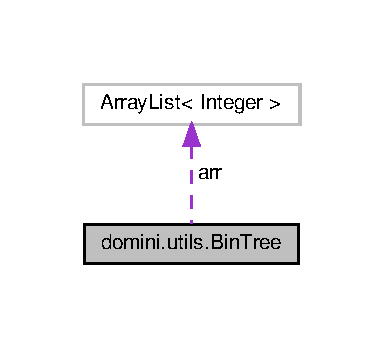
\includegraphics[width=184pt]{classdomini_1_1utils_1_1BinTree__coll__graph}
\end{center}
\end{figure}
\subsection*{Public Member Functions}
\begin{DoxyCompactItemize}
\item 
\mbox{\Hypertarget{classdomini_1_1utils_1_1BinTree_a83904c6ebf931ba29a134be5f29a66c7}\label{classdomini_1_1utils_1_1BinTree_a83904c6ebf931ba29a134be5f29a66c7}} 
{\bfseries Bin\+Tree} (int data)
\item 
\mbox{\Hypertarget{classdomini_1_1utils_1_1BinTree_a742c520d5bff9a17a4cd56d833aa62c0}\label{classdomini_1_1utils_1_1BinTree_a742c520d5bff9a17a4cd56d833aa62c0}} 
boolean {\bfseries well\+Defined} ()
\item 
\mbox{\Hypertarget{classdomini_1_1utils_1_1BinTree_a08e528b0f5bbebe0a5382be7f8e73a55}\label{classdomini_1_1utils_1_1BinTree_a08e528b0f5bbebe0a5382be7f8e73a55}} 
int {\bfseries size} ()
\item 
\mbox{\Hypertarget{classdomini_1_1utils_1_1BinTree_a6be9277eaecc3750a8aedfa045f8142b}\label{classdomini_1_1utils_1_1BinTree_a6be9277eaecc3750a8aedfa045f8142b}} 
boolean {\bfseries is\+Init} (int x)
\item 
\mbox{\Hypertarget{classdomini_1_1utils_1_1BinTree_a52ea101b3e66d5389a2350e6c777c517}\label{classdomini_1_1utils_1_1BinTree_a52ea101b3e66d5389a2350e6c777c517}} 
boolean {\bfseries is\+Leaf} (int x)
\item 
\mbox{\Hypertarget{classdomini_1_1utils_1_1BinTree_a256937f5412ac463258c67b8190708ba}\label{classdomini_1_1utils_1_1BinTree_a256937f5412ac463258c67b8190708ba}} 
int {\bfseries get\+Data} (int x)
\item 
\mbox{\Hypertarget{classdomini_1_1utils_1_1BinTree_a35dbfcf3a00a10d46240ce6295d4454c}\label{classdomini_1_1utils_1_1BinTree_a35dbfcf3a00a10d46240ce6295d4454c}} 
void {\bfseries set\+Data} (int x, int data)
\item 
\mbox{\Hypertarget{classdomini_1_1utils_1_1BinTree_ab44a6f728b74f5b3f0bd583d858de57e}\label{classdomini_1_1utils_1_1BinTree_ab44a6f728b74f5b3f0bd583d858de57e}} 
int {\bfseries get\+Child} (int x, int left\+\_\+right)
\item 
\mbox{\Hypertarget{classdomini_1_1utils_1_1BinTree_a8efc5cd06c9e5bad98ab7da0bc72c1cf}\label{classdomini_1_1utils_1_1BinTree_a8efc5cd06c9e5bad98ab7da0bc72c1cf}} 
int {\bfseries set\+Child} (int x, int left\+\_\+right, \hyperlink{classdomini_1_1utils_1_1BinTree}{Bin\+Tree} child)
\item 
\mbox{\Hypertarget{classdomini_1_1utils_1_1BinTree_ad8f921ac94ebe2a1007ed41b935099b1}\label{classdomini_1_1utils_1_1BinTree_ad8f921ac94ebe2a1007ed41b935099b1}} 
void {\bfseries print} ()
\end{DoxyCompactItemize}
\subsection*{Private Member Functions}
\begin{DoxyCompactItemize}
\item 
\mbox{\Hypertarget{classdomini_1_1utils_1_1BinTree_ae9ac7c25f515a2f89772406f01b769d2}\label{classdomini_1_1utils_1_1BinTree_ae9ac7c25f515a2f89772406f01b769d2}} 
void {\bfseries check\+Node} (int x)
\item 
\mbox{\Hypertarget{classdomini_1_1utils_1_1BinTree_ae65e589ea90a85ed18bba6bc9f74e9a2}\label{classdomini_1_1utils_1_1BinTree_ae65e589ea90a85ed18bba6bc9f74e9a2}} 
void {\bfseries print\+\_\+v2} (int tabs, int x)
\item 
\mbox{\Hypertarget{classdomini_1_1utils_1_1BinTree_a47c913594a3116b2e602c87fa4afc5c3}\label{classdomini_1_1utils_1_1BinTree_a47c913594a3116b2e602c87fa4afc5c3}} 
void {\bfseries print} (int tabs, int x)
\item 
\mbox{\Hypertarget{classdomini_1_1utils_1_1BinTree_aec1bd291bf3703915a815d09cfb0caf1}\label{classdomini_1_1utils_1_1BinTree_aec1bd291bf3703915a815d09cfb0caf1}} 
void {\bfseries print\+\_\+arr} ()
\end{DoxyCompactItemize}
\subsection*{Private Attributes}
\begin{DoxyCompactItemize}
\item 
Array\+List$<$ Integer $>$ \hyperlink{classdomini_1_1utils_1_1BinTree_a357bcbcf07ba7fcb99d11b237d189e65}{arr}
\item 
\mbox{\Hypertarget{classdomini_1_1utils_1_1BinTree_a36f1212262c353accbc0a0385fa45a8d}\label{classdomini_1_1utils_1_1BinTree_a36f1212262c353accbc0a0385fa45a8d}} 
int {\bfseries num\+\_\+undefs}
\end{DoxyCompactItemize}


\subsection{Member Data Documentation}
\mbox{\Hypertarget{classdomini_1_1utils_1_1BinTree_a357bcbcf07ba7fcb99d11b237d189e65}\label{classdomini_1_1utils_1_1BinTree_a357bcbcf07ba7fcb99d11b237d189e65}} 
\index{domini\+::utils\+::\+Bin\+Tree@{domini\+::utils\+::\+Bin\+Tree}!arr@{arr}}
\index{arr@{arr}!domini\+::utils\+::\+Bin\+Tree@{domini\+::utils\+::\+Bin\+Tree}}
\subsubsection{\texorpdfstring{arr}{arr}}
{\footnotesize\ttfamily Array\+List$<$Integer$>$ domini.\+utils.\+Bin\+Tree.\+arr\hspace{0.3cm}{\ttfamily [private]}}

Permet expressar arbres binaris on les fulles poden prendre valors enters. Els nodes s\textquotesingle{}identifiquen amb enters. Aquesta estroctura de dades permet afegir informació però no permet eliminar o modificar informació prèviament afegida, sigui x un node si arr\mbox{[}2$\ast$x\mbox{]} = -\/2, x és una fulla i arr\mbox{[}2$\ast$x+1\mbox{]} és el valor de x altrament x+arr\mbox{[}2$\ast$x\mbox{]} i x+arr\mbox{[}2$\ast$x+1\mbox{]} són els fills de x (-\/1 significa indefinit) Un node no està inicialitzat $<$-\/$>$ els dos fills son indefinits El node arrel és 0 

The documentation for this class was generated from the following file\+:\begin{DoxyCompactItemize}
\item 
src/domini/utils/Bin\+Tree.\+java\end{DoxyCompactItemize}

\hypertarget{classdomini_1_1utils_1_1byteToConversion}{}\section{domini.\+utils.\+byte\+To\+Conversion Class Reference}
\label{classdomini_1_1utils_1_1byteToConversion}\index{domini.\+utils.\+byte\+To\+Conversion@{domini.\+utils.\+byte\+To\+Conversion}}


Classe \hyperlink{classdomini_1_1utils_1_1byteToConversion}{byte\+To\+Conversion}.  


\subsection*{Static Public Member Functions}
\begin{DoxyCompactItemize}
\item 
static Character \hyperlink{classdomini_1_1utils_1_1byteToConversion_a5d2f5f8de52e4001cf6698ca03fe31e8}{byte\+To\+Character} (Byte b)
\begin{DoxyCompactList}\small\item\em Transforma un byte a Character. \end{DoxyCompactList}\item 
static Integer \hyperlink{classdomini_1_1utils_1_1byteToConversion_a3242a47adade49b6cfa6a9232944f587}{byte\+To\+Integer} (List$<$ Byte $>$ b\+Arg)
\begin{DoxyCompactList}\small\item\em Transforma un Array de bytes a un Enter. \end{DoxyCompactList}\item 
static byte \hyperlink{classdomini_1_1utils_1_1byteToConversion_a0e232cb9d272ccc13accda58bab9f8e1}{shift\+\_\+right\+\_\+logic} (byte b, int despl)
\begin{DoxyCompactList}\small\item\em Desplaçament lògic cap a la detra d\textquotesingle{}un byte. \end{DoxyCompactList}\end{DoxyCompactItemize}


\subsection{Detailed Description}
Classe \hyperlink{classdomini_1_1utils_1_1byteToConversion}{byte\+To\+Conversion}. 

\begin{DoxyAuthor}{Author}
Joan Bellavista 
\end{DoxyAuthor}


\subsection{Member Function Documentation}
\mbox{\Hypertarget{classdomini_1_1utils_1_1byteToConversion_a5d2f5f8de52e4001cf6698ca03fe31e8}\label{classdomini_1_1utils_1_1byteToConversion_a5d2f5f8de52e4001cf6698ca03fe31e8}} 
\index{domini\+::utils\+::byte\+To\+Conversion@{domini\+::utils\+::byte\+To\+Conversion}!byte\+To\+Character@{byte\+To\+Character}}
\index{byte\+To\+Character@{byte\+To\+Character}!domini\+::utils\+::byte\+To\+Conversion@{domini\+::utils\+::byte\+To\+Conversion}}
\subsubsection{\texorpdfstring{byte\+To\+Character()}{byteToCharacter()}}
{\footnotesize\ttfamily public static Character domini.\+utils.\+byte\+To\+Conversion.\+byte\+To\+Character (\begin{DoxyParamCaption}\item[{Byte}]{b }\end{DoxyParamCaption})\hspace{0.3cm}{\ttfamily [inline]}, {\ttfamily [static]}}



Transforma un byte a Character. 


\begin{DoxyParams}{Parameters}
{\em b} & Byte a transformar \\
\hline
\end{DoxyParams}
\begin{DoxyReturn}{Returns}
Character resultat de la transformació 
\end{DoxyReturn}
\mbox{\Hypertarget{classdomini_1_1utils_1_1byteToConversion_a3242a47adade49b6cfa6a9232944f587}\label{classdomini_1_1utils_1_1byteToConversion_a3242a47adade49b6cfa6a9232944f587}} 
\index{domini\+::utils\+::byte\+To\+Conversion@{domini\+::utils\+::byte\+To\+Conversion}!byte\+To\+Integer@{byte\+To\+Integer}}
\index{byte\+To\+Integer@{byte\+To\+Integer}!domini\+::utils\+::byte\+To\+Conversion@{domini\+::utils\+::byte\+To\+Conversion}}
\subsubsection{\texorpdfstring{byte\+To\+Integer()}{byteToInteger()}}
{\footnotesize\ttfamily public static Integer domini.\+utils.\+byte\+To\+Conversion.\+byte\+To\+Integer (\begin{DoxyParamCaption}\item[{List$<$ Byte $>$}]{b\+Arg }\end{DoxyParamCaption})\hspace{0.3cm}{\ttfamily [inline]}, {\ttfamily [static]}}



Transforma un Array de bytes a un Enter. 


\begin{DoxyParams}{Parameters}
{\em b\+Arg} & Llista de bytes que volem transformar \\
\hline
\end{DoxyParams}
\begin{DoxyReturn}{Returns}
Integer resultat de la conversió 
\end{DoxyReturn}
\mbox{\Hypertarget{classdomini_1_1utils_1_1byteToConversion_a0e232cb9d272ccc13accda58bab9f8e1}\label{classdomini_1_1utils_1_1byteToConversion_a0e232cb9d272ccc13accda58bab9f8e1}} 
\index{domini\+::utils\+::byte\+To\+Conversion@{domini\+::utils\+::byte\+To\+Conversion}!shift\+\_\+right\+\_\+logic@{shift\+\_\+right\+\_\+logic}}
\index{shift\+\_\+right\+\_\+logic@{shift\+\_\+right\+\_\+logic}!domini\+::utils\+::byte\+To\+Conversion@{domini\+::utils\+::byte\+To\+Conversion}}
\subsubsection{\texorpdfstring{shift\+\_\+right\+\_\+logic()}{shift\_right\_logic()}}
{\footnotesize\ttfamily public static byte domini.\+utils.\+byte\+To\+Conversion.\+shift\+\_\+right\+\_\+logic (\begin{DoxyParamCaption}\item[{byte}]{b,  }\item[{int}]{despl }\end{DoxyParamCaption})\hspace{0.3cm}{\ttfamily [inline]}, {\ttfamily [static]}}



Desplaçament lògic cap a la detra d\textquotesingle{}un byte. 


\begin{DoxyParams}{Parameters}
{\em b} & Byte que volem desplaçar \\
\hline
{\em despl} & Nombre de bits que volem desplaçar \\
\hline
\end{DoxyParams}
\begin{DoxyReturn}{Returns}
Byte desplaçat 
\end{DoxyReturn}


The documentation for this class was generated from the following file\+:\begin{DoxyCompactItemize}
\item 
src/domini/utils/\hyperlink{byteToConversion_8java}{byte\+To\+Conversion.\+java}\end{DoxyCompactItemize}

\hypertarget{classdomini_1_1algorithm_1_1Ctrl__Algorithm}{}\section{domini.\+algorithm.\+Ctrl\+\_\+\+Algorithm Class Reference}
\label{classdomini_1_1algorithm_1_1Ctrl__Algorithm}\index{domini.\+algorithm.\+Ctrl\+\_\+\+Algorithm@{domini.\+algorithm.\+Ctrl\+\_\+\+Algorithm}}


Classe de \hyperlink{classdomini_1_1algorithm_1_1Ctrl__Algorithm}{Ctrl\+\_\+\+Algorithm}.  


\subsection*{Public Member Functions}
\begin{DoxyCompactItemize}
\item 
\mbox{\Hypertarget{classdomini_1_1algorithm_1_1Ctrl__Algorithm_aa625781819b57512a3e42df15a3b2ffb}\label{classdomini_1_1algorithm_1_1Ctrl__Algorithm_aa625781819b57512a3e42df15a3b2ffb}} 
\hyperlink{classdomini_1_1algorithm_1_1Ctrl__Algorithm_aa625781819b57512a3e42df15a3b2ffb}{Ctrl\+\_\+\+Algorithm} ()
\begin{DoxyCompactList}\small\item\em Constructor de la classe. \end{DoxyCompactList}\item 
String \hyperlink{classdomini_1_1algorithm_1_1Ctrl__Algorithm_a5af3b3afa4465c95093532396cecb8c7}{Choose\+\_\+\+Encoder} (String Path, String method)
\begin{DoxyCompactList}\small\item\em Realitzar? la compressi? d\textquotesingle{}un fitxer segons un algoritme concret. \end{DoxyCompactList}\item 
String \hyperlink{classdomini_1_1algorithm_1_1Ctrl__Algorithm_a6f7a706e07d4e6f8c1ea293d06e17318}{Auto\+\_\+\+Encoder} (String Path)
\begin{DoxyCompactList}\small\item\em Determina de manera autom?tica quin compressor utilitzar. \end{DoxyCompactList}\item 
String \hyperlink{classdomini_1_1algorithm_1_1Ctrl__Algorithm_a613d15cc5326fc688b11d2c71ec9500a}{Auto\+\_\+\+Decoder} (String Path, String method)
\begin{DoxyCompactList}\small\item\em Escull de manera autom?tica quin descompressor emprar. \end{DoxyCompactList}\end{DoxyCompactItemize}


\subsection{Detailed Description}
Classe de \hyperlink{classdomini_1_1algorithm_1_1Ctrl__Algorithm}{Ctrl\+\_\+\+Algorithm}. 

\begin{DoxyAuthor}{Author}

\end{DoxyAuthor}


\subsection{Member Function Documentation}
\mbox{\Hypertarget{classdomini_1_1algorithm_1_1Ctrl__Algorithm_a613d15cc5326fc688b11d2c71ec9500a}\label{classdomini_1_1algorithm_1_1Ctrl__Algorithm_a613d15cc5326fc688b11d2c71ec9500a}} 
\index{domini\+::algorithm\+::\+Ctrl\+\_\+\+Algorithm@{domini\+::algorithm\+::\+Ctrl\+\_\+\+Algorithm}!Auto\+\_\+\+Decoder@{Auto\+\_\+\+Decoder}}
\index{Auto\+\_\+\+Decoder@{Auto\+\_\+\+Decoder}!domini\+::algorithm\+::\+Ctrl\+\_\+\+Algorithm@{domini\+::algorithm\+::\+Ctrl\+\_\+\+Algorithm}}
\subsubsection{\texorpdfstring{Auto\+\_\+\+Decoder()}{Auto\_Decoder()}}
{\footnotesize\ttfamily public String domini.\+algorithm.\+Ctrl\+\_\+\+Algorithm.\+Auto\+\_\+\+Decoder (\begin{DoxyParamCaption}\item[{String}]{Path,  }\item[{String}]{method }\end{DoxyParamCaption})\hspace{0.3cm}{\ttfamily [inline]}}



Escull de manera autom?tica quin descompressor emprar. 


\begin{DoxyParams}{Parameters}
{\em Path} & Path de l\textquotesingle{}arxiu a descomprimir \\
\hline
{\em method} & Descompressor a emprar \\
\hline
\end{DoxyParams}
\begin{DoxyReturn}{Returns}
Informaci? sobre la descompressio 
\end{DoxyReturn}
\mbox{\Hypertarget{classdomini_1_1algorithm_1_1Ctrl__Algorithm_a6f7a706e07d4e6f8c1ea293d06e17318}\label{classdomini_1_1algorithm_1_1Ctrl__Algorithm_a6f7a706e07d4e6f8c1ea293d06e17318}} 
\index{domini\+::algorithm\+::\+Ctrl\+\_\+\+Algorithm@{domini\+::algorithm\+::\+Ctrl\+\_\+\+Algorithm}!Auto\+\_\+\+Encoder@{Auto\+\_\+\+Encoder}}
\index{Auto\+\_\+\+Encoder@{Auto\+\_\+\+Encoder}!domini\+::algorithm\+::\+Ctrl\+\_\+\+Algorithm@{domini\+::algorithm\+::\+Ctrl\+\_\+\+Algorithm}}
\subsubsection{\texorpdfstring{Auto\+\_\+\+Encoder()}{Auto\_Encoder()}}
{\footnotesize\ttfamily public String domini.\+algorithm.\+Ctrl\+\_\+\+Algorithm.\+Auto\+\_\+\+Encoder (\begin{DoxyParamCaption}\item[{String}]{Path }\end{DoxyParamCaption})\hspace{0.3cm}{\ttfamily [inline]}}



Determina de manera autom?tica quin compressor utilitzar. 


\begin{DoxyParams}{Parameters}
{\em Path} & Path de l\textquotesingle{}arxiu a comprimir \\
\hline
\end{DoxyParams}
\begin{DoxyReturn}{Returns}
Nom del m?tode a emprar 
\end{DoxyReturn}
\mbox{\Hypertarget{classdomini_1_1algorithm_1_1Ctrl__Algorithm_a5af3b3afa4465c95093532396cecb8c7}\label{classdomini_1_1algorithm_1_1Ctrl__Algorithm_a5af3b3afa4465c95093532396cecb8c7}} 
\index{domini\+::algorithm\+::\+Ctrl\+\_\+\+Algorithm@{domini\+::algorithm\+::\+Ctrl\+\_\+\+Algorithm}!Choose\+\_\+\+Encoder@{Choose\+\_\+\+Encoder}}
\index{Choose\+\_\+\+Encoder@{Choose\+\_\+\+Encoder}!domini\+::algorithm\+::\+Ctrl\+\_\+\+Algorithm@{domini\+::algorithm\+::\+Ctrl\+\_\+\+Algorithm}}
\subsubsection{\texorpdfstring{Choose\+\_\+\+Encoder()}{Choose\_Encoder()}}
{\footnotesize\ttfamily public String domini.\+algorithm.\+Ctrl\+\_\+\+Algorithm.\+Choose\+\_\+\+Encoder (\begin{DoxyParamCaption}\item[{String}]{Path,  }\item[{String}]{method }\end{DoxyParamCaption})\hspace{0.3cm}{\ttfamily [inline]}}



Realitzar? la compressi? d\textquotesingle{}un fitxer segons un algoritme concret. 


\begin{DoxyParams}{Parameters}
{\em Path} & Path de l\textquotesingle{}arxiu a comprimir \\
\hline
{\em method} & Algoritme a emprar \\
\hline
\end{DoxyParams}
\begin{DoxyReturn}{Returns}
Informacio sobre la compressio 
\end{DoxyReturn}


The documentation for this class was generated from the following file\+:\begin{DoxyCompactItemize}
\item 
src/domini/algorithm/Ctrl\+\_\+\+Algorithm.\+java\end{DoxyCompactItemize}

\hypertarget{classpersistencia_1_1input_1_1Ctrl__Input}{}\section{persistencia.\+input.\+Ctrl\+\_\+\+Input Class Reference}
\label{classpersistencia_1_1input_1_1Ctrl__Input}\index{persistencia.\+input.\+Ctrl\+\_\+\+Input@{persistencia.\+input.\+Ctrl\+\_\+\+Input}}


Classe de \hyperlink{classpersistencia_1_1input_1_1Ctrl__Input}{Ctrl\+\_\+\+Input}.  




Inheritance diagram for persistencia.\+input.\+Ctrl\+\_\+\+Input\+:\nopagebreak
\begin{figure}[H]
\begin{center}
\leavevmode
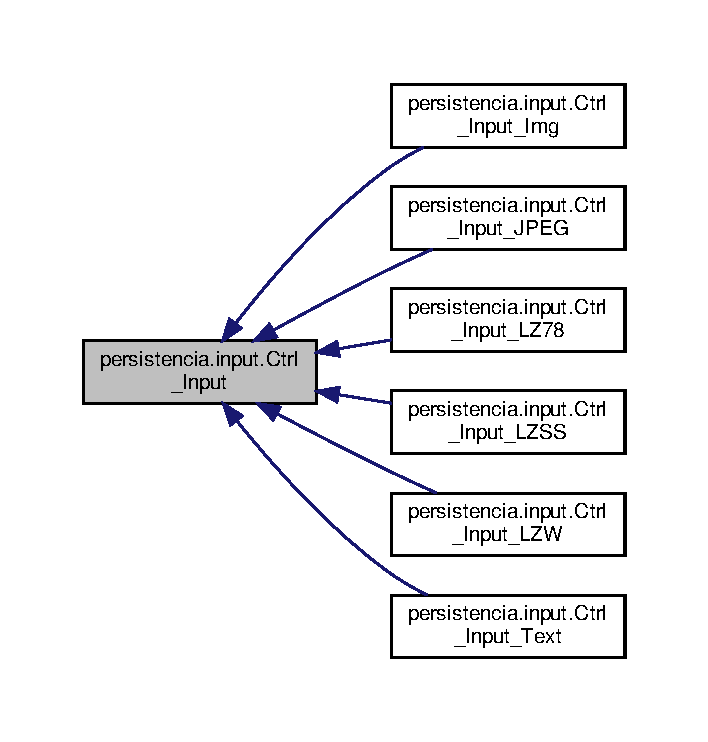
\includegraphics[width=340pt]{classpersistencia_1_1input_1_1Ctrl__Input__inherit__graph}
\end{center}
\end{figure}


Collaboration diagram for persistencia.\+input.\+Ctrl\+\_\+\+Input\+:
\nopagebreak
\begin{figure}[H]
\begin{center}
\leavevmode
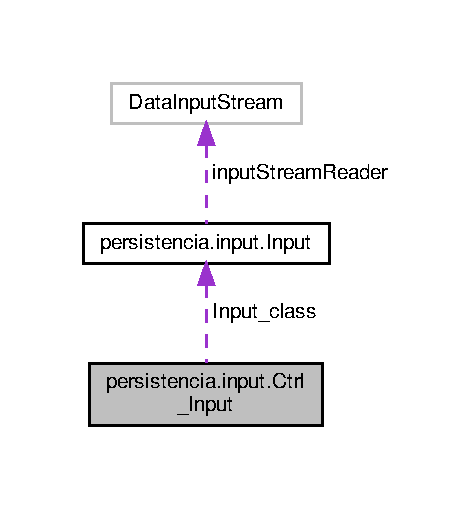
\includegraphics[width=227pt]{classpersistencia_1_1input_1_1Ctrl__Input__coll__graph}
\end{center}
\end{figure}
\subsection*{Public Member Functions}
\begin{DoxyCompactItemize}
\item 
\hyperlink{classpersistencia_1_1input_1_1Ctrl__Input_a00f3fa14d0329d6e4b9ddbe39ada1258}{Ctrl\+\_\+\+Input} (String path)
\begin{DoxyCompactList}\small\item\em Constructor de la classe. \end{DoxyCompactList}\item 
String \hyperlink{classpersistencia_1_1input_1_1Ctrl__Input_a46d569c2f3ceb0ab6cf9900708b3316a}{get\+Extension} ()
\item 
boolean \hyperlink{classpersistencia_1_1input_1_1Ctrl__Input_a5a94d207dce0fd592b5ac17f55154d4f}{finished} ()
\item 
String \hyperlink{classpersistencia_1_1input_1_1Ctrl__Input_aa69f79fb581f6d80c5a9609148794570}{get\+Alg} ()
\item 
\mbox{\Hypertarget{classpersistencia_1_1input_1_1Ctrl__Input_a46e05fce164a6803820c02565c1769c8}\label{classpersistencia_1_1input_1_1Ctrl__Input_a46e05fce164a6803820c02565c1769c8}} 
void \hyperlink{classpersistencia_1_1input_1_1Ctrl__Input_a46e05fce164a6803820c02565c1769c8}{get\+Metadata} ()
\begin{DoxyCompactList}\small\item\em Llegeix el dos primers bits de l\textquotesingle{}arxiu comprimit per saber amb quin algoritme ha sigut tractat. \end{DoxyCompactList}\end{DoxyCompactItemize}
\subsection*{Protected Attributes}
\begin{DoxyCompactItemize}
\item 
\hyperlink{classpersistencia_1_1input_1_1Input}{Input} \hyperlink{classpersistencia_1_1input_1_1Ctrl__Input_affe3c91673d80b61450970a69fe84611}{Input\+\_\+class}
\end{DoxyCompactItemize}
\subsection*{Package Attributes}
\begin{DoxyCompactItemize}
\item 
String \hyperlink{classpersistencia_1_1input_1_1Ctrl__Input_a6041b56aa31f01f75d02382f98e259e5}{Extensio}
\end{DoxyCompactItemize}


\subsection{Detailed Description}
Classe de \hyperlink{classpersistencia_1_1input_1_1Ctrl__Input}{Ctrl\+\_\+\+Input}. 

\begin{DoxyAuthor}{Author}

\end{DoxyAuthor}


\subsection{Constructor \& Destructor Documentation}
\mbox{\Hypertarget{classpersistencia_1_1input_1_1Ctrl__Input_a00f3fa14d0329d6e4b9ddbe39ada1258}\label{classpersistencia_1_1input_1_1Ctrl__Input_a00f3fa14d0329d6e4b9ddbe39ada1258}} 
\index{persistencia\+::input\+::\+Ctrl\+\_\+\+Input@{persistencia\+::input\+::\+Ctrl\+\_\+\+Input}!Ctrl\+\_\+\+Input@{Ctrl\+\_\+\+Input}}
\index{Ctrl\+\_\+\+Input@{Ctrl\+\_\+\+Input}!persistencia\+::input\+::\+Ctrl\+\_\+\+Input@{persistencia\+::input\+::\+Ctrl\+\_\+\+Input}}
\subsubsection{\texorpdfstring{Ctrl\+\_\+\+Input()}{Ctrl\_Input()}}
{\footnotesize\ttfamily persistencia.\+input.\+Ctrl\+\_\+\+Input.\+Ctrl\+\_\+\+Input (\begin{DoxyParamCaption}\item[{String}]{path }\end{DoxyParamCaption})\hspace{0.3cm}{\ttfamily [inline]}}



Constructor de la classe. 


\begin{DoxyParams}{Parameters}
{\em path} & Path de l\textquotesingle{}arxiu a tractar \\
\hline
\end{DoxyParams}


\subsection{Member Function Documentation}
\mbox{\Hypertarget{classpersistencia_1_1input_1_1Ctrl__Input_a5a94d207dce0fd592b5ac17f55154d4f}\label{classpersistencia_1_1input_1_1Ctrl__Input_a5a94d207dce0fd592b5ac17f55154d4f}} 
\index{persistencia\+::input\+::\+Ctrl\+\_\+\+Input@{persistencia\+::input\+::\+Ctrl\+\_\+\+Input}!finished@{finished}}
\index{finished@{finished}!persistencia\+::input\+::\+Ctrl\+\_\+\+Input@{persistencia\+::input\+::\+Ctrl\+\_\+\+Input}}
\subsubsection{\texorpdfstring{finished()}{finished()}}
{\footnotesize\ttfamily public boolean persistencia.\+input.\+Ctrl\+\_\+\+Input.\+finished (\begin{DoxyParamCaption}{ }\end{DoxyParamCaption})\hspace{0.3cm}{\ttfamily [inline]}}

\begin{DoxyReturn}{Returns}
Retorna si hem acabat de llegir l\textquotesingle{}arxiu o no 
\end{DoxyReturn}
\mbox{\Hypertarget{classpersistencia_1_1input_1_1Ctrl__Input_aa69f79fb581f6d80c5a9609148794570}\label{classpersistencia_1_1input_1_1Ctrl__Input_aa69f79fb581f6d80c5a9609148794570}} 
\index{persistencia\+::input\+::\+Ctrl\+\_\+\+Input@{persistencia\+::input\+::\+Ctrl\+\_\+\+Input}!get\+Alg@{get\+Alg}}
\index{get\+Alg@{get\+Alg}!persistencia\+::input\+::\+Ctrl\+\_\+\+Input@{persistencia\+::input\+::\+Ctrl\+\_\+\+Input}}
\subsubsection{\texorpdfstring{get\+Alg()}{getAlg()}}
{\footnotesize\ttfamily public String persistencia.\+input.\+Ctrl\+\_\+\+Input.\+get\+Alg (\begin{DoxyParamCaption}{ }\end{DoxyParamCaption})\hspace{0.3cm}{\ttfamily [inline]}}

\begin{DoxyReturn}{Returns}
Proporciona el algoritme mes adient per tractar la descompressio 
\end{DoxyReturn}
\mbox{\Hypertarget{classpersistencia_1_1input_1_1Ctrl__Input_a46d569c2f3ceb0ab6cf9900708b3316a}\label{classpersistencia_1_1input_1_1Ctrl__Input_a46d569c2f3ceb0ab6cf9900708b3316a}} 
\index{persistencia\+::input\+::\+Ctrl\+\_\+\+Input@{persistencia\+::input\+::\+Ctrl\+\_\+\+Input}!get\+Extension@{get\+Extension}}
\index{get\+Extension@{get\+Extension}!persistencia\+::input\+::\+Ctrl\+\_\+\+Input@{persistencia\+::input\+::\+Ctrl\+\_\+\+Input}}
\subsubsection{\texorpdfstring{get\+Extension()}{getExtension()}}
{\footnotesize\ttfamily public String persistencia.\+input.\+Ctrl\+\_\+\+Input.\+get\+Extension (\begin{DoxyParamCaption}{ }\end{DoxyParamCaption})\hspace{0.3cm}{\ttfamily [inline]}}

\begin{DoxyReturn}{Returns}
Retorna l\textquotesingle{}extensio de l\textquotesingle{}arxiu 
\end{DoxyReturn}


\subsection{Member Data Documentation}
\mbox{\Hypertarget{classpersistencia_1_1input_1_1Ctrl__Input_a6041b56aa31f01f75d02382f98e259e5}\label{classpersistencia_1_1input_1_1Ctrl__Input_a6041b56aa31f01f75d02382f98e259e5}} 
\index{persistencia\+::input\+::\+Ctrl\+\_\+\+Input@{persistencia\+::input\+::\+Ctrl\+\_\+\+Input}!Extensio@{Extensio}}
\index{Extensio@{Extensio}!persistencia\+::input\+::\+Ctrl\+\_\+\+Input@{persistencia\+::input\+::\+Ctrl\+\_\+\+Input}}
\subsubsection{\texorpdfstring{Extensio}{Extensio}}
{\footnotesize\ttfamily String persistencia.\+input.\+Ctrl\+\_\+\+Input.\+Extensio\hspace{0.3cm}{\ttfamily [package]}}


\begin{DoxyParams}{Parameters}
{\em Extensio} & Extensio de l\textquotesingle{}arxiu que estem tractant \\
\hline
\end{DoxyParams}
\mbox{\Hypertarget{classpersistencia_1_1input_1_1Ctrl__Input_affe3c91673d80b61450970a69fe84611}\label{classpersistencia_1_1input_1_1Ctrl__Input_affe3c91673d80b61450970a69fe84611}} 
\index{persistencia\+::input\+::\+Ctrl\+\_\+\+Input@{persistencia\+::input\+::\+Ctrl\+\_\+\+Input}!Input\+\_\+class@{Input\+\_\+class}}
\index{Input\+\_\+class@{Input\+\_\+class}!persistencia\+::input\+::\+Ctrl\+\_\+\+Input@{persistencia\+::input\+::\+Ctrl\+\_\+\+Input}}
\subsubsection{\texorpdfstring{Input\+\_\+class}{Input\_class}}
{\footnotesize\ttfamily \hyperlink{classpersistencia_1_1input_1_1Input}{Input} persistencia.\+input.\+Ctrl\+\_\+\+Input.\+Input\+\_\+class\hspace{0.3cm}{\ttfamily [protected]}}


\begin{DoxyParams}{Parameters}
{\em Input\+\_\+class} & Classe \hyperlink{classpersistencia_1_1input_1_1Input}{Input} \\
\hline
\end{DoxyParams}


The documentation for this class was generated from the following file\+:\begin{DoxyCompactItemize}
\item 
src/persistencia/input/Ctrl\+\_\+\+Input.\+java\end{DoxyCompactItemize}

\hypertarget{classpersistencia_1_1input_1_1Ctrl__Input__Img}{}\section{persistencia.\+input.\+Ctrl\+\_\+\+Input\+\_\+\+Img Class Reference}
\label{classpersistencia_1_1input_1_1Ctrl__Input__Img}\index{persistencia.\+input.\+Ctrl\+\_\+\+Input\+\_\+\+Img@{persistencia.\+input.\+Ctrl\+\_\+\+Input\+\_\+\+Img}}


Inheritance diagram for persistencia.\+input.\+Ctrl\+\_\+\+Input\+\_\+\+Img\+:\nopagebreak
\begin{figure}[H]
\begin{center}
\leavevmode
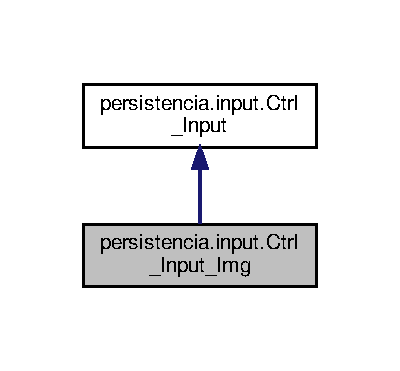
\includegraphics[width=192pt]{classpersistencia_1_1input_1_1Ctrl__Input__Img__inherit__graph}
\end{center}
\end{figure}


Collaboration diagram for persistencia.\+input.\+Ctrl\+\_\+\+Input\+\_\+\+Img\+:
\nopagebreak
\begin{figure}[H]
\begin{center}
\leavevmode
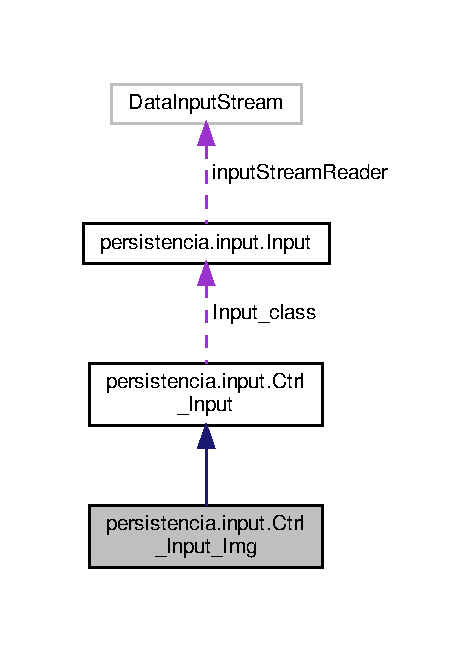
\includegraphics[width=227pt]{classpersistencia_1_1input_1_1Ctrl__Input__Img__coll__graph}
\end{center}
\end{figure}
\subsection*{Public Member Functions}
\begin{DoxyCompactItemize}
\item 
\mbox{\Hypertarget{classpersistencia_1_1input_1_1Ctrl__Input__Img_a79318a62df31dfd107554e92e29f6d9a}\label{classpersistencia_1_1input_1_1Ctrl__Input__Img_a79318a62df31dfd107554e92e29f6d9a}} 
{\bfseries Ctrl\+\_\+\+Input\+\_\+\+Img} (String path)
\item 
\mbox{\Hypertarget{classpersistencia_1_1input_1_1Ctrl__Input__Img_a27e92d786d8f11ce165780984122ac8f}\label{classpersistencia_1_1input_1_1Ctrl__Input__Img_a27e92d786d8f11ce165780984122ac8f}} 
int {\bfseries get\+Height} ()
\item 
\mbox{\Hypertarget{classpersistencia_1_1input_1_1Ctrl__Input__Img_a4ceade2796ead750824c89f2a1e6dc47}\label{classpersistencia_1_1input_1_1Ctrl__Input__Img_a4ceade2796ead750824c89f2a1e6dc47}} 
int {\bfseries get\+Width} ()
\item 
\mbox{\Hypertarget{classpersistencia_1_1input_1_1Ctrl__Input__Img_ac549527b5947a7ec9f40d53e492f4ffa}\label{classpersistencia_1_1input_1_1Ctrl__Input__Img_ac549527b5947a7ec9f40d53e492f4ffa}} 
double \mbox{[}$\,$\mbox{]}\mbox{[}$\,$\mbox{]}\mbox{[}$\,$\mbox{]}\mbox{[}$\,$\mbox{]} {\bfseries get} ()
\end{DoxyCompactItemize}
\subsection*{Package Attributes}
\begin{DoxyCompactItemize}
\item 
\mbox{\Hypertarget{classpersistencia_1_1input_1_1Ctrl__Input__Img_a1b8fa2d000a1d5d873be62d1f609e4be}\label{classpersistencia_1_1input_1_1Ctrl__Input__Img_a1b8fa2d000a1d5d873be62d1f609e4be}} 
int {\bfseries max\+\_\+val}
\item 
\mbox{\Hypertarget{classpersistencia_1_1input_1_1Ctrl__Input__Img_abc1dcc48714e9e74fb8ae0e0b81f91bf}\label{classpersistencia_1_1input_1_1Ctrl__Input__Img_abc1dcc48714e9e74fb8ae0e0b81f91bf}} 
int {\bfseries height}
\item 
\mbox{\Hypertarget{classpersistencia_1_1input_1_1Ctrl__Input__Img_a51dd0b9243b854aa25ac4532acca4524}\label{classpersistencia_1_1input_1_1Ctrl__Input__Img_a51dd0b9243b854aa25ac4532acca4524}} 
int {\bfseries width}
\item 
\mbox{\Hypertarget{classpersistencia_1_1input_1_1Ctrl__Input__Img_a222ad0e7d241e5f396cf67c3b760f143}\label{classpersistencia_1_1input_1_1Ctrl__Input__Img_a222ad0e7d241e5f396cf67c3b760f143}} 
int {\bfseries bits\+\_\+per\+\_\+val}
\end{DoxyCompactItemize}
\subsection*{Private Member Functions}
\begin{DoxyCompactItemize}
\item 
\mbox{\Hypertarget{classpersistencia_1_1input_1_1Ctrl__Input__Img_a6a4bdb0d78c8e25e0782a71875b5e541}\label{classpersistencia_1_1input_1_1Ctrl__Input__Img_a6a4bdb0d78c8e25e0782a71875b5e541}} 
char {\bfseries get\+Char} ()
\item 
\mbox{\Hypertarget{classpersistencia_1_1input_1_1Ctrl__Input__Img_a4219a110d7d84e7b883ffd88e18a0def}\label{classpersistencia_1_1input_1_1Ctrl__Input__Img_a4219a110d7d84e7b883ffd88e18a0def}} 
String {\bfseries get\+Word} ()
\item 
\mbox{\Hypertarget{classpersistencia_1_1input_1_1Ctrl__Input__Img_a430158ff229038ddc3476d406239f4cd}\label{classpersistencia_1_1input_1_1Ctrl__Input__Img_a430158ff229038ddc3476d406239f4cd}} 
int {\bfseries get\+Int\+A\+S\+C\+II} ()
\end{DoxyCompactItemize}
\subsection*{Additional Inherited Members}


The documentation for this class was generated from the following file\+:\begin{DoxyCompactItemize}
\item 
src/persistencia/input/Ctrl\+\_\+\+Input\+\_\+\+Img.\+java\end{DoxyCompactItemize}

\hypertarget{classpersistencia_1_1input_1_1Ctrl__Input__JPEG}{}\section{persistencia.\+input.\+Ctrl\+\_\+\+Input\+\_\+\+J\+P\+EG Class Reference}
\label{classpersistencia_1_1input_1_1Ctrl__Input__JPEG}\index{persistencia.\+input.\+Ctrl\+\_\+\+Input\+\_\+\+J\+P\+EG@{persistencia.\+input.\+Ctrl\+\_\+\+Input\+\_\+\+J\+P\+EG}}


Classe \hyperlink{classpersistencia_1_1input_1_1Ctrl__Input__JPEG}{Ctrl\+\_\+\+Input\+\_\+\+J\+P\+EG}.  




Inheritance diagram for persistencia.\+input.\+Ctrl\+\_\+\+Input\+\_\+\+J\+P\+EG\+:\nopagebreak
\begin{figure}[H]
\begin{center}
\leavevmode
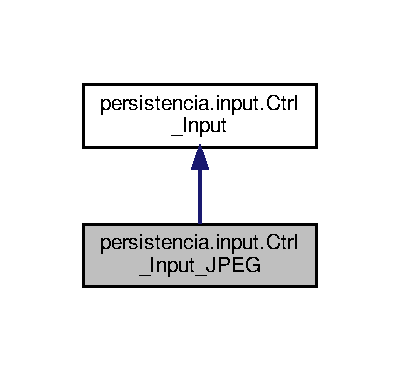
\includegraphics[width=192pt]{classpersistencia_1_1input_1_1Ctrl__Input__JPEG__inherit__graph}
\end{center}
\end{figure}


Collaboration diagram for persistencia.\+input.\+Ctrl\+\_\+\+Input\+\_\+\+J\+P\+EG\+:\nopagebreak
\begin{figure}[H]
\begin{center}
\leavevmode
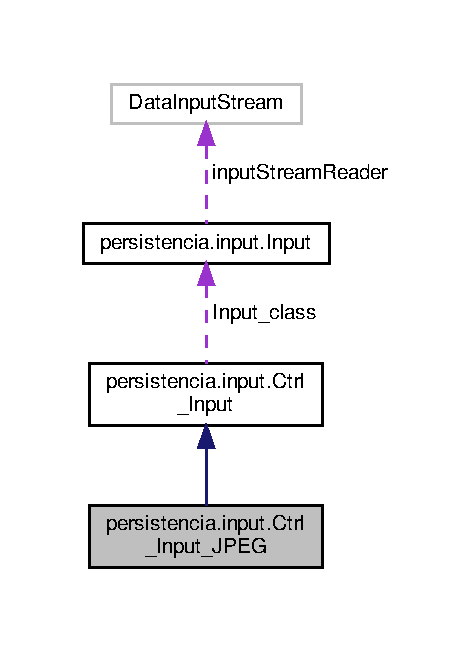
\includegraphics[width=227pt]{classpersistencia_1_1input_1_1Ctrl__Input__JPEG__coll__graph}
\end{center}
\end{figure}
\subsection*{Public Member Functions}
\begin{DoxyCompactItemize}
\item 
\hyperlink{classpersistencia_1_1input_1_1Ctrl__Input__JPEG_aa7d81dfa6240a7ee82e5188fc2600c58}{Ctrl\+\_\+\+Input\+\_\+\+J\+P\+EG} (String path)
\begin{DoxyCompactList}\small\item\em Constructor de la classe. \end{DoxyCompactList}\item 
\hyperlink{classpersistencia_1_1input_1_1Ctrl__Input__JPEG_a5c340483ee0fc78f985bd5d2ddcbb3a0}{Ctrl\+\_\+\+Input\+\_\+\+J\+P\+EG} ()
\begin{DoxyCompactList}\small\item\em Constructor de la classe. \end{DoxyCompactList}\item 
int \hyperlink{classpersistencia_1_1input_1_1Ctrl__Input__JPEG_a173716ac8d17365965ede95f99a8e65a}{get\+Height} ()
\begin{DoxyCompactList}\small\item\em Retorna l\textquotesingle{}alçada de la imatge. \end{DoxyCompactList}\item 
int \hyperlink{classpersistencia_1_1input_1_1Ctrl__Input__JPEG_ab4cd4c26db5bd1ce89f6e53458c99ba8}{get\+Width} ()
\begin{DoxyCompactList}\small\item\em Retorna l\textquotesingle{}amplada de la imatge. \end{DoxyCompactList}\item 
int \hyperlink{classpersistencia_1_1input_1_1Ctrl__Input__JPEG_a7c07d70b1dd3881e3322e9e3403e2ae7}{get\+Max\+Val} ()
\begin{DoxyCompactList}\small\item\em Retorna el valor màxim que poden prendre els enters que representan quantitat de color en la imatge ppm orignial. \end{DoxyCompactList}\item 
int \hyperlink{classpersistencia_1_1input_1_1Ctrl__Input__JPEG_a702b13d096ba57f06b242987f0dbf4ec}{get} (int size)
\end{DoxyCompactItemize}
\subsection*{Package Attributes}
\begin{DoxyCompactItemize}
\item 
int \hyperlink{classpersistencia_1_1input_1_1Ctrl__Input__JPEG_a9e6805b998e58981f8cd7b8b6e609f27}{height}
\item 
int \hyperlink{classpersistencia_1_1input_1_1Ctrl__Input__JPEG_a07d902b25b54941dc0444398c7d380e7}{width}
\item 
int \hyperlink{classpersistencia_1_1input_1_1Ctrl__Input__JPEG_a8720235be6a11ef90085217064bbb1b0}{max\+\_\+val}
\end{DoxyCompactItemize}
\subsection*{Additional Inherited Members}


\subsection{Detailed Description}
Classe \hyperlink{classpersistencia_1_1input_1_1Ctrl__Input__JPEG}{Ctrl\+\_\+\+Input\+\_\+\+J\+P\+EG}. 

\subsection{Constructor \& Destructor Documentation}
\mbox{\Hypertarget{classpersistencia_1_1input_1_1Ctrl__Input__JPEG_aa7d81dfa6240a7ee82e5188fc2600c58}\label{classpersistencia_1_1input_1_1Ctrl__Input__JPEG_aa7d81dfa6240a7ee82e5188fc2600c58}} 
\index{persistencia\+::input\+::\+Ctrl\+\_\+\+Input\+\_\+\+J\+P\+EG@{persistencia\+::input\+::\+Ctrl\+\_\+\+Input\+\_\+\+J\+P\+EG}!Ctrl\+\_\+\+Input\+\_\+\+J\+P\+EG@{Ctrl\+\_\+\+Input\+\_\+\+J\+P\+EG}}
\index{Ctrl\+\_\+\+Input\+\_\+\+J\+P\+EG@{Ctrl\+\_\+\+Input\+\_\+\+J\+P\+EG}!persistencia\+::input\+::\+Ctrl\+\_\+\+Input\+\_\+\+J\+P\+EG@{persistencia\+::input\+::\+Ctrl\+\_\+\+Input\+\_\+\+J\+P\+EG}}
\subsubsection{\texorpdfstring{Ctrl\+\_\+\+Input\+\_\+\+J\+P\+E\+G()}{Ctrl\_Input\_JPEG()}\hspace{0.1cm}{\footnotesize\ttfamily [1/2]}}
{\footnotesize\ttfamily persistencia.\+input.\+Ctrl\+\_\+\+Input\+\_\+\+J\+P\+E\+G.\+Ctrl\+\_\+\+Input\+\_\+\+J\+P\+EG (\begin{DoxyParamCaption}\item[{String}]{path }\end{DoxyParamCaption})\hspace{0.3cm}{\ttfamily [inline]}}



Constructor de la classe. 


\begin{DoxyParams}{Parameters}
{\em path} & Path de l\textquotesingle{}arxiu que comença a lelgir. \\
\hline
\end{DoxyParams}

\begin{DoxyCode}
29                                         \{
30         super(path);
31         \hyperlink{classpersistencia_1_1input_1_1Ctrl__Input_a46e05fce164a6803820c02565c1769c8}{getMetadata}();
32         \hyperlink{classpersistencia_1_1input_1_1Ctrl__Input__JPEG_a07d902b25b54941dc0444398c7d380e7}{width} = \textcolor{keyword}{get}(32);
33         \hyperlink{classpersistencia_1_1input_1_1Ctrl__Input__JPEG_a9e6805b998e58981f8cd7b8b6e609f27}{height} = \textcolor{keyword}{get}(32);
34         \hyperlink{classpersistencia_1_1input_1_1Ctrl__Input__JPEG_a8720235be6a11ef90085217064bbb1b0}{max\_val} = \textcolor{keyword}{get}(32);
35     \}
\end{DoxyCode}
\mbox{\Hypertarget{classpersistencia_1_1input_1_1Ctrl__Input__JPEG_a5c340483ee0fc78f985bd5d2ddcbb3a0}\label{classpersistencia_1_1input_1_1Ctrl__Input__JPEG_a5c340483ee0fc78f985bd5d2ddcbb3a0}} 
\index{persistencia\+::input\+::\+Ctrl\+\_\+\+Input\+\_\+\+J\+P\+EG@{persistencia\+::input\+::\+Ctrl\+\_\+\+Input\+\_\+\+J\+P\+EG}!Ctrl\+\_\+\+Input\+\_\+\+J\+P\+EG@{Ctrl\+\_\+\+Input\+\_\+\+J\+P\+EG}}
\index{Ctrl\+\_\+\+Input\+\_\+\+J\+P\+EG@{Ctrl\+\_\+\+Input\+\_\+\+J\+P\+EG}!persistencia\+::input\+::\+Ctrl\+\_\+\+Input\+\_\+\+J\+P\+EG@{persistencia\+::input\+::\+Ctrl\+\_\+\+Input\+\_\+\+J\+P\+EG}}
\subsubsection{\texorpdfstring{Ctrl\+\_\+\+Input\+\_\+\+J\+P\+E\+G()}{Ctrl\_Input\_JPEG()}\hspace{0.1cm}{\footnotesize\ttfamily [2/2]}}
{\footnotesize\ttfamily persistencia.\+input.\+Ctrl\+\_\+\+Input\+\_\+\+J\+P\+E\+G.\+Ctrl\+\_\+\+Input\+\_\+\+J\+P\+EG (\begin{DoxyParamCaption}{ }\end{DoxyParamCaption})\hspace{0.3cm}{\ttfamily [inline]}}



Constructor de la classe. 

\begin{DoxyNote}{Note}
Continua llegint el fitxer que s\textquotesingle{}estava llegint. Assumeix que la metadata ja ha estat llegida. 
\end{DoxyNote}

\begin{DoxyCode}
41                              \{
42         super();
43         \hyperlink{classpersistencia_1_1input_1_1Ctrl__Input__JPEG_a07d902b25b54941dc0444398c7d380e7}{width} = \textcolor{keyword}{get}(32);
44         \hyperlink{classpersistencia_1_1input_1_1Ctrl__Input__JPEG_a9e6805b998e58981f8cd7b8b6e609f27}{height} = \textcolor{keyword}{get}(32);
45         \hyperlink{classpersistencia_1_1input_1_1Ctrl__Input__JPEG_a8720235be6a11ef90085217064bbb1b0}{max\_val} = \textcolor{keyword}{get}(32);
46     \}
\end{DoxyCode}


\subsection{Member Function Documentation}
\mbox{\Hypertarget{classpersistencia_1_1input_1_1Ctrl__Input__JPEG_a702b13d096ba57f06b242987f0dbf4ec}\label{classpersistencia_1_1input_1_1Ctrl__Input__JPEG_a702b13d096ba57f06b242987f0dbf4ec}} 
\index{persistencia\+::input\+::\+Ctrl\+\_\+\+Input\+\_\+\+J\+P\+EG@{persistencia\+::input\+::\+Ctrl\+\_\+\+Input\+\_\+\+J\+P\+EG}!get@{get}}
\index{get@{get}!persistencia\+::input\+::\+Ctrl\+\_\+\+Input\+\_\+\+J\+P\+EG@{persistencia\+::input\+::\+Ctrl\+\_\+\+Input\+\_\+\+J\+P\+EG}}
\subsubsection{\texorpdfstring{get()}{get()}}
{\footnotesize\ttfamily public int persistencia.\+input.\+Ctrl\+\_\+\+Input\+\_\+\+J\+P\+E\+G.\+get (\begin{DoxyParamCaption}\item[{int}]{size }\end{DoxyParamCaption})\hspace{0.3cm}{\ttfamily [inline]}}

llageix \textquotesingle{}size\textquotesingle{} bits \begin{DoxyReturn}{Returns}
Retorna els bits llegits en forma de int. Els primers bits llegits son els menys significatius. 
\end{DoxyReturn}

\begin{DoxyCode}
80                              \{
81         \textcolor{keywordflow}{if} (size == 0) \textcolor{keywordflow}{return} 0;
82         \textcolor{keywordtype}{int} sz;
83         \textcolor{keywordflow}{if} (size < 8) sz = size;
84         \textcolor{keywordflow}{else} sz = 8;
85 
86         \textcolor{keywordtype}{int} x = ((int)Input.getInstance().getBits(sz)) & ~(0xffffffff << sz);
87         \textcolor{keywordflow}{if} (size > 8) x = x + (\textcolor{keyword}{get}(size-8) << 8);
88         \textcolor{keywordflow}{return} x;
89     \}
\end{DoxyCode}
\mbox{\Hypertarget{classpersistencia_1_1input_1_1Ctrl__Input__JPEG_a173716ac8d17365965ede95f99a8e65a}\label{classpersistencia_1_1input_1_1Ctrl__Input__JPEG_a173716ac8d17365965ede95f99a8e65a}} 
\index{persistencia\+::input\+::\+Ctrl\+\_\+\+Input\+\_\+\+J\+P\+EG@{persistencia\+::input\+::\+Ctrl\+\_\+\+Input\+\_\+\+J\+P\+EG}!get\+Height@{get\+Height}}
\index{get\+Height@{get\+Height}!persistencia\+::input\+::\+Ctrl\+\_\+\+Input\+\_\+\+J\+P\+EG@{persistencia\+::input\+::\+Ctrl\+\_\+\+Input\+\_\+\+J\+P\+EG}}
\subsubsection{\texorpdfstring{get\+Height()}{getHeight()}}
{\footnotesize\ttfamily public int persistencia.\+input.\+Ctrl\+\_\+\+Input\+\_\+\+J\+P\+E\+G.\+get\+Height (\begin{DoxyParamCaption}{ }\end{DoxyParamCaption})\hspace{0.3cm}{\ttfamily [inline]}}



Retorna l\textquotesingle{}alçada de la imatge. 

\begin{DoxyReturn}{Returns}
Alçada 
\end{DoxyReturn}

\begin{DoxyCode}
53                            \{
54         \textcolor{keywordflow}{return} \hyperlink{classpersistencia_1_1input_1_1Ctrl__Input__JPEG_a9e6805b998e58981f8cd7b8b6e609f27}{height};
55     \}
\end{DoxyCode}
\mbox{\Hypertarget{classpersistencia_1_1input_1_1Ctrl__Input__JPEG_a7c07d70b1dd3881e3322e9e3403e2ae7}\label{classpersistencia_1_1input_1_1Ctrl__Input__JPEG_a7c07d70b1dd3881e3322e9e3403e2ae7}} 
\index{persistencia\+::input\+::\+Ctrl\+\_\+\+Input\+\_\+\+J\+P\+EG@{persistencia\+::input\+::\+Ctrl\+\_\+\+Input\+\_\+\+J\+P\+EG}!get\+Max\+Val@{get\+Max\+Val}}
\index{get\+Max\+Val@{get\+Max\+Val}!persistencia\+::input\+::\+Ctrl\+\_\+\+Input\+\_\+\+J\+P\+EG@{persistencia\+::input\+::\+Ctrl\+\_\+\+Input\+\_\+\+J\+P\+EG}}
\subsubsection{\texorpdfstring{get\+Max\+Val()}{getMaxVal()}}
{\footnotesize\ttfamily public int persistencia.\+input.\+Ctrl\+\_\+\+Input\+\_\+\+J\+P\+E\+G.\+get\+Max\+Val (\begin{DoxyParamCaption}{ }\end{DoxyParamCaption})\hspace{0.3cm}{\ttfamily [inline]}}



Retorna el valor màxim que poden prendre els enters que representan quantitat de color en la imatge ppm orignial. 

\begin{DoxyReturn}{Returns}
Valor màxim que poden prendre els enters que representan quantitat de color. 
\end{DoxyReturn}

\begin{DoxyCode}
70                            \{
71         \textcolor{keywordflow}{return} \hyperlink{classpersistencia_1_1input_1_1Ctrl__Input__JPEG_a8720235be6a11ef90085217064bbb1b0}{max\_val};
72     \}
\end{DoxyCode}
\mbox{\Hypertarget{classpersistencia_1_1input_1_1Ctrl__Input__JPEG_ab4cd4c26db5bd1ce89f6e53458c99ba8}\label{classpersistencia_1_1input_1_1Ctrl__Input__JPEG_ab4cd4c26db5bd1ce89f6e53458c99ba8}} 
\index{persistencia\+::input\+::\+Ctrl\+\_\+\+Input\+\_\+\+J\+P\+EG@{persistencia\+::input\+::\+Ctrl\+\_\+\+Input\+\_\+\+J\+P\+EG}!get\+Width@{get\+Width}}
\index{get\+Width@{get\+Width}!persistencia\+::input\+::\+Ctrl\+\_\+\+Input\+\_\+\+J\+P\+EG@{persistencia\+::input\+::\+Ctrl\+\_\+\+Input\+\_\+\+J\+P\+EG}}
\subsubsection{\texorpdfstring{get\+Width()}{getWidth()}}
{\footnotesize\ttfamily public int persistencia.\+input.\+Ctrl\+\_\+\+Input\+\_\+\+J\+P\+E\+G.\+get\+Width (\begin{DoxyParamCaption}{ }\end{DoxyParamCaption})\hspace{0.3cm}{\ttfamily [inline]}}



Retorna l\textquotesingle{}amplada de la imatge. 

\begin{DoxyReturn}{Returns}
Amplada 
\end{DoxyReturn}

\begin{DoxyCode}
61                           \{
62         \textcolor{keywordflow}{return} \hyperlink{classpersistencia_1_1input_1_1Ctrl__Input__JPEG_a07d902b25b54941dc0444398c7d380e7}{width};
63     \}
\end{DoxyCode}


\subsection{Member Data Documentation}
\mbox{\Hypertarget{classpersistencia_1_1input_1_1Ctrl__Input__JPEG_a9e6805b998e58981f8cd7b8b6e609f27}\label{classpersistencia_1_1input_1_1Ctrl__Input__JPEG_a9e6805b998e58981f8cd7b8b6e609f27}} 
\index{persistencia\+::input\+::\+Ctrl\+\_\+\+Input\+\_\+\+J\+P\+EG@{persistencia\+::input\+::\+Ctrl\+\_\+\+Input\+\_\+\+J\+P\+EG}!height@{height}}
\index{height@{height}!persistencia\+::input\+::\+Ctrl\+\_\+\+Input\+\_\+\+J\+P\+EG@{persistencia\+::input\+::\+Ctrl\+\_\+\+Input\+\_\+\+J\+P\+EG}}
\subsubsection{\texorpdfstring{height}{height}}
{\footnotesize\ttfamily int persistencia.\+input.\+Ctrl\+\_\+\+Input\+\_\+\+J\+P\+E\+G.\+height\hspace{0.3cm}{\ttfamily [package]}}


\begin{DoxyParams}{Parameters}
{\em height} & Alçada de la imatge \\
\hline
\end{DoxyParams}
\mbox{\Hypertarget{classpersistencia_1_1input_1_1Ctrl__Input__JPEG_a8720235be6a11ef90085217064bbb1b0}\label{classpersistencia_1_1input_1_1Ctrl__Input__JPEG_a8720235be6a11ef90085217064bbb1b0}} 
\index{persistencia\+::input\+::\+Ctrl\+\_\+\+Input\+\_\+\+J\+P\+EG@{persistencia\+::input\+::\+Ctrl\+\_\+\+Input\+\_\+\+J\+P\+EG}!max\+\_\+val@{max\+\_\+val}}
\index{max\+\_\+val@{max\+\_\+val}!persistencia\+::input\+::\+Ctrl\+\_\+\+Input\+\_\+\+J\+P\+EG@{persistencia\+::input\+::\+Ctrl\+\_\+\+Input\+\_\+\+J\+P\+EG}}
\subsubsection{\texorpdfstring{max\+\_\+val}{max\_val}}
{\footnotesize\ttfamily int persistencia.\+input.\+Ctrl\+\_\+\+Input\+\_\+\+J\+P\+E\+G.\+max\+\_\+val\hspace{0.3cm}{\ttfamily [package]}}


\begin{DoxyParams}{Parameters}
{\em max\+\_\+val} & Valor màxim que tenien els codis de color a la imatge original. \\
\hline
\end{DoxyParams}
\mbox{\Hypertarget{classpersistencia_1_1input_1_1Ctrl__Input__JPEG_a07d902b25b54941dc0444398c7d380e7}\label{classpersistencia_1_1input_1_1Ctrl__Input__JPEG_a07d902b25b54941dc0444398c7d380e7}} 
\index{persistencia\+::input\+::\+Ctrl\+\_\+\+Input\+\_\+\+J\+P\+EG@{persistencia\+::input\+::\+Ctrl\+\_\+\+Input\+\_\+\+J\+P\+EG}!width@{width}}
\index{width@{width}!persistencia\+::input\+::\+Ctrl\+\_\+\+Input\+\_\+\+J\+P\+EG@{persistencia\+::input\+::\+Ctrl\+\_\+\+Input\+\_\+\+J\+P\+EG}}
\subsubsection{\texorpdfstring{width}{width}}
{\footnotesize\ttfamily int persistencia.\+input.\+Ctrl\+\_\+\+Input\+\_\+\+J\+P\+E\+G.\+width\hspace{0.3cm}{\ttfamily [package]}}


\begin{DoxyParams}{Parameters}
{\em width} & Amplada de la imatge \\
\hline
\end{DoxyParams}


The documentation for this class was generated from the following file\+:\begin{DoxyCompactItemize}
\item 
src/persistencia/input/\hyperlink{Ctrl__Input__JPEG_8java}{Ctrl\+\_\+\+Input\+\_\+\+J\+P\+E\+G.\+java}\end{DoxyCompactItemize}

\hypertarget{classpersistencia_1_1input_1_1Ctrl__Input__LZ78}{}\section{persistencia.\+input.\+Ctrl\+\_\+\+Input\+\_\+\+L\+Z78 Class Reference}
\label{classpersistencia_1_1input_1_1Ctrl__Input__LZ78}\index{persistencia.\+input.\+Ctrl\+\_\+\+Input\+\_\+\+L\+Z78@{persistencia.\+input.\+Ctrl\+\_\+\+Input\+\_\+\+L\+Z78}}


Acces a un arxiu comprimit amb L\+Z78.  




Inheritance diagram for persistencia.\+input.\+Ctrl\+\_\+\+Input\+\_\+\+L\+Z78\+:\nopagebreak
\begin{figure}[H]
\begin{center}
\leavevmode
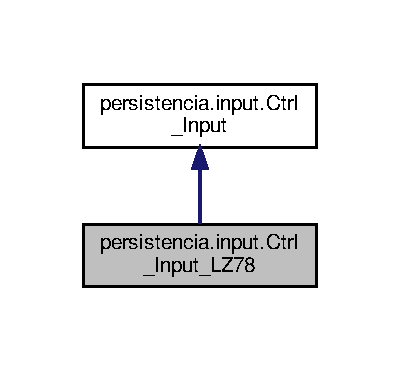
\includegraphics[width=192pt]{classpersistencia_1_1input_1_1Ctrl__Input__LZ78__inherit__graph}
\end{center}
\end{figure}


Collaboration diagram for persistencia.\+input.\+Ctrl\+\_\+\+Input\+\_\+\+L\+Z78\+:\nopagebreak
\begin{figure}[H]
\begin{center}
\leavevmode
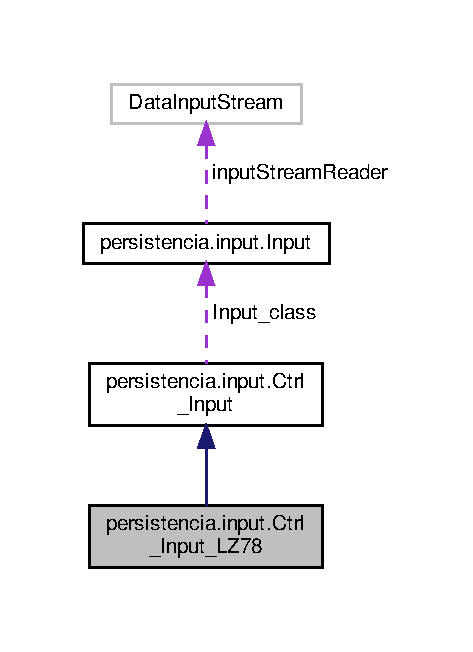
\includegraphics[width=227pt]{classpersistencia_1_1input_1_1Ctrl__Input__LZ78__coll__graph}
\end{center}
\end{figure}
\subsection*{Public Member Functions}
\begin{DoxyCompactItemize}
\item 
\hyperlink{classpersistencia_1_1input_1_1Ctrl__Input__LZ78_a3629302a8c1eb2b0c7367ad0ea542780}{Ctrl\+\_\+\+Input\+\_\+\+L\+Z78} (String path)
\begin{DoxyCompactList}\small\item\em Constructor de la classe. \end{DoxyCompactList}\item 
\hyperlink{classdomini_1_1utils_1_1Pair}{Pair}$<$ Integer, Byte $>$ \hyperlink{classpersistencia_1_1input_1_1Ctrl__Input__LZ78_ae09535962f284be3a76369845c15b78c}{get} ()
\end{DoxyCompactItemize}
\subsection*{Additional Inherited Members}


\subsection{Detailed Description}
Acces a un arxiu comprimit amb L\+Z78. 

\begin{DoxyAuthor}{Author}
Joan Bellavista Bartroli 
\end{DoxyAuthor}


\subsection{Constructor \& Destructor Documentation}
\mbox{\Hypertarget{classpersistencia_1_1input_1_1Ctrl__Input__LZ78_a3629302a8c1eb2b0c7367ad0ea542780}\label{classpersistencia_1_1input_1_1Ctrl__Input__LZ78_a3629302a8c1eb2b0c7367ad0ea542780}} 
\index{persistencia\+::input\+::\+Ctrl\+\_\+\+Input\+\_\+\+L\+Z78@{persistencia\+::input\+::\+Ctrl\+\_\+\+Input\+\_\+\+L\+Z78}!Ctrl\+\_\+\+Input\+\_\+\+L\+Z78@{Ctrl\+\_\+\+Input\+\_\+\+L\+Z78}}
\index{Ctrl\+\_\+\+Input\+\_\+\+L\+Z78@{Ctrl\+\_\+\+Input\+\_\+\+L\+Z78}!persistencia\+::input\+::\+Ctrl\+\_\+\+Input\+\_\+\+L\+Z78@{persistencia\+::input\+::\+Ctrl\+\_\+\+Input\+\_\+\+L\+Z78}}
\subsubsection{\texorpdfstring{Ctrl\+\_\+\+Input\+\_\+\+L\+Z78()}{Ctrl\_Input\_LZ78()}}
{\footnotesize\ttfamily persistencia.\+input.\+Ctrl\+\_\+\+Input\+\_\+\+L\+Z78.\+Ctrl\+\_\+\+Input\+\_\+\+L\+Z78 (\begin{DoxyParamCaption}\item[{String}]{path }\end{DoxyParamCaption})\hspace{0.3cm}{\ttfamily [inline]}}



Constructor de la classe. 


\begin{DoxyParams}{Parameters}
{\em path} & Path de l\textquotesingle{}arxiu comprimit \\
\hline
\end{DoxyParams}


\subsection{Member Function Documentation}
\mbox{\Hypertarget{classpersistencia_1_1input_1_1Ctrl__Input__LZ78_ae09535962f284be3a76369845c15b78c}\label{classpersistencia_1_1input_1_1Ctrl__Input__LZ78_ae09535962f284be3a76369845c15b78c}} 
\index{persistencia\+::input\+::\+Ctrl\+\_\+\+Input\+\_\+\+L\+Z78@{persistencia\+::input\+::\+Ctrl\+\_\+\+Input\+\_\+\+L\+Z78}!get@{get}}
\index{get@{get}!persistencia\+::input\+::\+Ctrl\+\_\+\+Input\+\_\+\+L\+Z78@{persistencia\+::input\+::\+Ctrl\+\_\+\+Input\+\_\+\+L\+Z78}}
\subsubsection{\texorpdfstring{get()}{get()}}
{\footnotesize\ttfamily public \hyperlink{classdomini_1_1utils_1_1Pair}{Pair}$<$ Integer, Character $>$ persistencia.\+input.\+Ctrl\+\_\+\+Input\+\_\+\+L\+Z78.\+get (\begin{DoxyParamCaption}{ }\end{DoxyParamCaption})\hspace{0.3cm}{\ttfamily [inline]}}

\begin{DoxyReturn}{Returns}
Primer enter no llegit de l\textquotesingle{}arxiu comprimit amb L\+Z78 
\end{DoxyReturn}


The documentation for this class was generated from the following file\+:\begin{DoxyCompactItemize}
\item 
src/persistencia/input/Ctrl\+\_\+\+Input\+\_\+\+L\+Z78.\+java\end{DoxyCompactItemize}

\hypertarget{classpersistencia_1_1input_1_1Ctrl__Input__LZSS}{}\section{persistencia.\+input.\+Ctrl\+\_\+\+Input\+\_\+\+L\+Z\+SS Class Reference}
\label{classpersistencia_1_1input_1_1Ctrl__Input__LZSS}\index{persistencia.\+input.\+Ctrl\+\_\+\+Input\+\_\+\+L\+Z\+SS@{persistencia.\+input.\+Ctrl\+\_\+\+Input\+\_\+\+L\+Z\+SS}}


Aquesta és la classe fill del controlador \hyperlink{classpersistencia_1_1input_1_1Ctrl__Input}{Ctrl\+\_\+\+Input}.  




Inheritance diagram for persistencia.\+input.\+Ctrl\+\_\+\+Input\+\_\+\+L\+Z\+SS\+:\nopagebreak
\begin{figure}[H]
\begin{center}
\leavevmode
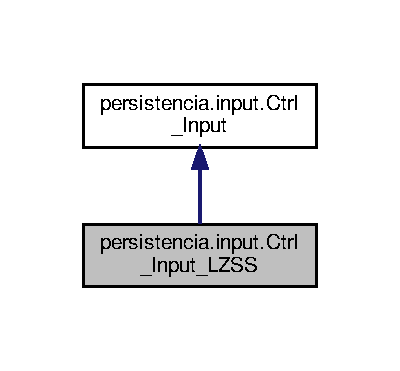
\includegraphics[width=192pt]{classpersistencia_1_1input_1_1Ctrl__Input__LZSS__inherit__graph}
\end{center}
\end{figure}


Collaboration diagram for persistencia.\+input.\+Ctrl\+\_\+\+Input\+\_\+\+L\+Z\+SS\+:\nopagebreak
\begin{figure}[H]
\begin{center}
\leavevmode
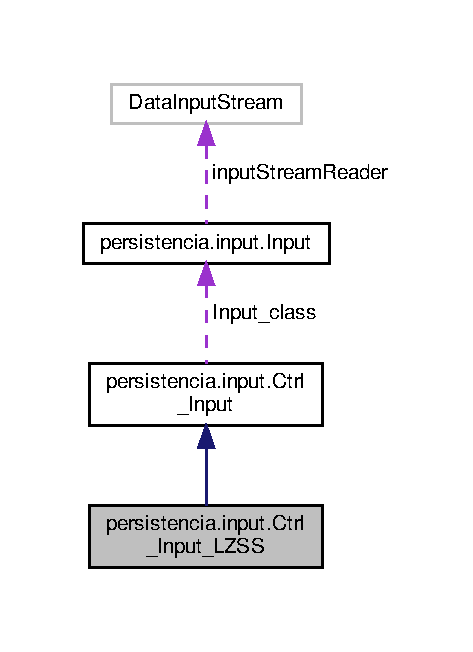
\includegraphics[width=227pt]{classpersistencia_1_1input_1_1Ctrl__Input__LZSS__coll__graph}
\end{center}
\end{figure}
\subsection*{Public Member Functions}
\begin{DoxyCompactItemize}
\item 
\hyperlink{classpersistencia_1_1input_1_1Ctrl__Input__LZSS_a00d5d178971cfd1d15604f97584368d5}{Ctrl\+\_\+\+Input\+\_\+\+L\+Z\+SS} (String path)
\begin{DoxyCompactList}\small\item\em El constructor on es crida a la classe pare. \end{DoxyCompactList}\item 
\hyperlink{classdomini_1_1utils_1_1IntorByte}{Intor\+Byte} \hyperlink{classpersistencia_1_1input_1_1Ctrl__Input__LZSS_a204d4d68a1d94725d9017b71bac0288e}{get\+L\+Z\+SS} ()
\begin{DoxyCompactList}\small\item\em Mètode per aconseguir la unitat mínima necessària. \end{DoxyCompactList}\end{DoxyCompactItemize}
\subsection*{Additional Inherited Members}


\subsection{Detailed Description}
Aquesta és la classe fill del controlador \hyperlink{classpersistencia_1_1input_1_1Ctrl__Input}{Ctrl\+\_\+\+Input}. 

Aquesta classe tracta d\textquotesingle{}obtenir la unitat mínima necessària per al input de l\textquotesingle{}algorisme L\+Z\+SS.

\begin{DoxyAuthor}{Author}
Manel Aguilar 
\end{DoxyAuthor}


\subsection{Constructor \& Destructor Documentation}
\mbox{\Hypertarget{classpersistencia_1_1input_1_1Ctrl__Input__LZSS_a00d5d178971cfd1d15604f97584368d5}\label{classpersistencia_1_1input_1_1Ctrl__Input__LZSS_a00d5d178971cfd1d15604f97584368d5}} 
\index{persistencia\+::input\+::\+Ctrl\+\_\+\+Input\+\_\+\+L\+Z\+SS@{persistencia\+::input\+::\+Ctrl\+\_\+\+Input\+\_\+\+L\+Z\+SS}!Ctrl\+\_\+\+Input\+\_\+\+L\+Z\+SS@{Ctrl\+\_\+\+Input\+\_\+\+L\+Z\+SS}}
\index{Ctrl\+\_\+\+Input\+\_\+\+L\+Z\+SS@{Ctrl\+\_\+\+Input\+\_\+\+L\+Z\+SS}!persistencia\+::input\+::\+Ctrl\+\_\+\+Input\+\_\+\+L\+Z\+SS@{persistencia\+::input\+::\+Ctrl\+\_\+\+Input\+\_\+\+L\+Z\+SS}}
\subsubsection{\texorpdfstring{Ctrl\+\_\+\+Input\+\_\+\+L\+Z\+S\+S()}{Ctrl\_Input\_LZSS()}}
{\footnotesize\ttfamily persistencia.\+input.\+Ctrl\+\_\+\+Input\+\_\+\+L\+Z\+S\+S.\+Ctrl\+\_\+\+Input\+\_\+\+L\+Z\+SS (\begin{DoxyParamCaption}\item[{String}]{path }\end{DoxyParamCaption})\hspace{0.3cm}{\ttfamily [inline]}}



El constructor on es crida a la classe pare. 


\begin{DoxyParams}{Parameters}
{\em path} & Conté el path del arxiu. \\
\hline
\end{DoxyParams}


\subsection{Member Function Documentation}
\mbox{\Hypertarget{classpersistencia_1_1input_1_1Ctrl__Input__LZSS_a204d4d68a1d94725d9017b71bac0288e}\label{classpersistencia_1_1input_1_1Ctrl__Input__LZSS_a204d4d68a1d94725d9017b71bac0288e}} 
\index{persistencia\+::input\+::\+Ctrl\+\_\+\+Input\+\_\+\+L\+Z\+SS@{persistencia\+::input\+::\+Ctrl\+\_\+\+Input\+\_\+\+L\+Z\+SS}!get\+L\+Z\+SS@{get\+L\+Z\+SS}}
\index{get\+L\+Z\+SS@{get\+L\+Z\+SS}!persistencia\+::input\+::\+Ctrl\+\_\+\+Input\+\_\+\+L\+Z\+SS@{persistencia\+::input\+::\+Ctrl\+\_\+\+Input\+\_\+\+L\+Z\+SS}}
\subsubsection{\texorpdfstring{get\+L\+Z\+S\+S()}{getLZSS()}}
{\footnotesize\ttfamily public \hyperlink{classdomini_1_1utils_1_1IntorByte}{Intor\+Byte} persistencia.\+input.\+Ctrl\+\_\+\+Input\+\_\+\+L\+Z\+S\+S.\+get\+L\+Z\+SS (\begin{DoxyParamCaption}{ }\end{DoxyParamCaption})\hspace{0.3cm}{\ttfamily [inline]}}



Mètode per aconseguir la unitat mínima necessària. 

\begin{DoxyReturn}{Returns}
Tracta d\textquotesingle{}obtenir o bé un Byte o bé dos Integers. 
\end{DoxyReturn}


The documentation for this class was generated from the following file\+:\begin{DoxyCompactItemize}
\item 
src/persistencia/input/\hyperlink{Ctrl__Input__LZSS_8java}{Ctrl\+\_\+\+Input\+\_\+\+L\+Z\+S\+S.\+java}\end{DoxyCompactItemize}

\hypertarget{classpersistencia_1_1input_1_1Ctrl__Input__LZW}{}\section{persistencia.\+input.\+Ctrl\+\_\+\+Input\+\_\+\+L\+ZW Class Reference}
\label{classpersistencia_1_1input_1_1Ctrl__Input__LZW}\index{persistencia.\+input.\+Ctrl\+\_\+\+Input\+\_\+\+L\+ZW@{persistencia.\+input.\+Ctrl\+\_\+\+Input\+\_\+\+L\+ZW}}


Acces a un arxiu comprimit amb L\+ZW.  




Inheritance diagram for persistencia.\+input.\+Ctrl\+\_\+\+Input\+\_\+\+L\+ZW\+:
\nopagebreak
\begin{figure}[H]
\begin{center}
\leavevmode
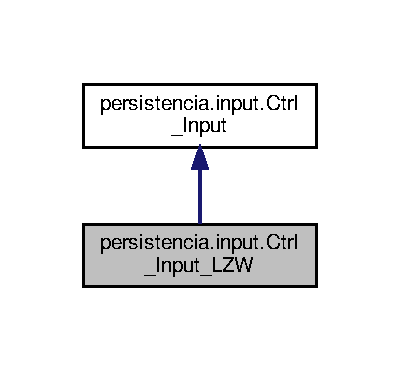
\includegraphics[width=192pt]{classpersistencia_1_1input_1_1Ctrl__Input__LZW__inherit__graph}
\end{center}
\end{figure}


Collaboration diagram for persistencia.\+input.\+Ctrl\+\_\+\+Input\+\_\+\+L\+ZW\+:
\nopagebreak
\begin{figure}[H]
\begin{center}
\leavevmode
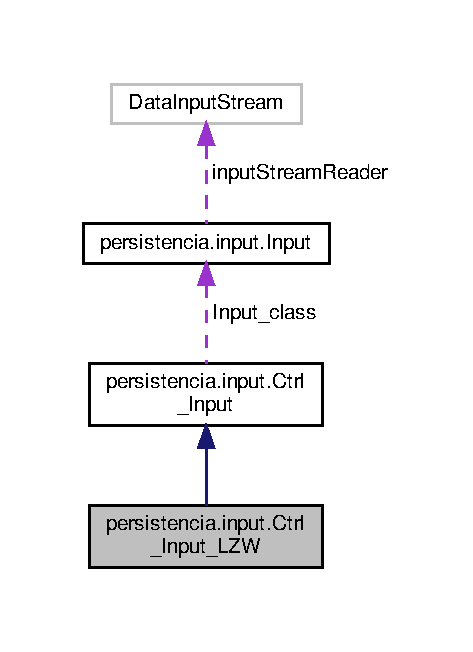
\includegraphics[width=198pt]{classpersistencia_1_1input_1_1Ctrl__Input__LZW__coll__graph}
\end{center}
\end{figure}
\subsection*{Public Member Functions}
\begin{DoxyCompactItemize}
\item 
\hyperlink{classpersistencia_1_1input_1_1Ctrl__Input__LZW_a31503f303ac443e110379322e851791a}{Ctrl\+\_\+\+Input\+\_\+\+L\+ZW} (String path)
\begin{DoxyCompactList}\small\item\em Constructor de la classe. \end{DoxyCompactList}\item 
Integer \hyperlink{classpersistencia_1_1input_1_1Ctrl__Input__LZW_a821592197863ec1b1f052a794753ea40}{get} ()
\end{DoxyCompactItemize}
\subsection*{Additional Inherited Members}


\subsection{Detailed Description}
Acces a un arxiu comprimit amb L\+ZW. 

\begin{DoxyAuthor}{Author}
Miguel Paracuellos Ocana 
\end{DoxyAuthor}


\subsection{Constructor \& Destructor Documentation}
\mbox{\Hypertarget{classpersistencia_1_1input_1_1Ctrl__Input__LZW_a31503f303ac443e110379322e851791a}\label{classpersistencia_1_1input_1_1Ctrl__Input__LZW_a31503f303ac443e110379322e851791a}} 
\index{persistencia\+::input\+::\+Ctrl\+\_\+\+Input\+\_\+\+L\+ZW@{persistencia\+::input\+::\+Ctrl\+\_\+\+Input\+\_\+\+L\+ZW}!Ctrl\+\_\+\+Input\+\_\+\+L\+ZW@{Ctrl\+\_\+\+Input\+\_\+\+L\+ZW}}
\index{Ctrl\+\_\+\+Input\+\_\+\+L\+ZW@{Ctrl\+\_\+\+Input\+\_\+\+L\+ZW}!persistencia\+::input\+::\+Ctrl\+\_\+\+Input\+\_\+\+L\+ZW@{persistencia\+::input\+::\+Ctrl\+\_\+\+Input\+\_\+\+L\+ZW}}
\subsubsection{\texorpdfstring{Ctrl\+\_\+\+Input\+\_\+\+L\+Z\+W()}{Ctrl\_Input\_LZW()}}
{\footnotesize\ttfamily persistencia.\+input.\+Ctrl\+\_\+\+Input\+\_\+\+L\+Z\+W.\+Ctrl\+\_\+\+Input\+\_\+\+L\+ZW (\begin{DoxyParamCaption}\item[{String}]{path }\end{DoxyParamCaption})\hspace{0.3cm}{\ttfamily [inline]}}



Constructor de la classe. 


\begin{DoxyParams}{Parameters}
{\em path} & Path de l\textquotesingle{}arxiu comprimit \\
\hline
\end{DoxyParams}


\subsection{Member Function Documentation}
\mbox{\Hypertarget{classpersistencia_1_1input_1_1Ctrl__Input__LZW_a821592197863ec1b1f052a794753ea40}\label{classpersistencia_1_1input_1_1Ctrl__Input__LZW_a821592197863ec1b1f052a794753ea40}} 
\index{persistencia\+::input\+::\+Ctrl\+\_\+\+Input\+\_\+\+L\+ZW@{persistencia\+::input\+::\+Ctrl\+\_\+\+Input\+\_\+\+L\+ZW}!get@{get}}
\index{get@{get}!persistencia\+::input\+::\+Ctrl\+\_\+\+Input\+\_\+\+L\+ZW@{persistencia\+::input\+::\+Ctrl\+\_\+\+Input\+\_\+\+L\+ZW}}
\subsubsection{\texorpdfstring{get()}{get()}}
{\footnotesize\ttfamily public Integer persistencia.\+input.\+Ctrl\+\_\+\+Input\+\_\+\+L\+Z\+W.\+get (\begin{DoxyParamCaption}{ }\end{DoxyParamCaption})\hspace{0.3cm}{\ttfamily [inline]}}

\begin{DoxyReturn}{Returns}
Primer enter no llegit de l\textquotesingle{}arxiu comprimit amb L\+ZW 
\end{DoxyReturn}


The documentation for this class was generated from the following file\+:\begin{DoxyCompactItemize}
\item 
src/persistencia/input/Ctrl\+\_\+\+Input\+\_\+\+L\+Z\+W.\+java\end{DoxyCompactItemize}

\hypertarget{classpersistencia_1_1input_1_1Ctrl__Input__Text}{}\section{persistencia.\+input.\+Ctrl\+\_\+\+Input\+\_\+\+Text Class Reference}
\label{classpersistencia_1_1input_1_1Ctrl__Input__Text}\index{persistencia.\+input.\+Ctrl\+\_\+\+Input\+\_\+\+Text@{persistencia.\+input.\+Ctrl\+\_\+\+Input\+\_\+\+Text}}


Classe de \hyperlink{classpersistencia_1_1input_1_1Ctrl__Input__Text}{Ctrl\+\_\+\+Input\+\_\+\+Text}.  




Inheritance diagram for persistencia.\+input.\+Ctrl\+\_\+\+Input\+\_\+\+Text\+:\nopagebreak
\begin{figure}[H]
\begin{center}
\leavevmode
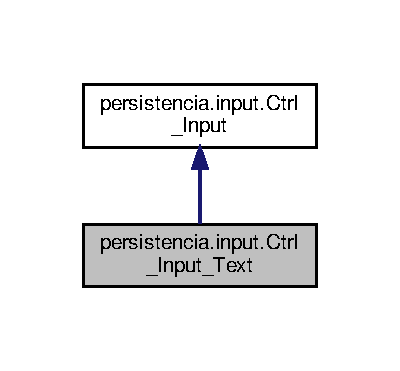
\includegraphics[width=192pt]{classpersistencia_1_1input_1_1Ctrl__Input__Text__inherit__graph}
\end{center}
\end{figure}


Collaboration diagram for persistencia.\+input.\+Ctrl\+\_\+\+Input\+\_\+\+Text\+:
\nopagebreak
\begin{figure}[H]
\begin{center}
\leavevmode
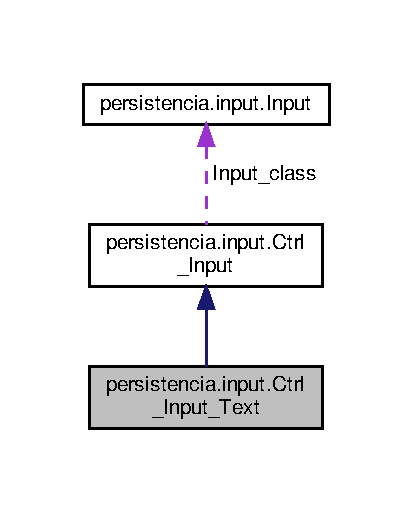
\includegraphics[width=227pt]{classpersistencia_1_1input_1_1Ctrl__Input__Text__coll__graph}
\end{center}
\end{figure}
\subsection*{Public Member Functions}
\begin{DoxyCompactItemize}
\item 
\hyperlink{classpersistencia_1_1input_1_1Ctrl__Input__Text_a945833e6bb2bb3fbdb328ae01392410f}{Ctrl\+\_\+\+Input\+\_\+\+Text} (String path)
\begin{DoxyCompactList}\small\item\em Constructor de la classe. \end{DoxyCompactList}\item 
byte \hyperlink{classpersistencia_1_1input_1_1Ctrl__Input__Text_a8b501ae723f8c6f8d63305a56e9720c3}{get} ()
\begin{DoxyCompactList}\small\item\em Proporciona el proxim byte a llegir. \end{DoxyCompactList}\end{DoxyCompactItemize}
\subsection*{Package Attributes}
\begin{DoxyCompactItemize}
\item 
byte \hyperlink{classpersistencia_1_1input_1_1Ctrl__Input__Text_a533e9e0497774114b57d8dd5a6bbb000}{seguent}
\end{DoxyCompactItemize}
\subsection*{Additional Inherited Members}


\subsection{Detailed Description}
Classe de \hyperlink{classpersistencia_1_1input_1_1Ctrl__Input__Text}{Ctrl\+\_\+\+Input\+\_\+\+Text}. 

\begin{DoxyAuthor}{Author}
Miguel Paracuellos 
\end{DoxyAuthor}


\subsection{Constructor \& Destructor Documentation}
\mbox{\Hypertarget{classpersistencia_1_1input_1_1Ctrl__Input__Text_a945833e6bb2bb3fbdb328ae01392410f}\label{classpersistencia_1_1input_1_1Ctrl__Input__Text_a945833e6bb2bb3fbdb328ae01392410f}} 
\index{persistencia\+::input\+::\+Ctrl\+\_\+\+Input\+\_\+\+Text@{persistencia\+::input\+::\+Ctrl\+\_\+\+Input\+\_\+\+Text}!Ctrl\+\_\+\+Input\+\_\+\+Text@{Ctrl\+\_\+\+Input\+\_\+\+Text}}
\index{Ctrl\+\_\+\+Input\+\_\+\+Text@{Ctrl\+\_\+\+Input\+\_\+\+Text}!persistencia\+::input\+::\+Ctrl\+\_\+\+Input\+\_\+\+Text@{persistencia\+::input\+::\+Ctrl\+\_\+\+Input\+\_\+\+Text}}
\subsubsection{\texorpdfstring{Ctrl\+\_\+\+Input\+\_\+\+Text()}{Ctrl\_Input\_Text()}}
{\footnotesize\ttfamily persistencia.\+input.\+Ctrl\+\_\+\+Input\+\_\+\+Text.\+Ctrl\+\_\+\+Input\+\_\+\+Text (\begin{DoxyParamCaption}\item[{String}]{path }\end{DoxyParamCaption})\hspace{0.3cm}{\ttfamily [inline]}}



Constructor de la classe. 


\begin{DoxyParams}{Parameters}
{\em path} & Path de l\textquotesingle{}arxiu input \\
\hline
\end{DoxyParams}


\subsection{Member Function Documentation}
\mbox{\Hypertarget{classpersistencia_1_1input_1_1Ctrl__Input__Text_a8b501ae723f8c6f8d63305a56e9720c3}\label{classpersistencia_1_1input_1_1Ctrl__Input__Text_a8b501ae723f8c6f8d63305a56e9720c3}} 
\index{persistencia\+::input\+::\+Ctrl\+\_\+\+Input\+\_\+\+Text@{persistencia\+::input\+::\+Ctrl\+\_\+\+Input\+\_\+\+Text}!get@{get}}
\index{get@{get}!persistencia\+::input\+::\+Ctrl\+\_\+\+Input\+\_\+\+Text@{persistencia\+::input\+::\+Ctrl\+\_\+\+Input\+\_\+\+Text}}
\subsubsection{\texorpdfstring{get()}{get()}}
{\footnotesize\ttfamily public byte persistencia.\+input.\+Ctrl\+\_\+\+Input\+\_\+\+Text.\+get (\begin{DoxyParamCaption}{ }\end{DoxyParamCaption})\hspace{0.3cm}{\ttfamily [inline]}}



Proporciona el proxim byte a llegir. 

\begin{DoxyNote}{Note}
Passa tots els caracters a codi A\+S\+C\+II 
\end{DoxyNote}
\begin{DoxyReturn}{Returns}
Retorna el proxim byte de l\textquotesingle{}arxiu, en el cas de que no haguem arribat al final 
\end{DoxyReturn}


\subsection{Member Data Documentation}
\mbox{\Hypertarget{classpersistencia_1_1input_1_1Ctrl__Input__Text_a533e9e0497774114b57d8dd5a6bbb000}\label{classpersistencia_1_1input_1_1Ctrl__Input__Text_a533e9e0497774114b57d8dd5a6bbb000}} 
\index{persistencia\+::input\+::\+Ctrl\+\_\+\+Input\+\_\+\+Text@{persistencia\+::input\+::\+Ctrl\+\_\+\+Input\+\_\+\+Text}!seguent@{seguent}}
\index{seguent@{seguent}!persistencia\+::input\+::\+Ctrl\+\_\+\+Input\+\_\+\+Text@{persistencia\+::input\+::\+Ctrl\+\_\+\+Input\+\_\+\+Text}}
\subsubsection{\texorpdfstring{seguent}{seguent}}
{\footnotesize\ttfamily byte persistencia.\+input.\+Ctrl\+\_\+\+Input\+\_\+\+Text.\+seguent\hspace{0.3cm}{\ttfamily [package]}}


\begin{DoxyParams}{Parameters}
{\em seguent} & Proper byte a llegir \\
\hline
\end{DoxyParams}


The documentation for this class was generated from the following file\+:\begin{DoxyCompactItemize}
\item 
src/persistencia/input/Ctrl\+\_\+\+Input\+\_\+\+Text.\+java\end{DoxyCompactItemize}

\hypertarget{classpresentacion_1_1master_1_1Ctrl__Master}{}\section{presentacion.\+master.\+Ctrl\+\_\+\+Master Class Reference}
\label{classpresentacion_1_1master_1_1Ctrl__Master}\index{presentacion.\+master.\+Ctrl\+\_\+\+Master@{presentacion.\+master.\+Ctrl\+\_\+\+Master}}


Classe \hyperlink{classpresentacion_1_1master_1_1Ctrl__Master}{Ctrl\+\_\+\+Master}.  


\subsection*{Public Member Functions}
\begin{DoxyCompactItemize}
\item 
\mbox{\Hypertarget{classpresentacion_1_1master_1_1Ctrl__Master_a7336c36d767f4eb13e75761b67de17c4}\label{classpresentacion_1_1master_1_1Ctrl__Master_a7336c36d767f4eb13e75761b67de17c4}} 
\hyperlink{classpresentacion_1_1master_1_1Ctrl__Master_a7336c36d767f4eb13e75761b67de17c4}{Ctrl\+\_\+\+Master} ()
\begin{DoxyCompactList}\small\item\em Constructor de la classe. \end{DoxyCompactList}\item 
\mbox{\Hypertarget{classpresentacion_1_1master_1_1Ctrl__Master_adf19ba4025da7654d5e7c01d9f5650c1}\label{classpresentacion_1_1master_1_1Ctrl__Master_adf19ba4025da7654d5e7c01d9f5650c1}} 
void \hyperlink{classpresentacion_1_1master_1_1Ctrl__Master_adf19ba4025da7654d5e7c01d9f5650c1}{Context} ()
\begin{DoxyCompactList}\small\item\em S\textquotesingle{}encarrega de preguntar a l\textquotesingle{}usuari que vol fer. \end{DoxyCompactList}\item 
String \hyperlink{classpresentacion_1_1master_1_1Ctrl__Master_aa25099e202de5e076b950e4e3bf5c26b}{Work} ()
\begin{DoxyCompactList}\small\item\em Realitza l\textquotesingle{}accio que l\textquotesingle{}usuari hagi indicar. \end{DoxyCompactList}\end{DoxyCompactItemize}
\subsection*{Package Attributes}
\begin{DoxyCompactItemize}
\item 
Integer \hyperlink{classpresentacion_1_1master_1_1Ctrl__Master_a5358a65f5f7bc39f860af1d858739d41}{Function}
\item 
String \hyperlink{classpresentacion_1_1master_1_1Ctrl__Master_a3d2cb29ead7034fa79496fca2da0157a}{Path}
\end{DoxyCompactItemize}


\subsection{Detailed Description}
Classe \hyperlink{classpresentacion_1_1master_1_1Ctrl__Master}{Ctrl\+\_\+\+Master}. 

\begin{DoxyAuthor}{Author}
Miguel Paracuellos 
\end{DoxyAuthor}


\subsection{Member Function Documentation}
\mbox{\Hypertarget{classpresentacion_1_1master_1_1Ctrl__Master_aa25099e202de5e076b950e4e3bf5c26b}\label{classpresentacion_1_1master_1_1Ctrl__Master_aa25099e202de5e076b950e4e3bf5c26b}} 
\index{presentacion\+::master\+::\+Ctrl\+\_\+\+Master@{presentacion\+::master\+::\+Ctrl\+\_\+\+Master}!Work@{Work}}
\index{Work@{Work}!presentacion\+::master\+::\+Ctrl\+\_\+\+Master@{presentacion\+::master\+::\+Ctrl\+\_\+\+Master}}
\subsubsection{\texorpdfstring{Work()}{Work()}}
{\footnotesize\ttfamily public String presentacion.\+master.\+Ctrl\+\_\+\+Master.\+Work (\begin{DoxyParamCaption}{ }\end{DoxyParamCaption})\hspace{0.3cm}{\ttfamily [inline]}}



Realitza l\textquotesingle{}accio que l\textquotesingle{}usuari hagi indicar. 

\begin{DoxyReturn}{Returns}
Retorna informació sobre l\textquotesingle{}execucio 
\end{DoxyReturn}


\subsection{Member Data Documentation}
\mbox{\Hypertarget{classpresentacion_1_1master_1_1Ctrl__Master_a5358a65f5f7bc39f860af1d858739d41}\label{classpresentacion_1_1master_1_1Ctrl__Master_a5358a65f5f7bc39f860af1d858739d41}} 
\index{presentacion\+::master\+::\+Ctrl\+\_\+\+Master@{presentacion\+::master\+::\+Ctrl\+\_\+\+Master}!Function@{Function}}
\index{Function@{Function}!presentacion\+::master\+::\+Ctrl\+\_\+\+Master@{presentacion\+::master\+::\+Ctrl\+\_\+\+Master}}
\subsubsection{\texorpdfstring{Function}{Function}}
{\footnotesize\ttfamily Integer presentacion.\+master.\+Ctrl\+\_\+\+Master.\+Function\hspace{0.3cm}{\ttfamily [package]}}


\begin{DoxyParams}{Parameters}
{\em Function} & Indica el que vol fer l\textquotesingle{}usuari \\
\hline
\end{DoxyParams}
\mbox{\Hypertarget{classpresentacion_1_1master_1_1Ctrl__Master_a3d2cb29ead7034fa79496fca2da0157a}\label{classpresentacion_1_1master_1_1Ctrl__Master_a3d2cb29ead7034fa79496fca2da0157a}} 
\index{presentacion\+::master\+::\+Ctrl\+\_\+\+Master@{presentacion\+::master\+::\+Ctrl\+\_\+\+Master}!Path@{Path}}
\index{Path@{Path}!presentacion\+::master\+::\+Ctrl\+\_\+\+Master@{presentacion\+::master\+::\+Ctrl\+\_\+\+Master}}
\subsubsection{\texorpdfstring{Path}{Path}}
{\footnotesize\ttfamily String presentacion.\+master.\+Ctrl\+\_\+\+Master.\+Path\hspace{0.3cm}{\ttfamily [package]}}


\begin{DoxyParams}{Parameters}
{\em Path} & Path de l\textquotesingle{}arxiu que hem de tractar \\
\hline
\end{DoxyParams}


The documentation for this class was generated from the following file\+:\begin{DoxyCompactItemize}
\item 
src/presentacion/master/Ctrl\+\_\+\+Master.\+java\end{DoxyCompactItemize}

\hypertarget{classpersistencia_1_1output_1_1Ctrl__Output}{}\section{persistencia.\+output.\+Ctrl\+\_\+\+Output Class Reference}
\label{classpersistencia_1_1output_1_1Ctrl__Output}\index{persistencia.\+output.\+Ctrl\+\_\+\+Output@{persistencia.\+output.\+Ctrl\+\_\+\+Output}}


Classe \hyperlink{classpersistencia_1_1output_1_1Ctrl__Output}{Ctrl\+\_\+\+Output}.  




Inheritance diagram for persistencia.\+output.\+Ctrl\+\_\+\+Output\+:\nopagebreak
\begin{figure}[H]
\begin{center}
\leavevmode
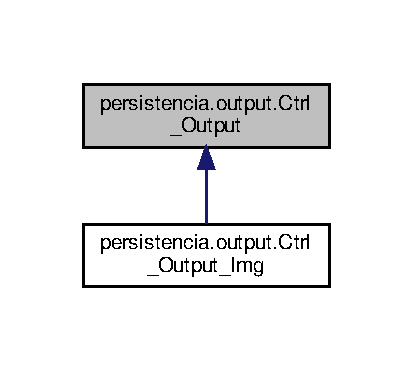
\includegraphics[width=198pt]{classpersistencia_1_1output_1_1Ctrl__Output__inherit__graph}
\end{center}
\end{figure}


Collaboration diagram for persistencia.\+output.\+Ctrl\+\_\+\+Output\+:\nopagebreak
\begin{figure}[H]
\begin{center}
\leavevmode
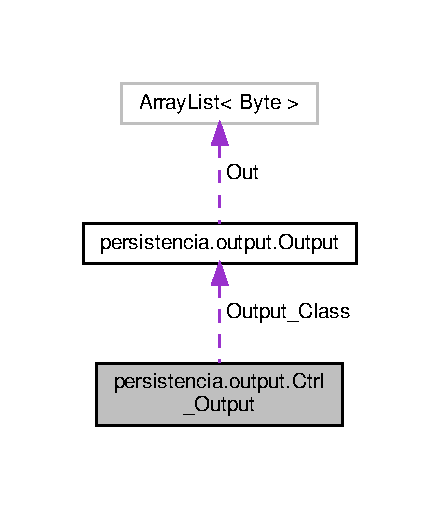
\includegraphics[width=211pt]{classpersistencia_1_1output_1_1Ctrl__Output__coll__graph}
\end{center}
\end{figure}
\subsection*{Public Member Functions}
\begin{DoxyCompactItemize}
\item 
\hyperlink{classpersistencia_1_1output_1_1Ctrl__Output_afeb28ec6172b522bf6bdaf16238d622b}{Ctrl\+\_\+\+Output} (String path, String method, boolean b)
\begin{DoxyCompactList}\small\item\em Constructor de la classe. \end{DoxyCompactList}\item 
void \hyperlink{classpersistencia_1_1output_1_1Ctrl__Output_a8c5aa5a6acb5259faeb1c05c71ddd21c}{add} (Byte b, Integer n\+\_\+bits)
\begin{DoxyCompactList}\small\item\em Afegeix un byte amb n\+\_\+bits valids. \end{DoxyCompactList}\item 
void \hyperlink{classpersistencia_1_1output_1_1Ctrl__Output_a0e3bedb0b88d0e60b228cc49143e6f0e}{add} (String s)
\begin{DoxyCompactList}\small\item\em Afegeix un String. \end{DoxyCompactList}\item 
void \hyperlink{classpersistencia_1_1output_1_1Ctrl__Output_a4070b40016edf1d959b3f7c60c90ef10}{add} (Character c)
\begin{DoxyCompactList}\small\item\em Afegeix un Character. \end{DoxyCompactList}\item 
void \hyperlink{classpersistencia_1_1output_1_1Ctrl__Output_aefe249b0ae9dbe578c44d96c6b56cf5d}{add} (Integer x)
\begin{DoxyCompactList}\small\item\em Afegeix un enter de 4 bytes. \end{DoxyCompactList}\item 
void \hyperlink{classpersistencia_1_1output_1_1Ctrl__Output_ac792cc55e30c9c769e10a20c2dd41bc8}{add} (Integer x, Integer mida)
\begin{DoxyCompactList}\small\item\em Afegeix un Integer d\textquotesingle{}una mida determinada. \end{DoxyCompactList}\item 
void \hyperlink{classpersistencia_1_1output_1_1Ctrl__Output_a5fb2f07198a77b4fac0f95ee48e3d0b9}{add} (Array\+List$<$ Byte $>$ arr)
\begin{DoxyCompactList}\small\item\em Afegeix una llista de Bytes. \end{DoxyCompactList}\item 
void \hyperlink{classpersistencia_1_1output_1_1Ctrl__Output_ad4738467c2312b0e079c14003e548dd6}{add2} (int x, int mida)
\begin{DoxyCompactList}\small\item\em Afegeix un enter amb mida. \end{DoxyCompactList}\item 
\mbox{\Hypertarget{classpersistencia_1_1output_1_1Ctrl__Output_a908955c29bfecc7ebac86613bc75e9ed}\label{classpersistencia_1_1output_1_1Ctrl__Output_a908955c29bfecc7ebac86613bc75e9ed}} 
void \hyperlink{classpersistencia_1_1output_1_1Ctrl__Output_a908955c29bfecc7ebac86613bc75e9ed}{print} ()
\begin{DoxyCompactList}\small\item\em Escriu el contingut de la classe en un nou arxiu. \end{DoxyCompactList}\item 
\mbox{\Hypertarget{classpersistencia_1_1output_1_1Ctrl__Output_a4536ad32e96d0270655a21c7c84f3bdd}\label{classpersistencia_1_1output_1_1Ctrl__Output_a4536ad32e96d0270655a21c7c84f3bdd}} 
void {\bfseries print\+String} ()
\item 
\hyperlink{classpersistencia_1_1output_1_1Output}{Output} \hyperlink{classpersistencia_1_1output_1_1Ctrl__Output_aa36fdf4d9efc14d95f5d0d77838c6280}{get\+Out} ()
\end{DoxyCompactItemize}
\subsection*{Package Attributes}
\begin{DoxyCompactItemize}
\item 
\hyperlink{classpersistencia_1_1output_1_1Output}{Output} \hyperlink{classpersistencia_1_1output_1_1Ctrl__Output_adbfbc3bef074ccf06131270fb9fafd8d}{Output\+\_\+\+Class}
\end{DoxyCompactItemize}


\subsection{Detailed Description}
Classe \hyperlink{classpersistencia_1_1output_1_1Ctrl__Output}{Ctrl\+\_\+\+Output}. 

\subsection{Constructor \& Destructor Documentation}
\mbox{\Hypertarget{classpersistencia_1_1output_1_1Ctrl__Output_afeb28ec6172b522bf6bdaf16238d622b}\label{classpersistencia_1_1output_1_1Ctrl__Output_afeb28ec6172b522bf6bdaf16238d622b}} 
\index{persistencia\+::output\+::\+Ctrl\+\_\+\+Output@{persistencia\+::output\+::\+Ctrl\+\_\+\+Output}!Ctrl\+\_\+\+Output@{Ctrl\+\_\+\+Output}}
\index{Ctrl\+\_\+\+Output@{Ctrl\+\_\+\+Output}!persistencia\+::output\+::\+Ctrl\+\_\+\+Output@{persistencia\+::output\+::\+Ctrl\+\_\+\+Output}}
\subsubsection{\texorpdfstring{Ctrl\+\_\+\+Output()}{Ctrl\_Output()}}
{\footnotesize\ttfamily persistencia.\+output.\+Ctrl\+\_\+\+Output.\+Ctrl\+\_\+\+Output (\begin{DoxyParamCaption}\item[{String}]{path,  }\item[{String}]{method,  }\item[{boolean}]{b }\end{DoxyParamCaption})\hspace{0.3cm}{\ttfamily [inline]}}



Constructor de la classe. 


\begin{DoxyParams}{Parameters}
{\em path} & Path de l\textquotesingle{}arxiu resultant de l\textquotesingle{}escritura \\
\hline
{\em method} & Indicara el valor de la metadata segons l\textquotesingle{}algoritme emprat \\
\hline
{\em b} & Indicació per a txt o ppm \\
\hline
\end{DoxyParams}


\subsection{Member Function Documentation}
\mbox{\Hypertarget{classpersistencia_1_1output_1_1Ctrl__Output_a8c5aa5a6acb5259faeb1c05c71ddd21c}\label{classpersistencia_1_1output_1_1Ctrl__Output_a8c5aa5a6acb5259faeb1c05c71ddd21c}} 
\index{persistencia\+::output\+::\+Ctrl\+\_\+\+Output@{persistencia\+::output\+::\+Ctrl\+\_\+\+Output}!add@{add}}
\index{add@{add}!persistencia\+::output\+::\+Ctrl\+\_\+\+Output@{persistencia\+::output\+::\+Ctrl\+\_\+\+Output}}
\subsubsection{\texorpdfstring{add()}{add()}\hspace{0.1cm}{\footnotesize\ttfamily [1/6]}}
{\footnotesize\ttfamily public void persistencia.\+output.\+Ctrl\+\_\+\+Output.\+add (\begin{DoxyParamCaption}\item[{Byte}]{b,  }\item[{Integer}]{n\+\_\+bits }\end{DoxyParamCaption})\hspace{0.3cm}{\ttfamily [inline]}}



Afegeix un byte amb n\+\_\+bits valids. 


\begin{DoxyParams}{Parameters}
{\em b} & Byte a afegir \\
\hline
{\em n\+\_\+bits} & Nombre de bits valids \\
\hline
\end{DoxyParams}
\mbox{\Hypertarget{classpersistencia_1_1output_1_1Ctrl__Output_a0e3bedb0b88d0e60b228cc49143e6f0e}\label{classpersistencia_1_1output_1_1Ctrl__Output_a0e3bedb0b88d0e60b228cc49143e6f0e}} 
\index{persistencia\+::output\+::\+Ctrl\+\_\+\+Output@{persistencia\+::output\+::\+Ctrl\+\_\+\+Output}!add@{add}}
\index{add@{add}!persistencia\+::output\+::\+Ctrl\+\_\+\+Output@{persistencia\+::output\+::\+Ctrl\+\_\+\+Output}}
\subsubsection{\texorpdfstring{add()}{add()}\hspace{0.1cm}{\footnotesize\ttfamily [2/6]}}
{\footnotesize\ttfamily public void persistencia.\+output.\+Ctrl\+\_\+\+Output.\+add (\begin{DoxyParamCaption}\item[{String}]{s }\end{DoxyParamCaption})\hspace{0.3cm}{\ttfamily [inline]}}



Afegeix un String. 


\begin{DoxyParams}{Parameters}
{\em s} & String a afegir \\
\hline
\end{DoxyParams}
\mbox{\Hypertarget{classpersistencia_1_1output_1_1Ctrl__Output_a4070b40016edf1d959b3f7c60c90ef10}\label{classpersistencia_1_1output_1_1Ctrl__Output_a4070b40016edf1d959b3f7c60c90ef10}} 
\index{persistencia\+::output\+::\+Ctrl\+\_\+\+Output@{persistencia\+::output\+::\+Ctrl\+\_\+\+Output}!add@{add}}
\index{add@{add}!persistencia\+::output\+::\+Ctrl\+\_\+\+Output@{persistencia\+::output\+::\+Ctrl\+\_\+\+Output}}
\subsubsection{\texorpdfstring{add()}{add()}\hspace{0.1cm}{\footnotesize\ttfamily [3/6]}}
{\footnotesize\ttfamily public void persistencia.\+output.\+Ctrl\+\_\+\+Output.\+add (\begin{DoxyParamCaption}\item[{Character}]{c }\end{DoxyParamCaption})\hspace{0.3cm}{\ttfamily [inline]}}



Afegeix un Character. 


\begin{DoxyParams}{Parameters}
{\em c} & Character a afegir \\
\hline
\end{DoxyParams}
\mbox{\Hypertarget{classpersistencia_1_1output_1_1Ctrl__Output_aefe249b0ae9dbe578c44d96c6b56cf5d}\label{classpersistencia_1_1output_1_1Ctrl__Output_aefe249b0ae9dbe578c44d96c6b56cf5d}} 
\index{persistencia\+::output\+::\+Ctrl\+\_\+\+Output@{persistencia\+::output\+::\+Ctrl\+\_\+\+Output}!add@{add}}
\index{add@{add}!persistencia\+::output\+::\+Ctrl\+\_\+\+Output@{persistencia\+::output\+::\+Ctrl\+\_\+\+Output}}
\subsubsection{\texorpdfstring{add()}{add()}\hspace{0.1cm}{\footnotesize\ttfamily [4/6]}}
{\footnotesize\ttfamily public void persistencia.\+output.\+Ctrl\+\_\+\+Output.\+add (\begin{DoxyParamCaption}\item[{Integer}]{x }\end{DoxyParamCaption})\hspace{0.3cm}{\ttfamily [inline]}}



Afegeix un enter de 4 bytes. 


\begin{DoxyParams}{Parameters}
{\em x} & Enter a afegir \\
\hline
\end{DoxyParams}
\mbox{\Hypertarget{classpersistencia_1_1output_1_1Ctrl__Output_ac792cc55e30c9c769e10a20c2dd41bc8}\label{classpersistencia_1_1output_1_1Ctrl__Output_ac792cc55e30c9c769e10a20c2dd41bc8}} 
\index{persistencia\+::output\+::\+Ctrl\+\_\+\+Output@{persistencia\+::output\+::\+Ctrl\+\_\+\+Output}!add@{add}}
\index{add@{add}!persistencia\+::output\+::\+Ctrl\+\_\+\+Output@{persistencia\+::output\+::\+Ctrl\+\_\+\+Output}}
\subsubsection{\texorpdfstring{add()}{add()}\hspace{0.1cm}{\footnotesize\ttfamily [5/6]}}
{\footnotesize\ttfamily public void persistencia.\+output.\+Ctrl\+\_\+\+Output.\+add (\begin{DoxyParamCaption}\item[{Integer}]{x,  }\item[{Integer}]{mida }\end{DoxyParamCaption})\hspace{0.3cm}{\ttfamily [inline]}}



Afegeix un Integer d\textquotesingle{}una mida determinada. 


\begin{DoxyParams}{Parameters}
{\em x} & Enter a afegir \\
\hline
{\em mida} & Mida del enter que volem afegir \\
\hline
\end{DoxyParams}
\mbox{\Hypertarget{classpersistencia_1_1output_1_1Ctrl__Output_a5fb2f07198a77b4fac0f95ee48e3d0b9}\label{classpersistencia_1_1output_1_1Ctrl__Output_a5fb2f07198a77b4fac0f95ee48e3d0b9}} 
\index{persistencia\+::output\+::\+Ctrl\+\_\+\+Output@{persistencia\+::output\+::\+Ctrl\+\_\+\+Output}!add@{add}}
\index{add@{add}!persistencia\+::output\+::\+Ctrl\+\_\+\+Output@{persistencia\+::output\+::\+Ctrl\+\_\+\+Output}}
\subsubsection{\texorpdfstring{add()}{add()}\hspace{0.1cm}{\footnotesize\ttfamily [6/6]}}
{\footnotesize\ttfamily public void persistencia.\+output.\+Ctrl\+\_\+\+Output.\+add (\begin{DoxyParamCaption}\item[{Array\+List$<$ Byte $>$}]{arr }\end{DoxyParamCaption})\hspace{0.3cm}{\ttfamily [inline]}}



Afegeix una llista de Bytes. 


\begin{DoxyParams}{Parameters}
{\em arr} & Llista a afegir \\
\hline
\end{DoxyParams}
\mbox{\Hypertarget{classpersistencia_1_1output_1_1Ctrl__Output_ad4738467c2312b0e079c14003e548dd6}\label{classpersistencia_1_1output_1_1Ctrl__Output_ad4738467c2312b0e079c14003e548dd6}} 
\index{persistencia\+::output\+::\+Ctrl\+\_\+\+Output@{persistencia\+::output\+::\+Ctrl\+\_\+\+Output}!add2@{add2}}
\index{add2@{add2}!persistencia\+::output\+::\+Ctrl\+\_\+\+Output@{persistencia\+::output\+::\+Ctrl\+\_\+\+Output}}
\subsubsection{\texorpdfstring{add2()}{add2()}}
{\footnotesize\ttfamily public void persistencia.\+output.\+Ctrl\+\_\+\+Output.\+add2 (\begin{DoxyParamCaption}\item[{int}]{x,  }\item[{int}]{mida }\end{DoxyParamCaption})\hspace{0.3cm}{\ttfamily [inline]}}



Afegeix un enter amb mida. 


\begin{DoxyParams}{Parameters}
{\em x} & Int a afegir. \\
\hline
{\em mida} & Mida de \char`\"{}x\char`\"{}. \\
\hline
\end{DoxyParams}
\mbox{\Hypertarget{classpersistencia_1_1output_1_1Ctrl__Output_aa36fdf4d9efc14d95f5d0d77838c6280}\label{classpersistencia_1_1output_1_1Ctrl__Output_aa36fdf4d9efc14d95f5d0d77838c6280}} 
\index{persistencia\+::output\+::\+Ctrl\+\_\+\+Output@{persistencia\+::output\+::\+Ctrl\+\_\+\+Output}!get\+Out@{get\+Out}}
\index{get\+Out@{get\+Out}!persistencia\+::output\+::\+Ctrl\+\_\+\+Output@{persistencia\+::output\+::\+Ctrl\+\_\+\+Output}}
\subsubsection{\texorpdfstring{get\+Out()}{getOut()}}
{\footnotesize\ttfamily public \hyperlink{classpersistencia_1_1output_1_1Output}{Output} persistencia.\+output.\+Ctrl\+\_\+\+Output.\+get\+Out (\begin{DoxyParamCaption}{ }\end{DoxyParamCaption})\hspace{0.3cm}{\ttfamily [inline]}}

\begin{DoxyReturn}{Returns}
Retorna l\textquotesingle{}atribut de tipus \hyperlink{classpersistencia_1_1output_1_1Output}{Output} de la classe 
\end{DoxyReturn}


\subsection{Member Data Documentation}
\mbox{\Hypertarget{classpersistencia_1_1output_1_1Ctrl__Output_adbfbc3bef074ccf06131270fb9fafd8d}\label{classpersistencia_1_1output_1_1Ctrl__Output_adbfbc3bef074ccf06131270fb9fafd8d}} 
\index{persistencia\+::output\+::\+Ctrl\+\_\+\+Output@{persistencia\+::output\+::\+Ctrl\+\_\+\+Output}!Output\+\_\+\+Class@{Output\+\_\+\+Class}}
\index{Output\+\_\+\+Class@{Output\+\_\+\+Class}!persistencia\+::output\+::\+Ctrl\+\_\+\+Output@{persistencia\+::output\+::\+Ctrl\+\_\+\+Output}}
\subsubsection{\texorpdfstring{Output\+\_\+\+Class}{Output\_Class}}
{\footnotesize\ttfamily \hyperlink{classpersistencia_1_1output_1_1Output}{Output} persistencia.\+output.\+Ctrl\+\_\+\+Output.\+Output\+\_\+\+Class\hspace{0.3cm}{\ttfamily [package]}}


\begin{DoxyParams}{Parameters}
{\em Output\+\_\+\+Class} & Classe \hyperlink{classpersistencia_1_1output_1_1Output}{Output} com atribut de la classe \\
\hline
\end{DoxyParams}


The documentation for this class was generated from the following file\+:\begin{DoxyCompactItemize}
\item 
src/persistencia/output/Ctrl\+\_\+\+Output.\+java\end{DoxyCompactItemize}

\hypertarget{classpersistencia_1_1output_1_1Ctrl__Output__Img}{}\section{persistencia.\+output.\+Ctrl\+\_\+\+Output\+\_\+\+Img Class Reference}
\label{classpersistencia_1_1output_1_1Ctrl__Output__Img}\index{persistencia.\+output.\+Ctrl\+\_\+\+Output\+\_\+\+Img@{persistencia.\+output.\+Ctrl\+\_\+\+Output\+\_\+\+Img}}


Inheritance diagram for persistencia.\+output.\+Ctrl\+\_\+\+Output\+\_\+\+Img\+:\nopagebreak
\begin{figure}[H]
\begin{center}
\leavevmode
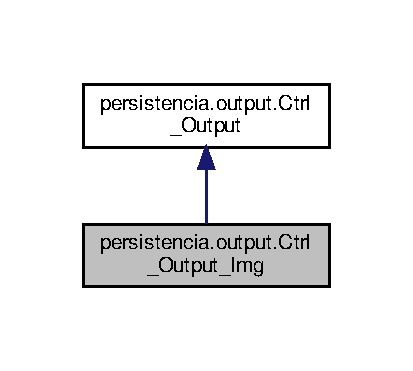
\includegraphics[width=198pt]{classpersistencia_1_1output_1_1Ctrl__Output__Img__inherit__graph}
\end{center}
\end{figure}


Collaboration diagram for persistencia.\+output.\+Ctrl\+\_\+\+Output\+\_\+\+Img\+:\nopagebreak
\begin{figure}[H]
\begin{center}
\leavevmode
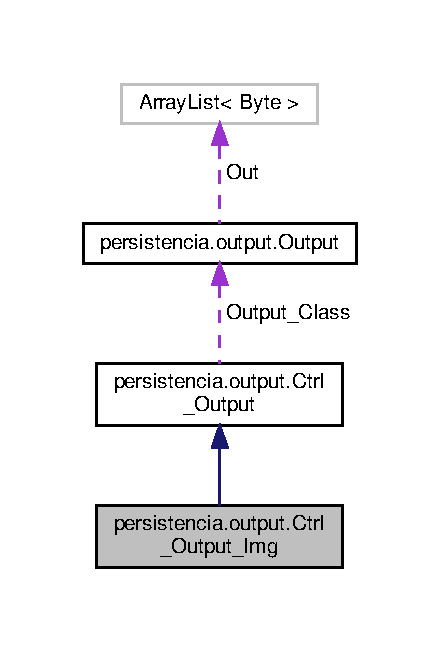
\includegraphics[width=211pt]{classpersistencia_1_1output_1_1Ctrl__Output__Img__coll__graph}
\end{center}
\end{figure}
\subsection*{Public Member Functions}
\begin{DoxyCompactItemize}
\item 
\mbox{\Hypertarget{classpersistencia_1_1output_1_1Ctrl__Output__Img_aa3f2948dd4645d8b121eedf30daa0c3f}\label{classpersistencia_1_1output_1_1Ctrl__Output__Img_aa3f2948dd4645d8b121eedf30daa0c3f}} 
{\bfseries Ctrl\+\_\+\+Output\+\_\+\+Img} (String path, int w, int h, int mv)
\item 
\mbox{\Hypertarget{classpersistencia_1_1output_1_1Ctrl__Output__Img_aaf087f80fc9410ca6edbe2cbc424b502}\label{classpersistencia_1_1output_1_1Ctrl__Output__Img_aaf087f80fc9410ca6edbe2cbc424b502}} 
int {\bfseries get\+Height} ()
\item 
\mbox{\Hypertarget{classpersistencia_1_1output_1_1Ctrl__Output__Img_a6efcf821f0a1097a7edd24c23e0da409}\label{classpersistencia_1_1output_1_1Ctrl__Output__Img_a6efcf821f0a1097a7edd24c23e0da409}} 
int {\bfseries get\+Width} ()
\item 
\mbox{\Hypertarget{classpersistencia_1_1output_1_1Ctrl__Output__Img_a305a977f4d4b999cf65e14e7106b6c5e}\label{classpersistencia_1_1output_1_1Ctrl__Output__Img_a305a977f4d4b999cf65e14e7106b6c5e}} 
void {\bfseries add} (double\mbox{[}$\,$\mbox{]}\mbox{[}$\,$\mbox{]}\mbox{[}$\,$\mbox{]}\mbox{[}$\,$\mbox{]} mat)
\item 
\mbox{\Hypertarget{classpersistencia_1_1output_1_1Ctrl__Output__Img_af8fd6acb8727f25014cc5ecca9a216cf}\label{classpersistencia_1_1output_1_1Ctrl__Output__Img_af8fd6acb8727f25014cc5ecca9a216cf}} 
boolean {\bfseries finished} ()
\end{DoxyCompactItemize}
\subsection*{Package Attributes}
\begin{DoxyCompactItemize}
\item 
\mbox{\Hypertarget{classpersistencia_1_1output_1_1Ctrl__Output__Img_ab9e685dae026afe43188c62d7c4fad53}\label{classpersistencia_1_1output_1_1Ctrl__Output__Img_ab9e685dae026afe43188c62d7c4fad53}} 
int {\bfseries max\+\_\+val}
\item 
\mbox{\Hypertarget{classpersistencia_1_1output_1_1Ctrl__Output__Img_a1d7bc52c64c79e8545ae6d1ae8b9ee2e}\label{classpersistencia_1_1output_1_1Ctrl__Output__Img_a1d7bc52c64c79e8545ae6d1ae8b9ee2e}} 
int {\bfseries height}
\item 
\mbox{\Hypertarget{classpersistencia_1_1output_1_1Ctrl__Output__Img_ae4a01ec459078cece4815d2fe7db8a64}\label{classpersistencia_1_1output_1_1Ctrl__Output__Img_ae4a01ec459078cece4815d2fe7db8a64}} 
int {\bfseries width}
\item 
\mbox{\Hypertarget{classpersistencia_1_1output_1_1Ctrl__Output__Img_ad40e63d16abd9058889249f5ad84f200}\label{classpersistencia_1_1output_1_1Ctrl__Output__Img_ad40e63d16abd9058889249f5ad84f200}} 
int {\bfseries bits\+\_\+per\+\_\+val}
\item 
\mbox{\Hypertarget{classpersistencia_1_1output_1_1Ctrl__Output__Img_a586ee8128a26b6786471e040a705bdbc}\label{classpersistencia_1_1output_1_1Ctrl__Output__Img_a586ee8128a26b6786471e040a705bdbc}} 
int {\bfseries rows}
\end{DoxyCompactItemize}


The documentation for this class was generated from the following file\+:\begin{DoxyCompactItemize}
\item 
src/persistencia/output/Ctrl\+\_\+\+Output\+\_\+\+Img.\+java\end{DoxyCompactItemize}

\hypertarget{classdomini_1_1utils_1_1Dict__Decode}{}\section{domini.\+utils.\+Dict\+\_\+\+Decode Class Reference}
\label{classdomini_1_1utils_1_1Dict__Decode}\index{domini.\+utils.\+Dict\+\_\+\+Decode@{domini.\+utils.\+Dict\+\_\+\+Decode}}


Diccionari (amb els mètodes corresponents) emprat per a la descompressió.  




Collaboration diagram for domini.\+utils.\+Dict\+\_\+\+Decode\+:\nopagebreak
\begin{figure}[H]
\begin{center}
\leavevmode
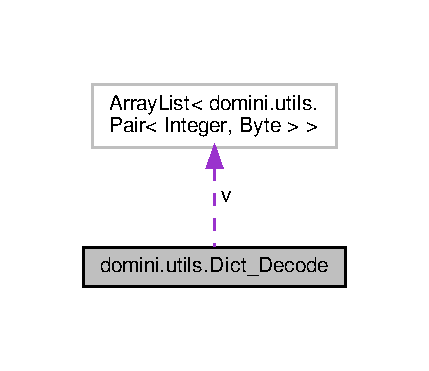
\includegraphics[width=206pt]{classdomini_1_1utils_1_1Dict__Decode__coll__graph}
\end{center}
\end{figure}
\subsection*{Public Member Functions}
\begin{DoxyCompactItemize}
\item 
\hyperlink{classdomini_1_1utils_1_1Dict__Decode_a8a0f9e67c530bafc031e72c218ce74f8}{Dict\+\_\+\+Decode} (Boolean inicialize\+Ascii, Integer \hyperlink{classdomini_1_1utils_1_1Dict__Decode_a6ef2d17f449cf7a658a4bf983e2fb474}{valor\+Neutre})
\begin{DoxyCompactList}\small\item\em Constructor de la classe. \end{DoxyCompactList}\item 
void \hyperlink{classdomini_1_1utils_1_1Dict__Decode_a635432505df1ceaa58a987bb80c6b0a3}{reset\+\_\+dictionary} (Boolean b)
\begin{DoxyCompactList}\small\item\em Reinicialitza el vector. \end{DoxyCompactList}\item 
Array\+List$<$ Byte $>$ \hyperlink{classdomini_1_1utils_1_1Dict__Decode_a0f6457460aefe9df50f0cad48f58feee}{get\+Word} (Integer i)
\begin{DoxyCompactList}\small\item\em Retorna la paraula que correspon a la seqüència encadenada a partir d\textquotesingle{}un enter. \end{DoxyCompactList}\item 
Integer \hyperlink{classdomini_1_1utils_1_1Dict__Decode_aac69020c3515649e8c2d70e2908e3f3e}{get\+Size} ()
\item 
void \hyperlink{classdomini_1_1utils_1_1Dict__Decode_a077011e4507db308d143ea9b7146abb9}{add} (Integer i, byte c)
\begin{DoxyCompactList}\small\item\em Afegeix un element al vector de la classe. \end{DoxyCompactList}\end{DoxyCompactItemize}
\subsection*{Package Attributes}
\begin{DoxyCompactItemize}
\item 
final Integer \hyperlink{classdomini_1_1utils_1_1Dict__Decode_a10fd6693de70b9091942496b35324c5a}{Limit} = Integer.\+M\+A\+X\+\_\+\+V\+A\+L\+UE
\item 
Array\+List$<$ \hyperlink{classdomini_1_1utils_1_1Pair}{Pair}$<$ Integer, Byte $>$ $>$ \hyperlink{classdomini_1_1utils_1_1Dict__Decode_a351bb8836b391e5e21ebc9cc1943a22d}{v}
\begin{DoxyCompactList}\small\item\em Cada element consta d\textquotesingle{}un byte i un index de la posició de la seqüència previa al byte actual. \end{DoxyCompactList}\item 
Integer \hyperlink{classdomini_1_1utils_1_1Dict__Decode_a6ef2d17f449cf7a658a4bf983e2fb474}{valor\+Neutre}
\end{DoxyCompactItemize}


\subsection{Detailed Description}
Diccionari (amb els mètodes corresponents) emprat per a la descompressió. 

Estructura de dades on cada posició indicarà una seqüencia de bytes b0,b1,...,bn-\/1,bn. El primer valor indica la posició del següent bytes de la subcadena b0,...,bn-\/1 mentre que el segon valor és bn. \begin{DoxyAuthor}{Author}
Miguel Paracuellos Ocaña 
\end{DoxyAuthor}


\subsection{Constructor \& Destructor Documentation}
\mbox{\Hypertarget{classdomini_1_1utils_1_1Dict__Decode_a8a0f9e67c530bafc031e72c218ce74f8}\label{classdomini_1_1utils_1_1Dict__Decode_a8a0f9e67c530bafc031e72c218ce74f8}} 
\index{domini\+::utils\+::\+Dict\+\_\+\+Decode@{domini\+::utils\+::\+Dict\+\_\+\+Decode}!Dict\+\_\+\+Decode@{Dict\+\_\+\+Decode}}
\index{Dict\+\_\+\+Decode@{Dict\+\_\+\+Decode}!domini\+::utils\+::\+Dict\+\_\+\+Decode@{domini\+::utils\+::\+Dict\+\_\+\+Decode}}
\subsubsection{\texorpdfstring{Dict\+\_\+\+Decode()}{Dict\_Decode()}}
{\footnotesize\ttfamily domini.\+utils.\+Dict\+\_\+\+Decode.\+Dict\+\_\+\+Decode (\begin{DoxyParamCaption}\item[{Boolean}]{inicialize\+Ascii,  }\item[{Integer}]{valor\+Neutre }\end{DoxyParamCaption})\hspace{0.3cm}{\ttfamily [inline]}}



Constructor de la classe. 

\begin{DoxyNote}{Note}
Inicialitzem el vector 
\end{DoxyNote}

\begin{DoxyParams}{Parameters}
{\em inicialize\+Ascii} & És true si inicialitzem només començar el diccionari amb la taula ascii. \\
\hline
{\em valor\+Neutre} & Valor \{0,1\} emprat a get\+Word \\
\hline
\end{DoxyParams}

\begin{DoxyCode}
32                                                                      \{
33         \hyperlink{classdomini_1_1utils_1_1Dict__Decode_a351bb8836b391e5e21ebc9cc1943a22d}{v} = \textcolor{keyword}{new} ArrayList<Pair<Integer,Byte> >();
34         \hyperlink{classdomini_1_1utils_1_1Dict__Decode_a635432505df1ceaa58a987bb80c6b0a3}{reset\_dictionary}(inicializeAscii);
35         this.\hyperlink{classdomini_1_1utils_1_1Dict__Decode_a6ef2d17f449cf7a658a4bf983e2fb474}{valorNeutre} = \hyperlink{classdomini_1_1utils_1_1Dict__Decode_a6ef2d17f449cf7a658a4bf983e2fb474}{valorNeutre};
36     \}
\end{DoxyCode}


\subsection{Member Function Documentation}
\mbox{\Hypertarget{classdomini_1_1utils_1_1Dict__Decode_a077011e4507db308d143ea9b7146abb9}\label{classdomini_1_1utils_1_1Dict__Decode_a077011e4507db308d143ea9b7146abb9}} 
\index{domini\+::utils\+::\+Dict\+\_\+\+Decode@{domini\+::utils\+::\+Dict\+\_\+\+Decode}!add@{add}}
\index{add@{add}!domini\+::utils\+::\+Dict\+\_\+\+Decode@{domini\+::utils\+::\+Dict\+\_\+\+Decode}}
\subsubsection{\texorpdfstring{add()}{add()}}
{\footnotesize\ttfamily public void domini.\+utils.\+Dict\+\_\+\+Decode.\+add (\begin{DoxyParamCaption}\item[{Integer}]{i,  }\item[{byte}]{c }\end{DoxyParamCaption})\hspace{0.3cm}{\ttfamily [inline]}}



Afegeix un element al vector de la classe. 


\begin{DoxyParams}{Parameters}
{\em i} & Enter que representa la cadena previa \\
\hline
{\em c} & Byte actual \\
\hline
\end{DoxyParams}

\begin{DoxyCode}
87                                        \{
88         \hyperlink{classdomini_1_1utils_1_1Dict__Decode_a351bb8836b391e5e21ebc9cc1943a22d}{v}.add( \textcolor{keyword}{new} Pair<Integer,Byte>(i,c) );
89     \}
\end{DoxyCode}
\mbox{\Hypertarget{classdomini_1_1utils_1_1Dict__Decode_aac69020c3515649e8c2d70e2908e3f3e}\label{classdomini_1_1utils_1_1Dict__Decode_aac69020c3515649e8c2d70e2908e3f3e}} 
\index{domini\+::utils\+::\+Dict\+\_\+\+Decode@{domini\+::utils\+::\+Dict\+\_\+\+Decode}!get\+Size@{get\+Size}}
\index{get\+Size@{get\+Size}!domini\+::utils\+::\+Dict\+\_\+\+Decode@{domini\+::utils\+::\+Dict\+\_\+\+Decode}}
\subsubsection{\texorpdfstring{get\+Size()}{getSize()}}
{\footnotesize\ttfamily public Integer domini.\+utils.\+Dict\+\_\+\+Decode.\+get\+Size (\begin{DoxyParamCaption}{ }\end{DoxyParamCaption})\hspace{0.3cm}{\ttfamily [inline]}}

\begin{DoxyReturn}{Returns}
Size del vector 
\end{DoxyReturn}

\begin{DoxyCode}
77                              \{
78         \textcolor{keywordflow}{return} \hyperlink{classdomini_1_1utils_1_1Dict__Decode_a351bb8836b391e5e21ebc9cc1943a22d}{v}.size();
79     \}
\end{DoxyCode}
\mbox{\Hypertarget{classdomini_1_1utils_1_1Dict__Decode_a0f6457460aefe9df50f0cad48f58feee}\label{classdomini_1_1utils_1_1Dict__Decode_a0f6457460aefe9df50f0cad48f58feee}} 
\index{domini\+::utils\+::\+Dict\+\_\+\+Decode@{domini\+::utils\+::\+Dict\+\_\+\+Decode}!get\+Word@{get\+Word}}
\index{get\+Word@{get\+Word}!domini\+::utils\+::\+Dict\+\_\+\+Decode@{domini\+::utils\+::\+Dict\+\_\+\+Decode}}
\subsubsection{\texorpdfstring{get\+Word()}{getWord()}}
{\footnotesize\ttfamily public String domini.\+utils.\+Dict\+\_\+\+Decode.\+get\+Word (\begin{DoxyParamCaption}\item[{Integer}]{i }\end{DoxyParamCaption})\hspace{0.3cm}{\ttfamily [inline]}}



Retorna la paraula que correspon a la seqüència encadenada a partir d\textquotesingle{}un enter. 


\begin{DoxyParams}{Parameters}
{\em i} & Enter que representa una seqüència de caràcters \\
\hline
\end{DoxyParams}
\begin{DoxyReturn}{Returns}
Retorna la paraula corresponent a l\textquotesingle{}enter 
\end{DoxyReturn}

\begin{DoxyCode}
60                                               \{
61         ArrayList<Byte> result = \textcolor{keyword}{new} ArrayList<>();
62         result.clear();
63         \textcolor{comment}{//result.ensureCapacity(Limit);}
64         Integer diff = this.\hyperlink{classdomini_1_1utils_1_1Dict__Decode_a6ef2d17f449cf7a658a4bf983e2fb474}{valorNeutre} +1;
65         \textcolor{keywordflow}{while} (i != this.\hyperlink{classdomini_1_1utils_1_1Dict__Decode_a6ef2d17f449cf7a658a4bf983e2fb474}{valorNeutre}) \{
66             result.add(0, \hyperlink{classdomini_1_1utils_1_1Dict__Decode_a351bb8836b391e5e21ebc9cc1943a22d}{v}.get(i-diff).getRight());
67             i = \hyperlink{classdomini_1_1utils_1_1Dict__Decode_a351bb8836b391e5e21ebc9cc1943a22d}{v}.get(i-diff).getLeft();
68         \}
69 
70         \textcolor{keywordflow}{return} result;
71     \}
\end{DoxyCode}
\mbox{\Hypertarget{classdomini_1_1utils_1_1Dict__Decode_a635432505df1ceaa58a987bb80c6b0a3}\label{classdomini_1_1utils_1_1Dict__Decode_a635432505df1ceaa58a987bb80c6b0a3}} 
\index{domini\+::utils\+::\+Dict\+\_\+\+Decode@{domini\+::utils\+::\+Dict\+\_\+\+Decode}!reset\+\_\+dictionary@{reset\+\_\+dictionary}}
\index{reset\+\_\+dictionary@{reset\+\_\+dictionary}!domini\+::utils\+::\+Dict\+\_\+\+Decode@{domini\+::utils\+::\+Dict\+\_\+\+Decode}}
\subsubsection{\texorpdfstring{reset\+\_\+dictionary()}{reset\_dictionary()}}
{\footnotesize\ttfamily void domini.\+utils.\+Dict\+\_\+\+Decode.\+reset\+\_\+dictionary (\begin{DoxyParamCaption}\item[{Boolean}]{b }\end{DoxyParamCaption})\hspace{0.3cm}{\ttfamily [inline]}}



Reinicialitza el vector. 

\begin{DoxyNote}{Note}
Es crida quan sigui ple o si es instanciat a la construcció. 
\end{DoxyNote}

\begin{DoxyParams}{Parameters}
{\em b} & Es true si volem inicialitzar el diccionari amb la taula A\+S\+C\+II \\
\hline
\end{DoxyParams}

\begin{DoxyCode}
43                                             \{
44         \hyperlink{classdomini_1_1utils_1_1Dict__Decode_a351bb8836b391e5e21ebc9cc1943a22d}{v}.clear();
45         \textcolor{comment}{//v.ensureCapacity(Limit);}
46         \textcolor{keywordflow}{if}(!b)return ;
47         \textcolor{keywordflow}{for} (\textcolor{keywordtype}{int} i = 0; i < 256; ++i) \{
48             \hyperlink{classdomini_1_1utils_1_1Dict__Decode_a351bb8836b391e5e21ebc9cc1943a22d}{v}.add( \textcolor{keyword}{new} Pair<Integer,Byte>(-1, (byte)i) );
49         \}
50     \}
\end{DoxyCode}


\subsection{Member Data Documentation}
\mbox{\Hypertarget{classdomini_1_1utils_1_1Dict__Decode_a10fd6693de70b9091942496b35324c5a}\label{classdomini_1_1utils_1_1Dict__Decode_a10fd6693de70b9091942496b35324c5a}} 
\index{domini\+::utils\+::\+Dict\+\_\+\+Decode@{domini\+::utils\+::\+Dict\+\_\+\+Decode}!Limit@{Limit}}
\index{Limit@{Limit}!domini\+::utils\+::\+Dict\+\_\+\+Decode@{domini\+::utils\+::\+Dict\+\_\+\+Decode}}
\subsubsection{\texorpdfstring{Limit}{Limit}}
{\footnotesize\ttfamily final Integer domini.\+utils.\+Dict\+\_\+\+Decode.\+Limit = Integer.\+M\+A\+X\+\_\+\+V\+A\+L\+UE\hspace{0.3cm}{\ttfamily [package]}}


\begin{DoxyParams}{Parameters}
{\em Limit} & Màxim nombre d\textquotesingle{}entrades que pot tenir el diccionari \\
\hline
\end{DoxyParams}
\mbox{\Hypertarget{classdomini_1_1utils_1_1Dict__Decode_a351bb8836b391e5e21ebc9cc1943a22d}\label{classdomini_1_1utils_1_1Dict__Decode_a351bb8836b391e5e21ebc9cc1943a22d}} 
\index{domini\+::utils\+::\+Dict\+\_\+\+Decode@{domini\+::utils\+::\+Dict\+\_\+\+Decode}!v@{v}}
\index{v@{v}!domini\+::utils\+::\+Dict\+\_\+\+Decode@{domini\+::utils\+::\+Dict\+\_\+\+Decode}}
\subsubsection{\texorpdfstring{v}{v}}
{\footnotesize\ttfamily Array\+List$<$\hyperlink{classdomini_1_1utils_1_1Pair}{Pair}$<$Integer,Byte$>$ $>$ domini.\+utils.\+Dict\+\_\+\+Decode.\+v\hspace{0.3cm}{\ttfamily [package]}}



Cada element consta d\textquotesingle{}un byte i un index de la posició de la seqüència previa al byte actual. 


\begin{DoxyParams}{Parameters}
{\em v} & Diccionari de la classe \\
\hline
\end{DoxyParams}
\mbox{\Hypertarget{classdomini_1_1utils_1_1Dict__Decode_a6ef2d17f449cf7a658a4bf983e2fb474}\label{classdomini_1_1utils_1_1Dict__Decode_a6ef2d17f449cf7a658a4bf983e2fb474}} 
\index{domini\+::utils\+::\+Dict\+\_\+\+Decode@{domini\+::utils\+::\+Dict\+\_\+\+Decode}!valor\+Neutre@{valor\+Neutre}}
\index{valor\+Neutre@{valor\+Neutre}!domini\+::utils\+::\+Dict\+\_\+\+Decode@{domini\+::utils\+::\+Dict\+\_\+\+Decode}}
\subsubsection{\texorpdfstring{valor\+Neutre}{valorNeutre}}
{\footnotesize\ttfamily Integer domini.\+utils.\+Dict\+\_\+\+Decode.\+valor\+Neutre\hspace{0.3cm}{\ttfamily [package]}}



The documentation for this class was generated from the following file\+:\begin{DoxyCompactItemize}
\item 
src/domini/utils/\hyperlink{Dict__Decode_8java}{Dict\+\_\+\+Decode.\+java}\end{DoxyCompactItemize}

\hypertarget{classdomini_1_1utils_1_1Dict__Encode}{}\section{domini.\+utils.\+Dict\+\_\+\+Encode Class Reference}
\label{classdomini_1_1utils_1_1Dict__Encode}\index{domini.\+utils.\+Dict\+\_\+\+Encode@{domini.\+utils.\+Dict\+\_\+\+Encode}}


Diccionari (amb els mètodes corresponents) emprat per a la compressió amb L\+ZW.  


\subsection*{Public Member Functions}
\begin{DoxyCompactItemize}
\item 
\hyperlink{classdomini_1_1utils_1_1Dict__Encode_aa16372a031311494fdcae13d1a9b48c3}{Dict\+\_\+\+Encode} ()
\begin{DoxyCompactList}\small\item\em Constructor de la classe. \end{DoxyCompactList}\item 
void \hyperlink{classdomini_1_1utils_1_1Dict__Encode_a6c3016286b3bb242d12799f8e7ebb585}{reset\+\_\+dictionary} ()
\begin{DoxyCompactList}\small\item\em Reinicilització del diccionari de la classe. \end{DoxyCompactList}\item 
Integer \hyperlink{classdomini_1_1utils_1_1Dict__Encode_a12e23ecdd9b0078cb6e56c01126248b9}{Ascii\+\_\+value} (byte c)
\begin{DoxyCompactList}\small\item\em Retorna el valor númeric d\textquotesingle{}un caràcter A\+S\+C\+II. \end{DoxyCompactList}\item 
Integer \hyperlink{classdomini_1_1utils_1_1Dict__Encode_a1bafdca1835da3fa93b900ff0aa720e0}{search\+\_\+and\+\_\+insert\+\_\+\+B\+ST} (Integer i, byte c)
\begin{DoxyCompactList}\small\item\em Cada cop que es crida es mira si ja tenim la combinació enter-\/char al diccionari. \end{DoxyCompactList}\item 
Integer \hyperlink{classdomini_1_1utils_1_1Dict__Encode_a21a05b62b848a7ab9fbdf49a3a6e7edf}{get\+Limit} ()
\end{DoxyCompactItemize}
\subsection*{Static Public Attributes}
\begin{DoxyCompactItemize}
\item 
static final Integer \hyperlink{classdomini_1_1utils_1_1Dict__Encode_a48fe9a878056a119ad36a0aad2727a13}{Limit} = Integer.\+M\+A\+X\+\_\+\+V\+A\+L\+UE
\end{DoxyCompactItemize}


\subsection{Detailed Description}
Diccionari (amb els mètodes corresponents) emprat per a la compressió amb L\+ZW. 

\begin{DoxyAuthor}{Author}
Miguel Paracuellos Ocaña 
\end{DoxyAuthor}


\subsection{Constructor \& Destructor Documentation}
\mbox{\Hypertarget{classdomini_1_1utils_1_1Dict__Encode_aa16372a031311494fdcae13d1a9b48c3}\label{classdomini_1_1utils_1_1Dict__Encode_aa16372a031311494fdcae13d1a9b48c3}} 
\index{domini\+::utils\+::\+Dict\+\_\+\+Encode@{domini\+::utils\+::\+Dict\+\_\+\+Encode}!Dict\+\_\+\+Encode@{Dict\+\_\+\+Encode}}
\index{Dict\+\_\+\+Encode@{Dict\+\_\+\+Encode}!domini\+::utils\+::\+Dict\+\_\+\+Encode@{domini\+::utils\+::\+Dict\+\_\+\+Encode}}
\subsubsection{\texorpdfstring{Dict\+\_\+\+Encode()}{Dict\_Encode()}}
{\footnotesize\ttfamily domini.\+utils.\+Dict\+\_\+\+Encode.\+Dict\+\_\+\+Encode (\begin{DoxyParamCaption}{ }\end{DoxyParamCaption})\hspace{0.3cm}{\ttfamily [inline]}}



Constructor de la classe. 

\begin{DoxyNote}{Note}
Inicialitzem el diccionari 
\end{DoxyNote}


\subsection{Member Function Documentation}
\mbox{\Hypertarget{classdomini_1_1utils_1_1Dict__Encode_a12e23ecdd9b0078cb6e56c01126248b9}\label{classdomini_1_1utils_1_1Dict__Encode_a12e23ecdd9b0078cb6e56c01126248b9}} 
\index{domini\+::utils\+::\+Dict\+\_\+\+Encode@{domini\+::utils\+::\+Dict\+\_\+\+Encode}!Ascii\+\_\+value@{Ascii\+\_\+value}}
\index{Ascii\+\_\+value@{Ascii\+\_\+value}!domini\+::utils\+::\+Dict\+\_\+\+Encode@{domini\+::utils\+::\+Dict\+\_\+\+Encode}}
\subsubsection{\texorpdfstring{Ascii\+\_\+value()}{Ascii\_value()}}
{\footnotesize\ttfamily public Integer domini.\+utils.\+Dict\+\_\+\+Encode.\+Ascii\+\_\+value (\begin{DoxyParamCaption}\item[{byte}]{c }\end{DoxyParamCaption})\hspace{0.3cm}{\ttfamily [inline]}}



Retorna el valor númeric d\textquotesingle{}un caràcter A\+S\+C\+II. 


\begin{DoxyParams}{Parameters}
{\em c} & Caràcter que volem passar a valor numeric \\
\hline
\end{DoxyParams}
\begin{DoxyReturn}{Returns}
Valor numeric del caràcter 
\end{DoxyReturn}
\mbox{\Hypertarget{classdomini_1_1utils_1_1Dict__Encode_a21a05b62b848a7ab9fbdf49a3a6e7edf}\label{classdomini_1_1utils_1_1Dict__Encode_a21a05b62b848a7ab9fbdf49a3a6e7edf}} 
\index{domini\+::utils\+::\+Dict\+\_\+\+Encode@{domini\+::utils\+::\+Dict\+\_\+\+Encode}!get\+Limit@{get\+Limit}}
\index{get\+Limit@{get\+Limit}!domini\+::utils\+::\+Dict\+\_\+\+Encode@{domini\+::utils\+::\+Dict\+\_\+\+Encode}}
\subsubsection{\texorpdfstring{get\+Limit()}{getLimit()}}
{\footnotesize\ttfamily public Integer domini.\+utils.\+Dict\+\_\+\+Encode.\+get\+Limit (\begin{DoxyParamCaption}{ }\end{DoxyParamCaption})\hspace{0.3cm}{\ttfamily [inline]}}

\begin{DoxyReturn}{Returns}
Retorna el limit d\textquotesingle{}entrades que pot tenir el diccionari 
\end{DoxyReturn}
\mbox{\Hypertarget{classdomini_1_1utils_1_1Dict__Encode_a6c3016286b3bb242d12799f8e7ebb585}\label{classdomini_1_1utils_1_1Dict__Encode_a6c3016286b3bb242d12799f8e7ebb585}} 
\index{domini\+::utils\+::\+Dict\+\_\+\+Encode@{domini\+::utils\+::\+Dict\+\_\+\+Encode}!reset\+\_\+dictionary@{reset\+\_\+dictionary}}
\index{reset\+\_\+dictionary@{reset\+\_\+dictionary}!domini\+::utils\+::\+Dict\+\_\+\+Encode@{domini\+::utils\+::\+Dict\+\_\+\+Encode}}
\subsubsection{\texorpdfstring{reset\+\_\+dictionary()}{reset\_dictionary()}}
{\footnotesize\ttfamily public void domini.\+utils.\+Dict\+\_\+\+Encode.\+reset\+\_\+dictionary (\begin{DoxyParamCaption}{ }\end{DoxyParamCaption})\hspace{0.3cm}{\ttfamily [inline]}}



Reinicilització del diccionari de la classe. 

\begin{DoxyNote}{Note}
Només quan el creem o quan estigui ple 
\end{DoxyNote}
\mbox{\Hypertarget{classdomini_1_1utils_1_1Dict__Encode_a1bafdca1835da3fa93b900ff0aa720e0}\label{classdomini_1_1utils_1_1Dict__Encode_a1bafdca1835da3fa93b900ff0aa720e0}} 
\index{domini\+::utils\+::\+Dict\+\_\+\+Encode@{domini\+::utils\+::\+Dict\+\_\+\+Encode}!search\+\_\+and\+\_\+insert\+\_\+\+B\+ST@{search\+\_\+and\+\_\+insert\+\_\+\+B\+ST}}
\index{search\+\_\+and\+\_\+insert\+\_\+\+B\+ST@{search\+\_\+and\+\_\+insert\+\_\+\+B\+ST}!domini\+::utils\+::\+Dict\+\_\+\+Encode@{domini\+::utils\+::\+Dict\+\_\+\+Encode}}
\subsubsection{\texorpdfstring{search\+\_\+and\+\_\+insert\+\_\+\+B\+S\+T()}{search\_and\_insert\_BST()}}
{\footnotesize\ttfamily public Integer domini.\+utils.\+Dict\+\_\+\+Encode.\+search\+\_\+and\+\_\+insert\+\_\+\+B\+ST (\begin{DoxyParamCaption}\item[{Integer}]{i,  }\item[{byte}]{c }\end{DoxyParamCaption})\hspace{0.3cm}{\ttfamily [inline]}}



Cada cop que es crida es mira si ja tenim la combinació enter-\/char al diccionari. 


\begin{DoxyParams}{Parameters}
{\em i} & Enter que representa una cadena de caràcters \\
\hline
{\em c} & Caràcter actual \\
\hline
\end{DoxyParams}
\begin{DoxyReturn}{Returns}
Retorna l\textquotesingle{}enter que farà referència a la nova cadena de caràcters 
\end{DoxyReturn}


\subsection{Member Data Documentation}
\mbox{\Hypertarget{classdomini_1_1utils_1_1Dict__Encode_a48fe9a878056a119ad36a0aad2727a13}\label{classdomini_1_1utils_1_1Dict__Encode_a48fe9a878056a119ad36a0aad2727a13}} 
\index{domini\+::utils\+::\+Dict\+\_\+\+Encode@{domini\+::utils\+::\+Dict\+\_\+\+Encode}!Limit@{Limit}}
\index{Limit@{Limit}!domini\+::utils\+::\+Dict\+\_\+\+Encode@{domini\+::utils\+::\+Dict\+\_\+\+Encode}}
\subsubsection{\texorpdfstring{Limit}{Limit}}
{\footnotesize\ttfamily final Integer domini.\+utils.\+Dict\+\_\+\+Encode.\+Limit = Integer.\+M\+A\+X\+\_\+\+V\+A\+L\+UE\hspace{0.3cm}{\ttfamily [static]}}


\begin{DoxyParams}{Parameters}
{\em Limit} & Nombre màxim d\textquotesingle{}entrades que pot tenir el diccionari \\
\hline
\end{DoxyParams}


The documentation for this class was generated from the following file\+:\begin{DoxyCompactItemize}
\item 
src/domini/utils/Dict\+\_\+\+Encode.\+java\end{DoxyCompactItemize}

\hypertarget{classdomini_1_1utils_1_1Driver____ArrayCircular}{}\section{domini.\+utils.\+Driver\+\_\+\+\_\+\+Array\+Circular Class Reference}
\label{classdomini_1_1utils_1_1Driver____ArrayCircular}\index{domini.\+utils.\+Driver\+\_\+\+\_\+\+Array\+Circular@{domini.\+utils.\+Driver\+\_\+\+\_\+\+Array\+Circular}}


Driver de \hyperlink{classdomini_1_1utils_1_1ArrayCircular}{Array\+Circular}.  


\subsection*{Static Public Member Functions}
\begin{DoxyCompactItemize}
\item 
static void \hyperlink{classdomini_1_1utils_1_1Driver____ArrayCircular_adf8b1dedd521248da8a5f1425dd27af8}{main} (String\mbox{[}$\,$\mbox{]} args)
\end{DoxyCompactItemize}
\subsection*{Static Private Member Functions}
\begin{DoxyCompactItemize}
\item 
static void \hyperlink{classdomini_1_1utils_1_1Driver____ArrayCircular_afac5a37f91b2914e692993e71c2d393c}{show\+Options} ()
\begin{DoxyCompactList}\small\item\em Mostra les accions a realitzar durant l\textquotesingle{}execució \end{DoxyCompactList}\item 
static void \hyperlink{classdomini_1_1utils_1_1Driver____ArrayCircular_a0f5f42c5ace9176cfcae4dfe9717f380}{comprovar\+Excepcions} (\hyperlink{classdomini_1_1utils_1_1ArrayCircular}{Array\+Circular} arraycircular, String linea)
\begin{DoxyCompactList}\small\item\em Comprovarà les possibles excepcions que puguin apareixer a la classe. \end{DoxyCompactList}\end{DoxyCompactItemize}


\subsection{Detailed Description}
Driver de \hyperlink{classdomini_1_1utils_1_1ArrayCircular}{Array\+Circular}. 

\begin{DoxyAuthor}{Author}
Joan Bellavista Bartroli 
\end{DoxyAuthor}


\subsection{Member Function Documentation}
\mbox{\Hypertarget{classdomini_1_1utils_1_1Driver____ArrayCircular_a0f5f42c5ace9176cfcae4dfe9717f380}\label{classdomini_1_1utils_1_1Driver____ArrayCircular_a0f5f42c5ace9176cfcae4dfe9717f380}} 
\index{domini\+::utils\+::\+Driver\+\_\+\+\_\+\+Array\+Circular@{domini\+::utils\+::\+Driver\+\_\+\+\_\+\+Array\+Circular}!comprovar\+Excepcions@{comprovar\+Excepcions}}
\index{comprovar\+Excepcions@{comprovar\+Excepcions}!domini\+::utils\+::\+Driver\+\_\+\+\_\+\+Array\+Circular@{domini\+::utils\+::\+Driver\+\_\+\+\_\+\+Array\+Circular}}
\subsubsection{\texorpdfstring{comprovar\+Excepcions()}{comprovarExcepcions()}}
{\footnotesize\ttfamily private static void domini.\+utils.\+Driver\+\_\+\+\_\+\+Array\+Circular.\+comprovar\+Excepcions (\begin{DoxyParamCaption}\item[{\hyperlink{classdomini_1_1utils_1_1ArrayCircular}{Array\+Circular}}]{arraycircular,  }\item[{String}]{linea }\end{DoxyParamCaption})\hspace{0.3cm}{\ttfamily [inline]}, {\ttfamily [static]}, {\ttfamily [private]}}



Comprovarà les possibles excepcions que puguin apareixer a la classe. 


\begin{DoxyParams}{Parameters}
{\em arraycircular} & Instància \hyperlink{classdomini_1_1utils_1_1ArrayCircular}{Array\+Circular} \\
\hline
{\em linea} & Número de operació realitzada \\
\hline
\end{DoxyParams}

\begin{DoxyCode}
49                                                                                       \{
50         \textcolor{keywordtype}{int} op = Integer.parseInt(linea);
51         \textcolor{keywordflow}{if}(arraycircular == null && op > 1) \{
52             \textcolor{keywordflow}{throw} \textcolor{keyword}{new} IllegalArgumentException(\textcolor{stringliteral}{"Debes llamar al constructor antes"});
53         \}
54     \}
\end{DoxyCode}
\mbox{\Hypertarget{classdomini_1_1utils_1_1Driver____ArrayCircular_adf8b1dedd521248da8a5f1425dd27af8}\label{classdomini_1_1utils_1_1Driver____ArrayCircular_adf8b1dedd521248da8a5f1425dd27af8}} 
\index{domini\+::utils\+::\+Driver\+\_\+\+\_\+\+Array\+Circular@{domini\+::utils\+::\+Driver\+\_\+\+\_\+\+Array\+Circular}!main@{main}}
\index{main@{main}!domini\+::utils\+::\+Driver\+\_\+\+\_\+\+Array\+Circular@{domini\+::utils\+::\+Driver\+\_\+\+\_\+\+Array\+Circular}}
\subsubsection{\texorpdfstring{main()}{main()}}
{\footnotesize\ttfamily static void domini.\+utils.\+Driver\+\_\+\+\_\+\+Array\+Circular.\+main (\begin{DoxyParamCaption}\item[{String \mbox{[}$\,$\mbox{]}}]{args }\end{DoxyParamCaption})\hspace{0.3cm}{\ttfamily [inline]}, {\ttfamily [static]}}


\begin{DoxyCode}
56                                            \{
57     \textcolor{keywordflow}{try} \{
58         ArrayCircular arraycircular = null;
59         \hyperlink{classdomini_1_1utils_1_1Driver____ArrayCircular_afac5a37f91b2914e692993e71c2d393c}{showOptions}();
60         BufferedReader reader = \textcolor{keyword}{new} BufferedReader(\textcolor{keyword}{new} InputStreamReader(System.in));
61         String linea = \textcolor{stringliteral}{""};
62         \textcolor{keywordflow}{while}(linea != null)\{
63             System.out.println(\textcolor{stringliteral}{"Selecciona una opción:"});
64             linea = reader.readLine().trim();
65             System.out.println(\textcolor{stringliteral}{"Opción: "} + linea + \textcolor{stringliteral}{" seleccionada"});
66             \hyperlink{classdomini_1_1utils_1_1Driver____ArrayCircular_a0f5f42c5ace9176cfcae4dfe9717f380}{comprovarExcepcions}(arraycircular, linea);
67             \textcolor{keywordflow}{switch}(linea)\{
68                 \textcolor{keywordflow}{case} \textcolor{stringliteral}{"1"}:
69                     System.out.println(\textcolor{stringliteral}{"Pon un entero que representará el tamaño"});
70                     String aux = reader.readLine().trim();
71                     \textcolor{keywordtype}{int} mida = Integer.parseInt(aux);
72                     arraycircular = \textcolor{keyword}{new} ArrayCircular(mida);
73                 \textcolor{keywordflow}{break};
74                 \textcolor{keywordflow}{case} \textcolor{stringliteral}{"2"}:
75                     System.out.println(\textcolor{stringliteral}{"Pon un Byte para añadir a la ArrayCircular"});
76                     aux = reader.readLine().trim();
77                     byte value = Byte.parseByte(aux);
78                     arraycircular.setValue(value);
79                 \textcolor{keywordflow}{break};
80                 \textcolor{keywordflow}{case} \textcolor{stringliteral}{"3"}:
81                     System.out.println(\textcolor{stringliteral}{"Pon un entero para conseguir el valor en esa posición"});
82                     aux = reader.readLine().trim();
83                     \textcolor{keywordtype}{int} index = Integer.parseInt(aux);
84                     System.out.println(arraycircular.getValue(index));;
85                 \textcolor{keywordflow}{break};
86                 \textcolor{keywordflow}{case} \textcolor{stringliteral}{"4"}:
87                     System.out.println(\textcolor{stringliteral}{"Pon un entero"});
88                     aux = reader.readLine().trim();
89                     \textcolor{keywordtype}{int} despl = Integer.parseInt(aux);
90                     System.out.println(arraycircular.getValueAmbDespl(despl));;
91                 \textcolor{keywordflow}{break};
92                 \textcolor{keywordflow}{case} \textcolor{stringliteral}{"5"}:
93                     System.out.println(arraycircular.getStart());;
94                 \textcolor{keywordflow}{break};
95                 \textcolor{keywordflow}{case} \textcolor{stringliteral}{"6"}:
96                     System.out.println(arraycircular.getEnd());;
97                 \textcolor{keywordflow}{break};
98                 \textcolor{keywordflow}{case} \textcolor{stringliteral}{"7"}:
99                     System.out.println(\textcolor{stringliteral}{"Pon un Byte para saber si está en la Array"});
100                     aux = reader.readLine().trim();
101                     value = Byte.parseByte(aux);
102                     System.out.println(arraycircular.isIn(value));;
103                 \textcolor{keywordflow}{break};
104                 \textcolor{keywordflow}{case} \textcolor{stringliteral}{"8"}:
105                     System.out.println(arraycircular.getAfegits());
106                 \textcolor{keywordflow}{break};
107                 \textcolor{keywordflow}{case} \textcolor{stringliteral}{"0"}:
108                     \textcolor{keywordflow}{return};
109                 \textcolor{keywordflow}{default}:
110                     System.out.println(\textcolor{stringliteral}{"La opción no es válida"});
111                 \textcolor{keywordflow}{break};
112             \}
113         \}
114     \}\textcolor{keywordflow}{catch} (Exception e) \{
115         e.printStackTrace();
116     \}
117     \}
\end{DoxyCode}
\mbox{\Hypertarget{classdomini_1_1utils_1_1Driver____ArrayCircular_afac5a37f91b2914e692993e71c2d393c}\label{classdomini_1_1utils_1_1Driver____ArrayCircular_afac5a37f91b2914e692993e71c2d393c}} 
\index{domini\+::utils\+::\+Driver\+\_\+\+\_\+\+Array\+Circular@{domini\+::utils\+::\+Driver\+\_\+\+\_\+\+Array\+Circular}!show\+Options@{show\+Options}}
\index{show\+Options@{show\+Options}!domini\+::utils\+::\+Driver\+\_\+\+\_\+\+Array\+Circular@{domini\+::utils\+::\+Driver\+\_\+\+\_\+\+Array\+Circular}}
\subsubsection{\texorpdfstring{show\+Options()}{showOptions()}}
{\footnotesize\ttfamily private static void domini.\+utils.\+Driver\+\_\+\+\_\+\+Array\+Circular.\+show\+Options (\begin{DoxyParamCaption}{ }\end{DoxyParamCaption})\hspace{0.3cm}{\ttfamily [inline]}, {\ttfamily [static]}, {\ttfamily [private]}}



Mostra les accions a realitzar durant l\textquotesingle{}execució 


\begin{DoxyCode}
17                                      \{
18         System.out.println(\textcolor{stringliteral}{"Driver de ArrayCircular"});
19         System.out.println(\textcolor{stringliteral}{"Constructores: "});
20         System.out.println(\textcolor{stringliteral}{"     1. ArrayCircular(int mida)"});
21         System.out.println(\textcolor{stringliteral}{"     Input: 1"});
22         System.out.println(\textcolor{stringliteral}{"\(\backslash\)nFunciones: "});
23         System.out.println(\textcolor{stringliteral}{"     2. setValue(byte value)"});
24         System.out.println(\textcolor{stringliteral}{"     Input: 2"});
25         System.out.println(\textcolor{stringliteral}{"     3. getValue(int index)"});
26         System.out.println(\textcolor{stringliteral}{"     Input: 3"});
27         System.out.println(\textcolor{stringliteral}{"     4. getValueAmbDespl(int despl)"});
28         System.out.println(\textcolor{stringliteral}{"     Input: 4"});
29         System.out.println(\textcolor{stringliteral}{"     5. getStart()"});
30         System.out.println(\textcolor{stringliteral}{"     Input: 5"});
31         System.out.println(\textcolor{stringliteral}{"     6. getEnd()"});
32         System.out.println(\textcolor{stringliteral}{"     Input: 6"});
33         System.out.println(\textcolor{stringliteral}{"     7. isIn(byte value)"});
34         System.out.println(\textcolor{stringliteral}{"     Input: 7"});
35         System.out.println(\textcolor{stringliteral}{"     8. getAfegits()"});
36         System.out.println(\textcolor{stringliteral}{"     Input: 8"});
37         System.out.println();
38 
39         System.out.println(\textcolor{stringliteral}{"     0. Sortir"});
40         System.out.println(\textcolor{stringliteral}{"     Input: 0"});
41         System.out.println(\textcolor{stringliteral}{"----------------------------------------"});
42     \}
\end{DoxyCode}


The documentation for this class was generated from the following file\+:\begin{DoxyCompactItemize}
\item 
src/domini/utils/\hyperlink{Driver____ArrayCircular_8java}{Driver\+\_\+\+\_\+\+Array\+Circular.\+java}\end{DoxyCompactItemize}

\hypertarget{classdomini_1_1utils_1_1Driver____BinTree}{}\section{domini.\+utils.\+Driver\+\_\+\+\_\+\+Bin\+Tree Class Reference}
\label{classdomini_1_1utils_1_1Driver____BinTree}\index{domini.\+utils.\+Driver\+\_\+\+\_\+\+Bin\+Tree@{domini.\+utils.\+Driver\+\_\+\+\_\+\+Bin\+Tree}}


Driver de \hyperlink{classdomini_1_1utils_1_1BinTree}{Bin\+Tree}.  


\subsection*{Static Public Member Functions}
\begin{DoxyCompactItemize}
\item 
static void \hyperlink{classdomini_1_1utils_1_1Driver____BinTree_a08875cef02b7a770a105b0b6b976a681}{main} (String\mbox{[}$\,$\mbox{]} args)
\end{DoxyCompactItemize}
\subsection*{Static Private Member Functions}
\begin{DoxyCompactItemize}
\item 
static void \hyperlink{classdomini_1_1utils_1_1Driver____BinTree_aadd7535430d353033b6f35b6d466e018}{show\+Options} ()
\begin{DoxyCompactList}\small\item\em Mostra les accions a realitzar durant l\textquotesingle{}execució \end{DoxyCompactList}\item 
static void \hyperlink{classdomini_1_1utils_1_1Driver____BinTree_a06b6edeb965f3677c7ebb085d512f568}{comprovar\+Excepcions} (int constructed, String linea)
\begin{DoxyCompactList}\small\item\em Fa saltar una excepció si es vol accedir a una \hyperlink{classdomini_1_1utils_1_1BinTree}{Bin\+Tree} però no se n\textquotesingle{}ha creat cap. \end{DoxyCompactList}\item 
static void \hyperlink{classdomini_1_1utils_1_1Driver____BinTree_a434e26afb3eb701558d81b0fd1c29dcb}{print\+\_\+res} (String s1, int i, String s2)
\item 
static void \hyperlink{classdomini_1_1utils_1_1Driver____BinTree_a2d59fc46084a11fab2c22ce35c693f60}{print\+\_\+res} (String s1, int i1, String s2, int i2, String s3)
\item 
static void \hyperlink{classdomini_1_1utils_1_1Driver____BinTree_a0d90bf2cb928174547e712140b5a4fe5}{selecciona\+\_\+bintree} (int n)
\end{DoxyCompactItemize}


\subsection{Detailed Description}
Driver de \hyperlink{classdomini_1_1utils_1_1BinTree}{Bin\+Tree}. 

\subsection{Member Function Documentation}
\mbox{\Hypertarget{classdomini_1_1utils_1_1Driver____BinTree_a06b6edeb965f3677c7ebb085d512f568}\label{classdomini_1_1utils_1_1Driver____BinTree_a06b6edeb965f3677c7ebb085d512f568}} 
\index{domini\+::utils\+::\+Driver\+\_\+\+\_\+\+Bin\+Tree@{domini\+::utils\+::\+Driver\+\_\+\+\_\+\+Bin\+Tree}!comprovar\+Excepcions@{comprovar\+Excepcions}}
\index{comprovar\+Excepcions@{comprovar\+Excepcions}!domini\+::utils\+::\+Driver\+\_\+\+\_\+\+Bin\+Tree@{domini\+::utils\+::\+Driver\+\_\+\+\_\+\+Bin\+Tree}}
\subsubsection{\texorpdfstring{comprovar\+Excepcions()}{comprovarExcepcions()}}
{\footnotesize\ttfamily private static void domini.\+utils.\+Driver\+\_\+\+\_\+\+Bin\+Tree.\+comprovar\+Excepcions (\begin{DoxyParamCaption}\item[{int}]{constructed,  }\item[{String}]{linea }\end{DoxyParamCaption})\hspace{0.3cm}{\ttfamily [inline]}, {\ttfamily [static]}, {\ttfamily [private]}}



Fa saltar una excepció si es vol accedir a una \hyperlink{classdomini_1_1utils_1_1BinTree}{Bin\+Tree} però no se n\textquotesingle{}ha creat cap. 


\begin{DoxyParams}{Parameters}
{\em constructed} & Nombre de \hyperlink{classdomini_1_1utils_1_1BinTree}{Bin\+Tree}\textquotesingle{}s construits \\
\hline
{\em linea} & Número de operació realitzada \\
\hline
\end{DoxyParams}

\begin{DoxyCode}
66                                                                           \{
67         \textcolor{keywordtype}{int} op = Integer.parseInt(linea);
68         \textcolor{keywordflow}{if}(op > 2 && constructed == 0)\{
69             \textcolor{keywordflow}{throw} \textcolor{keyword}{new} IllegalArgumentException(\textcolor{stringliteral}{"Debes llamar al constructor antes"});
70         \}
71     \}
\end{DoxyCode}
\mbox{\Hypertarget{classdomini_1_1utils_1_1Driver____BinTree_a08875cef02b7a770a105b0b6b976a681}\label{classdomini_1_1utils_1_1Driver____BinTree_a08875cef02b7a770a105b0b6b976a681}} 
\index{domini\+::utils\+::\+Driver\+\_\+\+\_\+\+Bin\+Tree@{domini\+::utils\+::\+Driver\+\_\+\+\_\+\+Bin\+Tree}!main@{main}}
\index{main@{main}!domini\+::utils\+::\+Driver\+\_\+\+\_\+\+Bin\+Tree@{domini\+::utils\+::\+Driver\+\_\+\+\_\+\+Bin\+Tree}}
\subsubsection{\texorpdfstring{main()}{main()}}
{\footnotesize\ttfamily static void domini.\+utils.\+Driver\+\_\+\+\_\+\+Bin\+Tree.\+main (\begin{DoxyParamCaption}\item[{String \mbox{[}$\,$\mbox{]}}]{args }\end{DoxyParamCaption})\hspace{0.3cm}{\ttfamily [inline]}, {\ttfamily [static]}}


\begin{DoxyCode}
95                                            \{
96         \textcolor{keywordflow}{try} \{
97             ArrayList<BinTree> arr = \textcolor{keyword}{new} ArrayList<BinTree>();
98             \hyperlink{classdomini_1_1utils_1_1Driver____BinTree_aadd7535430d353033b6f35b6d466e018}{showOptions}();
99             BufferedReader reader = \textcolor{keyword}{new} BufferedReader(\textcolor{keyword}{new} InputStreamReader(System.in));
100             String linea = \textcolor{stringliteral}{""};
101             \textcolor{keywordflow}{while}(linea != null)\{
102                 System.out.println();
103                 System.out.println(\textcolor{stringliteral}{"Selecciona una opcion:"});
104                 linea = reader.readLine().trim();
105                 System.out.println(\textcolor{stringliteral}{"Opcion: "} + linea + \textcolor{stringliteral}{" seleccionada"});
106                 \hyperlink{classdomini_1_1utils_1_1Driver____BinTree_a06b6edeb965f3677c7ebb085d512f568}{comprovarExcepcions}(arr.size(), linea);
107 
108                 BinTree bt; \textcolor{keywordtype}{int} n, x, data, left\_right; String s;
109                 \textcolor{keywordflow}{switch}(linea) \{
110                     \textcolor{keywordflow}{case} \textcolor{stringliteral}{"1"}:
111                         n = arr.size();
112                         bt = \textcolor{keyword}{new} BinTree();
113                         arr.add(bt);
114                         \hyperlink{classdomini_1_1utils_1_1Driver____BinTree_a434e26afb3eb701558d81b0fd1c29dcb}{print\_res}(\textcolor{stringliteral}{"BinTree numero "}, n, \textcolor{stringliteral}{" creado."});
115                     \textcolor{keywordflow}{break};
116                     \textcolor{keywordflow}{case} \textcolor{stringliteral}{"2"}:
117                         System.out.println(\textcolor{stringliteral}{"Introduce el valor de la raiz (data) del nuevo BinTree"});
118                         data = Integer.parseInt(reader.readLine().trim());
119                         n = arr.size();
120                         bt = \textcolor{keyword}{new} BinTree(data);
121                         arr.add(bt);
122                         \hyperlink{classdomini_1_1utils_1_1Driver____BinTree_a434e26afb3eb701558d81b0fd1c29dcb}{print\_res}(\textcolor{stringliteral}{"BinTree numero "}, n, \textcolor{stringliteral}{" creado."});
123                     \textcolor{keywordflow}{break};
124                     \textcolor{keywordflow}{case} \textcolor{stringliteral}{"3"}:
125                         \hyperlink{classdomini_1_1utils_1_1Driver____BinTree_a0d90bf2cb928174547e712140b5a4fe5}{selecciona\_bintree}(arr.size());
126                         n = Integer.parseInt(reader.readLine().trim());
127                         \textcolor{keywordflow}{if} (arr.get(n).wellDefined())
128                             System.out.println(\textcolor{stringliteral}{"\(\backslash\)t El BinTree esta bien definido."});
129                         \textcolor{keywordflow}{else} 
130                             System.out.println(\textcolor{stringliteral}{"\(\backslash\)t El BinTree tiene elementos indefinidos."});
131                     \textcolor{keywordflow}{break};
132                     \textcolor{keywordflow}{case} \textcolor{stringliteral}{"4"}:
133                         \hyperlink{classdomini_1_1utils_1_1Driver____BinTree_a0d90bf2cb928174547e712140b5a4fe5}{selecciona\_bintree}(arr.size());
134                         n = Integer.parseInt(reader.readLine().trim());
135                         \hyperlink{classdomini_1_1utils_1_1Driver____BinTree_a434e26afb3eb701558d81b0fd1c29dcb}{print\_res}(\textcolor{stringliteral}{"El BinTree tiene "}, arr.get(n).size(),\textcolor{stringliteral}{" nodos."});
136                     \textcolor{keywordflow}{break};
137                     \textcolor{keywordflow}{case} \textcolor{stringliteral}{"5"}:
138                         \hyperlink{classdomini_1_1utils_1_1Driver____BinTree_a0d90bf2cb928174547e712140b5a4fe5}{selecciona\_bintree}(arr.size());
139                         n = Integer.parseInt(reader.readLine().trim());
140                         System.out.println(\textcolor{stringliteral}{"Indica un nodo"});
141                         x = Integer.parseInt(reader.readLine().trim());
142                         \textcolor{keywordflow}{if} (arr.get(n).isInit(x))
143                             \hyperlink{classdomini_1_1utils_1_1Driver____BinTree_a434e26afb3eb701558d81b0fd1c29dcb}{print\_res}(\textcolor{stringliteral}{"El nodo "},x,\textcolor{stringliteral}{" está inicializado."});
144                         \textcolor{keywordflow}{else} 
145                             \hyperlink{classdomini_1_1utils_1_1Driver____BinTree_a434e26afb3eb701558d81b0fd1c29dcb}{print\_res}(\textcolor{stringliteral}{"El nodo "},x,\textcolor{stringliteral}{" no está inicializado: sus dos hijos estan
       indefinidos."});
146                     \textcolor{keywordflow}{break};
147                     \textcolor{keywordflow}{case} \textcolor{stringliteral}{"6"}:
148                         \hyperlink{classdomini_1_1utils_1_1Driver____BinTree_a0d90bf2cb928174547e712140b5a4fe5}{selecciona\_bintree}(arr.size());
149                         n = Integer.parseInt(reader.readLine().trim());
150                         System.out.println(\textcolor{stringliteral}{"Indica un nodo"});
151                         x = Integer.parseInt(reader.readLine().trim());
152                         \textcolor{keywordflow}{if} (arr.get(n).isLeaf(x))
153                             \hyperlink{classdomini_1_1utils_1_1Driver____BinTree_a434e26afb3eb701558d81b0fd1c29dcb}{print\_res}(\textcolor{stringliteral}{"El nodo "},x,\textcolor{stringliteral}{" es una hoja (tiene valor)."});
154                         \textcolor{keywordflow}{else} 
155                             \hyperlink{classdomini_1_1utils_1_1Driver____BinTree_a434e26afb3eb701558d81b0fd1c29dcb}{print\_res}(\textcolor{stringliteral}{"El nodo "},x,\textcolor{stringliteral}{" no es una hoja (no tiene valor)."});
156                     \textcolor{keywordflow}{break};
157                     \textcolor{keywordflow}{case} \textcolor{stringliteral}{"7"}:
158                         \hyperlink{classdomini_1_1utils_1_1Driver____BinTree_a0d90bf2cb928174547e712140b5a4fe5}{selecciona\_bintree}(arr.size());
159                         n = Integer.parseInt(reader.readLine().trim());
160                         System.out.println(\textcolor{stringliteral}{"Indica un nodo"});
161                         x = Integer.parseInt(reader.readLine().trim());
162                         \hyperlink{classdomini_1_1utils_1_1Driver____BinTree_a434e26afb3eb701558d81b0fd1c29dcb}{print\_res}(\textcolor{stringliteral}{"El valor de la hoja "},x,\textcolor{stringliteral}{" es "},arr.get(n).getData(x),\textcolor{stringliteral}{"."});
163                     \textcolor{keywordflow}{break};
164                     \textcolor{keywordflow}{case} \textcolor{stringliteral}{"8"}:
165                         \hyperlink{classdomini_1_1utils_1_1Driver____BinTree_a0d90bf2cb928174547e712140b5a4fe5}{selecciona\_bintree}(arr.size());
166                         n = Integer.parseInt(reader.readLine().trim());
167                         System.out.println(\textcolor{stringliteral}{"Indica un nodo"});
168                         x = Integer.parseInt(reader.readLine().trim());
169                         System.out.println(\textcolor{stringliteral}{"Indica si quieres consultar el hijo izquierdo (0) o derecho(1)"}
      );
170                         left\_right = Integer.parseInt(reader.readLine().trim());
171                         \textcolor{keywordflow}{if} (left\_right%2 == 0) s = \textcolor{stringliteral}{"izquierdo"};
172                         \textcolor{keywordflow}{else} s = \textcolor{stringliteral}{"derecho"};
173                         \hyperlink{classdomini_1_1utils_1_1Driver____BinTree_a434e26afb3eb701558d81b0fd1c29dcb}{print\_res}(\textcolor{stringliteral}{"El hijo "}+s+\textcolor{stringliteral}{" del nodo "},x,\textcolor{stringliteral}{" es el nodo "},arr.get(n).getChild(x
      , left\_right),\textcolor{stringliteral}{""});
174                     \textcolor{keywordflow}{break};
175                     \textcolor{keywordflow}{case} \textcolor{stringliteral}{"9"}:
176                         \hyperlink{classdomini_1_1utils_1_1Driver____BinTree_a0d90bf2cb928174547e712140b5a4fe5}{selecciona\_bintree}(arr.size());
177                         n = Integer.parseInt(reader.readLine().trim());
178                         System.out.println(\textcolor{stringliteral}{"Indica un nodo"});
179                         x = Integer.parseInt(reader.readLine().trim());
180                         System.out.println(\textcolor{stringliteral}{"Indica el valor que quiere introducir"});
181                         data = Integer.parseInt(reader.readLine().trim());
182                         arr.get(n).setData(x, data);
183                         \hyperlink{classdomini_1_1utils_1_1Driver____BinTree_a434e26afb3eb701558d81b0fd1c29dcb}{print\_res}(\textcolor{stringliteral}{"El valor de la nueva hoja "},x,\textcolor{stringliteral}{" es "},arr.get(n).getData(x),\textcolor{stringliteral}{"."})
      ;
184                     \textcolor{keywordflow}{break};
185                     \textcolor{keywordflow}{case} \textcolor{stringliteral}{"10"}:
186                         \hyperlink{classdomini_1_1utils_1_1Driver____BinTree_a0d90bf2cb928174547e712140b5a4fe5}{selecciona\_bintree}(arr.size());
187                         n = Integer.parseInt(reader.readLine().trim());
188                         System.out.println(\textcolor{stringliteral}{"Indica un nodo"});
189                         x = Integer.parseInt(reader.readLine().trim());
190                         System.out.println(\textcolor{stringliteral}{"Indica si quieres añadir el hijo izquierdo (0) o derecho(1)"});
191                         left\_right = Integer.parseInt(reader.readLine().trim());
192                         \textcolor{keywordflow}{if} (left\_right%2 == 0) s = \textcolor{stringliteral}{"izquierdo"};
193                         \textcolor{keywordflow}{else} s = \textcolor{stringliteral}{"derecho"};
194                         System.out.println(\textcolor{stringliteral}{"Indica el numero de BinTree creado que quieres añadir como hijo
      "});
195                         data = Integer.parseInt(reader.readLine().trim());
196                         bt = arr.get(data);
197                         \hyperlink{classdomini_1_1utils_1_1Driver____BinTree_a434e26afb3eb701558d81b0fd1c29dcb}{print\_res}(\textcolor{stringliteral}{"El nuevo hijo "}+s+\textcolor{stringliteral}{" del nodo "},x,\textcolor{stringliteral}{" es el nodo "},arr.get(n).
      setChild(x, left\_right, bt),\textcolor{stringliteral}{"."});
198                     \textcolor{keywordflow}{break};
199                     \textcolor{keywordflow}{case} \textcolor{stringliteral}{"11"}:
200                         \hyperlink{classdomini_1_1utils_1_1Driver____BinTree_a0d90bf2cb928174547e712140b5a4fe5}{selecciona\_bintree}(arr.size());
201                         n = Integer.parseInt(reader.readLine().trim());
202                         arr.get(n).print();
203                     \textcolor{keywordflow}{break};
204                     \textcolor{keywordflow}{case} \textcolor{stringliteral}{"0"}:
205                         \textcolor{keywordflow}{return};
206                     \textcolor{keywordflow}{default}:
207                         System.out.println(\textcolor{stringliteral}{"La opción no es valida"});
208                     \textcolor{keywordflow}{break};
209                 \}
210             \}
211         \} \textcolor{keywordflow}{catch} (Exception e) \{
212             e.printStackTrace();
213         \}
214     \}
\end{DoxyCode}
\mbox{\Hypertarget{classdomini_1_1utils_1_1Driver____BinTree_a434e26afb3eb701558d81b0fd1c29dcb}\label{classdomini_1_1utils_1_1Driver____BinTree_a434e26afb3eb701558d81b0fd1c29dcb}} 
\index{domini\+::utils\+::\+Driver\+\_\+\+\_\+\+Bin\+Tree@{domini\+::utils\+::\+Driver\+\_\+\+\_\+\+Bin\+Tree}!print\+\_\+res@{print\+\_\+res}}
\index{print\+\_\+res@{print\+\_\+res}!domini\+::utils\+::\+Driver\+\_\+\+\_\+\+Bin\+Tree@{domini\+::utils\+::\+Driver\+\_\+\+\_\+\+Bin\+Tree}}
\subsubsection{\texorpdfstring{print\+\_\+res()}{print\_res()}\hspace{0.1cm}{\footnotesize\ttfamily [1/2]}}
{\footnotesize\ttfamily static void domini.\+utils.\+Driver\+\_\+\+\_\+\+Bin\+Tree.\+print\+\_\+res (\begin{DoxyParamCaption}\item[{String}]{s1,  }\item[{int}]{i,  }\item[{String}]{s2 }\end{DoxyParamCaption})\hspace{0.3cm}{\ttfamily [inline]}, {\ttfamily [static]}, {\ttfamily [private]}}


\begin{DoxyCode}
73                                                                \{
74         System.out.print(\textcolor{stringliteral}{"\(\backslash\)t "});
75         System.out.print(s1);
76         System.out.print(i);
77         System.out.println(s2);
78     \}
\end{DoxyCode}
\mbox{\Hypertarget{classdomini_1_1utils_1_1Driver____BinTree_a2d59fc46084a11fab2c22ce35c693f60}\label{classdomini_1_1utils_1_1Driver____BinTree_a2d59fc46084a11fab2c22ce35c693f60}} 
\index{domini\+::utils\+::\+Driver\+\_\+\+\_\+\+Bin\+Tree@{domini\+::utils\+::\+Driver\+\_\+\+\_\+\+Bin\+Tree}!print\+\_\+res@{print\+\_\+res}}
\index{print\+\_\+res@{print\+\_\+res}!domini\+::utils\+::\+Driver\+\_\+\+\_\+\+Bin\+Tree@{domini\+::utils\+::\+Driver\+\_\+\+\_\+\+Bin\+Tree}}
\subsubsection{\texorpdfstring{print\+\_\+res()}{print\_res()}\hspace{0.1cm}{\footnotesize\ttfamily [2/2]}}
{\footnotesize\ttfamily static void domini.\+utils.\+Driver\+\_\+\+\_\+\+Bin\+Tree.\+print\+\_\+res (\begin{DoxyParamCaption}\item[{String}]{s1,  }\item[{int}]{i1,  }\item[{String}]{s2,  }\item[{int}]{i2,  }\item[{String}]{s3 }\end{DoxyParamCaption})\hspace{0.3cm}{\ttfamily [inline]}, {\ttfamily [static]}, {\ttfamily [private]}}


\begin{DoxyCode}
80                                                                                    \{
81         System.out.print(\textcolor{stringliteral}{"\(\backslash\)t "});
82         System.out.print(s1);
83         System.out.print(i1);
84         System.out.print(s2);
85         System.out.print(i2);
86         System.out.println(s3);
87     \}
\end{DoxyCode}
\mbox{\Hypertarget{classdomini_1_1utils_1_1Driver____BinTree_a0d90bf2cb928174547e712140b5a4fe5}\label{classdomini_1_1utils_1_1Driver____BinTree_a0d90bf2cb928174547e712140b5a4fe5}} 
\index{domini\+::utils\+::\+Driver\+\_\+\+\_\+\+Bin\+Tree@{domini\+::utils\+::\+Driver\+\_\+\+\_\+\+Bin\+Tree}!selecciona\+\_\+bintree@{selecciona\+\_\+bintree}}
\index{selecciona\+\_\+bintree@{selecciona\+\_\+bintree}!domini\+::utils\+::\+Driver\+\_\+\+\_\+\+Bin\+Tree@{domini\+::utils\+::\+Driver\+\_\+\+\_\+\+Bin\+Tree}}
\subsubsection{\texorpdfstring{selecciona\+\_\+bintree()}{selecciona\_bintree()}}
{\footnotesize\ttfamily static void domini.\+utils.\+Driver\+\_\+\+\_\+\+Bin\+Tree.\+selecciona\+\_\+bintree (\begin{DoxyParamCaption}\item[{int}]{n }\end{DoxyParamCaption})\hspace{0.3cm}{\ttfamily [inline]}, {\ttfamily [static]}, {\ttfamily [private]}}


\begin{DoxyCode}
89                                                   \{
90         System.out.print(\textcolor{stringliteral}{"Introduce numero de BinTree creado sobre el que quieres operar (entre 0 y "});
91         System.out.print(n-1);
92         System.out.println(\textcolor{stringliteral}{")"});
93     \}
\end{DoxyCode}
\mbox{\Hypertarget{classdomini_1_1utils_1_1Driver____BinTree_aadd7535430d353033b6f35b6d466e018}\label{classdomini_1_1utils_1_1Driver____BinTree_aadd7535430d353033b6f35b6d466e018}} 
\index{domini\+::utils\+::\+Driver\+\_\+\+\_\+\+Bin\+Tree@{domini\+::utils\+::\+Driver\+\_\+\+\_\+\+Bin\+Tree}!show\+Options@{show\+Options}}
\index{show\+Options@{show\+Options}!domini\+::utils\+::\+Driver\+\_\+\+\_\+\+Bin\+Tree@{domini\+::utils\+::\+Driver\+\_\+\+\_\+\+Bin\+Tree}}
\subsubsection{\texorpdfstring{show\+Options()}{showOptions()}}
{\footnotesize\ttfamily private static void domini.\+utils.\+Driver\+\_\+\+\_\+\+Bin\+Tree.\+show\+Options (\begin{DoxyParamCaption}{ }\end{DoxyParamCaption})\hspace{0.3cm}{\ttfamily [inline]}, {\ttfamily [static]}, {\ttfamily [private]}}



Mostra les accions a realitzar durant l\textquotesingle{}execució 


\begin{DoxyCode}
20                                      \{
21         System.out.println(\textcolor{stringliteral}{"Driver de BinTree"});
22         System.out.println(\textcolor{stringliteral}{"Constructores: "});
23         System.out.println(\textcolor{stringliteral}{"\(\backslash\)t 1. BinTree()"});
24         System.out.println(\textcolor{stringliteral}{"\(\backslash\)t Input: 1"});
25         System.out.println(\textcolor{stringliteral}{"\(\backslash\)t 2. BinTree(int data)"});
26         System.out.println(\textcolor{stringliteral}{"\(\backslash\)t Input: 2"});
27         System.out.println();
28 
29         System.out.println(\textcolor{stringliteral}{"Consultoras: "});
30         System.out.println(\textcolor{stringliteral}{"\(\backslash\)t 3. wellDefined()"});
31         System.out.println(\textcolor{stringliteral}{"\(\backslash\)t Input: 3"});
32         System.out.println(\textcolor{stringliteral}{"\(\backslash\)t 4. size()"});
33         System.out.println(\textcolor{stringliteral}{"\(\backslash\)t Input: 4"});
34         System.out.println(\textcolor{stringliteral}{"\(\backslash\)t 5. isInit(int x)"});
35         System.out.println(\textcolor{stringliteral}{"\(\backslash\)t Input: 5"});
36         System.out.println(\textcolor{stringliteral}{"\(\backslash\)t 6. isLeaf(int x)"});
37         System.out.println(\textcolor{stringliteral}{"\(\backslash\)t Input: 6"});
38         System.out.println(\textcolor{stringliteral}{"\(\backslash\)t 7. getData(int x)"});
39         System.out.println(\textcolor{stringliteral}{"\(\backslash\)t Input: 7"});
40         System.out.println(\textcolor{stringliteral}{"\(\backslash\)t 8. getChild(int x, int left\_right)"});
41         System.out.println(\textcolor{stringliteral}{"\(\backslash\)t Input: 8"});
42         System.out.println();
43 
44         System.out.println(\textcolor{stringliteral}{"\(\backslash\)t 9. setData(int x, int data)"});
45         System.out.println(\textcolor{stringliteral}{"\(\backslash\)t Input: 9"});
46         System.out.println(\textcolor{stringliteral}{"\(\backslash\)t 10. setChild(int x, int left\_right, BinTree child)"});
47         System.out.println(\textcolor{stringliteral}{"\(\backslash\)t Input: 10"});
48         System.out.println();
49 
50         System.out.println(\textcolor{stringliteral}{"\(\backslash\)t 11. print()"});
51         System.out.println(\textcolor{stringliteral}{"\(\backslash\)t Input: 11"});
52         System.out.println();
53 
54         System.out.println(\textcolor{stringliteral}{"\(\backslash\)t 0. Salir"});
55         System.out.println(\textcolor{stringliteral}{"\(\backslash\)t Input: 0"});
56 
57         System.out.println(\textcolor{stringliteral}{"----------------------------------------"});
58     \}
\end{DoxyCode}


The documentation for this class was generated from the following file\+:\begin{DoxyCompactItemize}
\item 
src/domini/utils/\hyperlink{Driver____BinTree_8java}{Driver\+\_\+\+\_\+\+Bin\+Tree.\+java}\end{DoxyCompactItemize}

\hypertarget{classdomini_1_1utils_1_1Driver____byteToConversion}{}\section{domini.\+utils.\+Driver\+\_\+\+\_\+byte\+To\+Conversion Class Reference}
\label{classdomini_1_1utils_1_1Driver____byteToConversion}\index{domini.\+utils.\+Driver\+\_\+\+\_\+byte\+To\+Conversion@{domini.\+utils.\+Driver\+\_\+\+\_\+byte\+To\+Conversion}}


Driver de \hyperlink{classdomini_1_1utils_1_1byteToConversion}{byte\+To\+Conversion}.  


\subsection*{Static Public Member Functions}
\begin{DoxyCompactItemize}
\item 
static void \hyperlink{classdomini_1_1utils_1_1Driver____byteToConversion_a19510acac17ad211538d878b4de039b8}{main} (String\mbox{[}$\,$\mbox{]} args)
\end{DoxyCompactItemize}
\subsection*{Static Private Member Functions}
\begin{DoxyCompactItemize}
\item 
static void \hyperlink{classdomini_1_1utils_1_1Driver____byteToConversion_a58412c0a63cc729003ca6d28bbc3b83b}{show\+Options} ()
\begin{DoxyCompactList}\small\item\em Mostra les accions a realitzar durant l\textquotesingle{}execució \end{DoxyCompactList}\item 
static void \hyperlink{classdomini_1_1utils_1_1Driver____byteToConversion_a82c589da57bedb139b9254c8623a7fd4}{comprovar\+Excepcions} (\hyperlink{classdomini_1_1utils_1_1byteToConversion}{byte\+To\+Conversion} bytetoconversion, String linea)
\begin{DoxyCompactList}\small\item\em Comprovarà les possibles excepcions que puguin apareixer a la classe. \end{DoxyCompactList}\end{DoxyCompactItemize}


\subsection{Detailed Description}
Driver de \hyperlink{classdomini_1_1utils_1_1byteToConversion}{byte\+To\+Conversion}. 

\begin{DoxyAuthor}{Author}
Joan Bellavista Bartroli 
\end{DoxyAuthor}


\subsection{Member Function Documentation}
\mbox{\Hypertarget{classdomini_1_1utils_1_1Driver____byteToConversion_a82c589da57bedb139b9254c8623a7fd4}\label{classdomini_1_1utils_1_1Driver____byteToConversion_a82c589da57bedb139b9254c8623a7fd4}} 
\index{domini\+::utils\+::\+Driver\+\_\+\+\_\+byte\+To\+Conversion@{domini\+::utils\+::\+Driver\+\_\+\+\_\+byte\+To\+Conversion}!comprovar\+Excepcions@{comprovar\+Excepcions}}
\index{comprovar\+Excepcions@{comprovar\+Excepcions}!domini\+::utils\+::\+Driver\+\_\+\+\_\+byte\+To\+Conversion@{domini\+::utils\+::\+Driver\+\_\+\+\_\+byte\+To\+Conversion}}
\subsubsection{\texorpdfstring{comprovar\+Excepcions()}{comprovarExcepcions()}}
{\footnotesize\ttfamily private static void domini.\+utils.\+Driver\+\_\+\+\_\+byte\+To\+Conversion.\+comprovar\+Excepcions (\begin{DoxyParamCaption}\item[{\hyperlink{classdomini_1_1utils_1_1byteToConversion}{byte\+To\+Conversion}}]{bytetoconversion,  }\item[{String}]{linea }\end{DoxyParamCaption})\hspace{0.3cm}{\ttfamily [inline]}, {\ttfamily [static]}, {\ttfamily [private]}}



Comprovarà les possibles excepcions que puguin apareixer a la classe. 


\begin{DoxyParams}{Parameters}
{\em bytetoconversion} & Instància \hyperlink{classdomini_1_1utils_1_1byteToConversion}{byte\+To\+Conversion} \\
\hline
{\em linea} & Número de operació realitzada \\
\hline
\end{DoxyParams}

\begin{DoxyCode}
41                                                                                             \{
42         \textcolor{comment}{// int op = Integer.parseInt(linea);}
43     \}
\end{DoxyCode}
\mbox{\Hypertarget{classdomini_1_1utils_1_1Driver____byteToConversion_a19510acac17ad211538d878b4de039b8}\label{classdomini_1_1utils_1_1Driver____byteToConversion_a19510acac17ad211538d878b4de039b8}} 
\index{domini\+::utils\+::\+Driver\+\_\+\+\_\+byte\+To\+Conversion@{domini\+::utils\+::\+Driver\+\_\+\+\_\+byte\+To\+Conversion}!main@{main}}
\index{main@{main}!domini\+::utils\+::\+Driver\+\_\+\+\_\+byte\+To\+Conversion@{domini\+::utils\+::\+Driver\+\_\+\+\_\+byte\+To\+Conversion}}
\subsubsection{\texorpdfstring{main()}{main()}}
{\footnotesize\ttfamily static void domini.\+utils.\+Driver\+\_\+\+\_\+byte\+To\+Conversion.\+main (\begin{DoxyParamCaption}\item[{String \mbox{[}$\,$\mbox{]}}]{args }\end{DoxyParamCaption})\hspace{0.3cm}{\ttfamily [inline]}, {\ttfamily [static]}}


\begin{DoxyCode}
45                                            \{
46     \textcolor{keywordflow}{try} \{
47         byteToConversion bytetoconversion = null;
48         \hyperlink{classdomini_1_1utils_1_1Driver____byteToConversion_a58412c0a63cc729003ca6d28bbc3b83b}{showOptions}();
49         BufferedReader reader = \textcolor{keyword}{new} BufferedReader(\textcolor{keyword}{new} InputStreamReader(System.in));
50         String linea = \textcolor{stringliteral}{""};
51         \textcolor{keywordflow}{while}(linea != null)\{
52             System.out.println(\textcolor{stringliteral}{"Selecciona una opción:"});
53             linea = reader.readLine().trim();
54             System.out.println(\textcolor{stringliteral}{"Opción: "} + linea + \textcolor{stringliteral}{" seleccionada"});
55             \hyperlink{classdomini_1_1utils_1_1Driver____byteToConversion_a82c589da57bedb139b9254c8623a7fd4}{comprovarExcepcions}(bytetoconversion, linea);
56             \textcolor{keywordflow}{switch}(linea)\{
57                 \textcolor{keywordflow}{case} \textcolor{stringliteral}{"1"}:
58                     System.out.println(\textcolor{stringliteral}{"escribe un byte"});
59                     String aux1 = reader.readLine().trim();
60                     Byte b = Byte.parseByte(aux1);
61                     Character ret = byteToConversion.byteToCharacter(b);
62                     System.out.println(ret);
63                 \textcolor{keywordflow}{break};
64                 \textcolor{keywordflow}{case} \textcolor{stringliteral}{"2"}:
65                     System.out.println(\textcolor{stringliteral}{"escribe 4 bytes separados por espacios"});
66                     String[] aux2 = reader.readLine().trim().split(\textcolor{stringliteral}{" "});
67                     List<Byte> bArg = \textcolor{keyword}{new} ArrayList<Byte>(0);
68                     \textcolor{keywordflow}{for} (String aux22 : aux2)\{
69                         bArg.add(Byte.parseByte(aux22));
70                     \}
71                     Integer ret2 = byteToConversion.byteToInteger(bArg);
72                     System.out.println(ret2);
73                 \textcolor{keywordflow}{break};
74                 \textcolor{keywordflow}{case} \textcolor{stringliteral}{"3"}:
75                     System.out.println(\textcolor{stringliteral}{"escribe un byte (entre 0 y 127) y un integer que indique el
       desplazamiento"});
76                     String[] aux3 = reader.readLine().trim().split(\textcolor{stringliteral}{" "});
77                     b = Byte.parseByte(aux3[0]);
78                     \textcolor{keywordtype}{int} despl = Integer.parseInt(aux3[1]);
79                     byte ret3 = byteToConversion.shift\_right\_logic(b, despl);
80                     System.out.println(ret3);
81                 \textcolor{keywordflow}{break};
82                 \textcolor{keywordflow}{case} \textcolor{stringliteral}{"0"}:
83                     \textcolor{keywordflow}{return};
84                 \textcolor{keywordflow}{default}:
85                     System.out.println(\textcolor{stringliteral}{"La opción no es válida"});
86                 \textcolor{keywordflow}{break};
87             \}
88         \}
89     \}\textcolor{keywordflow}{catch} (Exception e) \{
90         e.printStackTrace();
91     \}
92     \}
\end{DoxyCode}
\mbox{\Hypertarget{classdomini_1_1utils_1_1Driver____byteToConversion_a58412c0a63cc729003ca6d28bbc3b83b}\label{classdomini_1_1utils_1_1Driver____byteToConversion_a58412c0a63cc729003ca6d28bbc3b83b}} 
\index{domini\+::utils\+::\+Driver\+\_\+\+\_\+byte\+To\+Conversion@{domini\+::utils\+::\+Driver\+\_\+\+\_\+byte\+To\+Conversion}!show\+Options@{show\+Options}}
\index{show\+Options@{show\+Options}!domini\+::utils\+::\+Driver\+\_\+\+\_\+byte\+To\+Conversion@{domini\+::utils\+::\+Driver\+\_\+\+\_\+byte\+To\+Conversion}}
\subsubsection{\texorpdfstring{show\+Options()}{showOptions()}}
{\footnotesize\ttfamily private static void domini.\+utils.\+Driver\+\_\+\+\_\+byte\+To\+Conversion.\+show\+Options (\begin{DoxyParamCaption}{ }\end{DoxyParamCaption})\hspace{0.3cm}{\ttfamily [inline]}, {\ttfamily [static]}, {\ttfamily [private]}}



Mostra les accions a realitzar durant l\textquotesingle{}execució 


\begin{DoxyCode}
19                                      \{
20         System.out.println(\textcolor{stringliteral}{"Driver de byteToConversion"});
21         System.out.println(\textcolor{stringliteral}{"Constructores: "});
22 
23         System.out.println(\textcolor{stringliteral}{"     1. byteToCharacter(Byte b)"});
24         System.out.println(\textcolor{stringliteral}{"     Input: 1"});
25         System.out.println(\textcolor{stringliteral}{"     2. byteToInteger(List<Byte> bArg)"});
26         System.out.println(\textcolor{stringliteral}{"     Input: 2"});
27         System.out.println(\textcolor{stringliteral}{"     3. shift\_right\_logic(byte b, int despl) "});
28         System.out.println(\textcolor{stringliteral}{"     Input: 3"});
29         System.out.println();
30 
31         System.out.println(\textcolor{stringliteral}{"     0. Sortir"});
32         System.out.println(\textcolor{stringliteral}{"     Input: 0"});
33         System.out.println(\textcolor{stringliteral}{"----------------------------------------"});
34     \}
\end{DoxyCode}


The documentation for this class was generated from the following file\+:\begin{DoxyCompactItemize}
\item 
src/domini/utils/\hyperlink{Driver____byteToConversion_8java}{Driver\+\_\+\+\_\+byte\+To\+Conversion.\+java}\end{DoxyCompactItemize}

\hypertarget{classdomini_1_1algorithm_1_1Driver____Ctrl__Algorithm}{}\section{domini.\+algorithm.\+Driver\+\_\+\+\_\+\+Ctrl\+\_\+\+Algorithm Class Reference}
\label{classdomini_1_1algorithm_1_1Driver____Ctrl__Algorithm}\index{domini.\+algorithm.\+Driver\+\_\+\+\_\+\+Ctrl\+\_\+\+Algorithm@{domini.\+algorithm.\+Driver\+\_\+\+\_\+\+Ctrl\+\_\+\+Algorithm}}


Driver de \hyperlink{classdomini_1_1algorithm_1_1Ctrl__Algorithm}{Ctrl\+\_\+\+Algorithm}.  


\subsection*{Static Public Member Functions}
\begin{DoxyCompactItemize}
\item 
\mbox{\Hypertarget{classdomini_1_1algorithm_1_1Driver____Ctrl__Algorithm_a2aa6a8b8f8c0c991a11b30e2bd1f244e}\label{classdomini_1_1algorithm_1_1Driver____Ctrl__Algorithm_a2aa6a8b8f8c0c991a11b30e2bd1f244e}} 
static void {\bfseries main} (String\mbox{[}$\,$\mbox{]} args)
\end{DoxyCompactItemize}
\subsection*{Static Private Member Functions}
\begin{DoxyCompactItemize}
\item 
\mbox{\Hypertarget{classdomini_1_1algorithm_1_1Driver____Ctrl__Algorithm_afad303731ad32c08c8dbffbf63b3fd9f}\label{classdomini_1_1algorithm_1_1Driver____Ctrl__Algorithm_afad303731ad32c08c8dbffbf63b3fd9f}} 
static void \hyperlink{classdomini_1_1algorithm_1_1Driver____Ctrl__Algorithm_afad303731ad32c08c8dbffbf63b3fd9f}{show\+Options} ()
\begin{DoxyCompactList}\small\item\em Mostra les accions a realitzar durant l\textquotesingle{}execució \end{DoxyCompactList}\item 
static void \hyperlink{classdomini_1_1algorithm_1_1Driver____Ctrl__Algorithm_a38ad7761ecde80325d83ce2d2597a61b}{comprovar\+Excepcions} (\hyperlink{classdomini_1_1algorithm_1_1Ctrl__Algorithm}{Ctrl\+\_\+\+Algorithm} ctrl\+\_\+algorithm, String linea)
\begin{DoxyCompactList}\small\item\em Comprovarà les possibles excepcions que puguin apareixer a la classe. \end{DoxyCompactList}\end{DoxyCompactItemize}


\subsection{Detailed Description}
Driver de \hyperlink{classdomini_1_1algorithm_1_1Ctrl__Algorithm}{Ctrl\+\_\+\+Algorithm}. 

\begin{DoxyAuthor}{Author}
Joan Bellavista Bartroli 
\end{DoxyAuthor}


\subsection{Member Function Documentation}
\mbox{\Hypertarget{classdomini_1_1algorithm_1_1Driver____Ctrl__Algorithm_a38ad7761ecde80325d83ce2d2597a61b}\label{classdomini_1_1algorithm_1_1Driver____Ctrl__Algorithm_a38ad7761ecde80325d83ce2d2597a61b}} 
\index{domini\+::algorithm\+::\+Driver\+\_\+\+\_\+\+Ctrl\+\_\+\+Algorithm@{domini\+::algorithm\+::\+Driver\+\_\+\+\_\+\+Ctrl\+\_\+\+Algorithm}!comprovar\+Excepcions@{comprovar\+Excepcions}}
\index{comprovar\+Excepcions@{comprovar\+Excepcions}!domini\+::algorithm\+::\+Driver\+\_\+\+\_\+\+Ctrl\+\_\+\+Algorithm@{domini\+::algorithm\+::\+Driver\+\_\+\+\_\+\+Ctrl\+\_\+\+Algorithm}}
\subsubsection{\texorpdfstring{comprovar\+Excepcions()}{comprovarExcepcions()}}
{\footnotesize\ttfamily private static void domini.\+algorithm.\+Driver\+\_\+\+\_\+\+Ctrl\+\_\+\+Algorithm.\+comprovar\+Excepcions (\begin{DoxyParamCaption}\item[{\hyperlink{classdomini_1_1algorithm_1_1Ctrl__Algorithm}{Ctrl\+\_\+\+Algorithm}}]{ctrl\+\_\+algorithm,  }\item[{String}]{linea }\end{DoxyParamCaption})\hspace{0.3cm}{\ttfamily [inline]}, {\ttfamily [static]}, {\ttfamily [private]}}



Comprovarà les possibles excepcions que puguin apareixer a la classe. 


\begin{DoxyParams}{Parameters}
{\em ctrl\+\_\+algorithm} & \\
\hline
{\em linea} & \\
\hline
\end{DoxyParams}


The documentation for this class was generated from the following file\+:\begin{DoxyCompactItemize}
\item 
src/domini/algorithm/Driver\+\_\+\+\_\+\+Ctrl\+\_\+\+Algorithm.\+java\end{DoxyCompactItemize}

\hypertarget{classpersistencia_1_1input_1_1Driver____Ctrl__Input__LZ78}{}\section{persistencia.\+input.\+Driver\+\_\+\+\_\+\+Ctrl\+\_\+\+Input\+\_\+\+L\+Z78 Class Reference}
\label{classpersistencia_1_1input_1_1Driver____Ctrl__Input__LZ78}\index{persistencia.\+input.\+Driver\+\_\+\+\_\+\+Ctrl\+\_\+\+Input\+\_\+\+L\+Z78@{persistencia.\+input.\+Driver\+\_\+\+\_\+\+Ctrl\+\_\+\+Input\+\_\+\+L\+Z78}}


Driver de \hyperlink{classpersistencia_1_1input_1_1Ctrl__Input__LZ78}{Ctrl\+\_\+\+Input\+\_\+\+L\+Z78}.  


\subsection*{Static Public Member Functions}
\begin{DoxyCompactItemize}
\item 
static void \hyperlink{classpersistencia_1_1input_1_1Driver____Ctrl__Input__LZ78_adb756847df72081fa229549543e03569}{main} (String\mbox{[}$\,$\mbox{]} args)
\end{DoxyCompactItemize}
\subsection*{Static Private Member Functions}
\begin{DoxyCompactItemize}
\item 
static void \hyperlink{classpersistencia_1_1input_1_1Driver____Ctrl__Input__LZ78_af3c2d5d864dec2d98d3d57c474f9c2b4}{show\+Options} ()
\begin{DoxyCompactList}\small\item\em Mostra les accions a realitzar durant l\textquotesingle{}execució \end{DoxyCompactList}\item 
static void \hyperlink{classpersistencia_1_1input_1_1Driver____Ctrl__Input__LZ78_a285493e74dff1f6b2520f010f75b850c}{comprovar\+Excepcions} (\hyperlink{classpersistencia_1_1input_1_1Ctrl__Input__LZ78}{Ctrl\+\_\+\+Input\+\_\+\+L\+Z78} ctrl\+\_\+input\+\_\+lz78, String linea)
\begin{DoxyCompactList}\small\item\em Comprovarà les possibles excepcions que puguin apareixer a la classe. \end{DoxyCompactList}\end{DoxyCompactItemize}


\subsection{Detailed Description}
Driver de \hyperlink{classpersistencia_1_1input_1_1Ctrl__Input__LZ78}{Ctrl\+\_\+\+Input\+\_\+\+L\+Z78}. 

\begin{DoxyAuthor}{Author}
Manel Aguilar 
\end{DoxyAuthor}


\subsection{Member Function Documentation}
\mbox{\Hypertarget{classpersistencia_1_1input_1_1Driver____Ctrl__Input__LZ78_a285493e74dff1f6b2520f010f75b850c}\label{classpersistencia_1_1input_1_1Driver____Ctrl__Input__LZ78_a285493e74dff1f6b2520f010f75b850c}} 
\index{persistencia\+::input\+::\+Driver\+\_\+\+\_\+\+Ctrl\+\_\+\+Input\+\_\+\+L\+Z78@{persistencia\+::input\+::\+Driver\+\_\+\+\_\+\+Ctrl\+\_\+\+Input\+\_\+\+L\+Z78}!comprovar\+Excepcions@{comprovar\+Excepcions}}
\index{comprovar\+Excepcions@{comprovar\+Excepcions}!persistencia\+::input\+::\+Driver\+\_\+\+\_\+\+Ctrl\+\_\+\+Input\+\_\+\+L\+Z78@{persistencia\+::input\+::\+Driver\+\_\+\+\_\+\+Ctrl\+\_\+\+Input\+\_\+\+L\+Z78}}
\subsubsection{\texorpdfstring{comprovar\+Excepcions()}{comprovarExcepcions()}}
{\footnotesize\ttfamily private static void persistencia.\+input.\+Driver\+\_\+\+\_\+\+Ctrl\+\_\+\+Input\+\_\+\+L\+Z78.\+comprovar\+Excepcions (\begin{DoxyParamCaption}\item[{\hyperlink{classpersistencia_1_1input_1_1Ctrl__Input__LZ78}{Ctrl\+\_\+\+Input\+\_\+\+L\+Z78}}]{ctrl\+\_\+input\+\_\+lz78,  }\item[{String}]{linea }\end{DoxyParamCaption})\hspace{0.3cm}{\ttfamily [inline]}, {\ttfamily [static]}, {\ttfamily [private]}}



Comprovarà les possibles excepcions que puguin apareixer a la classe. 


\begin{DoxyParams}{Parameters}
{\em ctrl\+\_\+input\+\_\+lz78} & Instància \hyperlink{classpersistencia_1_1input_1_1Ctrl__Input__LZ78}{Ctrl\+\_\+\+Input\+\_\+\+L\+Z78} \\
\hline
{\em linea} & Número de operació realitzada \\
\hline
\end{DoxyParams}

\begin{DoxyCode}
40                                                                                           \{
41         \textcolor{keywordtype}{int} op = Integer.parseInt(linea);
42         \textcolor{keywordflow}{if}(ctrl\_input\_lz78 == null && op > 1) \{
43             \textcolor{keywordflow}{throw} \textcolor{keyword}{new} IllegalArgumentException(\textcolor{stringliteral}{"Debes llamar al constructor antes"});
44         \}
45     \}
\end{DoxyCode}
\mbox{\Hypertarget{classpersistencia_1_1input_1_1Driver____Ctrl__Input__LZ78_adb756847df72081fa229549543e03569}\label{classpersistencia_1_1input_1_1Driver____Ctrl__Input__LZ78_adb756847df72081fa229549543e03569}} 
\index{persistencia\+::input\+::\+Driver\+\_\+\+\_\+\+Ctrl\+\_\+\+Input\+\_\+\+L\+Z78@{persistencia\+::input\+::\+Driver\+\_\+\+\_\+\+Ctrl\+\_\+\+Input\+\_\+\+L\+Z78}!main@{main}}
\index{main@{main}!persistencia\+::input\+::\+Driver\+\_\+\+\_\+\+Ctrl\+\_\+\+Input\+\_\+\+L\+Z78@{persistencia\+::input\+::\+Driver\+\_\+\+\_\+\+Ctrl\+\_\+\+Input\+\_\+\+L\+Z78}}
\subsubsection{\texorpdfstring{main()}{main()}}
{\footnotesize\ttfamily static void persistencia.\+input.\+Driver\+\_\+\+\_\+\+Ctrl\+\_\+\+Input\+\_\+\+L\+Z78.\+main (\begin{DoxyParamCaption}\item[{String \mbox{[}$\,$\mbox{]}}]{args }\end{DoxyParamCaption})\hspace{0.3cm}{\ttfamily [inline]}, {\ttfamily [static]}}


\begin{DoxyCode}
47                                            \{
48     \textcolor{keywordflow}{try} \{
49         Ctrl\_Input\_LZ78 ctrl\_input\_lz78 = null;
50         \hyperlink{classpersistencia_1_1input_1_1Driver____Ctrl__Input__LZ78_af3c2d5d864dec2d98d3d57c474f9c2b4}{showOptions}();
51         BufferedReader reader = \textcolor{keyword}{new} BufferedReader(\textcolor{keyword}{new} InputStreamReader(System.in));
52         String linea = \textcolor{stringliteral}{""};
53         \textcolor{keywordflow}{while}(linea != null)\{
54             System.out.println(\textcolor{stringliteral}{"Selecciona una opción:"});
55             linea = reader.readLine().trim();
56             System.out.println(\textcolor{stringliteral}{"Opción: "} + linea + \textcolor{stringliteral}{" seleccionada"});
57             \hyperlink{classpersistencia_1_1input_1_1Driver____Ctrl__Input__LZ78_a285493e74dff1f6b2520f010f75b850c}{comprovarExcepcions}(ctrl\_input\_lz78, linea);
58             \textcolor{keywordflow}{switch}(linea)\{
59                 \textcolor{keywordflow}{case} \textcolor{stringliteral}{"1"}:
60                     System.out.println(\textcolor{stringliteral}{"Escribe el path a un fichero comprimido por LZ78"});
61                     String aux1 = reader.readLine().trim();
62                     String path = aux1;
63                     ctrl\_input\_lz78 = \textcolor{keyword}{new} Ctrl\_Input\_LZ78(path);
64                 \textcolor{keywordflow}{break};
65                 \textcolor{keywordflow}{case} \textcolor{stringliteral}{"2"}:
66                     Pair <Integer,Byte> p = ctrl\_input\_lz78.get();
67                     System.out.println(\textcolor{stringliteral}{"Integer: "} + p.getLeft());
68                     System.out.println(\textcolor{stringliteral}{"Byte: "} + p.getRight());
69                 \textcolor{keywordflow}{break};
70                 \textcolor{keywordflow}{case} \textcolor{stringliteral}{"0"}:
71                     \textcolor{keywordflow}{return};
72                 \textcolor{keywordflow}{default}:
73                     System.out.println(\textcolor{stringliteral}{"La opción no es válida"});
74                 \textcolor{keywordflow}{break};
75             \}
76         \}
77     \}\textcolor{keywordflow}{catch} (Exception e) \{
78         e.printStackTrace();
79     \}
80     \}
\end{DoxyCode}
\mbox{\Hypertarget{classpersistencia_1_1input_1_1Driver____Ctrl__Input__LZ78_af3c2d5d864dec2d98d3d57c474f9c2b4}\label{classpersistencia_1_1input_1_1Driver____Ctrl__Input__LZ78_af3c2d5d864dec2d98d3d57c474f9c2b4}} 
\index{persistencia\+::input\+::\+Driver\+\_\+\+\_\+\+Ctrl\+\_\+\+Input\+\_\+\+L\+Z78@{persistencia\+::input\+::\+Driver\+\_\+\+\_\+\+Ctrl\+\_\+\+Input\+\_\+\+L\+Z78}!show\+Options@{show\+Options}}
\index{show\+Options@{show\+Options}!persistencia\+::input\+::\+Driver\+\_\+\+\_\+\+Ctrl\+\_\+\+Input\+\_\+\+L\+Z78@{persistencia\+::input\+::\+Driver\+\_\+\+\_\+\+Ctrl\+\_\+\+Input\+\_\+\+L\+Z78}}
\subsubsection{\texorpdfstring{show\+Options()}{showOptions()}}
{\footnotesize\ttfamily private static void persistencia.\+input.\+Driver\+\_\+\+\_\+\+Ctrl\+\_\+\+Input\+\_\+\+L\+Z78.\+show\+Options (\begin{DoxyParamCaption}{ }\end{DoxyParamCaption})\hspace{0.3cm}{\ttfamily [inline]}, {\ttfamily [static]}, {\ttfamily [private]}}



Mostra les accions a realitzar durant l\textquotesingle{}execució 


\begin{DoxyCode}
19                                      \{
20         System.out.println(\textcolor{stringliteral}{"Driver de Ctrl\_Input\_LZ78"});
21         System.out.println(\textcolor{stringliteral}{"Constructores: "});
22         System.out.println(\textcolor{stringliteral}{"     1. Ctrl\_Input\_LZ78(String path)"});
23         System.out.println(\textcolor{stringliteral}{"     Input: 1"});
24 
25         System.out.println(\textcolor{stringliteral}{"Funciones: "});
26         System.out.println(\textcolor{stringliteral}{"     2. get()"});
27         System.out.println(\textcolor{stringliteral}{"     Input: 2"});
28         System.out.println();
29 
30         System.out.println(\textcolor{stringliteral}{"     0. Sortir"});
31         System.out.println(\textcolor{stringliteral}{"     Input: 0"});
32         System.out.println(\textcolor{stringliteral}{"----------------------------------------"});
33     \}
\end{DoxyCode}


The documentation for this class was generated from the following file\+:\begin{DoxyCompactItemize}
\item 
src/persistencia/input/\hyperlink{Driver____Ctrl__Input__LZ78_8java}{Driver\+\_\+\+\_\+\+Ctrl\+\_\+\+Input\+\_\+\+L\+Z78.\+java}\end{DoxyCompactItemize}

\hypertarget{classpersistencia_1_1input_1_1Driver____Ctrl__Input__LZSS}{}\section{persistencia.\+input.\+Driver\+\_\+\+\_\+\+Ctrl\+\_\+\+Input\+\_\+\+L\+Z\+SS Class Reference}
\label{classpersistencia_1_1input_1_1Driver____Ctrl__Input__LZSS}\index{persistencia.\+input.\+Driver\+\_\+\+\_\+\+Ctrl\+\_\+\+Input\+\_\+\+L\+Z\+SS@{persistencia.\+input.\+Driver\+\_\+\+\_\+\+Ctrl\+\_\+\+Input\+\_\+\+L\+Z\+SS}}


Driver de \hyperlink{classpersistencia_1_1input_1_1Ctrl__Input__LZSS}{Ctrl\+\_\+\+Input\+\_\+\+L\+Z\+SS}.  


\subsection*{Static Public Member Functions}
\begin{DoxyCompactItemize}
\item 
\mbox{\Hypertarget{classpersistencia_1_1input_1_1Driver____Ctrl__Input__LZSS_a28b3106d1ed28319e5a7066c975da375}\label{classpersistencia_1_1input_1_1Driver____Ctrl__Input__LZSS_a28b3106d1ed28319e5a7066c975da375}} 
static void {\bfseries main} (String\mbox{[}$\,$\mbox{]} args)
\end{DoxyCompactItemize}
\subsection*{Static Private Member Functions}
\begin{DoxyCompactItemize}
\item 
\mbox{\Hypertarget{classpersistencia_1_1input_1_1Driver____Ctrl__Input__LZSS_a8221302c3603529654a83e02b976c662}\label{classpersistencia_1_1input_1_1Driver____Ctrl__Input__LZSS_a8221302c3603529654a83e02b976c662}} 
static void \hyperlink{classpersistencia_1_1input_1_1Driver____Ctrl__Input__LZSS_a8221302c3603529654a83e02b976c662}{show\+Options} ()
\begin{DoxyCompactList}\small\item\em Mostra les accions a realitzar durant l\textquotesingle{}execució \end{DoxyCompactList}\item 
static void \hyperlink{classpersistencia_1_1input_1_1Driver____Ctrl__Input__LZSS_a221f978664fc97bdab3b18d3c5f55155}{comprovar\+Excepcions} (\hyperlink{classpersistencia_1_1input_1_1Ctrl__Input__LZSS}{Ctrl\+\_\+\+Input\+\_\+\+L\+Z\+SS} ctrl\+\_\+input\+\_\+lzss, String linea)
\begin{DoxyCompactList}\small\item\em Comprovarà les possibles excepcions que puguin apareixer a la classe. \end{DoxyCompactList}\end{DoxyCompactItemize}


\subsection{Detailed Description}
Driver de \hyperlink{classpersistencia_1_1input_1_1Ctrl__Input__LZSS}{Ctrl\+\_\+\+Input\+\_\+\+L\+Z\+SS}. 

\begin{DoxyAuthor}{Author}
Manel Aguilar 
\end{DoxyAuthor}


\subsection{Member Function Documentation}
\mbox{\Hypertarget{classpersistencia_1_1input_1_1Driver____Ctrl__Input__LZSS_a221f978664fc97bdab3b18d3c5f55155}\label{classpersistencia_1_1input_1_1Driver____Ctrl__Input__LZSS_a221f978664fc97bdab3b18d3c5f55155}} 
\index{persistencia\+::input\+::\+Driver\+\_\+\+\_\+\+Ctrl\+\_\+\+Input\+\_\+\+L\+Z\+SS@{persistencia\+::input\+::\+Driver\+\_\+\+\_\+\+Ctrl\+\_\+\+Input\+\_\+\+L\+Z\+SS}!comprovar\+Excepcions@{comprovar\+Excepcions}}
\index{comprovar\+Excepcions@{comprovar\+Excepcions}!persistencia\+::input\+::\+Driver\+\_\+\+\_\+\+Ctrl\+\_\+\+Input\+\_\+\+L\+Z\+SS@{persistencia\+::input\+::\+Driver\+\_\+\+\_\+\+Ctrl\+\_\+\+Input\+\_\+\+L\+Z\+SS}}
\subsubsection{\texorpdfstring{comprovar\+Excepcions()}{comprovarExcepcions()}}
{\footnotesize\ttfamily private static void persistencia.\+input.\+Driver\+\_\+\+\_\+\+Ctrl\+\_\+\+Input\+\_\+\+L\+Z\+S\+S.\+comprovar\+Excepcions (\begin{DoxyParamCaption}\item[{\hyperlink{classpersistencia_1_1input_1_1Ctrl__Input__LZSS}{Ctrl\+\_\+\+Input\+\_\+\+L\+Z\+SS}}]{ctrl\+\_\+input\+\_\+lzss,  }\item[{String}]{linea }\end{DoxyParamCaption})\hspace{0.3cm}{\ttfamily [inline]}, {\ttfamily [static]}, {\ttfamily [private]}}



Comprovarà les possibles excepcions que puguin apareixer a la classe. 


\begin{DoxyParams}{Parameters}
{\em ctrl\+\_\+input\+\_\+lzss} & \\
\hline
{\em linea} & \\
\hline
\end{DoxyParams}


The documentation for this class was generated from the following file\+:\begin{DoxyCompactItemize}
\item 
src/persistencia/input/Driver\+\_\+\+\_\+\+Ctrl\+\_\+\+Input\+\_\+\+L\+Z\+S\+S.\+java\end{DoxyCompactItemize}

\hypertarget{classpersistencia_1_1input_1_1Driver____Ctrl__Input__LZW}{}\section{persistencia.\+input.\+Driver\+\_\+\+\_\+\+Ctrl\+\_\+\+Input\+\_\+\+L\+ZW Class Reference}
\label{classpersistencia_1_1input_1_1Driver____Ctrl__Input__LZW}\index{persistencia.\+input.\+Driver\+\_\+\+\_\+\+Ctrl\+\_\+\+Input\+\_\+\+L\+ZW@{persistencia.\+input.\+Driver\+\_\+\+\_\+\+Ctrl\+\_\+\+Input\+\_\+\+L\+ZW}}


Driver de \hyperlink{classpersistencia_1_1input_1_1Ctrl__Input__LZW}{Ctrl\+\_\+\+Input\+\_\+\+L\+ZW}.  


\subsection*{Static Public Member Functions}
\begin{DoxyCompactItemize}
\item 
static void \hyperlink{classpersistencia_1_1input_1_1Driver____Ctrl__Input__LZW_a157252ceaf7ec257685654b5ad78049f}{main} (String\mbox{[}$\,$\mbox{]} args)
\end{DoxyCompactItemize}
\subsection*{Static Private Member Functions}
\begin{DoxyCompactItemize}
\item 
static void \hyperlink{classpersistencia_1_1input_1_1Driver____Ctrl__Input__LZW_a6b5f6f40be349f75d3ac91ecfb453088}{show\+Options} ()
\begin{DoxyCompactList}\small\item\em Mostra les accions a realitzar durant l\textquotesingle{}execució \end{DoxyCompactList}\item 
static void \hyperlink{classpersistencia_1_1input_1_1Driver____Ctrl__Input__LZW_a86e186fca84cfae1f5a019b4853a0902}{comprovar\+Excepcions} (\hyperlink{classpersistencia_1_1input_1_1Ctrl__Input__LZW}{Ctrl\+\_\+\+Input\+\_\+\+L\+ZW} ctrl\+\_\+input\+\_\+lzw, String linea)
\begin{DoxyCompactList}\small\item\em Comprovarà les possibles excepcions que puguin apareixer a la classe. \end{DoxyCompactList}\end{DoxyCompactItemize}


\subsection{Detailed Description}
Driver de \hyperlink{classpersistencia_1_1input_1_1Ctrl__Input__LZW}{Ctrl\+\_\+\+Input\+\_\+\+L\+ZW}. 

\subsection{Member Function Documentation}
\mbox{\Hypertarget{classpersistencia_1_1input_1_1Driver____Ctrl__Input__LZW_a86e186fca84cfae1f5a019b4853a0902}\label{classpersistencia_1_1input_1_1Driver____Ctrl__Input__LZW_a86e186fca84cfae1f5a019b4853a0902}} 
\index{persistencia\+::input\+::\+Driver\+\_\+\+\_\+\+Ctrl\+\_\+\+Input\+\_\+\+L\+ZW@{persistencia\+::input\+::\+Driver\+\_\+\+\_\+\+Ctrl\+\_\+\+Input\+\_\+\+L\+ZW}!comprovar\+Excepcions@{comprovar\+Excepcions}}
\index{comprovar\+Excepcions@{comprovar\+Excepcions}!persistencia\+::input\+::\+Driver\+\_\+\+\_\+\+Ctrl\+\_\+\+Input\+\_\+\+L\+ZW@{persistencia\+::input\+::\+Driver\+\_\+\+\_\+\+Ctrl\+\_\+\+Input\+\_\+\+L\+ZW}}
\subsubsection{\texorpdfstring{comprovar\+Excepcions()}{comprovarExcepcions()}}
{\footnotesize\ttfamily private static void persistencia.\+input.\+Driver\+\_\+\+\_\+\+Ctrl\+\_\+\+Input\+\_\+\+L\+Z\+W.\+comprovar\+Excepcions (\begin{DoxyParamCaption}\item[{\hyperlink{classpersistencia_1_1input_1_1Ctrl__Input__LZW}{Ctrl\+\_\+\+Input\+\_\+\+L\+ZW}}]{ctrl\+\_\+input\+\_\+lzw,  }\item[{String}]{linea }\end{DoxyParamCaption})\hspace{0.3cm}{\ttfamily [inline]}, {\ttfamily [static]}, {\ttfamily [private]}}



Comprovarà les possibles excepcions que puguin apareixer a la classe. 


\begin{DoxyParams}{Parameters}
{\em ctrl\+\_\+input\+\_\+lzw} & Instància \hyperlink{classpersistencia_1_1input_1_1Ctrl__Input__LZW}{Ctrl\+\_\+\+Input\+\_\+\+L\+ZW} \\
\hline
{\em linea} & Número de operació realitzada \\
\hline
\end{DoxyParams}

\begin{DoxyCode}
40                                                                                         \{
41         \textcolor{keywordtype}{int} op = Integer.parseInt(linea);
42         \textcolor{keywordflow}{if}(ctrl\_input\_lzw == null && op > 1) \{
43             \textcolor{keywordflow}{throw} \textcolor{keyword}{new} IllegalArgumentException(\textcolor{stringliteral}{"Debes llamar al constructor antes"});
44         \}
45     \}
\end{DoxyCode}
\mbox{\Hypertarget{classpersistencia_1_1input_1_1Driver____Ctrl__Input__LZW_a157252ceaf7ec257685654b5ad78049f}\label{classpersistencia_1_1input_1_1Driver____Ctrl__Input__LZW_a157252ceaf7ec257685654b5ad78049f}} 
\index{persistencia\+::input\+::\+Driver\+\_\+\+\_\+\+Ctrl\+\_\+\+Input\+\_\+\+L\+ZW@{persistencia\+::input\+::\+Driver\+\_\+\+\_\+\+Ctrl\+\_\+\+Input\+\_\+\+L\+ZW}!main@{main}}
\index{main@{main}!persistencia\+::input\+::\+Driver\+\_\+\+\_\+\+Ctrl\+\_\+\+Input\+\_\+\+L\+ZW@{persistencia\+::input\+::\+Driver\+\_\+\+\_\+\+Ctrl\+\_\+\+Input\+\_\+\+L\+ZW}}
\subsubsection{\texorpdfstring{main()}{main()}}
{\footnotesize\ttfamily static void persistencia.\+input.\+Driver\+\_\+\+\_\+\+Ctrl\+\_\+\+Input\+\_\+\+L\+Z\+W.\+main (\begin{DoxyParamCaption}\item[{String \mbox{[}$\,$\mbox{]}}]{args }\end{DoxyParamCaption})\hspace{0.3cm}{\ttfamily [inline]}, {\ttfamily [static]}}


\begin{DoxyCode}
47                                            \{
48     \textcolor{keywordflow}{try} \{
49         Ctrl\_Input\_LZW ctrl\_input\_lzw = null;
50         \hyperlink{classpersistencia_1_1input_1_1Driver____Ctrl__Input__LZW_a6b5f6f40be349f75d3ac91ecfb453088}{showOptions}();
51         BufferedReader reader = \textcolor{keyword}{new} BufferedReader(\textcolor{keyword}{new} InputStreamReader(System.in));
52         String linea = \textcolor{stringliteral}{""};
53         \textcolor{keywordflow}{while}(linea != null)\{
54             System.out.println(\textcolor{stringliteral}{"Selecciona una opción:"});
55             linea = reader.readLine().trim();
56             System.out.println(\textcolor{stringliteral}{"Opción: "} + linea + \textcolor{stringliteral}{" seleccionada"});
57             \hyperlink{classpersistencia_1_1input_1_1Driver____Ctrl__Input__LZW_a86e186fca84cfae1f5a019b4853a0902}{comprovarExcepcions}(ctrl\_input\_lzw, linea);
58             \textcolor{keywordflow}{switch}(linea)\{
59                 \textcolor{keywordflow}{case} \textcolor{stringliteral}{"1"}:
60                     System.out.println(\textcolor{stringliteral}{"Escribe el path a un fichero comprimido por LZW"});
61                     String aux1 = reader.readLine().trim();
62                     String path = aux1;
63                     ctrl\_input\_lzw = \textcolor{keyword}{new} Ctrl\_Input\_LZW(path);
64                 \textcolor{keywordflow}{break};
65                 \textcolor{keywordflow}{case} \textcolor{stringliteral}{"2"}:
66                     System.out.println(ctrl\_input\_lzw.get());;
67                 \textcolor{keywordflow}{break};
68                 \textcolor{keywordflow}{case} \textcolor{stringliteral}{"0"}:
69                     \textcolor{keywordflow}{return};
70                 \textcolor{keywordflow}{default}:
71                     System.out.println(\textcolor{stringliteral}{"La opción no es válida"});
72                 \textcolor{keywordflow}{break};
73             \}
74         \}
75     \}\textcolor{keywordflow}{catch} (Exception e) \{
76         e.printStackTrace();
77     \}
78     \}
\end{DoxyCode}
\mbox{\Hypertarget{classpersistencia_1_1input_1_1Driver____Ctrl__Input__LZW_a6b5f6f40be349f75d3ac91ecfb453088}\label{classpersistencia_1_1input_1_1Driver____Ctrl__Input__LZW_a6b5f6f40be349f75d3ac91ecfb453088}} 
\index{persistencia\+::input\+::\+Driver\+\_\+\+\_\+\+Ctrl\+\_\+\+Input\+\_\+\+L\+ZW@{persistencia\+::input\+::\+Driver\+\_\+\+\_\+\+Ctrl\+\_\+\+Input\+\_\+\+L\+ZW}!show\+Options@{show\+Options}}
\index{show\+Options@{show\+Options}!persistencia\+::input\+::\+Driver\+\_\+\+\_\+\+Ctrl\+\_\+\+Input\+\_\+\+L\+ZW@{persistencia\+::input\+::\+Driver\+\_\+\+\_\+\+Ctrl\+\_\+\+Input\+\_\+\+L\+ZW}}
\subsubsection{\texorpdfstring{show\+Options()}{showOptions()}}
{\footnotesize\ttfamily private static void persistencia.\+input.\+Driver\+\_\+\+\_\+\+Ctrl\+\_\+\+Input\+\_\+\+L\+Z\+W.\+show\+Options (\begin{DoxyParamCaption}{ }\end{DoxyParamCaption})\hspace{0.3cm}{\ttfamily [inline]}, {\ttfamily [static]}, {\ttfamily [private]}}



Mostra les accions a realitzar durant l\textquotesingle{}execució 


\begin{DoxyCode}
19                                      \{
20         System.out.println(\textcolor{stringliteral}{"Driver de Ctrl\_Input\_LZW"});
21         System.out.println(\textcolor{stringliteral}{"Constructores: "});
22         System.out.println(\textcolor{stringliteral}{"     1. Ctrl\_Input\_LZW(String path)"});
23         System.out.println(\textcolor{stringliteral}{"     Input: 1"});
24 
25         System.out.println(\textcolor{stringliteral}{"Funciones: "});
26         System.out.println(\textcolor{stringliteral}{"     2. get() "});
27         System.out.println(\textcolor{stringliteral}{"     Input: 2"});
28         System.out.println();
29 
30         System.out.println(\textcolor{stringliteral}{"     0. Sortir"});
31         System.out.println(\textcolor{stringliteral}{"     Input: 0"});
32         System.out.println(\textcolor{stringliteral}{"----------------------------------------"});
33     \}
\end{DoxyCode}


The documentation for this class was generated from the following file\+:\begin{DoxyCompactItemize}
\item 
src/persistencia/input/\hyperlink{Driver____Ctrl__Input__LZW_8java}{Driver\+\_\+\+\_\+\+Ctrl\+\_\+\+Input\+\_\+\+L\+Z\+W.\+java}\end{DoxyCompactItemize}

\hypertarget{classpersistencia_1_1output_1_1Driver____Ctrl__Output}{}\section{persistencia.\+output.\+Driver\+\_\+\+\_\+\+Ctrl\+\_\+\+Output Class Reference}
\label{classpersistencia_1_1output_1_1Driver____Ctrl__Output}\index{persistencia.\+output.\+Driver\+\_\+\+\_\+\+Ctrl\+\_\+\+Output@{persistencia.\+output.\+Driver\+\_\+\+\_\+\+Ctrl\+\_\+\+Output}}


Driver per la classe \hyperlink{classpersistencia_1_1output_1_1Ctrl__Output}{Ctrl\+\_\+\+Output}.  


\subsection*{Static Public Member Functions}
\begin{DoxyCompactItemize}
\item 
static void \hyperlink{classpersistencia_1_1output_1_1Driver____Ctrl__Output_ab5a20df1417ca8ac83a4c754c284599c}{main} (String\mbox{[}$\,$\mbox{]} args)
\begin{DoxyCompactList}\small\item\em \hyperlink{classMain}{Main} de la classe. \end{DoxyCompactList}\end{DoxyCompactItemize}


\subsection{Detailed Description}
Driver per la classe \hyperlink{classpersistencia_1_1output_1_1Ctrl__Output}{Ctrl\+\_\+\+Output}. 

\begin{DoxyAuthor}{Author}
Joan Bellavista Bartroli 
\end{DoxyAuthor}


\subsection{Member Function Documentation}
\mbox{\Hypertarget{classpersistencia_1_1output_1_1Driver____Ctrl__Output_ab5a20df1417ca8ac83a4c754c284599c}\label{classpersistencia_1_1output_1_1Driver____Ctrl__Output_ab5a20df1417ca8ac83a4c754c284599c}} 
\index{persistencia\+::output\+::\+Driver\+\_\+\+\_\+\+Ctrl\+\_\+\+Output@{persistencia\+::output\+::\+Driver\+\_\+\+\_\+\+Ctrl\+\_\+\+Output}!main@{main}}
\index{main@{main}!persistencia\+::output\+::\+Driver\+\_\+\+\_\+\+Ctrl\+\_\+\+Output@{persistencia\+::output\+::\+Driver\+\_\+\+\_\+\+Ctrl\+\_\+\+Output}}
\subsubsection{\texorpdfstring{main()}{main()}}
{\footnotesize\ttfamily public static void persistencia.\+output.\+Driver\+\_\+\+\_\+\+Ctrl\+\_\+\+Output.\+main (\begin{DoxyParamCaption}\item[{String \mbox{[}$\,$\mbox{]}}]{args }\end{DoxyParamCaption})\hspace{0.3cm}{\ttfamily [inline]}, {\ttfamily [static]}}



\hyperlink{classMain}{Main} de la classe. 


\begin{DoxyParams}{Parameters}
{\em args} & \\
\hline
\end{DoxyParams}


The documentation for this class was generated from the following file\+:\begin{DoxyCompactItemize}
\item 
src/persistencia/output/Driver\+\_\+\+\_\+\+Ctrl\+\_\+\+Output.\+java\end{DoxyCompactItemize}

\hypertarget{classdomini_1_1utils_1_1Driver____Dict__Decode}{}\section{domini.\+utils.\+Driver\+\_\+\+\_\+\+Dict\+\_\+\+Decode Class Reference}
\label{classdomini_1_1utils_1_1Driver____Dict__Decode}\index{domini.\+utils.\+Driver\+\_\+\+\_\+\+Dict\+\_\+\+Decode@{domini.\+utils.\+Driver\+\_\+\+\_\+\+Dict\+\_\+\+Decode}}


Driver de \hyperlink{classdomini_1_1utils_1_1Dict__Decode}{Dict\+\_\+\+Decode}.  


\subsection*{Static Public Member Functions}
\begin{DoxyCompactItemize}
\item 
\mbox{\Hypertarget{classdomini_1_1utils_1_1Driver____Dict__Decode_a5045c12e35617afd929dfeb30930d541}\label{classdomini_1_1utils_1_1Driver____Dict__Decode_a5045c12e35617afd929dfeb30930d541}} 
static void {\bfseries main} (String\mbox{[}$\,$\mbox{]} args)
\end{DoxyCompactItemize}


\subsection{Detailed Description}
Driver de \hyperlink{classdomini_1_1utils_1_1Dict__Decode}{Dict\+\_\+\+Decode}. 

\begin{DoxyAuthor}{Author}
Joan Bellavista Bartroli 
\end{DoxyAuthor}


The documentation for this class was generated from the following file\+:\begin{DoxyCompactItemize}
\item 
src/domini/utils/Driver\+\_\+\+\_\+\+Dict\+\_\+\+Decode.\+java\end{DoxyCompactItemize}

\hypertarget{classdomini_1_1utils_1_1Driver____Dict__Encode}{}\section{domini.\+utils.\+Driver\+\_\+\+\_\+\+Dict\+\_\+\+Encode Class Reference}
\label{classdomini_1_1utils_1_1Driver____Dict__Encode}\index{domini.\+utils.\+Driver\+\_\+\+\_\+\+Dict\+\_\+\+Encode@{domini.\+utils.\+Driver\+\_\+\+\_\+\+Dict\+\_\+\+Encode}}


Driver de \hyperlink{classdomini_1_1utils_1_1Dict__Encode}{Dict\+\_\+\+Encode}.  


\subsection*{Static Public Member Functions}
\begin{DoxyCompactItemize}
\item 
static void \hyperlink{classdomini_1_1utils_1_1Driver____Dict__Encode_a67a9ab54d3335c433791b823d192ac8f}{main} (String\mbox{[}$\,$\mbox{]} args)
\end{DoxyCompactItemize}
\subsection*{Static Private Member Functions}
\begin{DoxyCompactItemize}
\item 
static void \hyperlink{classdomini_1_1utils_1_1Driver____Dict__Encode_a8b24c280193457c6620b2b5906018c34}{show\+Options} ()
\begin{DoxyCompactList}\small\item\em Mostra les accions a realitzar durant l\textquotesingle{}execució \end{DoxyCompactList}\item 
static void \hyperlink{classdomini_1_1utils_1_1Driver____Dict__Encode_ab67e87f26a75c12e50130a5e5facb52e}{comprovar\+Excepcions} (\hyperlink{classdomini_1_1utils_1_1Dict__Encode}{Dict\+\_\+\+Encode} dict\+\_\+encode, String linea)
\begin{DoxyCompactList}\small\item\em Comprovarà les possibles excepcions que puguin apareixer a la classe. \end{DoxyCompactList}\end{DoxyCompactItemize}


\subsection{Detailed Description}
Driver de \hyperlink{classdomini_1_1utils_1_1Dict__Encode}{Dict\+\_\+\+Encode}. 

\subsection{Member Function Documentation}
\mbox{\Hypertarget{classdomini_1_1utils_1_1Driver____Dict__Encode_ab67e87f26a75c12e50130a5e5facb52e}\label{classdomini_1_1utils_1_1Driver____Dict__Encode_ab67e87f26a75c12e50130a5e5facb52e}} 
\index{domini\+::utils\+::\+Driver\+\_\+\+\_\+\+Dict\+\_\+\+Encode@{domini\+::utils\+::\+Driver\+\_\+\+\_\+\+Dict\+\_\+\+Encode}!comprovar\+Excepcions@{comprovar\+Excepcions}}
\index{comprovar\+Excepcions@{comprovar\+Excepcions}!domini\+::utils\+::\+Driver\+\_\+\+\_\+\+Dict\+\_\+\+Encode@{domini\+::utils\+::\+Driver\+\_\+\+\_\+\+Dict\+\_\+\+Encode}}
\subsubsection{\texorpdfstring{comprovar\+Excepcions()}{comprovarExcepcions()}}
{\footnotesize\ttfamily private static void domini.\+utils.\+Driver\+\_\+\+\_\+\+Dict\+\_\+\+Encode.\+comprovar\+Excepcions (\begin{DoxyParamCaption}\item[{\hyperlink{classdomini_1_1utils_1_1Dict__Encode}{Dict\+\_\+\+Encode}}]{dict\+\_\+encode,  }\item[{String}]{linea }\end{DoxyParamCaption})\hspace{0.3cm}{\ttfamily [inline]}, {\ttfamily [static]}, {\ttfamily [private]}}



Comprovarà les possibles excepcions que puguin apareixer a la classe. 


\begin{DoxyParams}{Parameters}
{\em dict\+\_\+encode} & Instància \hyperlink{classdomini_1_1utils_1_1Dict__Encode}{Dict\+\_\+\+Encode} \\
\hline
{\em linea} & Número de operació realitzada \\
\hline
\end{DoxyParams}

\begin{DoxyCode}
46                                                                                   \{
47         \textcolor{keywordtype}{int} op = Integer.parseInt(linea);
48         \textcolor{keywordflow}{if}(dict\_encode == null && op > 1) \{
49             \textcolor{keywordflow}{throw} \textcolor{keyword}{new} IllegalArgumentException(\textcolor{stringliteral}{"Debes llamar al constructor antes"});
50         \}
51     \}
\end{DoxyCode}
\mbox{\Hypertarget{classdomini_1_1utils_1_1Driver____Dict__Encode_a67a9ab54d3335c433791b823d192ac8f}\label{classdomini_1_1utils_1_1Driver____Dict__Encode_a67a9ab54d3335c433791b823d192ac8f}} 
\index{domini\+::utils\+::\+Driver\+\_\+\+\_\+\+Dict\+\_\+\+Encode@{domini\+::utils\+::\+Driver\+\_\+\+\_\+\+Dict\+\_\+\+Encode}!main@{main}}
\index{main@{main}!domini\+::utils\+::\+Driver\+\_\+\+\_\+\+Dict\+\_\+\+Encode@{domini\+::utils\+::\+Driver\+\_\+\+\_\+\+Dict\+\_\+\+Encode}}
\subsubsection{\texorpdfstring{main()}{main()}}
{\footnotesize\ttfamily static void domini.\+utils.\+Driver\+\_\+\+\_\+\+Dict\+\_\+\+Encode.\+main (\begin{DoxyParamCaption}\item[{String \mbox{[}$\,$\mbox{]}}]{args }\end{DoxyParamCaption})\hspace{0.3cm}{\ttfamily [inline]}, {\ttfamily [static]}}


\begin{DoxyCode}
53                                            \{
54     \textcolor{keywordflow}{try} \{
55         Dict\_Encode dict\_encode = null;
56         \hyperlink{classdomini_1_1utils_1_1Driver____Dict__Encode_a8b24c280193457c6620b2b5906018c34}{showOptions}();
57         BufferedReader reader = \textcolor{keyword}{new} BufferedReader(\textcolor{keyword}{new} InputStreamReader(System.in));
58         String linea = \textcolor{stringliteral}{""};
59         \textcolor{keywordflow}{while}(linea != null)\{
60             System.out.println(\textcolor{stringliteral}{"Selecciona una opción:"});
61             linea = reader.readLine().trim();
62             System.out.println(\textcolor{stringliteral}{"Opción: "} + linea + \textcolor{stringliteral}{" seleccionada"});
63             \hyperlink{classdomini_1_1utils_1_1Driver____Dict__Encode_ab67e87f26a75c12e50130a5e5facb52e}{comprovarExcepcions}(dict\_encode, linea);
64             \textcolor{keywordflow}{switch}(linea)\{
65                 \textcolor{keywordflow}{case} \textcolor{stringliteral}{"1"}:
66                     dict\_encode = \textcolor{keyword}{new} Dict\_Encode();
67                 \textcolor{keywordflow}{break};
68                 \textcolor{keywordflow}{case} \textcolor{stringliteral}{"2"}:
69                     dict\_encode.reset\_dictionary();
70                     System.out.println(\textcolor{stringliteral}{"El diccionari ha sigut reiniciat"});
71                 \textcolor{keywordflow}{break};
72                 \textcolor{keywordflow}{case} \textcolor{stringliteral}{"3"}:
73                     System.out.println(\textcolor{stringliteral}{"Escribe un byte."});
74                     String aux3 = reader.readLine().trim();
75                     byte c = Byte.parseByte(aux3);
76                     System.out.println(dict\_encode.Ascii\_value(c));
77                 \textcolor{keywordflow}{break};
78                 \textcolor{keywordflow}{case} \textcolor{stringliteral}{"4"}:
79                     System.out.println(\textcolor{stringliteral}{"Escribe un entero que represente el puntero a una cadena de
       caracteres. Separado de un espacio escribe un byte"});
80                     String[] aux4 = reader.readLine().trim().split(\textcolor{stringliteral}{" "});
81                     Integer i = Integer.parseInt(aux4[0]);
82                     c = Byte.parseByte(aux4[1]);
83                     Integer ret = dict\_encode.search\_and\_insert\_BST(i, c);
84                     System.out.println(ret == -1 ? \textcolor{stringliteral}{"no existe"} : ret);
85                 \textcolor{keywordflow}{break};
86                 \textcolor{keywordflow}{case} \textcolor{stringliteral}{"5"}:
87                     dict\_encode.getLimit();
88                 \textcolor{keywordflow}{break};
89                 \textcolor{keywordflow}{case} \textcolor{stringliteral}{"0"}:
90                     \textcolor{keywordflow}{return};
91                 \textcolor{keywordflow}{default}:
92                     System.out.println(\textcolor{stringliteral}{"La opción no es válida"});
93                 \textcolor{keywordflow}{break};
94             \}
95         \}
96     \}\textcolor{keywordflow}{catch} (Exception e) \{
97         e.printStackTrace();
98     \}
99     \}
\end{DoxyCode}
\mbox{\Hypertarget{classdomini_1_1utils_1_1Driver____Dict__Encode_a8b24c280193457c6620b2b5906018c34}\label{classdomini_1_1utils_1_1Driver____Dict__Encode_a8b24c280193457c6620b2b5906018c34}} 
\index{domini\+::utils\+::\+Driver\+\_\+\+\_\+\+Dict\+\_\+\+Encode@{domini\+::utils\+::\+Driver\+\_\+\+\_\+\+Dict\+\_\+\+Encode}!show\+Options@{show\+Options}}
\index{show\+Options@{show\+Options}!domini\+::utils\+::\+Driver\+\_\+\+\_\+\+Dict\+\_\+\+Encode@{domini\+::utils\+::\+Driver\+\_\+\+\_\+\+Dict\+\_\+\+Encode}}
\subsubsection{\texorpdfstring{show\+Options()}{showOptions()}}
{\footnotesize\ttfamily private static void domini.\+utils.\+Driver\+\_\+\+\_\+\+Dict\+\_\+\+Encode.\+show\+Options (\begin{DoxyParamCaption}{ }\end{DoxyParamCaption})\hspace{0.3cm}{\ttfamily [inline]}, {\ttfamily [static]}, {\ttfamily [private]}}



Mostra les accions a realitzar durant l\textquotesingle{}execució 


\begin{DoxyCode}
19                                      \{
20         System.out.println(\textcolor{stringliteral}{"Driver de Dict\_Encode"});
21         System.out.println(\textcolor{stringliteral}{"Constructores: "});
22         System.out.println(\textcolor{stringliteral}{"     1. Dict\_Encode()"});
23         System.out.println(\textcolor{stringliteral}{"     Input: 1"});
24 
25         System.out.println(\textcolor{stringliteral}{"Funciones: "});
26         System.out.println(\textcolor{stringliteral}{"     2. reset\_dictionary() "});
27         System.out.println(\textcolor{stringliteral}{"     Input: 2"});
28         System.out.println(\textcolor{stringliteral}{"     3. Ascii\_value(byte c) "});
29         System.out.println(\textcolor{stringliteral}{"     Input: 3"});
30         System.out.println(\textcolor{stringliteral}{"     4. search\_and\_insert\_BST(Integer i, byte c) "});
31         System.out.println(\textcolor{stringliteral}{"     Input: 4"});
32         System.out.println(\textcolor{stringliteral}{"     5. getLimit() "});
33         System.out.println(\textcolor{stringliteral}{"     Input: 5"});
34         System.out.println();
35 
36         System.out.println(\textcolor{stringliteral}{"     0. Sortir"});
37         System.out.println(\textcolor{stringliteral}{"     Input: 0"});
38         System.out.println(\textcolor{stringliteral}{"----------------------------------------"});
39     \}
\end{DoxyCode}


The documentation for this class was generated from the following file\+:\begin{DoxyCompactItemize}
\item 
src/domini/utils/\hyperlink{Driver____Dict__Encode_8java}{Driver\+\_\+\+\_\+\+Dict\+\_\+\+Encode.\+java}\end{DoxyCompactItemize}

\hypertarget{classdomini_1_1estadistica_1_1Driver____Estadistica}{}\section{domini.\+estadistica.\+Driver\+\_\+\+\_\+\+Estadistica Class Reference}
\label{classdomini_1_1estadistica_1_1Driver____Estadistica}\index{domini.\+estadistica.\+Driver\+\_\+\+\_\+\+Estadistica@{domini.\+estadistica.\+Driver\+\_\+\+\_\+\+Estadistica}}


Driver de \hyperlink{classdomini_1_1estadistica_1_1Estadistica}{Estadistica}.  


\subsection*{Static Public Member Functions}
\begin{DoxyCompactItemize}
\item 
\mbox{\Hypertarget{classdomini_1_1estadistica_1_1Driver____Estadistica_a7f11e0ccad919e427af9c591cf910bfe}\label{classdomini_1_1estadistica_1_1Driver____Estadistica_a7f11e0ccad919e427af9c591cf910bfe}} 
static void {\bfseries main} (String\mbox{[}$\,$\mbox{]} args)
\end{DoxyCompactItemize}
\subsection*{Static Private Member Functions}
\begin{DoxyCompactItemize}
\item 
\mbox{\Hypertarget{classdomini_1_1estadistica_1_1Driver____Estadistica_ab42f06b8996094e10bd087ccf2f749e7}\label{classdomini_1_1estadistica_1_1Driver____Estadistica_ab42f06b8996094e10bd087ccf2f749e7}} 
static void \hyperlink{classdomini_1_1estadistica_1_1Driver____Estadistica_ab42f06b8996094e10bd087ccf2f749e7}{show\+Options} ()
\begin{DoxyCompactList}\small\item\em Mostra les accions a realitzar durant l\textquotesingle{}execució \end{DoxyCompactList}\item 
static void \hyperlink{classdomini_1_1estadistica_1_1Driver____Estadistica_a3459f11af9841b23ac81a409a3e84e22}{comprovar\+Excepcions} (\hyperlink{classdomini_1_1estadistica_1_1Estadistica}{Estadistica} estadistica, String linea)
\begin{DoxyCompactList}\small\item\em Comprovarà les possibles excepcions que puguin apareixer a la classe. \end{DoxyCompactList}\end{DoxyCompactItemize}


\subsection{Detailed Description}
Driver de \hyperlink{classdomini_1_1estadistica_1_1Estadistica}{Estadistica}. 

\begin{DoxyAuthor}{Author}
Joan Bellavista Bartroli 
\end{DoxyAuthor}


\subsection{Member Function Documentation}
\mbox{\Hypertarget{classdomini_1_1estadistica_1_1Driver____Estadistica_a3459f11af9841b23ac81a409a3e84e22}\label{classdomini_1_1estadistica_1_1Driver____Estadistica_a3459f11af9841b23ac81a409a3e84e22}} 
\index{domini\+::estadistica\+::\+Driver\+\_\+\+\_\+\+Estadistica@{domini\+::estadistica\+::\+Driver\+\_\+\+\_\+\+Estadistica}!comprovar\+Excepcions@{comprovar\+Excepcions}}
\index{comprovar\+Excepcions@{comprovar\+Excepcions}!domini\+::estadistica\+::\+Driver\+\_\+\+\_\+\+Estadistica@{domini\+::estadistica\+::\+Driver\+\_\+\+\_\+\+Estadistica}}
\subsubsection{\texorpdfstring{comprovar\+Excepcions()}{comprovarExcepcions()}}
{\footnotesize\ttfamily private static void domini.\+estadistica.\+Driver\+\_\+\+\_\+\+Estadistica.\+comprovar\+Excepcions (\begin{DoxyParamCaption}\item[{\hyperlink{classdomini_1_1estadistica_1_1Estadistica}{Estadistica}}]{estadistica,  }\item[{String}]{linea }\end{DoxyParamCaption})\hspace{0.3cm}{\ttfamily [inline]}, {\ttfamily [static]}, {\ttfamily [private]}}



Comprovarà les possibles excepcions que puguin apareixer a la classe. 


\begin{DoxyParams}{Parameters}
{\em estadistica} & \\
\hline
{\em linea} & \\
\hline
\end{DoxyParams}


The documentation for this class was generated from the following file\+:\begin{DoxyCompactItemize}
\item 
src/domini/estadistica/Driver\+\_\+\+\_\+\+Estadistica.\+java\end{DoxyCompactItemize}

\hypertarget{classpersistencia_1_1input_1_1Driver____Input}{}\section{persistencia.\+input.\+Driver\+\_\+\+\_\+\+Input Class Reference}
\label{classpersistencia_1_1input_1_1Driver____Input}\index{persistencia.\+input.\+Driver\+\_\+\+\_\+\+Input@{persistencia.\+input.\+Driver\+\_\+\+\_\+\+Input}}


Classe de \hyperlink{classpersistencia_1_1input_1_1Driver____Input}{Driver\+\_\+\+\_\+\+Input}.  


\subsection*{Static Public Member Functions}
\begin{DoxyCompactItemize}
\item 
static void \hyperlink{classpersistencia_1_1input_1_1Driver____Input_a6a020d74862cb62628ab644253271179}{main} (String\mbox{[}$\,$\mbox{]} args)
\begin{DoxyCompactList}\small\item\em \hyperlink{classMain}{Main} de la classe. \end{DoxyCompactList}\end{DoxyCompactItemize}


\subsection{Detailed Description}
Classe de \hyperlink{classpersistencia_1_1input_1_1Driver____Input}{Driver\+\_\+\+\_\+\+Input}. 

\begin{DoxyAuthor}{Author}
Joan Bellavista 
\end{DoxyAuthor}


\subsection{Member Function Documentation}
\mbox{\Hypertarget{classpersistencia_1_1input_1_1Driver____Input_a6a020d74862cb62628ab644253271179}\label{classpersistencia_1_1input_1_1Driver____Input_a6a020d74862cb62628ab644253271179}} 
\index{persistencia\+::input\+::\+Driver\+\_\+\+\_\+\+Input@{persistencia\+::input\+::\+Driver\+\_\+\+\_\+\+Input}!main@{main}}
\index{main@{main}!persistencia\+::input\+::\+Driver\+\_\+\+\_\+\+Input@{persistencia\+::input\+::\+Driver\+\_\+\+\_\+\+Input}}
\subsubsection{\texorpdfstring{main()}{main()}}
{\footnotesize\ttfamily public static void persistencia.\+input.\+Driver\+\_\+\+\_\+\+Input.\+main (\begin{DoxyParamCaption}\item[{String \mbox{[}$\,$\mbox{]}}]{args }\end{DoxyParamCaption})\hspace{0.3cm}{\ttfamily [inline]}, {\ttfamily [static]}}



\hyperlink{classMain}{Main} de la classe. 


\begin{DoxyParams}{Parameters}
{\em args} & \\
\hline
\end{DoxyParams}


The documentation for this class was generated from the following file\+:\begin{DoxyCompactItemize}
\item 
src/persistencia/input/Driver\+\_\+\+\_\+\+Input.\+java\end{DoxyCompactItemize}

\hypertarget{classpersistencia_1_1input_1_1Driver____Input__Text}{}\section{persistencia.\+input.\+Driver\+\_\+\+\_\+\+Input\+\_\+\+Text Class Reference}
\label{classpersistencia_1_1input_1_1Driver____Input__Text}\index{persistencia.\+input.\+Driver\+\_\+\+\_\+\+Input\+\_\+\+Text@{persistencia.\+input.\+Driver\+\_\+\+\_\+\+Input\+\_\+\+Text}}


Driver de \hyperlink{classpersistencia_1_1input_1_1Input__Text}{Input\+\_\+\+Text}.  


\subsection*{Static Public Member Functions}
\begin{DoxyCompactItemize}
\item 
\mbox{\Hypertarget{classpersistencia_1_1input_1_1Driver____Input__Text_abd1883a5cb70c0120dd4d34c7ab0e74f}\label{classpersistencia_1_1input_1_1Driver____Input__Text_abd1883a5cb70c0120dd4d34c7ab0e74f}} 
static void {\bfseries main} (String\mbox{[}$\,$\mbox{]} args)
\end{DoxyCompactItemize}


\subsection{Detailed Description}
Driver de \hyperlink{classpersistencia_1_1input_1_1Input__Text}{Input\+\_\+\+Text}. 

\begin{DoxyAuthor}{Author}
Joan Bellavista Bartroli 
\end{DoxyAuthor}


The documentation for this class was generated from the following file\+:\begin{DoxyCompactItemize}
\item 
src/persistencia/input/Driver\+\_\+\+\_\+\+Input\+\_\+\+Text.\+java\end{DoxyCompactItemize}

\hypertarget{classdomini_1_1utils_1_1Driver____IntorByte}{}\section{domini.\+utils.\+Driver\+\_\+\+\_\+\+Intor\+Byte Class Reference}
\label{classdomini_1_1utils_1_1Driver____IntorByte}\index{domini.\+utils.\+Driver\+\_\+\+\_\+\+Intor\+Byte@{domini.\+utils.\+Driver\+\_\+\+\_\+\+Intor\+Byte}}


Driver de \hyperlink{classdomini_1_1utils_1_1IntorByte}{Intor\+Byte}.  


\subsection*{Static Public Member Functions}
\begin{DoxyCompactItemize}
\item 
\mbox{\Hypertarget{classdomini_1_1utils_1_1Driver____IntorByte_a82ac3bdc9baf9f3fa1b8984733d03240}\label{classdomini_1_1utils_1_1Driver____IntorByte_a82ac3bdc9baf9f3fa1b8984733d03240}} 
static void {\bfseries main} (String\mbox{[}$\,$\mbox{]} args)
\end{DoxyCompactItemize}
\subsection*{Static Private Member Functions}
\begin{DoxyCompactItemize}
\item 
\mbox{\Hypertarget{classdomini_1_1utils_1_1Driver____IntorByte_a4b647dae1760fc058de9a7311595d8dd}\label{classdomini_1_1utils_1_1Driver____IntorByte_a4b647dae1760fc058de9a7311595d8dd}} 
static void \hyperlink{classdomini_1_1utils_1_1Driver____IntorByte_a4b647dae1760fc058de9a7311595d8dd}{show\+Options} ()
\begin{DoxyCompactList}\small\item\em Mostra les accions a realitzar durant l\textquotesingle{}execució \end{DoxyCompactList}\item 
static void \hyperlink{classdomini_1_1utils_1_1Driver____IntorByte_a3cb28e1e1b318e0b8e4809ebd171c8b2}{comprovar\+Excepcions} (\hyperlink{classdomini_1_1utils_1_1IntorByte}{Intor\+Byte} intorbyte, String linea)
\begin{DoxyCompactList}\small\item\em Comprovarà les possibles excepcions que puguin apareixer a la classe. \end{DoxyCompactList}\end{DoxyCompactItemize}


\subsection{Detailed Description}
Driver de \hyperlink{classdomini_1_1utils_1_1IntorByte}{Intor\+Byte}. 

\begin{DoxyAuthor}{Author}
Joan Bellavista Bartroli 
\end{DoxyAuthor}


\subsection{Member Function Documentation}
\mbox{\Hypertarget{classdomini_1_1utils_1_1Driver____IntorByte_a3cb28e1e1b318e0b8e4809ebd171c8b2}\label{classdomini_1_1utils_1_1Driver____IntorByte_a3cb28e1e1b318e0b8e4809ebd171c8b2}} 
\index{domini\+::utils\+::\+Driver\+\_\+\+\_\+\+Intor\+Byte@{domini\+::utils\+::\+Driver\+\_\+\+\_\+\+Intor\+Byte}!comprovar\+Excepcions@{comprovar\+Excepcions}}
\index{comprovar\+Excepcions@{comprovar\+Excepcions}!domini\+::utils\+::\+Driver\+\_\+\+\_\+\+Intor\+Byte@{domini\+::utils\+::\+Driver\+\_\+\+\_\+\+Intor\+Byte}}
\subsubsection{\texorpdfstring{comprovar\+Excepcions()}{comprovarExcepcions()}}
{\footnotesize\ttfamily private static void domini.\+utils.\+Driver\+\_\+\+\_\+\+Intor\+Byte.\+comprovar\+Excepcions (\begin{DoxyParamCaption}\item[{\hyperlink{classdomini_1_1utils_1_1IntorByte}{Intor\+Byte}}]{intorbyte,  }\item[{String}]{linea }\end{DoxyParamCaption})\hspace{0.3cm}{\ttfamily [inline]}, {\ttfamily [static]}, {\ttfamily [private]}}



Comprovarà les possibles excepcions que puguin apareixer a la classe. 


\begin{DoxyParams}{Parameters}
{\em intorbyte} & \\
\hline
{\em linea} & \\
\hline
\end{DoxyParams}


The documentation for this class was generated from the following file\+:\begin{DoxyCompactItemize}
\item 
src/domini/utils/Driver\+\_\+\+\_\+\+Intor\+Byte.\+java\end{DoxyCompactItemize}

\hypertarget{classdomini_1_1algorithm_1_1Driver____LZ78}{}\section{domini.\+algorithm.\+Driver\+\_\+\+\_\+\+L\+Z78 Class Reference}
\label{classdomini_1_1algorithm_1_1Driver____LZ78}\index{domini.\+algorithm.\+Driver\+\_\+\+\_\+\+L\+Z78@{domini.\+algorithm.\+Driver\+\_\+\+\_\+\+L\+Z78}}


Driver de \hyperlink{classdomini_1_1algorithm_1_1LZ78}{L\+Z78}.  


\subsection*{Static Public Member Functions}
\begin{DoxyCompactItemize}
\item 
\mbox{\Hypertarget{classdomini_1_1algorithm_1_1Driver____LZ78_a3f8db12503ffe92702d5b6670c56e792}\label{classdomini_1_1algorithm_1_1Driver____LZ78_a3f8db12503ffe92702d5b6670c56e792}} 
static void {\bfseries main} (String\mbox{[}$\,$\mbox{]} args)
\end{DoxyCompactItemize}
\subsection*{Static Private Member Functions}
\begin{DoxyCompactItemize}
\item 
\mbox{\Hypertarget{classdomini_1_1algorithm_1_1Driver____LZ78_af5e77bd40dbe6c3fa84ee5ee996b6dfe}\label{classdomini_1_1algorithm_1_1Driver____LZ78_af5e77bd40dbe6c3fa84ee5ee996b6dfe}} 
static void \hyperlink{classdomini_1_1algorithm_1_1Driver____LZ78_af5e77bd40dbe6c3fa84ee5ee996b6dfe}{show\+Options} ()
\begin{DoxyCompactList}\small\item\em Mostra les accions a realitzar durant l\textquotesingle{}execució \end{DoxyCompactList}\item 
static void \hyperlink{classdomini_1_1algorithm_1_1Driver____LZ78_a21b185a3310ced322a1eb1b49f889f15}{comprovar\+Excepcions} (\hyperlink{classdomini_1_1algorithm_1_1LZ78}{L\+Z78} lz78, String linea)
\begin{DoxyCompactList}\small\item\em Comprovarà les possibles excepcions que puguin apareixer a la classe. \end{DoxyCompactList}\end{DoxyCompactItemize}


\subsection{Detailed Description}
Driver de \hyperlink{classdomini_1_1algorithm_1_1LZ78}{L\+Z78}. 

\begin{DoxyAuthor}{Author}
Joan Bellavista Bartroli 
\end{DoxyAuthor}


\subsection{Member Function Documentation}
\mbox{\Hypertarget{classdomini_1_1algorithm_1_1Driver____LZ78_a21b185a3310ced322a1eb1b49f889f15}\label{classdomini_1_1algorithm_1_1Driver____LZ78_a21b185a3310ced322a1eb1b49f889f15}} 
\index{domini\+::algorithm\+::\+Driver\+\_\+\+\_\+\+L\+Z78@{domini\+::algorithm\+::\+Driver\+\_\+\+\_\+\+L\+Z78}!comprovar\+Excepcions@{comprovar\+Excepcions}}
\index{comprovar\+Excepcions@{comprovar\+Excepcions}!domini\+::algorithm\+::\+Driver\+\_\+\+\_\+\+L\+Z78@{domini\+::algorithm\+::\+Driver\+\_\+\+\_\+\+L\+Z78}}
\subsubsection{\texorpdfstring{comprovar\+Excepcions()}{comprovarExcepcions()}}
{\footnotesize\ttfamily private static void domini.\+algorithm.\+Driver\+\_\+\+\_\+\+L\+Z78.\+comprovar\+Excepcions (\begin{DoxyParamCaption}\item[{\hyperlink{classdomini_1_1algorithm_1_1LZ78}{L\+Z78}}]{lz78,  }\item[{String}]{linea }\end{DoxyParamCaption})\hspace{0.3cm}{\ttfamily [inline]}, {\ttfamily [static]}, {\ttfamily [private]}}



Comprovarà les possibles excepcions que puguin apareixer a la classe. 


\begin{DoxyParams}{Parameters}
{\em lz78} & Instància \hyperlink{classdomini_1_1algorithm_1_1LZ78}{L\+Z78} \\
\hline
{\em linea} & Número de operació realitzada \\
\hline
\end{DoxyParams}


The documentation for this class was generated from the following file\+:\begin{DoxyCompactItemize}
\item 
src/domini/algorithm/Driver\+\_\+\+\_\+\+L\+Z78.\+java\end{DoxyCompactItemize}

\hypertarget{classdomini_1_1algorithm_1_1Driver____LZSS}{}\section{domini.\+algorithm.\+Driver\+\_\+\+\_\+\+L\+Z\+SS Class Reference}
\label{classdomini_1_1algorithm_1_1Driver____LZSS}\index{domini.\+algorithm.\+Driver\+\_\+\+\_\+\+L\+Z\+SS@{domini.\+algorithm.\+Driver\+\_\+\+\_\+\+L\+Z\+SS}}


Driver de \hyperlink{classdomini_1_1algorithm_1_1LZSS}{L\+Z\+SS}.  


\subsection*{Static Public Member Functions}
\begin{DoxyCompactItemize}
\item 
\mbox{\Hypertarget{classdomini_1_1algorithm_1_1Driver____LZSS_ac1b8e15e184e7372a5ad2a76ac3b5d8c}\label{classdomini_1_1algorithm_1_1Driver____LZSS_ac1b8e15e184e7372a5ad2a76ac3b5d8c}} 
static void {\bfseries main} (String\mbox{[}$\,$\mbox{]} args)
\end{DoxyCompactItemize}
\subsection*{Static Private Member Functions}
\begin{DoxyCompactItemize}
\item 
\mbox{\Hypertarget{classdomini_1_1algorithm_1_1Driver____LZSS_a4362a21690fbdb3ef42dd6f8ca0f0da6}\label{classdomini_1_1algorithm_1_1Driver____LZSS_a4362a21690fbdb3ef42dd6f8ca0f0da6}} 
static void \hyperlink{classdomini_1_1algorithm_1_1Driver____LZSS_a4362a21690fbdb3ef42dd6f8ca0f0da6}{show\+Options} ()
\begin{DoxyCompactList}\small\item\em Mostra les accions a realitzar durant l\textquotesingle{}execució \end{DoxyCompactList}\item 
static void \hyperlink{classdomini_1_1algorithm_1_1Driver____LZSS_a3b1983c6a71cd4d510e8434cd2e7f8f2}{comprovar\+Excepcions} (\hyperlink{classdomini_1_1algorithm_1_1LZSS}{L\+Z\+SS} lzss, String linea)
\begin{DoxyCompactList}\small\item\em Comprovarà les possibles excepcions que puguin apareixer a la classe. \end{DoxyCompactList}\end{DoxyCompactItemize}


\subsection{Detailed Description}
Driver de \hyperlink{classdomini_1_1algorithm_1_1LZSS}{L\+Z\+SS}. 

\begin{DoxyAuthor}{Author}
Manel Aguilar 
\end{DoxyAuthor}


\subsection{Member Function Documentation}
\mbox{\Hypertarget{classdomini_1_1algorithm_1_1Driver____LZSS_a3b1983c6a71cd4d510e8434cd2e7f8f2}\label{classdomini_1_1algorithm_1_1Driver____LZSS_a3b1983c6a71cd4d510e8434cd2e7f8f2}} 
\index{domini\+::algorithm\+::\+Driver\+\_\+\+\_\+\+L\+Z\+SS@{domini\+::algorithm\+::\+Driver\+\_\+\+\_\+\+L\+Z\+SS}!comprovar\+Excepcions@{comprovar\+Excepcions}}
\index{comprovar\+Excepcions@{comprovar\+Excepcions}!domini\+::algorithm\+::\+Driver\+\_\+\+\_\+\+L\+Z\+SS@{domini\+::algorithm\+::\+Driver\+\_\+\+\_\+\+L\+Z\+SS}}
\subsubsection{\texorpdfstring{comprovar\+Excepcions()}{comprovarExcepcions()}}
{\footnotesize\ttfamily private static void domini.\+algorithm.\+Driver\+\_\+\+\_\+\+L\+Z\+S\+S.\+comprovar\+Excepcions (\begin{DoxyParamCaption}\item[{\hyperlink{classdomini_1_1algorithm_1_1LZSS}{L\+Z\+SS}}]{lzss,  }\item[{String}]{linea }\end{DoxyParamCaption})\hspace{0.3cm}{\ttfamily [inline]}, {\ttfamily [static]}, {\ttfamily [private]}}



Comprovarà les possibles excepcions que puguin apareixer a la classe. 


\begin{DoxyParams}{Parameters}
{\em lzss} & \\
\hline
{\em linea} & \\
\hline
\end{DoxyParams}


The documentation for this class was generated from the following file\+:\begin{DoxyCompactItemize}
\item 
src/domini/algorithm/Driver\+\_\+\+\_\+\+L\+Z\+S\+S.\+java\end{DoxyCompactItemize}

\hypertarget{classdomini_1_1algorithm_1_1Driver____LZW}{}\section{domini.\+algorithm.\+Driver\+\_\+\+\_\+\+L\+ZW Class Reference}
\label{classdomini_1_1algorithm_1_1Driver____LZW}\index{domini.\+algorithm.\+Driver\+\_\+\+\_\+\+L\+ZW@{domini.\+algorithm.\+Driver\+\_\+\+\_\+\+L\+ZW}}


Driver de \hyperlink{classdomini_1_1algorithm_1_1LZW}{L\+ZW}.  


\subsection*{Static Public Member Functions}
\begin{DoxyCompactItemize}
\item 
\mbox{\Hypertarget{classdomini_1_1algorithm_1_1Driver____LZW_a1500b5c33b09cbaad4645f6d87eecc4c}\label{classdomini_1_1algorithm_1_1Driver____LZW_a1500b5c33b09cbaad4645f6d87eecc4c}} 
static void {\bfseries main} (String\mbox{[}$\,$\mbox{]} args)
\end{DoxyCompactItemize}


\subsection{Detailed Description}
Driver de \hyperlink{classdomini_1_1algorithm_1_1LZW}{L\+ZW}. 

\begin{DoxyAuthor}{Author}
Joan Bellavista Bartroli 
\end{DoxyAuthor}


The documentation for this class was generated from the following file\+:\begin{DoxyCompactItemize}
\item 
src/domini/algorithm/Driver\+\_\+\+\_\+\+L\+Z\+W.\+java\end{DoxyCompactItemize}

\hypertarget{classdomini_1_1utils_1_1Driver____Node}{}\section{domini.\+utils.\+Driver\+\_\+\+\_\+\+Node Class Reference}
\label{classdomini_1_1utils_1_1Driver____Node}\index{domini.\+utils.\+Driver\+\_\+\+\_\+\+Node@{domini.\+utils.\+Driver\+\_\+\+\_\+\+Node}}


Driver de \hyperlink{classdomini_1_1utils_1_1Node}{Node}.  


\subsection*{Static Public Member Functions}
\begin{DoxyCompactItemize}
\item 
static void \hyperlink{classdomini_1_1utils_1_1Driver____Node_abfb5f35b8100dec9d147a79af04df017}{main} (String\mbox{[}$\,$\mbox{]} args)
\end{DoxyCompactItemize}
\subsection*{Static Private Member Functions}
\begin{DoxyCompactItemize}
\item 
static void \hyperlink{classdomini_1_1utils_1_1Driver____Node_a3e1022f470676f7cbbeb44b9b2d4f66f}{show\+Options} ()
\begin{DoxyCompactList}\small\item\em Mostra les accions a realitzar durant l\textquotesingle{}execució \end{DoxyCompactList}\item 
static void \hyperlink{classdomini_1_1utils_1_1Driver____Node_a9fdd311953250227bb70d67cbf20bbb4}{comprovar\+Excepcions} (\hyperlink{classdomini_1_1utils_1_1Node}{Node} node, String linea)
\begin{DoxyCompactList}\small\item\em Comprovarà les possibles excepcions que puguin apareixer a la classe. \end{DoxyCompactList}\end{DoxyCompactItemize}


\subsection{Detailed Description}
Driver de \hyperlink{classdomini_1_1utils_1_1Node}{Node}. 

\begin{DoxyAuthor}{Author}
Joan Bellavista Bartroli 
\end{DoxyAuthor}


\subsection{Member Function Documentation}
\mbox{\Hypertarget{classdomini_1_1utils_1_1Driver____Node_a9fdd311953250227bb70d67cbf20bbb4}\label{classdomini_1_1utils_1_1Driver____Node_a9fdd311953250227bb70d67cbf20bbb4}} 
\index{domini\+::utils\+::\+Driver\+\_\+\+\_\+\+Node@{domini\+::utils\+::\+Driver\+\_\+\+\_\+\+Node}!comprovar\+Excepcions@{comprovar\+Excepcions}}
\index{comprovar\+Excepcions@{comprovar\+Excepcions}!domini\+::utils\+::\+Driver\+\_\+\+\_\+\+Node@{domini\+::utils\+::\+Driver\+\_\+\+\_\+\+Node}}
\subsubsection{\texorpdfstring{comprovar\+Excepcions()}{comprovarExcepcions()}}
{\footnotesize\ttfamily private static void domini.\+utils.\+Driver\+\_\+\+\_\+\+Node.\+comprovar\+Excepcions (\begin{DoxyParamCaption}\item[{\hyperlink{classdomini_1_1utils_1_1Node}{Node}}]{node,  }\item[{String}]{linea }\end{DoxyParamCaption})\hspace{0.3cm}{\ttfamily [inline]}, {\ttfamily [static]}, {\ttfamily [private]}}



Comprovarà les possibles excepcions que puguin apareixer a la classe. 


\begin{DoxyParams}{Parameters}
{\em node} & Instància \hyperlink{classdomini_1_1utils_1_1Node}{Node} \\
\hline
{\em linea} & Número de operació realitzada \\
\hline
\end{DoxyParams}
\mbox{\Hypertarget{classdomini_1_1utils_1_1Driver____Node_abfb5f35b8100dec9d147a79af04df017}\label{classdomini_1_1utils_1_1Driver____Node_abfb5f35b8100dec9d147a79af04df017}} 
\index{domini\+::utils\+::\+Driver\+\_\+\+\_\+\+Node@{domini\+::utils\+::\+Driver\+\_\+\+\_\+\+Node}!main@{main}}
\index{main@{main}!domini\+::utils\+::\+Driver\+\_\+\+\_\+\+Node@{domini\+::utils\+::\+Driver\+\_\+\+\_\+\+Node}}
\subsubsection{\texorpdfstring{main()}{main()}}
{\footnotesize\ttfamily static void domini.\+utils.\+Driver\+\_\+\+\_\+\+Node.\+main (\begin{DoxyParamCaption}\item[{String \mbox{[}$\,$\mbox{]}}]{args }\end{DoxyParamCaption})\hspace{0.3cm}{\ttfamily [inline]}, {\ttfamily [static]}}

\mbox{\Hypertarget{classdomini_1_1utils_1_1Driver____Node_a3e1022f470676f7cbbeb44b9b2d4f66f}\label{classdomini_1_1utils_1_1Driver____Node_a3e1022f470676f7cbbeb44b9b2d4f66f}} 
\index{domini\+::utils\+::\+Driver\+\_\+\+\_\+\+Node@{domini\+::utils\+::\+Driver\+\_\+\+\_\+\+Node}!show\+Options@{show\+Options}}
\index{show\+Options@{show\+Options}!domini\+::utils\+::\+Driver\+\_\+\+\_\+\+Node@{domini\+::utils\+::\+Driver\+\_\+\+\_\+\+Node}}
\subsubsection{\texorpdfstring{show\+Options()}{showOptions()}}
{\footnotesize\ttfamily private static void domini.\+utils.\+Driver\+\_\+\+\_\+\+Node.\+show\+Options (\begin{DoxyParamCaption}{ }\end{DoxyParamCaption})\hspace{0.3cm}{\ttfamily [inline]}, {\ttfamily [static]}, {\ttfamily [private]}}



Mostra les accions a realitzar durant l\textquotesingle{}execució 



The documentation for this class was generated from the following file\+:\begin{DoxyCompactItemize}
\item 
src/domini/utils/\hyperlink{Driver____Node_8java}{Driver\+\_\+\+\_\+\+Node.\+java}\end{DoxyCompactItemize}

\hypertarget{classpersistencia_1_1output_1_1Driver____Output}{}\section{persistencia.\+output.\+Driver\+\_\+\+\_\+\+Output Class Reference}
\label{classpersistencia_1_1output_1_1Driver____Output}\index{persistencia.\+output.\+Driver\+\_\+\+\_\+\+Output@{persistencia.\+output.\+Driver\+\_\+\+\_\+\+Output}}


Classe \hyperlink{classpersistencia_1_1output_1_1Driver____Output}{Driver\+\_\+\+\_\+\+Output}.  


\subsection*{Static Public Member Functions}
\begin{DoxyCompactItemize}
\item 
static void \hyperlink{classpersistencia_1_1output_1_1Driver____Output_a1fcfdd813a7c5460772e74b5709fc030}{main} (String\mbox{[}$\,$\mbox{]} args)
\begin{DoxyCompactList}\small\item\em \hyperlink{classMain}{Main} de la classe. \end{DoxyCompactList}\end{DoxyCompactItemize}
\subsection*{Static Package Attributes}
\begin{DoxyCompactItemize}
\item 
static final String \hyperlink{classpersistencia_1_1output_1_1Driver____Output_a1701bae356c7bf388a5466895c22ff64}{path} = \char`\"{}../data/Driver\+\_\+\+\_\+\+Output.\+out\char`\"{}
\end{DoxyCompactItemize}
\subsection*{Static Private Member Functions}
\begin{DoxyCompactItemize}
\item 
\mbox{\Hypertarget{classpersistencia_1_1output_1_1Driver____Output_a73ae13b88bf305d442012408333aae35}\label{classpersistencia_1_1output_1_1Driver____Output_a73ae13b88bf305d442012408333aae35}} 
static void \hyperlink{classpersistencia_1_1output_1_1Driver____Output_a73ae13b88bf305d442012408333aae35}{show\+Options} ()
\begin{DoxyCompactList}\small\item\em Mostra les diferents accion que podem pendre durant l\textquotesingle{}execucio. \end{DoxyCompactList}\item 
static void \hyperlink{classpersistencia_1_1output_1_1Driver____Output_a88243f6a932e15c580fcbcc31a21b9bc}{comprovar\+Excepcions} (\hyperlink{classpersistencia_1_1output_1_1Output}{Output} out, String linea)
\begin{DoxyCompactList}\small\item\em Comprova les possibles excepcions que es puguin generar en la classe. \end{DoxyCompactList}\end{DoxyCompactItemize}


\subsection{Detailed Description}
Classe \hyperlink{classpersistencia_1_1output_1_1Driver____Output}{Driver\+\_\+\+\_\+\+Output}. 

\begin{DoxyAuthor}{Author}
Joan Bellavista Bartroli 
\end{DoxyAuthor}


\subsection{Member Function Documentation}
\mbox{\Hypertarget{classpersistencia_1_1output_1_1Driver____Output_a88243f6a932e15c580fcbcc31a21b9bc}\label{classpersistencia_1_1output_1_1Driver____Output_a88243f6a932e15c580fcbcc31a21b9bc}} 
\index{persistencia\+::output\+::\+Driver\+\_\+\+\_\+\+Output@{persistencia\+::output\+::\+Driver\+\_\+\+\_\+\+Output}!comprovar\+Excepcions@{comprovar\+Excepcions}}
\index{comprovar\+Excepcions@{comprovar\+Excepcions}!persistencia\+::output\+::\+Driver\+\_\+\+\_\+\+Output@{persistencia\+::output\+::\+Driver\+\_\+\+\_\+\+Output}}
\subsubsection{\texorpdfstring{comprovar\+Excepcions()}{comprovarExcepcions()}}
{\footnotesize\ttfamily private static void persistencia.\+output.\+Driver\+\_\+\+\_\+\+Output.\+comprovar\+Excepcions (\begin{DoxyParamCaption}\item[{\hyperlink{classpersistencia_1_1output_1_1Output}{Output}}]{out,  }\item[{String}]{linea }\end{DoxyParamCaption})\hspace{0.3cm}{\ttfamily [inline]}, {\ttfamily [static]}, {\ttfamily [private]}}



Comprova les possibles excepcions que es puguin generar en la classe. 


\begin{DoxyParams}{Parameters}
{\em out} & \\
\hline
{\em linea} & \\
\hline
\end{DoxyParams}
\mbox{\Hypertarget{classpersistencia_1_1output_1_1Driver____Output_a1fcfdd813a7c5460772e74b5709fc030}\label{classpersistencia_1_1output_1_1Driver____Output_a1fcfdd813a7c5460772e74b5709fc030}} 
\index{persistencia\+::output\+::\+Driver\+\_\+\+\_\+\+Output@{persistencia\+::output\+::\+Driver\+\_\+\+\_\+\+Output}!main@{main}}
\index{main@{main}!persistencia\+::output\+::\+Driver\+\_\+\+\_\+\+Output@{persistencia\+::output\+::\+Driver\+\_\+\+\_\+\+Output}}
\subsubsection{\texorpdfstring{main()}{main()}}
{\footnotesize\ttfamily public static void persistencia.\+output.\+Driver\+\_\+\+\_\+\+Output.\+main (\begin{DoxyParamCaption}\item[{String \mbox{[}$\,$\mbox{]}}]{args }\end{DoxyParamCaption})\hspace{0.3cm}{\ttfamily [inline]}, {\ttfamily [static]}}



\hyperlink{classMain}{Main} de la classe. 


\begin{DoxyParams}{Parameters}
{\em args} & \\
\hline
\end{DoxyParams}


\subsection{Member Data Documentation}
\mbox{\Hypertarget{classpersistencia_1_1output_1_1Driver____Output_a1701bae356c7bf388a5466895c22ff64}\label{classpersistencia_1_1output_1_1Driver____Output_a1701bae356c7bf388a5466895c22ff64}} 
\index{persistencia\+::output\+::\+Driver\+\_\+\+\_\+\+Output@{persistencia\+::output\+::\+Driver\+\_\+\+\_\+\+Output}!path@{path}}
\index{path@{path}!persistencia\+::output\+::\+Driver\+\_\+\+\_\+\+Output@{persistencia\+::output\+::\+Driver\+\_\+\+\_\+\+Output}}
\subsubsection{\texorpdfstring{path}{path}}
{\footnotesize\ttfamily final String persistencia.\+output.\+Driver\+\_\+\+\_\+\+Output.\+path = \char`\"{}../data/Driver\+\_\+\+\_\+\+Output.\+out\char`\"{}\hspace{0.3cm}{\ttfamily [static]}, {\ttfamily [package]}}


\begin{DoxyParams}{Parameters}
{\em path} & Path a la carpeta de data \\
\hline
\end{DoxyParams}


The documentation for this class was generated from the following file\+:\begin{DoxyCompactItemize}
\item 
src/persistencia/output/Driver\+\_\+\+\_\+\+Output.\+java\end{DoxyCompactItemize}

\hypertarget{classdomini_1_1utils_1_1Driver____Pair}{}\section{domini.\+utils.\+Driver\+\_\+\+\_\+\+Pair Class Reference}
\label{classdomini_1_1utils_1_1Driver____Pair}\index{domini.\+utils.\+Driver\+\_\+\+\_\+\+Pair@{domini.\+utils.\+Driver\+\_\+\+\_\+\+Pair}}


Driver de \hyperlink{classdomini_1_1utils_1_1Pair}{Pair}.  


\subsection*{Static Public Member Functions}
\begin{DoxyCompactItemize}
\item 
static void \hyperlink{classdomini_1_1utils_1_1Driver____Pair_a6f6dda90b506c692dd03c4fc174550b7}{main} (String\mbox{[}$\,$\mbox{]} args)
\end{DoxyCompactItemize}
\subsection*{Static Private Member Functions}
\begin{DoxyCompactItemize}
\item 
static void \hyperlink{classdomini_1_1utils_1_1Driver____Pair_a97596378f21ba4ab9c0c4ccb4041425b}{show\+Options} ()
\begin{DoxyCompactList}\small\item\em Mostra les accions a realitzar durant l\textquotesingle{}execució \end{DoxyCompactList}\item 
static void \hyperlink{classdomini_1_1utils_1_1Driver____Pair_a640e07e7811e0b56a99ca1afb7e16b65}{comprovar\+Excepcions} (\hyperlink{classdomini_1_1utils_1_1Pair}{Pair}$<$ Byte, Byte $>$ pair, String linea)
\begin{DoxyCompactList}\small\item\em Comprovarà les possibles excepcions que puguin apareixer a la classe. \end{DoxyCompactList}\end{DoxyCompactItemize}


\subsection{Detailed Description}
Driver de \hyperlink{classdomini_1_1utils_1_1Pair}{Pair}. 

\begin{DoxyAuthor}{Author}
Joan Bellavista Bartroli 
\end{DoxyAuthor}


\subsection{Member Function Documentation}
\mbox{\Hypertarget{classdomini_1_1utils_1_1Driver____Pair_a640e07e7811e0b56a99ca1afb7e16b65}\label{classdomini_1_1utils_1_1Driver____Pair_a640e07e7811e0b56a99ca1afb7e16b65}} 
\index{domini\+::utils\+::\+Driver\+\_\+\+\_\+\+Pair@{domini\+::utils\+::\+Driver\+\_\+\+\_\+\+Pair}!comprovar\+Excepcions@{comprovar\+Excepcions}}
\index{comprovar\+Excepcions@{comprovar\+Excepcions}!domini\+::utils\+::\+Driver\+\_\+\+\_\+\+Pair@{domini\+::utils\+::\+Driver\+\_\+\+\_\+\+Pair}}
\subsubsection{\texorpdfstring{comprovar\+Excepcions()}{comprovarExcepcions()}}
{\footnotesize\ttfamily private static void domini.\+utils.\+Driver\+\_\+\+\_\+\+Pair.\+comprovar\+Excepcions (\begin{DoxyParamCaption}\item[{\hyperlink{classdomini_1_1utils_1_1Pair}{Pair}$<$ Byte, Byte $>$}]{pair,  }\item[{String}]{linea }\end{DoxyParamCaption})\hspace{0.3cm}{\ttfamily [inline]}, {\ttfamily [static]}, {\ttfamily [private]}}



Comprovarà les possibles excepcions que puguin apareixer a la classe. 


\begin{DoxyParams}{Parameters}
{\em pair} & Instància \hyperlink{classdomini_1_1utils_1_1Pair}{Pair} \\
\hline
{\em linea} & Número de operació realitzada \\
\hline
\end{DoxyParams}

\begin{DoxyCode}
40                                                                                 \{
41         \textcolor{keywordtype}{int} op = Integer.parseInt(linea);
42         \textcolor{keywordflow}{if}(pair == null && op > 1) \{
43             \textcolor{keywordflow}{throw} \textcolor{keyword}{new} IllegalArgumentException(\textcolor{stringliteral}{"Debes llamar al constructor antes"});
44         \}
45     \}
\end{DoxyCode}
\mbox{\Hypertarget{classdomini_1_1utils_1_1Driver____Pair_a6f6dda90b506c692dd03c4fc174550b7}\label{classdomini_1_1utils_1_1Driver____Pair_a6f6dda90b506c692dd03c4fc174550b7}} 
\index{domini\+::utils\+::\+Driver\+\_\+\+\_\+\+Pair@{domini\+::utils\+::\+Driver\+\_\+\+\_\+\+Pair}!main@{main}}
\index{main@{main}!domini\+::utils\+::\+Driver\+\_\+\+\_\+\+Pair@{domini\+::utils\+::\+Driver\+\_\+\+\_\+\+Pair}}
\subsubsection{\texorpdfstring{main()}{main()}}
{\footnotesize\ttfamily static void domini.\+utils.\+Driver\+\_\+\+\_\+\+Pair.\+main (\begin{DoxyParamCaption}\item[{String \mbox{[}$\,$\mbox{]}}]{args }\end{DoxyParamCaption})\hspace{0.3cm}{\ttfamily [inline]}, {\ttfamily [static]}}


\begin{DoxyCode}
47                                            \{
48     \textcolor{keywordflow}{try} \{
49         Pair<Byte, Byte> pair = null;
50         \hyperlink{classdomini_1_1utils_1_1Driver____Pair_a97596378f21ba4ab9c0c4ccb4041425b}{showOptions}();
51         BufferedReader reader = \textcolor{keyword}{new} BufferedReader(\textcolor{keyword}{new} InputStreamReader(System.in));
52         String linea = \textcolor{stringliteral}{""};
53         \textcolor{keywordflow}{while}(linea != null)\{
54             System.out.println(\textcolor{stringliteral}{"Selecciona una opción:"});
55             linea = reader.readLine().trim();
56             System.out.println(\textcolor{stringliteral}{"Opción: "} + linea + \textcolor{stringliteral}{" seleccionada"});
57             \hyperlink{classdomini_1_1utils_1_1Driver____Pair_a640e07e7811e0b56a99ca1afb7e16b65}{comprovarExcepcions}(pair, linea);
58             \textcolor{keywordflow}{switch}(linea)\{
59                 \textcolor{keywordflow}{case} \textcolor{stringliteral}{"1"}:
60                     System.out.println(\textcolor{stringliteral}{"Escribe primero el Byte izquierdo y separado por un espacio el Byte
       derecho."});
61                     String[] aux1 = reader.readLine().trim().split(\textcolor{stringliteral}{" "});
62                     Byte i = Byte.parseByte(aux1[0]);
63                     Byte c = Byte.parseByte(aux1[1]);;
64                     pair = \textcolor{keyword}{new} Pair<Byte, Byte>(i, c);
65                 \textcolor{keywordflow}{break};
66                 \textcolor{keywordflow}{case} \textcolor{stringliteral}{"2"}:
67                     System.out.println(pair.getLeft());
68                 \textcolor{keywordflow}{break};
69                 \textcolor{keywordflow}{case} \textcolor{stringliteral}{"3"}:
70                 System.out.println(pair.getRight());
71                 \textcolor{keywordflow}{break};
72                 \textcolor{keywordflow}{case} \textcolor{stringliteral}{"0"}:
73                     \textcolor{keywordflow}{return};
74                 \textcolor{keywordflow}{default}:
75                     System.out.println(\textcolor{stringliteral}{"La opción no es válida"});
76                 \textcolor{keywordflow}{break};
77             \}
78         \}
79     \}\textcolor{keywordflow}{catch} (Exception e) \{
80         e.printStackTrace();
81     \}
82     \}
\end{DoxyCode}
\mbox{\Hypertarget{classdomini_1_1utils_1_1Driver____Pair_a97596378f21ba4ab9c0c4ccb4041425b}\label{classdomini_1_1utils_1_1Driver____Pair_a97596378f21ba4ab9c0c4ccb4041425b}} 
\index{domini\+::utils\+::\+Driver\+\_\+\+\_\+\+Pair@{domini\+::utils\+::\+Driver\+\_\+\+\_\+\+Pair}!show\+Options@{show\+Options}}
\index{show\+Options@{show\+Options}!domini\+::utils\+::\+Driver\+\_\+\+\_\+\+Pair@{domini\+::utils\+::\+Driver\+\_\+\+\_\+\+Pair}}
\subsubsection{\texorpdfstring{show\+Options()}{showOptions()}}
{\footnotesize\ttfamily private static void domini.\+utils.\+Driver\+\_\+\+\_\+\+Pair.\+show\+Options (\begin{DoxyParamCaption}{ }\end{DoxyParamCaption})\hspace{0.3cm}{\ttfamily [inline]}, {\ttfamily [static]}, {\ttfamily [private]}}



Mostra les accions a realitzar durant l\textquotesingle{}execució 


\begin{DoxyCode}
17                                      \{
18         System.out.println(\textcolor{stringliteral}{"Driver de Pair"});
19         System.out.println(\textcolor{stringliteral}{"Constructores: "});
20         System.out.println(\textcolor{stringliteral}{"     1. Pair(Byte i, Byte c)"});
21         System.out.println(\textcolor{stringliteral}{"     Input: 1"});
22 
23         System.out.println(\textcolor{stringliteral}{"Funciones: "});
24         System.out.println(\textcolor{stringliteral}{"     2. getLeft() "});
25         System.out.println(\textcolor{stringliteral}{"     Input: 2"});
26         System.out.println(\textcolor{stringliteral}{"     3. getRight() "});
27         System.out.println(\textcolor{stringliteral}{"     Input: 3"});
28         System.out.println();
29 
30         System.out.println(\textcolor{stringliteral}{"     0. Sortir"});
31         System.out.println(\textcolor{stringliteral}{"     Input: 0"});
32         System.out.println(\textcolor{stringliteral}{"----------------------------------------"});
33     \}
\end{DoxyCode}


The documentation for this class was generated from the following file\+:\begin{DoxyCompactItemize}
\item 
src/domini/utils/\hyperlink{Driver____Pair_8java}{Driver\+\_\+\+\_\+\+Pair.\+java}\end{DoxyCompactItemize}

\hypertarget{classdomini_1_1utils_1_1Driver____Trie}{}\section{domini.\+utils.\+Driver\+\_\+\+\_\+\+Trie Class Reference}
\label{classdomini_1_1utils_1_1Driver____Trie}\index{domini.\+utils.\+Driver\+\_\+\+\_\+\+Trie@{domini.\+utils.\+Driver\+\_\+\+\_\+\+Trie}}


Driver de \hyperlink{classdomini_1_1utils_1_1Trie}{Trie}.  


\subsection*{Static Public Member Functions}
\begin{DoxyCompactItemize}
\item 
static void \hyperlink{classdomini_1_1utils_1_1Driver____Trie_a00769a23a8d74a6f4bc05c19a2bd8519}{main} (String\mbox{[}$\,$\mbox{]} args)
\end{DoxyCompactItemize}
\subsection*{Static Private Member Functions}
\begin{DoxyCompactItemize}
\item 
static void \hyperlink{classdomini_1_1utils_1_1Driver____Trie_a8b61698744500c2c6ffa92f861162ff5}{show\+Options} ()
\begin{DoxyCompactList}\small\item\em Mostra les accions a realitzar durant l\textquotesingle{}execució \end{DoxyCompactList}\item 
static void \hyperlink{classdomini_1_1utils_1_1Driver____Trie_a6fd273250b3951144ce3a76f26330ab1}{comprovar\+Excepcions} (\hyperlink{classdomini_1_1utils_1_1Trie}{Trie}$<$ Byte $>$ trie, String linea)
\begin{DoxyCompactList}\small\item\em Comprovarà les possibles excepcions que puguin apareixer a la classe. \end{DoxyCompactList}\end{DoxyCompactItemize}


\subsection{Detailed Description}
Driver de \hyperlink{classdomini_1_1utils_1_1Trie}{Trie}. 

\subsection{Member Function Documentation}
\mbox{\Hypertarget{classdomini_1_1utils_1_1Driver____Trie_a6fd273250b3951144ce3a76f26330ab1}\label{classdomini_1_1utils_1_1Driver____Trie_a6fd273250b3951144ce3a76f26330ab1}} 
\index{domini\+::utils\+::\+Driver\+\_\+\+\_\+\+Trie@{domini\+::utils\+::\+Driver\+\_\+\+\_\+\+Trie}!comprovar\+Excepcions@{comprovar\+Excepcions}}
\index{comprovar\+Excepcions@{comprovar\+Excepcions}!domini\+::utils\+::\+Driver\+\_\+\+\_\+\+Trie@{domini\+::utils\+::\+Driver\+\_\+\+\_\+\+Trie}}
\subsubsection{\texorpdfstring{comprovar\+Excepcions()}{comprovarExcepcions()}}
{\footnotesize\ttfamily private static void domini.\+utils.\+Driver\+\_\+\+\_\+\+Trie.\+comprovar\+Excepcions (\begin{DoxyParamCaption}\item[{\hyperlink{classdomini_1_1utils_1_1Trie}{Trie}$<$ Byte $>$}]{trie,  }\item[{String}]{linea }\end{DoxyParamCaption})\hspace{0.3cm}{\ttfamily [inline]}, {\ttfamily [static]}, {\ttfamily [private]}}



Comprovarà les possibles excepcions que puguin apareixer a la classe. 


\begin{DoxyParams}{Parameters}
{\em trie} & Instància \hyperlink{classdomini_1_1utils_1_1Trie}{Trie} \\
\hline
{\em linea} & Número de operació realitzada \\
\hline
\end{DoxyParams}

\begin{DoxyCode}
43                                                                           \{
44         \textcolor{keywordtype}{int} op = Integer.parseInt(linea);
45         \textcolor{keywordflow}{if}(trie == null && op > 1) \{
46             \textcolor{keywordflow}{throw} \textcolor{keyword}{new} IllegalArgumentException(\textcolor{stringliteral}{"Debes llamar al constructor antes"});
47         \}
48     \}
\end{DoxyCode}
\mbox{\Hypertarget{classdomini_1_1utils_1_1Driver____Trie_a00769a23a8d74a6f4bc05c19a2bd8519}\label{classdomini_1_1utils_1_1Driver____Trie_a00769a23a8d74a6f4bc05c19a2bd8519}} 
\index{domini\+::utils\+::\+Driver\+\_\+\+\_\+\+Trie@{domini\+::utils\+::\+Driver\+\_\+\+\_\+\+Trie}!main@{main}}
\index{main@{main}!domini\+::utils\+::\+Driver\+\_\+\+\_\+\+Trie@{domini\+::utils\+::\+Driver\+\_\+\+\_\+\+Trie}}
\subsubsection{\texorpdfstring{main()}{main()}}
{\footnotesize\ttfamily static void domini.\+utils.\+Driver\+\_\+\+\_\+\+Trie.\+main (\begin{DoxyParamCaption}\item[{String \mbox{[}$\,$\mbox{]}}]{args }\end{DoxyParamCaption})\hspace{0.3cm}{\ttfamily [inline]}, {\ttfamily [static]}}


\begin{DoxyCode}
50                                            \{
51     \textcolor{keywordflow}{try} \{
52         Trie<Byte> trie = null;
53         \hyperlink{classdomini_1_1utils_1_1Driver____Trie_a8b61698744500c2c6ffa92f861162ff5}{showOptions}();
54         BufferedReader reader = \textcolor{keyword}{new} BufferedReader(\textcolor{keyword}{new} InputStreamReader(System.in));
55         String linea = \textcolor{stringliteral}{""};
56         \textcolor{keywordflow}{while}(linea != null)\{
57             System.out.println(\textcolor{stringliteral}{"Selecciona una opción:"});
58             linea = reader.readLine().trim();
59             System.out.println(\textcolor{stringliteral}{"Opción: "} + linea + \textcolor{stringliteral}{" seleccionada"});
60             \hyperlink{classdomini_1_1utils_1_1Driver____Trie_a6fd273250b3951144ce3a76f26330ab1}{comprovarExcepcions}(trie, linea);
61             \textcolor{keywordflow}{switch}(linea)\{
62                 \textcolor{keywordflow}{case} \textcolor{stringliteral}{"1"}:
63                     trie = \textcolor{keyword}{new} Trie<Byte>();
64                 \textcolor{keywordflow}{break};
65                 \textcolor{keywordflow}{case} \textcolor{stringliteral}{"2"}:
66                     System.out.println(\textcolor{stringliteral}{"Escribe un conjunto de bytes separado por espacios que
       representaran una palabra que añadiremos a la estructura. Luego presiona enter y escribe el indice que identificara esta
       palabra."});
67                     String[] auxWord = reader.readLine().trim().split(\textcolor{stringliteral}{" "});
68                     String auxIndex = reader.readLine().trim();
69                     ArrayList<Byte> word = \textcolor{keyword}{new} ArrayList<Byte>();
70                     \textcolor{keywordflow}{for}(String foraux : auxWord)\{
71                         word.add(Byte.parseByte(foraux));
72                     \}
73                     Integer index = Integer.parseInt(auxIndex);
74                     trie.insert(word, index);
75                 \textcolor{keywordflow}{break};
76                 \textcolor{keywordflow}{case} \textcolor{stringliteral}{"3"}:
77                     System.out.println(\textcolor{stringliteral}{"Escribe un conjunto de bytes separado por espacios que
       representaran una palabra."});
78                     String[] aux3 = reader.readLine().trim().split(\textcolor{stringliteral}{" "});
79                     word = \textcolor{keyword}{new} ArrayList<Byte>();
80                     \textcolor{keywordflow}{for}(String foraux1 : aux3)\{
81                         word.add(Byte.parseByte(foraux1));
82                     \}
83                     Integer ret = trie.indexNode(word);
84                     System.out.println(ret == -1 ? \textcolor{stringliteral}{"No existe"} : ret);
85                 \textcolor{keywordflow}{break};
86                 \textcolor{keywordflow}{case} \textcolor{stringliteral}{"0"}:
87                     \textcolor{keywordflow}{return};
88                 \textcolor{keywordflow}{default}:
89                     System.out.println(\textcolor{stringliteral}{"La opción no es válida"});
90                 \textcolor{keywordflow}{break};
91             \}
92         \}
93     \}\textcolor{keywordflow}{catch} (Exception e) \{
94         e.printStackTrace();
95     \}
96     \}
\end{DoxyCode}
\mbox{\Hypertarget{classdomini_1_1utils_1_1Driver____Trie_a8b61698744500c2c6ffa92f861162ff5}\label{classdomini_1_1utils_1_1Driver____Trie_a8b61698744500c2c6ffa92f861162ff5}} 
\index{domini\+::utils\+::\+Driver\+\_\+\+\_\+\+Trie@{domini\+::utils\+::\+Driver\+\_\+\+\_\+\+Trie}!show\+Options@{show\+Options}}
\index{show\+Options@{show\+Options}!domini\+::utils\+::\+Driver\+\_\+\+\_\+\+Trie@{domini\+::utils\+::\+Driver\+\_\+\+\_\+\+Trie}}
\subsubsection{\texorpdfstring{show\+Options()}{showOptions()}}
{\footnotesize\ttfamily private static void domini.\+utils.\+Driver\+\_\+\+\_\+\+Trie.\+show\+Options (\begin{DoxyParamCaption}{ }\end{DoxyParamCaption})\hspace{0.3cm}{\ttfamily [inline]}, {\ttfamily [static]}, {\ttfamily [private]}}



Mostra les accions a realitzar durant l\textquotesingle{}execució 


\begin{DoxyCode}
20                                      \{
21         System.out.println(\textcolor{stringliteral}{"Driver de Trie"});
22         System.out.println(\textcolor{stringliteral}{"Constructores: "});
23         System.out.println(\textcolor{stringliteral}{"     1. Trie()"});
24         System.out.println(\textcolor{stringliteral}{"     Input: 1"});
25 
26         System.out.println(\textcolor{stringliteral}{"Funciones: "});
27         System.out.println(\textcolor{stringliteral}{"     2. insert(ArrayList<Byte> word, Integer index) "});
28         System.out.println(\textcolor{stringliteral}{"     Input: 2"});
29         System.out.println(\textcolor{stringliteral}{"     3. indexNode(ArrayList<Byte> word) "});
30         System.out.println(\textcolor{stringliteral}{"     Input: 3"});
31         System.out.println();
32 
33         System.out.println(\textcolor{stringliteral}{"     0. Sortir"});
34         System.out.println(\textcolor{stringliteral}{"     Input: 0"});
35         System.out.println(\textcolor{stringliteral}{"----------------------------------------"});
36     \}
\end{DoxyCode}


The documentation for this class was generated from the following file\+:\begin{DoxyCompactItemize}
\item 
src/domini/utils/\hyperlink{Driver____Trie_8java}{Driver\+\_\+\+\_\+\+Trie.\+java}\end{DoxyCompactItemize}

\hypertarget{classdomini_1_1utils_1_1Driver____TrieNode}{}\section{domini.\+utils.\+Driver\+\_\+\+\_\+\+Trie\+Node Class Reference}
\label{classdomini_1_1utils_1_1Driver____TrieNode}\index{domini.\+utils.\+Driver\+\_\+\+\_\+\+Trie\+Node@{domini.\+utils.\+Driver\+\_\+\+\_\+\+Trie\+Node}}


Driver de \hyperlink{classdomini_1_1utils_1_1TrieNode}{Trie\+Node}.  


\subsection*{Static Public Member Functions}
\begin{DoxyCompactItemize}
\item 
\mbox{\Hypertarget{classdomini_1_1utils_1_1Driver____TrieNode_a19cb816408fb6b32cca0ea8ae8bc4153}\label{classdomini_1_1utils_1_1Driver____TrieNode_a19cb816408fb6b32cca0ea8ae8bc4153}} 
static void {\bfseries main} (String\mbox{[}$\,$\mbox{]} args)
\end{DoxyCompactItemize}
\subsection*{Static Private Member Functions}
\begin{DoxyCompactItemize}
\item 
\mbox{\Hypertarget{classdomini_1_1utils_1_1Driver____TrieNode_ab9e971ebb4f8e219efaab32c6654243a}\label{classdomini_1_1utils_1_1Driver____TrieNode_ab9e971ebb4f8e219efaab32c6654243a}} 
static void \hyperlink{classdomini_1_1utils_1_1Driver____TrieNode_ab9e971ebb4f8e219efaab32c6654243a}{show\+Options} ()
\begin{DoxyCompactList}\small\item\em Mostra les accions a realitzar durant l\textquotesingle{}execució \end{DoxyCompactList}\item 
static void \hyperlink{classdomini_1_1utils_1_1Driver____TrieNode_aa763a74162f647ee153c5cea01d371d0}{comprovar\+Excepcions} (\hyperlink{classdomini_1_1utils_1_1TrieNode}{Trie\+Node}$<$ Byte $>$ trienode, String linea)
\begin{DoxyCompactList}\small\item\em Comprovarà les possibles excepcions que puguin apareixer a la classe. \end{DoxyCompactList}\end{DoxyCompactItemize}


\subsection{Detailed Description}
Driver de \hyperlink{classdomini_1_1utils_1_1TrieNode}{Trie\+Node}. 

\begin{DoxyAuthor}{Author}
Joan Bellavista Bartroli 
\end{DoxyAuthor}


\subsection{Member Function Documentation}
\mbox{\Hypertarget{classdomini_1_1utils_1_1Driver____TrieNode_aa763a74162f647ee153c5cea01d371d0}\label{classdomini_1_1utils_1_1Driver____TrieNode_aa763a74162f647ee153c5cea01d371d0}} 
\index{domini\+::utils\+::\+Driver\+\_\+\+\_\+\+Trie\+Node@{domini\+::utils\+::\+Driver\+\_\+\+\_\+\+Trie\+Node}!comprovar\+Excepcions@{comprovar\+Excepcions}}
\index{comprovar\+Excepcions@{comprovar\+Excepcions}!domini\+::utils\+::\+Driver\+\_\+\+\_\+\+Trie\+Node@{domini\+::utils\+::\+Driver\+\_\+\+\_\+\+Trie\+Node}}
\subsubsection{\texorpdfstring{comprovar\+Excepcions()}{comprovarExcepcions()}}
{\footnotesize\ttfamily private static void domini.\+utils.\+Driver\+\_\+\+\_\+\+Trie\+Node.\+comprovar\+Excepcions (\begin{DoxyParamCaption}\item[{\hyperlink{classdomini_1_1utils_1_1TrieNode}{Trie\+Node}$<$ Byte $>$}]{trienode,  }\item[{String}]{linea }\end{DoxyParamCaption})\hspace{0.3cm}{\ttfamily [inline]}, {\ttfamily [static]}, {\ttfamily [private]}}



Comprovarà les possibles excepcions que puguin apareixer a la classe. 


\begin{DoxyParams}{Parameters}
{\em trienode} & Instància \hyperlink{classdomini_1_1utils_1_1TrieNode}{Trie\+Node} \\
\hline
{\em linea} & Número de operació realitzada \\
\hline
\end{DoxyParams}


The documentation for this class was generated from the following file\+:\begin{DoxyCompactItemize}
\item 
src/domini/utils/Driver\+\_\+\+\_\+\+Trie\+Node.\+java\end{DoxyCompactItemize}

\hypertarget{classdomini_1_1estadistica_1_1Estadistica}{}\section{domini.\+estadistica.\+Estadistica Class Reference}
\label{classdomini_1_1estadistica_1_1Estadistica}\index{domini.\+estadistica.\+Estadistica@{domini.\+estadistica.\+Estadistica}}


Generació de les estadístiques durant la compressió  




Collaboration diagram for domini.\+estadistica.\+Estadistica\+:\nopagebreak
\begin{figure}[H]
\begin{center}
\leavevmode
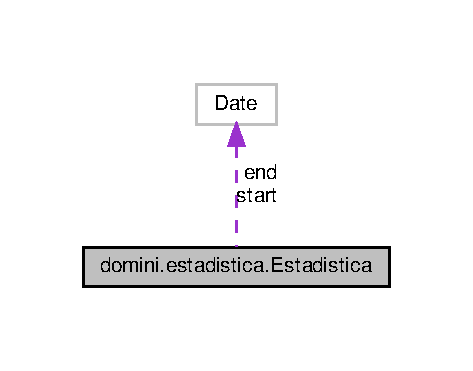
\includegraphics[width=227pt]{classdomini_1_1estadistica_1_1Estadistica__coll__graph}
\end{center}
\end{figure}
\subsection*{Public Member Functions}
\begin{DoxyCompactItemize}
\item 
\hyperlink{classdomini_1_1estadistica_1_1Estadistica_a16c37d85709413fd65f8dee111faed49}{Estadistica} ()
\begin{DoxyCompactList}\small\item\em Constructor de la classe Estadística. \end{DoxyCompactList}\item 
void \hyperlink{classdomini_1_1estadistica_1_1Estadistica_a6cac6971be817fd985afb8f3b6725464}{show\+\_\+estadistica} (String inp, String out)
\begin{DoxyCompactList}\small\item\em Mostrarà les estadístiques de la compressió \end{DoxyCompactList}\end{DoxyCompactItemize}
\subsection*{Package Attributes}
\begin{DoxyCompactItemize}
\item 
Date \hyperlink{classdomini_1_1estadistica_1_1Estadistica_aee0ae604272563ceab4e61392cbd343e}{start}
\item 
Date \hyperlink{classdomini_1_1estadistica_1_1Estadistica_ae99e664f0569e308009ec7ca32864006}{end}
\end{DoxyCompactItemize}
\subsection*{Private Member Functions}
\begin{DoxyCompactItemize}
\item 
\mbox{\Hypertarget{classdomini_1_1estadistica_1_1Estadistica_a7587e21e3f7f177afe0dd36483c8fe5d}\label{classdomini_1_1estadistica_1_1Estadistica_a7587e21e3f7f177afe0dd36483c8fe5d}} 
long {\bfseries time} (Date i, Date f)
\end{DoxyCompactItemize}


\subsection{Detailed Description}
Generació de les estadístiques durant la compressió 

\begin{DoxyAuthor}{Author}
Manel Aguilar 
\end{DoxyAuthor}


\subsection{Constructor \& Destructor Documentation}
\mbox{\Hypertarget{classdomini_1_1estadistica_1_1Estadistica_a16c37d85709413fd65f8dee111faed49}\label{classdomini_1_1estadistica_1_1Estadistica_a16c37d85709413fd65f8dee111faed49}} 
\index{domini\+::estadistica\+::\+Estadistica@{domini\+::estadistica\+::\+Estadistica}!Estadistica@{Estadistica}}
\index{Estadistica@{Estadistica}!domini\+::estadistica\+::\+Estadistica@{domini\+::estadistica\+::\+Estadistica}}
\subsubsection{\texorpdfstring{Estadistica()}{Estadistica()}}
{\footnotesize\ttfamily domini.\+estadistica.\+Estadistica.\+Estadistica (\begin{DoxyParamCaption}{ }\end{DoxyParamCaption})\hspace{0.3cm}{\ttfamily [inline]}}



Constructor de la classe Estadística. 

\begin{DoxyNote}{Note}
Generem l\textquotesingle{}Instancia d\textquotesingle{}inici de temps de compressió 
\end{DoxyNote}


\subsection{Member Function Documentation}
\mbox{\Hypertarget{classdomini_1_1estadistica_1_1Estadistica_a6cac6971be817fd985afb8f3b6725464}\label{classdomini_1_1estadistica_1_1Estadistica_a6cac6971be817fd985afb8f3b6725464}} 
\index{domini\+::estadistica\+::\+Estadistica@{domini\+::estadistica\+::\+Estadistica}!show\+\_\+estadistica@{show\+\_\+estadistica}}
\index{show\+\_\+estadistica@{show\+\_\+estadistica}!domini\+::estadistica\+::\+Estadistica@{domini\+::estadistica\+::\+Estadistica}}
\subsubsection{\texorpdfstring{show\+\_\+estadistica()}{show\_estadistica()}}
{\footnotesize\ttfamily public void domini.\+estadistica.\+Estadistica.\+show\+\_\+estadistica (\begin{DoxyParamCaption}\item[{String}]{inp,  }\item[{String}]{out }\end{DoxyParamCaption})\hspace{0.3cm}{\ttfamily [inline]}}



Mostrarà les estadístiques de la compressió 


\begin{DoxyParams}{Parameters}
{\em inp} & Path de l\textquotesingle{}arxiu que haviem de comprimir \\
\hline
{\em out} & Path de l\textquotesingle{}arxiu comprimit \\
\hline
\end{DoxyParams}


\subsection{Member Data Documentation}
\mbox{\Hypertarget{classdomini_1_1estadistica_1_1Estadistica_ae99e664f0569e308009ec7ca32864006}\label{classdomini_1_1estadistica_1_1Estadistica_ae99e664f0569e308009ec7ca32864006}} 
\index{domini\+::estadistica\+::\+Estadistica@{domini\+::estadistica\+::\+Estadistica}!end@{end}}
\index{end@{end}!domini\+::estadistica\+::\+Estadistica@{domini\+::estadistica\+::\+Estadistica}}
\subsubsection{\texorpdfstring{end}{end}}
{\footnotesize\ttfamily Date domini.\+estadistica.\+Estadistica.\+end\hspace{0.3cm}{\ttfamily [package]}}


\begin{DoxyParams}{Parameters}
{\em end} & Instancia del moment en que acabem la compressió \\
\hline
\end{DoxyParams}
\mbox{\Hypertarget{classdomini_1_1estadistica_1_1Estadistica_aee0ae604272563ceab4e61392cbd343e}\label{classdomini_1_1estadistica_1_1Estadistica_aee0ae604272563ceab4e61392cbd343e}} 
\index{domini\+::estadistica\+::\+Estadistica@{domini\+::estadistica\+::\+Estadistica}!start@{start}}
\index{start@{start}!domini\+::estadistica\+::\+Estadistica@{domini\+::estadistica\+::\+Estadistica}}
\subsubsection{\texorpdfstring{start}{start}}
{\footnotesize\ttfamily Date domini.\+estadistica.\+Estadistica.\+start\hspace{0.3cm}{\ttfamily [package]}}


\begin{DoxyParams}{Parameters}
{\em start} & Instancia del moment en que comencem la compressió \\
\hline
\end{DoxyParams}


The documentation for this class was generated from the following file\+:\begin{DoxyCompactItemize}
\item 
src/domini/estadistica/Estadistica.\+java\end{DoxyCompactItemize}

\hypertarget{classpersistencia_1_1input_1_1Input}{}\section{persistencia.\+input.\+Input Class Reference}
\label{classpersistencia_1_1input_1_1Input}\index{persistencia.\+input.\+Input@{persistencia.\+input.\+Input}}


Classe \hyperlink{classpersistencia_1_1input_1_1Input}{Input}.  


\subsection*{Public Member Functions}
\begin{DoxyCompactItemize}
\item 
\hyperlink{classpersistencia_1_1input_1_1Input_a9b30ef8d489a1fc5b4aa04a14474349a}{Input} (String path)
\begin{DoxyCompactList}\small\item\em Constructor de la classe. \end{DoxyCompactList}\item 
byte \hyperlink{classpersistencia_1_1input_1_1Input_a3fa5a378b2155a3022a4a4ef38d63a8e}{get\+Bits} (int num\+\_\+bits)
\item 
Array\+List$<$ Byte $>$ \hyperlink{classpersistencia_1_1input_1_1Input_a81e96a5ac3ca41b5001ffff9f9acc76a}{get\+More\+Bits} (int num\+\_\+bits)
\item 
boolean \hyperlink{classpersistencia_1_1input_1_1Input_af607cad1726ef15cf8e970dcbee74b68}{finished} ()
\item 
int \hyperlink{classpersistencia_1_1input_1_1Input_a3f0fc057e91430b81f5f2c92f91b8ed7}{out\+Of\+File} ()
\item 
String \hyperlink{classpersistencia_1_1input_1_1Input_a95e2068bd17e415f0487f8193f066160}{get\+Decode\+Alg} ()
\end{DoxyCompactItemize}


\subsection{Detailed Description}
Classe \hyperlink{classpersistencia_1_1input_1_1Input}{Input}. 

\begin{DoxyAuthor}{Author}

\end{DoxyAuthor}


\subsection{Constructor \& Destructor Documentation}
\mbox{\Hypertarget{classpersistencia_1_1input_1_1Input_a9b30ef8d489a1fc5b4aa04a14474349a}\label{classpersistencia_1_1input_1_1Input_a9b30ef8d489a1fc5b4aa04a14474349a}} 
\index{persistencia\+::input\+::\+Input@{persistencia\+::input\+::\+Input}!Input@{Input}}
\index{Input@{Input}!persistencia\+::input\+::\+Input@{persistencia\+::input\+::\+Input}}
\subsubsection{\texorpdfstring{Input()}{Input()}}
{\footnotesize\ttfamily persistencia.\+input.\+Input.\+Input (\begin{DoxyParamCaption}\item[{String}]{path }\end{DoxyParamCaption})\hspace{0.3cm}{\ttfamily [inline]}}



Constructor de la classe. 


\begin{DoxyParams}{Parameters}
{\em path} & Path de l\textquotesingle{}arxiu d\textquotesingle{}\hyperlink{classpersistencia_1_1input_1_1Input}{Input} \\
\hline
\end{DoxyParams}


\subsection{Member Function Documentation}
\mbox{\Hypertarget{classpersistencia_1_1input_1_1Input_af607cad1726ef15cf8e970dcbee74b68}\label{classpersistencia_1_1input_1_1Input_af607cad1726ef15cf8e970dcbee74b68}} 
\index{persistencia\+::input\+::\+Input@{persistencia\+::input\+::\+Input}!finished@{finished}}
\index{finished@{finished}!persistencia\+::input\+::\+Input@{persistencia\+::input\+::\+Input}}
\subsubsection{\texorpdfstring{finished()}{finished()}}
{\footnotesize\ttfamily public boolean persistencia.\+input.\+Input.\+finished (\begin{DoxyParamCaption}{ }\end{DoxyParamCaption})\hspace{0.3cm}{\ttfamily [inline]}}

\begin{DoxyReturn}{Returns}
Retorna si hem arribat al final de l\textquotesingle{}arxiu o no 
\end{DoxyReturn}
\mbox{\Hypertarget{classpersistencia_1_1input_1_1Input_a3fa5a378b2155a3022a4a4ef38d63a8e}\label{classpersistencia_1_1input_1_1Input_a3fa5a378b2155a3022a4a4ef38d63a8e}} 
\index{persistencia\+::input\+::\+Input@{persistencia\+::input\+::\+Input}!get\+Bits@{get\+Bits}}
\index{get\+Bits@{get\+Bits}!persistencia\+::input\+::\+Input@{persistencia\+::input\+::\+Input}}
\subsubsection{\texorpdfstring{get\+Bits()}{getBits()}}
{\footnotesize\ttfamily public byte persistencia.\+input.\+Input.\+get\+Bits (\begin{DoxyParamCaption}\item[{int}]{num\+\_\+bits }\end{DoxyParamCaption})\hspace{0.3cm}{\ttfamily [inline]}}


\begin{DoxyParams}{Parameters}
{\em num\+\_\+bits} & Nombre de bits que volem que ens retorni ( 1 $<$= num\+\_\+bits $<$= 8) \\
\hline
\end{DoxyParams}
\begin{DoxyReturn}{Returns}
Retorna un byte amb num\+\_\+bits bits valids 
\end{DoxyReturn}
\mbox{\Hypertarget{classpersistencia_1_1input_1_1Input_a95e2068bd17e415f0487f8193f066160}\label{classpersistencia_1_1input_1_1Input_a95e2068bd17e415f0487f8193f066160}} 
\index{persistencia\+::input\+::\+Input@{persistencia\+::input\+::\+Input}!get\+Decode\+Alg@{get\+Decode\+Alg}}
\index{get\+Decode\+Alg@{get\+Decode\+Alg}!persistencia\+::input\+::\+Input@{persistencia\+::input\+::\+Input}}
\subsubsection{\texorpdfstring{get\+Decode\+Alg()}{getDecodeAlg()}}
{\footnotesize\ttfamily public String persistencia.\+input.\+Input.\+get\+Decode\+Alg (\begin{DoxyParamCaption}{ }\end{DoxyParamCaption})\hspace{0.3cm}{\ttfamily [inline]}}

\begin{DoxyReturn}{Returns}
Retorna l\textquotesingle{}algoritme que hem d\textquotesingle{}emprar per la descompressio 
\end{DoxyReturn}
\mbox{\Hypertarget{classpersistencia_1_1input_1_1Input_a81e96a5ac3ca41b5001ffff9f9acc76a}\label{classpersistencia_1_1input_1_1Input_a81e96a5ac3ca41b5001ffff9f9acc76a}} 
\index{persistencia\+::input\+::\+Input@{persistencia\+::input\+::\+Input}!get\+More\+Bits@{get\+More\+Bits}}
\index{get\+More\+Bits@{get\+More\+Bits}!persistencia\+::input\+::\+Input@{persistencia\+::input\+::\+Input}}
\subsubsection{\texorpdfstring{get\+More\+Bits()}{getMoreBits()}}
{\footnotesize\ttfamily public Array\+List$<$ Byte $>$ persistencia.\+input.\+Input.\+get\+More\+Bits (\begin{DoxyParamCaption}\item[{int}]{num\+\_\+bits }\end{DoxyParamCaption})\hspace{0.3cm}{\ttfamily [inline]}}


\begin{DoxyParams}{Parameters}
{\em num\+\_\+bits} & Nombre de bits que volem que ens retorni \\
\hline
\end{DoxyParams}
\begin{DoxyReturn}{Returns}
Array\+List de Bytes amb num\+\_\+bits bits valids 
\end{DoxyReturn}
\mbox{\Hypertarget{classpersistencia_1_1input_1_1Input_a3f0fc057e91430b81f5f2c92f91b8ed7}\label{classpersistencia_1_1input_1_1Input_a3f0fc057e91430b81f5f2c92f91b8ed7}} 
\index{persistencia\+::input\+::\+Input@{persistencia\+::input\+::\+Input}!out\+Of\+File@{out\+Of\+File}}
\index{out\+Of\+File@{out\+Of\+File}!persistencia\+::input\+::\+Input@{persistencia\+::input\+::\+Input}}
\subsubsection{\texorpdfstring{out\+Of\+File()}{outOfFile()}}
{\footnotesize\ttfamily public int persistencia.\+input.\+Input.\+out\+Of\+File (\begin{DoxyParamCaption}{ }\end{DoxyParamCaption})\hspace{0.3cm}{\ttfamily [inline]}}

\begin{DoxyReturn}{Returns}
Retorna el nombre de bits que s\textquotesingle{}han intentat llegir però queden fora del fitxer 
\end{DoxyReturn}


The documentation for this class was generated from the following file\+:\begin{DoxyCompactItemize}
\item 
src/persistencia/input/Input.\+java\end{DoxyCompactItemize}

\hypertarget{classpersistencia_1_1input_1_1Input__Text}{}\section{persistencia.\+input.\+Input\+\_\+\+Text Class Reference}
\label{classpersistencia_1_1input_1_1Input__Text}\index{persistencia.\+input.\+Input\+\_\+\+Text@{persistencia.\+input.\+Input\+\_\+\+Text}}


Classe \hyperlink{classpersistencia_1_1input_1_1Input__Text}{Input\+\_\+\+Text}.  




Collaboration diagram for persistencia.\+input.\+Input\+\_\+\+Text\+:\nopagebreak
\begin{figure}[H]
\begin{center}
\leavevmode
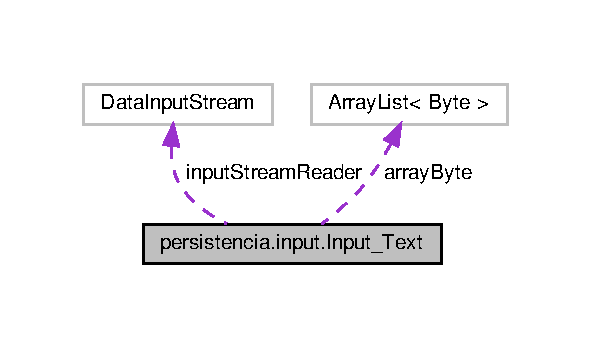
\includegraphics[width=284pt]{classpersistencia_1_1input_1_1Input__Text__coll__graph}
\end{center}
\end{figure}
\subsection*{Public Member Functions}
\begin{DoxyCompactItemize}
\item 
\hyperlink{classpersistencia_1_1input_1_1Input__Text_a9027dd15a85630115b38369358defd04}{Input\+\_\+\+Text} (String path)
\begin{DoxyCompactList}\small\item\em Constructor de la classe. \end{DoxyCompactList}\item 
byte \hyperlink{classpersistencia_1_1input_1_1Input__Text_a471f357f566d79f224a9cc51967f34ef}{get\+Bits} (int num\+\_\+bits)
\item 
Array\+List$<$ Byte $>$ \hyperlink{classpersistencia_1_1input_1_1Input__Text_a36c0224f7ac8f3a60a80bacc571dd3be}{get\+In} ()
\end{DoxyCompactItemize}
\subsection*{Package Attributes}
\begin{DoxyCompactItemize}
\item 
Array\+List$<$ Byte $>$ \hyperlink{classpersistencia_1_1input_1_1Input__Text_ab29b20f25abf37ab5fa9fd86e446fdf5}{array\+Byte}
\end{DoxyCompactItemize}
\subsection*{Private Member Functions}
\begin{DoxyCompactItemize}
\item 
\mbox{\Hypertarget{classpersistencia_1_1input_1_1Input__Text_a7a9380838f5fe9c753c1e94a8cf47437}\label{classpersistencia_1_1input_1_1Input__Text_a7a9380838f5fe9c753c1e94a8cf47437}} 
void \hyperlink{classpersistencia_1_1input_1_1Input__Text_a7a9380838f5fe9c753c1e94a8cf47437}{read} ()
\begin{DoxyCompactList}\small\item\em Llegeix bytes de l\textquotesingle{}arxiu. \end{DoxyCompactList}\end{DoxyCompactItemize}
\subsection*{Private Attributes}
\begin{DoxyCompactItemize}
\item 
Data\+Input\+Stream \hyperlink{classpersistencia_1_1input_1_1Input__Text_a032eea39e81853708f2c0d1358d08301}{input\+Stream\+Reader}
\item 
int \hyperlink{classpersistencia_1_1input_1_1Input__Text_a38dcfc8b8b79a8820e42f4ed6031ea01}{punter}
\item 
int \hyperlink{classpersistencia_1_1input_1_1Input__Text_a89dcd598f4620d041db312f0aa2ca19a}{pos}
\end{DoxyCompactItemize}


\subsection{Detailed Description}
Classe \hyperlink{classpersistencia_1_1input_1_1Input__Text}{Input\+\_\+\+Text}. 

\begin{DoxyAuthor}{Author}

\end{DoxyAuthor}


\subsection{Constructor \& Destructor Documentation}
\mbox{\Hypertarget{classpersistencia_1_1input_1_1Input__Text_a9027dd15a85630115b38369358defd04}\label{classpersistencia_1_1input_1_1Input__Text_a9027dd15a85630115b38369358defd04}} 
\index{persistencia\+::input\+::\+Input\+\_\+\+Text@{persistencia\+::input\+::\+Input\+\_\+\+Text}!Input\+\_\+\+Text@{Input\+\_\+\+Text}}
\index{Input\+\_\+\+Text@{Input\+\_\+\+Text}!persistencia\+::input\+::\+Input\+\_\+\+Text@{persistencia\+::input\+::\+Input\+\_\+\+Text}}
\subsubsection{\texorpdfstring{Input\+\_\+\+Text()}{Input\_Text()}}
{\footnotesize\ttfamily persistencia.\+input.\+Input\+\_\+\+Text.\+Input\+\_\+\+Text (\begin{DoxyParamCaption}\item[{String}]{path }\end{DoxyParamCaption})\hspace{0.3cm}{\ttfamily [inline]}}



Constructor de la classe. 


\begin{DoxyParams}{Parameters}
{\em path} & Path de l\textquotesingle{}arxiu a tractar \\
\hline
\end{DoxyParams}


\subsection{Member Function Documentation}
\mbox{\Hypertarget{classpersistencia_1_1input_1_1Input__Text_a471f357f566d79f224a9cc51967f34ef}\label{classpersistencia_1_1input_1_1Input__Text_a471f357f566d79f224a9cc51967f34ef}} 
\index{persistencia\+::input\+::\+Input\+\_\+\+Text@{persistencia\+::input\+::\+Input\+\_\+\+Text}!get\+Bits@{get\+Bits}}
\index{get\+Bits@{get\+Bits}!persistencia\+::input\+::\+Input\+\_\+\+Text@{persistencia\+::input\+::\+Input\+\_\+\+Text}}
\subsubsection{\texorpdfstring{get\+Bits()}{getBits()}}
{\footnotesize\ttfamily public byte persistencia.\+input.\+Input\+\_\+\+Text.\+get\+Bits (\begin{DoxyParamCaption}\item[{int}]{num\+\_\+bits }\end{DoxyParamCaption})\hspace{0.3cm}{\ttfamily [inline]}}


\begin{DoxyParams}{Parameters}
{\em num\+\_\+bits} & Especifica el nombre de bits que volem de l\textquotesingle{}input (num\+\_\+bits -\/$>$ \{0,8\}) \\
\hline
\end{DoxyParams}
\begin{DoxyReturn}{Returns}
Retorna un byte amb el nombre valid de bits que demanem 
\end{DoxyReturn}
\mbox{\Hypertarget{classpersistencia_1_1input_1_1Input__Text_a36c0224f7ac8f3a60a80bacc571dd3be}\label{classpersistencia_1_1input_1_1Input__Text_a36c0224f7ac8f3a60a80bacc571dd3be}} 
\index{persistencia\+::input\+::\+Input\+\_\+\+Text@{persistencia\+::input\+::\+Input\+\_\+\+Text}!get\+In@{get\+In}}
\index{get\+In@{get\+In}!persistencia\+::input\+::\+Input\+\_\+\+Text@{persistencia\+::input\+::\+Input\+\_\+\+Text}}
\subsubsection{\texorpdfstring{get\+In()}{getIn()}}
{\footnotesize\ttfamily public Array\+List$<$ Byte $>$ persistencia.\+input.\+Input\+\_\+\+Text.\+get\+In (\begin{DoxyParamCaption}{ }\end{DoxyParamCaption})\hspace{0.3cm}{\ttfamily [inline]}}

\begin{DoxyReturn}{Returns}
Retorna l\textquotesingle{}atribut de la classe 
\end{DoxyReturn}


\subsection{Member Data Documentation}
\mbox{\Hypertarget{classpersistencia_1_1input_1_1Input__Text_ab29b20f25abf37ab5fa9fd86e446fdf5}\label{classpersistencia_1_1input_1_1Input__Text_ab29b20f25abf37ab5fa9fd86e446fdf5}} 
\index{persistencia\+::input\+::\+Input\+\_\+\+Text@{persistencia\+::input\+::\+Input\+\_\+\+Text}!array\+Byte@{array\+Byte}}
\index{array\+Byte@{array\+Byte}!persistencia\+::input\+::\+Input\+\_\+\+Text@{persistencia\+::input\+::\+Input\+\_\+\+Text}}
\subsubsection{\texorpdfstring{array\+Byte}{arrayByte}}
{\footnotesize\ttfamily Array\+List$<$Byte$>$ persistencia.\+input.\+Input\+\_\+\+Text.\+array\+Byte\hspace{0.3cm}{\ttfamily [package]}}


\begin{DoxyParams}{Parameters}
{\em array\+Byte} & \\
\hline
\end{DoxyParams}
\mbox{\Hypertarget{classpersistencia_1_1input_1_1Input__Text_a032eea39e81853708f2c0d1358d08301}\label{classpersistencia_1_1input_1_1Input__Text_a032eea39e81853708f2c0d1358d08301}} 
\index{persistencia\+::input\+::\+Input\+\_\+\+Text@{persistencia\+::input\+::\+Input\+\_\+\+Text}!input\+Stream\+Reader@{input\+Stream\+Reader}}
\index{input\+Stream\+Reader@{input\+Stream\+Reader}!persistencia\+::input\+::\+Input\+\_\+\+Text@{persistencia\+::input\+::\+Input\+\_\+\+Text}}
\subsubsection{\texorpdfstring{input\+Stream\+Reader}{inputStreamReader}}
{\footnotesize\ttfamily Data\+Input\+Stream persistencia.\+input.\+Input\+\_\+\+Text.\+input\+Stream\+Reader\hspace{0.3cm}{\ttfamily [private]}}


\begin{DoxyParams}{Parameters}
{\em input\+Stream\+Reader} & \\
\hline
\end{DoxyParams}
\mbox{\Hypertarget{classpersistencia_1_1input_1_1Input__Text_a89dcd598f4620d041db312f0aa2ca19a}\label{classpersistencia_1_1input_1_1Input__Text_a89dcd598f4620d041db312f0aa2ca19a}} 
\index{persistencia\+::input\+::\+Input\+\_\+\+Text@{persistencia\+::input\+::\+Input\+\_\+\+Text}!pos@{pos}}
\index{pos@{pos}!persistencia\+::input\+::\+Input\+\_\+\+Text@{persistencia\+::input\+::\+Input\+\_\+\+Text}}
\subsubsection{\texorpdfstring{pos}{pos}}
{\footnotesize\ttfamily int persistencia.\+input.\+Input\+\_\+\+Text.\+pos\hspace{0.3cm}{\ttfamily [private]}}


\begin{DoxyParams}{Parameters}
{\em pos} & \\
\hline
\end{DoxyParams}
\mbox{\Hypertarget{classpersistencia_1_1input_1_1Input__Text_a38dcfc8b8b79a8820e42f4ed6031ea01}\label{classpersistencia_1_1input_1_1Input__Text_a38dcfc8b8b79a8820e42f4ed6031ea01}} 
\index{persistencia\+::input\+::\+Input\+\_\+\+Text@{persistencia\+::input\+::\+Input\+\_\+\+Text}!punter@{punter}}
\index{punter@{punter}!persistencia\+::input\+::\+Input\+\_\+\+Text@{persistencia\+::input\+::\+Input\+\_\+\+Text}}
\subsubsection{\texorpdfstring{punter}{punter}}
{\footnotesize\ttfamily int persistencia.\+input.\+Input\+\_\+\+Text.\+punter\hspace{0.3cm}{\ttfamily [private]}}


\begin{DoxyParams}{Parameters}
{\em punter} & \\
\hline
\end{DoxyParams}


The documentation for this class was generated from the following file\+:\begin{DoxyCompactItemize}
\item 
src/persistencia/input/Input\+\_\+\+Text.\+java\end{DoxyCompactItemize}

\hypertarget{classdomini_1_1utils_1_1IntorByte}{}\section{domini.\+utils.\+Intor\+Byte Class Reference}
\label{classdomini_1_1utils_1_1IntorByte}\index{domini.\+utils.\+Intor\+Byte@{domini.\+utils.\+Intor\+Byte}}


Classe auxiliar per l\textquotesingle{}algorisme L\+Z\+SS.  


\subsection*{Public Member Functions}
\begin{DoxyCompactItemize}
\item 
\hyperlink{classdomini_1_1utils_1_1IntorByte_ac2bae675cf6c4d8880acedeefaf24060}{Intor\+Byte} (boolean b)
\begin{DoxyCompactList}\small\item\em El constructor. \end{DoxyCompactList}\item 
void \hyperlink{classdomini_1_1utils_1_1IntorByte_a01c26f8a3a94b2bc31fda2f5989fca00}{Set\+Despl} (int \hyperlink{classdomini_1_1utils_1_1IntorByte_a83872b8acc9ab187acbc2175d5bf320e}{despl})
\begin{DoxyCompactList}\small\item\em Mètode per establir un possible despl. \end{DoxyCompactList}\item 
void \hyperlink{classdomini_1_1utils_1_1IntorByte_a2371fca6d26baf4098466dbb3089052d}{Set\+Mida} (int \hyperlink{classdomini_1_1utils_1_1IntorByte_a6dd2ad21efcfb2bcfff716f5e04794d9}{mida})
\begin{DoxyCompactList}\small\item\em Mètode per establir una possible mida. \end{DoxyCompactList}\item 
void \hyperlink{classdomini_1_1utils_1_1IntorByte_a02677743722d43ce96904e03eb82f25b}{Set\+Byte} (byte c)
\begin{DoxyCompactList}\small\item\em Mètode per establir un possible byte. \end{DoxyCompactList}\item 
int \hyperlink{classdomini_1_1utils_1_1IntorByte_a5d99bc2397d586c3e3319eadf7f23e4d}{Get\+Despl} ()
\begin{DoxyCompactList}\small\item\em Mètode per obtenir un possible despl. \end{DoxyCompactList}\item 
int \hyperlink{classdomini_1_1utils_1_1IntorByte_abccf2f9cda2f62acdf0c1342f9acdead}{Get\+Mida} ()
\begin{DoxyCompactList}\small\item\em Mètode per obtenir una possible mida. \end{DoxyCompactList}\item 
byte \hyperlink{classdomini_1_1utils_1_1IntorByte_afd907b7001011bbca374605fb11491f4}{Get\+Byte} ()
\begin{DoxyCompactList}\small\item\em Mètode per obtenir un possible byte. \end{DoxyCompactList}\item 
boolean \hyperlink{classdomini_1_1utils_1_1IntorByte_a4fcfaf967d0c82b8147d632da4e238d0}{Is\+Intor\+Byte} ()
\begin{DoxyCompactList}\small\item\em Mètode per saber si és un byte o 2 int\textquotesingle{}s. \end{DoxyCompactList}\end{DoxyCompactItemize}
\subsection*{Private Attributes}
\begin{DoxyCompactItemize}
\item 
boolean \hyperlink{classdomini_1_1utils_1_1IntorByte_aee013881ecae778d25cab7c0b7655528}{intobyte}
\item 
byte \hyperlink{classdomini_1_1utils_1_1IntorByte_adbb2e8c31ead2f27d85ff39683b9a8a7}{caracter}
\item 
int \hyperlink{classdomini_1_1utils_1_1IntorByte_a83872b8acc9ab187acbc2175d5bf320e}{despl}
\item 
int \hyperlink{classdomini_1_1utils_1_1IntorByte_a6dd2ad21efcfb2bcfff716f5e04794d9}{mida}
\end{DoxyCompactItemize}


\subsection{Detailed Description}
Classe auxiliar per l\textquotesingle{}algorisme L\+Z\+SS. 

En aquesta classe es tracta de construir un objecte per obtenir una unitat mínima per al descompressor.

\begin{DoxyAuthor}{Author}
Manel Aguilar 
\end{DoxyAuthor}


\subsection{Constructor \& Destructor Documentation}
\mbox{\Hypertarget{classdomini_1_1utils_1_1IntorByte_ac2bae675cf6c4d8880acedeefaf24060}\label{classdomini_1_1utils_1_1IntorByte_ac2bae675cf6c4d8880acedeefaf24060}} 
\index{domini\+::utils\+::\+Intor\+Byte@{domini\+::utils\+::\+Intor\+Byte}!Intor\+Byte@{Intor\+Byte}}
\index{Intor\+Byte@{Intor\+Byte}!domini\+::utils\+::\+Intor\+Byte@{domini\+::utils\+::\+Intor\+Byte}}
\subsubsection{\texorpdfstring{Intor\+Byte()}{IntorByte()}}
{\footnotesize\ttfamily domini.\+utils.\+Intor\+Byte.\+Intor\+Byte (\begin{DoxyParamCaption}\item[{boolean}]{b }\end{DoxyParamCaption})\hspace{0.3cm}{\ttfamily [inline]}}



El constructor. 


\begin{DoxyParams}{Parameters}
{\em b} & Si és true es un byte, si és false, són dos int\textquotesingle{}s. \\
\hline
\end{DoxyParams}

\begin{DoxyCode}
38    \{
39       \hyperlink{classdomini_1_1utils_1_1IntorByte_aee013881ecae778d25cab7c0b7655528}{intobyte} = b;
40    \}
\end{DoxyCode}


\subsection{Member Function Documentation}
\mbox{\Hypertarget{classdomini_1_1utils_1_1IntorByte_afd907b7001011bbca374605fb11491f4}\label{classdomini_1_1utils_1_1IntorByte_afd907b7001011bbca374605fb11491f4}} 
\index{domini\+::utils\+::\+Intor\+Byte@{domini\+::utils\+::\+Intor\+Byte}!Get\+Byte@{Get\+Byte}}
\index{Get\+Byte@{Get\+Byte}!domini\+::utils\+::\+Intor\+Byte@{domini\+::utils\+::\+Intor\+Byte}}
\subsubsection{\texorpdfstring{Get\+Byte()}{GetByte()}}
{\footnotesize\ttfamily public byte domini.\+utils.\+Intor\+Byte.\+Get\+Byte (\begin{DoxyParamCaption}{ }\end{DoxyParamCaption})\hspace{0.3cm}{\ttfamily [inline]}}



Mètode per obtenir un possible byte. 

\begin{DoxyReturn}{Returns}
valor del atribut caracter. 
\end{DoxyReturn}

\begin{DoxyCode}
98    \{
99       \textcolor{keywordflow}{return} \hyperlink{classdomini_1_1utils_1_1IntorByte_adbb2e8c31ead2f27d85ff39683b9a8a7}{caracter};
100    \}
\end{DoxyCode}
\mbox{\Hypertarget{classdomini_1_1utils_1_1IntorByte_a5d99bc2397d586c3e3319eadf7f23e4d}\label{classdomini_1_1utils_1_1IntorByte_a5d99bc2397d586c3e3319eadf7f23e4d}} 
\index{domini\+::utils\+::\+Intor\+Byte@{domini\+::utils\+::\+Intor\+Byte}!Get\+Despl@{Get\+Despl}}
\index{Get\+Despl@{Get\+Despl}!domini\+::utils\+::\+Intor\+Byte@{domini\+::utils\+::\+Intor\+Byte}}
\subsubsection{\texorpdfstring{Get\+Despl()}{GetDespl()}}
{\footnotesize\ttfamily public int domini.\+utils.\+Intor\+Byte.\+Get\+Despl (\begin{DoxyParamCaption}{ }\end{DoxyParamCaption})\hspace{0.3cm}{\ttfamily [inline]}}



Mètode per obtenir un possible despl. 

\begin{DoxyReturn}{Returns}
valor del atribut despl. 
\end{DoxyReturn}

\begin{DoxyCode}
78    \{
79       \textcolor{keywordflow}{return} \hyperlink{classdomini_1_1utils_1_1IntorByte_a83872b8acc9ab187acbc2175d5bf320e}{despl};
80    \}
\end{DoxyCode}
\mbox{\Hypertarget{classdomini_1_1utils_1_1IntorByte_abccf2f9cda2f62acdf0c1342f9acdead}\label{classdomini_1_1utils_1_1IntorByte_abccf2f9cda2f62acdf0c1342f9acdead}} 
\index{domini\+::utils\+::\+Intor\+Byte@{domini\+::utils\+::\+Intor\+Byte}!Get\+Mida@{Get\+Mida}}
\index{Get\+Mida@{Get\+Mida}!domini\+::utils\+::\+Intor\+Byte@{domini\+::utils\+::\+Intor\+Byte}}
\subsubsection{\texorpdfstring{Get\+Mida()}{GetMida()}}
{\footnotesize\ttfamily public int domini.\+utils.\+Intor\+Byte.\+Get\+Mida (\begin{DoxyParamCaption}{ }\end{DoxyParamCaption})\hspace{0.3cm}{\ttfamily [inline]}}



Mètode per obtenir una possible mida. 

\begin{DoxyReturn}{Returns}
valor del atribut mida. 
\end{DoxyReturn}

\begin{DoxyCode}
88    \{
89       \textcolor{keywordflow}{return} \hyperlink{classdomini_1_1utils_1_1IntorByte_a6dd2ad21efcfb2bcfff716f5e04794d9}{mida};
90    \}
\end{DoxyCode}
\mbox{\Hypertarget{classdomini_1_1utils_1_1IntorByte_a4fcfaf967d0c82b8147d632da4e238d0}\label{classdomini_1_1utils_1_1IntorByte_a4fcfaf967d0c82b8147d632da4e238d0}} 
\index{domini\+::utils\+::\+Intor\+Byte@{domini\+::utils\+::\+Intor\+Byte}!Is\+Intor\+Byte@{Is\+Intor\+Byte}}
\index{Is\+Intor\+Byte@{Is\+Intor\+Byte}!domini\+::utils\+::\+Intor\+Byte@{domini\+::utils\+::\+Intor\+Byte}}
\subsubsection{\texorpdfstring{Is\+Intor\+Byte()}{IsIntorByte()}}
{\footnotesize\ttfamily public boolean domini.\+utils.\+Intor\+Byte.\+Is\+Intor\+Byte (\begin{DoxyParamCaption}{ }\end{DoxyParamCaption})\hspace{0.3cm}{\ttfamily [inline]}}



Mètode per saber si és un byte o 2 int\textquotesingle{}s. 

\begin{DoxyReturn}{Returns}
valor del atribut intobyte. 
\end{DoxyReturn}

\begin{DoxyCode}
108    \{
109       \textcolor{keywordflow}{return} \hyperlink{classdomini_1_1utils_1_1IntorByte_aee013881ecae778d25cab7c0b7655528}{intobyte};
110    \}
\end{DoxyCode}
\mbox{\Hypertarget{classdomini_1_1utils_1_1IntorByte_a02677743722d43ce96904e03eb82f25b}\label{classdomini_1_1utils_1_1IntorByte_a02677743722d43ce96904e03eb82f25b}} 
\index{domini\+::utils\+::\+Intor\+Byte@{domini\+::utils\+::\+Intor\+Byte}!Set\+Byte@{Set\+Byte}}
\index{Set\+Byte@{Set\+Byte}!domini\+::utils\+::\+Intor\+Byte@{domini\+::utils\+::\+Intor\+Byte}}
\subsubsection{\texorpdfstring{Set\+Byte()}{SetByte()}}
{\footnotesize\ttfamily public void domini.\+utils.\+Intor\+Byte.\+Set\+Byte (\begin{DoxyParamCaption}\item[{byte}]{c }\end{DoxyParamCaption})\hspace{0.3cm}{\ttfamily [inline]}}



Mètode per establir un possible byte. 


\begin{DoxyParams}{Parameters}
{\em c} & Valor que volem posar al atribut caracter. \\
\hline
\end{DoxyParams}

\begin{DoxyCode}
68    \{
69       \hyperlink{classdomini_1_1utils_1_1IntorByte_adbb2e8c31ead2f27d85ff39683b9a8a7}{caracter} = c;
70    \}
\end{DoxyCode}
\mbox{\Hypertarget{classdomini_1_1utils_1_1IntorByte_a01c26f8a3a94b2bc31fda2f5989fca00}\label{classdomini_1_1utils_1_1IntorByte_a01c26f8a3a94b2bc31fda2f5989fca00}} 
\index{domini\+::utils\+::\+Intor\+Byte@{domini\+::utils\+::\+Intor\+Byte}!Set\+Despl@{Set\+Despl}}
\index{Set\+Despl@{Set\+Despl}!domini\+::utils\+::\+Intor\+Byte@{domini\+::utils\+::\+Intor\+Byte}}
\subsubsection{\texorpdfstring{Set\+Despl()}{SetDespl()}}
{\footnotesize\ttfamily public void domini.\+utils.\+Intor\+Byte.\+Set\+Despl (\begin{DoxyParamCaption}\item[{int}]{despl }\end{DoxyParamCaption})\hspace{0.3cm}{\ttfamily [inline]}}



Mètode per establir un possible despl. 


\begin{DoxyParams}{Parameters}
{\em despl} & Valor que volem posar al atribut despl. \\
\hline
\end{DoxyParams}

\begin{DoxyCode}
48    \{
49       this.\hyperlink{classdomini_1_1utils_1_1IntorByte_a83872b8acc9ab187acbc2175d5bf320e}{despl} = \hyperlink{classdomini_1_1utils_1_1IntorByte_a83872b8acc9ab187acbc2175d5bf320e}{despl};
50    \}
\end{DoxyCode}
\mbox{\Hypertarget{classdomini_1_1utils_1_1IntorByte_a2371fca6d26baf4098466dbb3089052d}\label{classdomini_1_1utils_1_1IntorByte_a2371fca6d26baf4098466dbb3089052d}} 
\index{domini\+::utils\+::\+Intor\+Byte@{domini\+::utils\+::\+Intor\+Byte}!Set\+Mida@{Set\+Mida}}
\index{Set\+Mida@{Set\+Mida}!domini\+::utils\+::\+Intor\+Byte@{domini\+::utils\+::\+Intor\+Byte}}
\subsubsection{\texorpdfstring{Set\+Mida()}{SetMida()}}
{\footnotesize\ttfamily public void domini.\+utils.\+Intor\+Byte.\+Set\+Mida (\begin{DoxyParamCaption}\item[{int}]{mida }\end{DoxyParamCaption})\hspace{0.3cm}{\ttfamily [inline]}}



Mètode per establir una possible mida. 


\begin{DoxyParams}{Parameters}
{\em mida} & Valor que volem posar al atribut mida. \\
\hline
\end{DoxyParams}

\begin{DoxyCode}
58    \{
59       this.\hyperlink{classdomini_1_1utils_1_1IntorByte_a6dd2ad21efcfb2bcfff716f5e04794d9}{mida} = \hyperlink{classdomini_1_1utils_1_1IntorByte_a6dd2ad21efcfb2bcfff716f5e04794d9}{mida};
60    \}
\end{DoxyCode}


\subsection{Member Data Documentation}
\mbox{\Hypertarget{classdomini_1_1utils_1_1IntorByte_adbb2e8c31ead2f27d85ff39683b9a8a7}\label{classdomini_1_1utils_1_1IntorByte_adbb2e8c31ead2f27d85ff39683b9a8a7}} 
\index{domini\+::utils\+::\+Intor\+Byte@{domini\+::utils\+::\+Intor\+Byte}!caracter@{caracter}}
\index{caracter@{caracter}!domini\+::utils\+::\+Intor\+Byte@{domini\+::utils\+::\+Intor\+Byte}}
\subsubsection{\texorpdfstring{caracter}{caracter}}
{\footnotesize\ttfamily byte domini.\+utils.\+Intor\+Byte.\+caracter\hspace{0.3cm}{\ttfamily [private]}}


\begin{DoxyParams}{Parameters}
{\em caracter} & byte on té valor si intochar és true. \\
\hline
\end{DoxyParams}
\mbox{\Hypertarget{classdomini_1_1utils_1_1IntorByte_a83872b8acc9ab187acbc2175d5bf320e}\label{classdomini_1_1utils_1_1IntorByte_a83872b8acc9ab187acbc2175d5bf320e}} 
\index{domini\+::utils\+::\+Intor\+Byte@{domini\+::utils\+::\+Intor\+Byte}!despl@{despl}}
\index{despl@{despl}!domini\+::utils\+::\+Intor\+Byte@{domini\+::utils\+::\+Intor\+Byte}}
\subsubsection{\texorpdfstring{despl}{despl}}
{\footnotesize\ttfamily int domini.\+utils.\+Intor\+Byte.\+despl\hspace{0.3cm}{\ttfamily [private]}}


\begin{DoxyParams}{Parameters}
{\em despl} & Té el valor d\textquotesingle{}un int si intochar és false. \\
\hline
\end{DoxyParams}
\mbox{\Hypertarget{classdomini_1_1utils_1_1IntorByte_aee013881ecae778d25cab7c0b7655528}\label{classdomini_1_1utils_1_1IntorByte_aee013881ecae778d25cab7c0b7655528}} 
\index{domini\+::utils\+::\+Intor\+Byte@{domini\+::utils\+::\+Intor\+Byte}!intobyte@{intobyte}}
\index{intobyte@{intobyte}!domini\+::utils\+::\+Intor\+Byte@{domini\+::utils\+::\+Intor\+Byte}}
\subsubsection{\texorpdfstring{intobyte}{intobyte}}
{\footnotesize\ttfamily boolean domini.\+utils.\+Intor\+Byte.\+intobyte\hspace{0.3cm}{\ttfamily [private]}}


\begin{DoxyParams}{Parameters}
{\em intobyte} & Bool on false són 2 int\textquotesingle{}s i true és un byte. \\
\hline
\end{DoxyParams}
\mbox{\Hypertarget{classdomini_1_1utils_1_1IntorByte_a6dd2ad21efcfb2bcfff716f5e04794d9}\label{classdomini_1_1utils_1_1IntorByte_a6dd2ad21efcfb2bcfff716f5e04794d9}} 
\index{domini\+::utils\+::\+Intor\+Byte@{domini\+::utils\+::\+Intor\+Byte}!mida@{mida}}
\index{mida@{mida}!domini\+::utils\+::\+Intor\+Byte@{domini\+::utils\+::\+Intor\+Byte}}
\subsubsection{\texorpdfstring{mida}{mida}}
{\footnotesize\ttfamily int domini.\+utils.\+Intor\+Byte.\+mida\hspace{0.3cm}{\ttfamily [private]}}


\begin{DoxyParams}{Parameters}
{\em mida} & Té el valor d\textquotesingle{}un int si intochar és false. \\
\hline
\end{DoxyParams}


The documentation for this class was generated from the following file\+:\begin{DoxyCompactItemize}
\item 
src/domini/utils/\hyperlink{IntorByte_8java}{Intor\+Byte.\+java}\end{DoxyCompactItemize}

\hypertarget{classdomini_1_1algorithm_1_1JPEG}{}\section{domini.\+algorithm.\+J\+P\+EG Class Reference}
\label{classdomini_1_1algorithm_1_1JPEG}\index{domini.\+algorithm.\+J\+P\+EG@{domini.\+algorithm.\+J\+P\+EG}}


Compressió i descompressió pel mètode \hyperlink{classdomini_1_1algorithm_1_1JPEG}{J\+P\+EG}.  




Inheritance diagram for domini.\+algorithm.\+J\+P\+EG\+:
% FIG 0


Collaboration diagram for domini.\+algorithm.\+J\+P\+EG\+:
% FIG 1
\subsection*{Public Member Functions}
\begin{DoxyCompactItemize}
\item 
\hyperlink{classdomini_1_1algorithm_1_1JPEG_ac489916de8505f11b6e29c7206baf3c7}{J\+P\+EG} (String path, boolean b)
\begin{DoxyCompactList}\small\item\em Constructor de la classe. \end{DoxyCompactList}\item 
\hyperlink{classdomini_1_1algorithm_1_1JPEG_ade39a15f3c5722b4975746fcee6ad364}{J\+P\+EG} (boolean b)
\begin{DoxyCompactList}\small\item\em Constructor de la classe. \end{DoxyCompactList}\item 
void \hyperlink{classdomini_1_1algorithm_1_1JPEG_a860d6166ef8edc40b0ffb61942589e5d}{reset\+Quality} (int q)
\begin{DoxyCompactList}\small\item\em Construeix la matriu de quantització a partir de la qualitat. \end{DoxyCompactList}\item 
void \hyperlink{classdomini_1_1algorithm_1_1JPEG_a753bf49f2c8bde9e54464b21a1bcb2d8}{Compressor} ()
\begin{DoxyCompactList}\small\item\em Comprimim una imatge amb l\textquotesingle{}algoritme \hyperlink{classdomini_1_1algorithm_1_1JPEG}{J\+P\+EG}. \end{DoxyCompactList}\item 
void \hyperlink{classdomini_1_1algorithm_1_1JPEG_accca347e84e41b254d1f4a7bbdf2201a}{Decompressor} ()
\begin{DoxyCompactList}\small\item\em Desomprimim una imatge amb l\textquotesingle{}algoritme \hyperlink{classdomini_1_1algorithm_1_1JPEG}{J\+P\+EG}. \end{DoxyCompactList}\end{DoxyCompactItemize}
\subsection*{Package Attributes}
\begin{DoxyCompactItemize}
\item 
\hyperlink{classHuffman}{Huffman} \hyperlink{classdomini_1_1algorithm_1_1JPEG_aacc6445baa7819e3f9139ffb78e0b8f4}{huff}
\end{DoxyCompactItemize}
\subsection*{Static Private Member Functions}
\begin{DoxyCompactItemize}
\item 
static int \hyperlink{classdomini_1_1algorithm_1_1JPEG_aa9c52789d61d5eebdeb13ee39f8e817d}{round} (double x)
\begin{DoxyCompactList}\small\item\em Arrodoneix un número real. \end{DoxyCompactList}\item 
static double \hyperlink{classdomini_1_1algorithm_1_1JPEG_af86bdbb6b6f5671abff6bc6bd5f6349d}{force255} (double x)
\begin{DoxyCompactList}\small\item\em és la funcí alfa de D\+CT. \end{DoxyCompactList}\item 
static double \hyperlink{classdomini_1_1algorithm_1_1JPEG_a058b0ee7eb44bbaec4078b5fc32c5107}{alpha} (int x)
\item 
static void \hyperlink{classdomini_1_1algorithm_1_1JPEG_a367e6d1e6543bf3d8c847aae36f4b6bf}{discrete\+\_\+cosine\+\_\+transform} (double\mbox{[}$\,$\mbox{]}\mbox{[}$\,$\mbox{]} mat1)
\begin{DoxyCompactList}\small\item\em aplica discrete cosine transform (D\+CT) a una matriu 8x8 \end{DoxyCompactList}\item 
static void \hyperlink{classdomini_1_1algorithm_1_1JPEG_a3a6e16b0ee34746e4b0118ed9107bd75}{inverse\+\_\+discrete\+\_\+cosine\+\_\+transform} (double\mbox{[}$\,$\mbox{]}\mbox{[}$\,$\mbox{]} mat1)
\begin{DoxyCompactList}\small\item\em aplica discrete cosine transform (D\+CT) inversa a una matriu 8x8 \end{DoxyCompactList}\item 
static int \hyperlink{classdomini_1_1algorithm_1_1JPEG_a0f897c6c525d81551539df1eb8db7e12}{get\+\_\+entropy1\+\_\+code} (int runlength, int size)
\begin{DoxyCompactList}\small\item\em codifica runlength i size en el simbol1 de Entropy Coding \end{DoxyCompactList}\item 
static int \hyperlink{classdomini_1_1algorithm_1_1JPEG_ac58cb434a7acfd90fc8e548fd7c00ae2}{get\+\_\+runlength\+\_\+from\+\_\+entropy1} (int code)
\begin{DoxyCompactList}\small\item\em retorna el runlength codificat en un simbol1 de Entropy Coding \end{DoxyCompactList}\item 
static int \hyperlink{classdomini_1_1algorithm_1_1JPEG_a8d1005fb7833d36a064afb1c5e15bbd3}{get\+\_\+size\+\_\+from\+\_\+entropy1} (int code)
\item 
static int \hyperlink{classdomini_1_1algorithm_1_1JPEG_aa9bc9bee7181efee254be843e23ee2c6}{get\+\_\+entropy2\+\_\+size} (int value)
\begin{DoxyCompactList}\small\item\em codifica value en el symbol2 de Entropy Coding i en retorna la mida \end{DoxyCompactList}\item 
static int \hyperlink{classdomini_1_1algorithm_1_1JPEG_a0ccbcda5311dc96a30e5cb7f2a5b95b5}{get\+\_\+entropy2\+\_\+code} (int value)
\begin{DoxyCompactList}\small\item\em retorna la codifiacació en el simbol2 de Entropy Coding d\textquotesingle{}un cert valor \end{DoxyCompactList}\item 
static int \hyperlink{classdomini_1_1algorithm_1_1JPEG_a41c69fe2e29999dd17a555859df22530}{get\+\_\+value\+\_\+from\+\_\+entropy2} (int code, int size)
\begin{DoxyCompactList}\small\item\em retorna el valor codificat en un codi d\textquotesingle{}una determinada mida \end{DoxyCompactList}\end{DoxyCompactItemize}
\subsection*{Private Attributes}
\begin{DoxyCompactItemize}
\item 
int \mbox{[}$\,$\mbox{]}\mbox{[}$\,$\mbox{]} \hyperlink{classdomini_1_1algorithm_1_1JPEG_a7c95eb140dbe185a31b402d48ec17a66}{quantization\+\_\+matrix} = null
\item 
int \hyperlink{classdomini_1_1algorithm_1_1JPEG_ae80176d5ff56e613643db55e21c513da}{quality}
\end{DoxyCompactItemize}
\subsection*{Static Private Attributes}
\begin{DoxyCompactItemize}
\item 
static int \mbox{[}$\,$\mbox{]} \hyperlink{classdomini_1_1algorithm_1_1JPEG_a7d3829cbffd758c087341a8da13dd2ca}{zig\+Zag\+\_\+X}
\item 
static int \mbox{[}$\,$\mbox{]} \hyperlink{classdomini_1_1algorithm_1_1JPEG_ad886d8aa00a40cb151b446534f0d1bcc}{zig\+Zag\+\_\+Y}
\item 
static int \mbox{[}$\,$\mbox{]}\mbox{[}$\,$\mbox{]} \hyperlink{classdomini_1_1algorithm_1_1JPEG_a1f91c0bad6cfd3ac22bec68bc28564c5}{base\+\_\+quantization\+\_\+matrix}
\end{DoxyCompactItemize}
\subsection*{Additional Inherited Members}


\subsection{Detailed Description}
Compressió i descompressió pel mètode \hyperlink{classdomini_1_1algorithm_1_1JPEG}{J\+P\+EG}. 

\begin{DoxyAuthor}{Author}
Joan Lapeyra Amat 
\end{DoxyAuthor}


\subsection{Constructor \& Destructor Documentation}
\mbox{\Hypertarget{classdomini_1_1algorithm_1_1JPEG_ac489916de8505f11b6e29c7206baf3c7}\label{classdomini_1_1algorithm_1_1JPEG_ac489916de8505f11b6e29c7206baf3c7}} 
\index{domini\+::algorithm\+::\+J\+P\+EG@{domini\+::algorithm\+::\+J\+P\+EG}!J\+P\+EG@{J\+P\+EG}}
\index{J\+P\+EG@{J\+P\+EG}!domini\+::algorithm\+::\+J\+P\+EG@{domini\+::algorithm\+::\+J\+P\+EG}}
\subsubsection{\texorpdfstring{J\+P\+E\+G()}{JPEG()}\hspace{0.1cm}{\footnotesize\ttfamily [1/2]}}
{\footnotesize\ttfamily domini.\+algorithm.\+J\+P\+E\+G.\+J\+P\+EG (\begin{DoxyParamCaption}\item[{String}]{path,  }\item[{boolean}]{b }\end{DoxyParamCaption})\hspace{0.3cm}{\ttfamily [inline]}}



Constructor de la classe. 


\begin{DoxyParams}{Parameters}
{\em path} & Path de sortida \\
\hline
{\em b} & False si estas comprimint, True si estas descomprimint \\
\hline
\end{DoxyParams}

\begin{DoxyCode}
28                                         \{
29         super(path, b);
30         \textcolor{keywordflow}{if} (!b) \{
31             \hyperlink{classdomini_1_1algorithm_1_1Algorithm_a4de9955411c656325adc391ef570c082}{Output}.\hyperlink{classpersistencia_1_1output_1_1Ctrl__Output_ae6d6857910a023982900ddc857b891f0}{addMetadata}(\textcolor{stringliteral}{"jpeg"});
32         \}
33         \hyperlink{classdomini_1_1algorithm_1_1JPEG_aacc6445baa7819e3f9139ffb78e0b8f4}{huff} = \textcolor{keyword}{new} \hyperlink{classHuffman}{Huffman}();
34     \}
\end{DoxyCode}
\mbox{\Hypertarget{classdomini_1_1algorithm_1_1JPEG_ade39a15f3c5722b4975746fcee6ad364}\label{classdomini_1_1algorithm_1_1JPEG_ade39a15f3c5722b4975746fcee6ad364}} 
\index{domini\+::algorithm\+::\+J\+P\+EG@{domini\+::algorithm\+::\+J\+P\+EG}!J\+P\+EG@{J\+P\+EG}}
\index{J\+P\+EG@{J\+P\+EG}!domini\+::algorithm\+::\+J\+P\+EG@{domini\+::algorithm\+::\+J\+P\+EG}}
\subsubsection{\texorpdfstring{J\+P\+E\+G()}{JPEG()}\hspace{0.1cm}{\footnotesize\ttfamily [2/2]}}
{\footnotesize\ttfamily domini.\+algorithm.\+J\+P\+E\+G.\+J\+P\+EG (\begin{DoxyParamCaption}\item[{boolean}]{b }\end{DoxyParamCaption})\hspace{0.3cm}{\ttfamily [inline]}}



Constructor de la classe. 


\begin{DoxyParams}{Parameters}
{\em b} & False si estas comprimint, True si estas descomprimint \\
\hline
\end{DoxyParams}
\begin{DoxyNote}{Note}
Es continua escrivint al fitxer que s\textquotesingle{}estava escrivint 
\end{DoxyNote}

\begin{DoxyCode}
41                            \{
42         super(b);
43         \textcolor{keywordflow}{if} (!b) \{
44             \hyperlink{classdomini_1_1algorithm_1_1Algorithm_a4de9955411c656325adc391ef570c082}{Output}.\hyperlink{classpersistencia_1_1output_1_1Ctrl__Output_ae6d6857910a023982900ddc857b891f0}{addMetadata}(\textcolor{stringliteral}{"jpeg"});
45         \}
46         \hyperlink{classdomini_1_1algorithm_1_1JPEG_aacc6445baa7819e3f9139ffb78e0b8f4}{huff} = \textcolor{keyword}{new} \hyperlink{classHuffman}{Huffman}();
47     \}
\end{DoxyCode}


\subsection{Member Function Documentation}
\mbox{\Hypertarget{classdomini_1_1algorithm_1_1JPEG_a058b0ee7eb44bbaec4078b5fc32c5107}\label{classdomini_1_1algorithm_1_1JPEG_a058b0ee7eb44bbaec4078b5fc32c5107}} 
\index{domini\+::algorithm\+::\+J\+P\+EG@{domini\+::algorithm\+::\+J\+P\+EG}!alpha@{alpha}}
\index{alpha@{alpha}!domini\+::algorithm\+::\+J\+P\+EG@{domini\+::algorithm\+::\+J\+P\+EG}}
\subsubsection{\texorpdfstring{alpha()}{alpha()}}
{\footnotesize\ttfamily static double domini.\+algorithm.\+J\+P\+E\+G.\+alpha (\begin{DoxyParamCaption}\item[{int}]{x }\end{DoxyParamCaption})\hspace{0.3cm}{\ttfamily [inline]}, {\ttfamily [static]}, {\ttfamily [private]}}


\begin{DoxyCode}
173                                        \{ \textcolor{comment}{// only used in discrete\_cosine\_transform}
174         \textcolor{keywordflow}{if} (x == 0) \textcolor{keywordflow}{return} 1.0 / Math.sqrt(2);
175         \textcolor{keywordflow}{return} 1.0;
176     \}
\end{DoxyCode}
\mbox{\Hypertarget{classdomini_1_1algorithm_1_1JPEG_a753bf49f2c8bde9e54464b21a1bcb2d8}\label{classdomini_1_1algorithm_1_1JPEG_a753bf49f2c8bde9e54464b21a1bcb2d8}} 
\index{domini\+::algorithm\+::\+J\+P\+EG@{domini\+::algorithm\+::\+J\+P\+EG}!Compressor@{Compressor}}
\index{Compressor@{Compressor}!domini\+::algorithm\+::\+J\+P\+EG@{domini\+::algorithm\+::\+J\+P\+EG}}
\subsubsection{\texorpdfstring{Compressor()}{Compressor()}}
{\footnotesize\ttfamily public void domini.\+algorithm.\+J\+P\+E\+G.\+Compressor (\begin{DoxyParamCaption}{ }\end{DoxyParamCaption})\hspace{0.3cm}{\ttfamily [inline]}}



Comprimim una imatge amb l\textquotesingle{}algoritme \hyperlink{classdomini_1_1algorithm_1_1JPEG}{J\+P\+EG}. 


\begin{DoxyCode}
300                              \{
301         
302 
303         \hyperlink{classdomini_1_1algorithm_1_1Algorithm_a070b7e7dcc453b03751d265beae5306c}{checkCompressor}();
304         
305         Ctrl\_Input\_Img in = \textcolor{keyword}{new} Ctrl\_Input\_Img();
306 
307         
308         \textcolor{keywordtype}{int} num\_i\_blocks;
309         \textcolor{keywordflow}{if} (in.getHeight()%8 == 0) num\_i\_blocks = in.getHeight()/8;
310         \textcolor{keywordflow}{else} num\_i\_blocks = in.getHeight()/8 + 1;
311         
312         \textcolor{keywordtype}{int} num\_j\_blocks;
313         \textcolor{keywordflow}{if} (in.getWidth()%8 == 0) num\_j\_blocks = in.getWidth()/8;
314         \textcolor{keywordflow}{else} num\_j\_blocks = in.getWidth()/8 + 1;
315         
316         
317 
318         \hyperlink{classdomini_1_1algorithm_1_1Algorithm_a4de9955411c656325adc391ef570c082}{Output}.\hyperlink{classpersistencia_1_1output_1_1Ctrl__Output_ad4738467c2312b0e079c14003e548dd6}{add2}(in.getWidth(), 32);
319         \hyperlink{classdomini_1_1algorithm_1_1Algorithm_a4de9955411c656325adc391ef570c082}{Output}.\hyperlink{classpersistencia_1_1output_1_1Ctrl__Output_ad4738467c2312b0e079c14003e548dd6}{add2}(in.getHeight(), 32);
320         \hyperlink{classdomini_1_1algorithm_1_1Algorithm_a4de9955411c656325adc391ef570c082}{Output}.\hyperlink{classpersistencia_1_1output_1_1Ctrl__Output_ad4738467c2312b0e079c14003e548dd6}{add2}(in.getMaxVal(), 32);
321         \hyperlink{classdomini_1_1algorithm_1_1Algorithm_a4de9955411c656325adc391ef570c082}{Output}.\hyperlink{classpersistencia_1_1output_1_1Ctrl__Output_ad4738467c2312b0e079c14003e548dd6}{add2}(\hyperlink{classdomini_1_1algorithm_1_1JPEG_ae80176d5ff56e613643db55e21c513da}{quality}, 8);
322 
323         
324 
325         \textcolor{keywordflow}{for} (\textcolor{keywordtype}{int} i\_block = 0; i\_block < num\_i\_blocks; i\_block++)  \{
326 
327             \textcolor{keywordtype}{double}[][][][] inRGB = in.get();
328 
329             \textcolor{keywordflow}{for} (\textcolor{keywordtype}{int} j\_block = 0; j\_block < num\_j\_blocks; j\_block++)  \{
330                 
331                 \textcolor{comment}{//1. Color space transformation}
332                 \textcolor{keywordtype}{double}[][][] YCbCr = \textcolor{keyword}{new} \textcolor{keywordtype}{double}[3][8][8];
333                 \textcolor{keywordflow}{for} (\textcolor{keywordtype}{int} i = 0; i < 8; ++i) \{
334                     \textcolor{keywordflow}{for} (\textcolor{keywordtype}{int} j = 0; j < 8; ++j) \{
335                         \textcolor{keywordtype}{double} r, g, b;
336                         r = inRGB[j\_block][i][j][0]; g = inRGB[j\_block][i][j][1]; b = inRGB[j\_block][i][j][
      2];
337                         \textcolor{keywordtype}{double} y, cb, cr;
338                         \textcolor{comment}{// https://sistenix.com/rgb2ycbcr.html}
339                         \textcolor{comment}{// https://en.wikipedia.org/wiki/YCbCr#ITU-R\_BT.601\_conversion}
340                         y = 16 + (65.738*r + 129.057*g + 25.064*b)/256;
341                         cb = 128 + (-37.945*r - 74.494*g + 112.439*b)/256;
342                         cr = 128 + (112.439*r - 94.154*g - 18.285*b)/256;
343                         YCbCr[0][i][j] = y; YCbCr[1][i][j] = cb; YCbCr[2][i][j] = cr;
344                     \}
345                 \}
346                 
347                 \textcolor{keywordtype}{int}[][][] outYCbCr = \textcolor{keyword}{new} \textcolor{keywordtype}{int}[8][8][3];
348                 \textcolor{comment}{//ArrayList<Byte[]> ret = new ArrayList<Byte[]>();}
349                         
350                 \textcolor{keywordflow}{for} (\textcolor{keywordtype}{int} k = 0; k < 3; ++k) \{
351                     
352                     \textcolor{comment}{//4. Discrete cosnie transform}
353                     \textcolor{keywordflow}{for}(\textcolor{keywordtype}{int} i = 0; i < 8; ++i) \{
354                         \textcolor{keywordflow}{for} (\textcolor{keywordtype}{int} j = 0; j < 8; ++j) \{
355                             YCbCr[k][i][j] -= 128;
356                         \}
357                     \}
358                     \hyperlink{classdomini_1_1algorithm_1_1JPEG_a367e6d1e6543bf3d8c847aae36f4b6bf}{discrete\_cosine\_transform}(YCbCr[k]);
359                     
360                     \textcolor{comment}{//5. Quantization}
361                     \textcolor{keywordflow}{for}(\textcolor{keywordtype}{int} i = 0; i < 8; ++i) \{
362                         \textcolor{keywordflow}{for} (\textcolor{keywordtype}{int} j = 0; j < 8; ++j) \{
363                             outYCbCr[i][j][k] = \hyperlink{classdomini_1_1algorithm_1_1JPEG_aa9c52789d61d5eebdeb13ee39f8e817d}{round}(YCbCr[k][i][j] / 
      \hyperlink{classdomini_1_1algorithm_1_1JPEG_a7c95eb140dbe185a31b402d48ec17a66}{quantization\_matrix}[i][j]);
364                         \}
365                     \}
366 
367                     \textcolor{comment}{//6. Entropy coding}
368                     \textcolor{keywordtype}{int} zeros = 0;
369                     \textcolor{keywordflow}{for} (\textcolor{keywordtype}{int} aux = 0; aux < 64; ++aux) \{
370                         \textcolor{keywordtype}{int} x = outYCbCr[\hyperlink{classdomini_1_1algorithm_1_1JPEG_a7d3829cbffd758c087341a8da13dd2ca}{zigZag\_X}[aux]][\hyperlink{classdomini_1_1algorithm_1_1JPEG_ad886d8aa00a40cb151b446534f0d1bcc}{zigZag\_Y}[aux]][k];
371                         \textcolor{keywordflow}{if} (x == 0) \{
372                             zeros++;
373                         \} \textcolor{keywordflow}{else} \{
374                             \textcolor{keywordflow}{while} (zeros >= 16) \{
375                                 \hyperlink{classdomini_1_1algorithm_1_1Algorithm_a4de9955411c656325adc391ef570c082}{Output}.\hyperlink{classpersistencia_1_1output_1_1Ctrl__Output_ad4738467c2312b0e079c14003e548dd6}{add2}(\hyperlink{classdomini_1_1algorithm_1_1JPEG_aacc6445baa7819e3f9139ffb78e0b8f4}{huff}.getCode(0x0F0), 
      \hyperlink{classdomini_1_1algorithm_1_1JPEG_aacc6445baa7819e3f9139ffb78e0b8f4}{huff}.getSize(0x0F0));
376                                 zeros -= 16;
377                             \}
378                             \textcolor{keywordtype}{int} by = \hyperlink{classdomini_1_1algorithm_1_1JPEG_a0f897c6c525d81551539df1eb8db7e12}{get\_entropy1\_code}(zeros, 
      \hyperlink{classdomini_1_1algorithm_1_1JPEG_aa9bc9bee7181efee254be843e23ee2c6}{get\_entropy2\_size}(x));
379                             \hyperlink{classdomini_1_1algorithm_1_1Algorithm_a4de9955411c656325adc391ef570c082}{Output}.\hyperlink{classpersistencia_1_1output_1_1Ctrl__Output_ad4738467c2312b0e079c14003e548dd6}{add2}(\hyperlink{classdomini_1_1algorithm_1_1JPEG_aacc6445baa7819e3f9139ffb78e0b8f4}{huff}.getCode(by), \hyperlink{classdomini_1_1algorithm_1_1JPEG_aacc6445baa7819e3f9139ffb78e0b8f4}{huff}.getSize(by));
380                             zeros = 0;
381                             \hyperlink{classdomini_1_1algorithm_1_1Algorithm_a4de9955411c656325adc391ef570c082}{Output}.\hyperlink{classpersistencia_1_1output_1_1Ctrl__Output_ad4738467c2312b0e079c14003e548dd6}{add2}(\hyperlink{classdomini_1_1algorithm_1_1JPEG_a0ccbcda5311dc96a30e5cb7f2a5b95b5}{get\_entropy2\_code}(x), 
      \hyperlink{classdomini_1_1algorithm_1_1JPEG_aa9bc9bee7181efee254be843e23ee2c6}{get\_entropy2\_size}(x));
382                             
383                         \}
384                     \}
385                     \hyperlink{classdomini_1_1algorithm_1_1Algorithm_a4de9955411c656325adc391ef570c082}{Output}.\hyperlink{classpersistencia_1_1output_1_1Ctrl__Output_ad4738467c2312b0e079c14003e548dd6}{add2}(\hyperlink{classdomini_1_1algorithm_1_1JPEG_aacc6445baa7819e3f9139ffb78e0b8f4}{huff}.getCode(0), \hyperlink{classdomini_1_1algorithm_1_1JPEG_aacc6445baa7819e3f9139ffb78e0b8f4}{huff}.getSize(0));
386 
387                 \}
388             \}
389         \}
390 
391         
392     \}
\end{DoxyCode}
\mbox{\Hypertarget{classdomini_1_1algorithm_1_1JPEG_accca347e84e41b254d1f4a7bbdf2201a}\label{classdomini_1_1algorithm_1_1JPEG_accca347e84e41b254d1f4a7bbdf2201a}} 
\index{domini\+::algorithm\+::\+J\+P\+EG@{domini\+::algorithm\+::\+J\+P\+EG}!Decompressor@{Decompressor}}
\index{Decompressor@{Decompressor}!domini\+::algorithm\+::\+J\+P\+EG@{domini\+::algorithm\+::\+J\+P\+EG}}
\subsubsection{\texorpdfstring{Decompressor()}{Decompressor()}}
{\footnotesize\ttfamily public void domini.\+algorithm.\+J\+P\+E\+G.\+Decompressor (\begin{DoxyParamCaption}{ }\end{DoxyParamCaption})\hspace{0.3cm}{\ttfamily [inline]}}



Desomprimim una imatge amb l\textquotesingle{}algoritme \hyperlink{classdomini_1_1algorithm_1_1JPEG}{J\+P\+EG}. 


\begin{DoxyCode}
399                                \{
400 
401         \hyperlink{classdomini_1_1algorithm_1_1Algorithm_a6b738342cc7169893fa60d593f5a13db}{checkDecompressor}();
402         Ctrl\_Input\_JPEG in = \textcolor{keyword}{new} Ctrl\_Input\_JPEG();
403 
404         \textcolor{keywordtype}{int} num\_i\_blocks;
405         \textcolor{keywordflow}{if} (in.getHeight()%8 == 0) num\_i\_blocks = in.getHeight()/8;
406         \textcolor{keywordflow}{else} num\_i\_blocks = in.getHeight()/8 + 1;
407         
408         \textcolor{keywordtype}{int} num\_j\_blocks;
409         \textcolor{keywordflow}{if} (in.getWidth()%8 == 0) num\_j\_blocks = in.getWidth()/8;
410         \textcolor{keywordflow}{else} num\_j\_blocks = in.getWidth()/8 + 1;
411 
412 
413         \hyperlink{classdomini_1_1algorithm_1_1JPEG_ae80176d5ff56e613643db55e21c513da}{quality} = in.get(8);
414         \hyperlink{classdomini_1_1algorithm_1_1JPEG_a860d6166ef8edc40b0ffb61942589e5d}{resetQuality}(\hyperlink{classdomini_1_1algorithm_1_1JPEG_ae80176d5ff56e613643db55e21c513da}{quality});
415 
416         \hyperlink{classdomini_1_1algorithm_1_1Algorithm_a4de9955411c656325adc391ef570c082}{Output} = \textcolor{keyword}{new} Ctrl\_Output\_Img(in.getWidth(), in.getHeight(), in.getMaxVal());
417 
418         \textcolor{comment}{//int it = 0;}
419 
420         \textcolor{keywordflow}{for} (\textcolor{keywordtype}{int} i\_block = 0; i\_block < num\_i\_blocks; i\_block++)  \{
421 
422             \textcolor{keywordtype}{double}[][][][] outRGB = \textcolor{keyword}{new} \textcolor{keywordtype}{double}[num\_j\_blocks][8][8][3];
423             
424             \textcolor{keywordflow}{for} (\textcolor{keywordtype}{int} j\_block = 0; j\_block < num\_j\_blocks; j\_block++)  \{
425 
426                 \textcolor{keywordtype}{int}[][][] inYCbCr = \textcolor{keyword}{new} \textcolor{keywordtype}{int}[8][8][3];
427                 \textcolor{keywordflow}{for} (\textcolor{keywordtype}{int} i = 0; i < 8; ++i) \{
428                     \textcolor{keywordflow}{for} (\textcolor{keywordtype}{int} j = 0; j < 8; ++j) \{
429                         \textcolor{keywordflow}{for} (\textcolor{keywordtype}{int} k = 0; k < 3; ++k) inYCbCr[i][j][k] = 0;
430                     \}
431                 \}
432                 
433                 \textcolor{keywordtype}{double}[][][] YCbCr = \textcolor{keyword}{new} \textcolor{keywordtype}{double}[3][8][8];
434 
435                 
436                 \textcolor{keywordflow}{for} (\textcolor{keywordtype}{int} k = 0; k < 3; ++k) \{
437                     \textcolor{comment}{//6. Entropy coding}
438                     \textcolor{keywordtype}{int} zz = 0;
439                     \textcolor{keywordflow}{while} (\textcolor{keyword}{true}) \{
440 
441                         \textcolor{keywordtype}{int} found;
442                         \textcolor{keywordflow}{while} ((found = \hyperlink{classdomini_1_1algorithm_1_1JPEG_aacc6445baa7819e3f9139ffb78e0b8f4}{huff}.searchSymbol(in.get(1))) == 0)
443                         \textcolor{keywordflow}{if} (found == -1) \textcolor{keywordflow}{throw} \textcolor{keyword}{new} IllegalArgumentException(\textcolor{stringliteral}{"Huffman code not found"});
444                         
445                         \textcolor{keywordtype}{int} by = \hyperlink{classdomini_1_1algorithm_1_1JPEG_aacc6445baa7819e3f9139ffb78e0b8f4}{huff}.getFoundSymbol();
446                         \textcolor{keywordtype}{int} size = \hyperlink{classdomini_1_1algorithm_1_1JPEG_a8d1005fb7833d36a064afb1c5e15bbd3}{get\_size\_from\_entropy1}(by);
447 
448                         \textcolor{keywordflow}{if} (by == 0x00) \textcolor{keywordflow}{break};
449                         \textcolor{keywordflow}{else} \textcolor{keywordflow}{if} (by == 0x0F0) \{
450                             zz += 16;
451                         \}
452                         \textcolor{keywordflow}{else} \{
453                             zz += \hyperlink{classdomini_1_1algorithm_1_1JPEG_ac58cb434a7acfd90fc8e548fd7c00ae2}{get\_runlength\_from\_entropy1}(by);
454                             \textcolor{keywordflow}{if} (zz >= 64) \textcolor{keywordflow}{throw} \textcolor{keyword}{new} IllegalArgumentException(\textcolor{stringliteral}{"Entropy coding failed"});
455                             \textcolor{keywordtype}{int} code = in.get(size);
456                             \textcolor{keywordtype}{int} x = \hyperlink{classdomini_1_1algorithm_1_1JPEG_a41c69fe2e29999dd17a555859df22530}{get\_value\_from\_entropy2}(code, size);
457                             inYCbCr[\hyperlink{classdomini_1_1algorithm_1_1JPEG_a7d3829cbffd758c087341a8da13dd2ca}{zigZag\_X}[zz]][\hyperlink{classdomini_1_1algorithm_1_1JPEG_ad886d8aa00a40cb151b446534f0d1bcc}{zigZag\_Y}[zz]][k] = x;
458                             zz++;
459                         \}
460                     \}
461 
462                     \textcolor{comment}{//5. Quantization}
463                     \textcolor{keywordflow}{for} (\textcolor{keywordtype}{int} i = 0; i < 8; ++i) \{
464                         \textcolor{keywordflow}{for} (\textcolor{keywordtype}{int} j = 0; j < 8; ++j) \{
465                             YCbCr[k][i][j] = inYCbCr[i][j][k] * 
      \hyperlink{classdomini_1_1algorithm_1_1JPEG_a7c95eb140dbe185a31b402d48ec17a66}{quantization\_matrix}[i][j];
466                         \}
467                     \}
468 
469                     \textcolor{comment}{//4. Discrete cosnie transform}
470                     \hyperlink{classdomini_1_1algorithm_1_1JPEG_a3a6e16b0ee34746e4b0118ed9107bd75}{inverse\_discrete\_cosine\_transform}(YCbCr[k]);
471                     \textcolor{keywordflow}{for}(\textcolor{keywordtype}{int} i = 0; i < 8; ++i) \{
472                         \textcolor{keywordflow}{for} (\textcolor{keywordtype}{int} j = 0; j < 8; ++j) \{
473                             YCbCr[k][i][j] += 128;
474                         \}
475                     \}
476 
477                 \}
478 
479                 \textcolor{comment}{//1. Color space transformation}
480                 \textcolor{keywordflow}{for} (\textcolor{keywordtype}{int} i = 0; i < 8; ++i) \{
481                     \textcolor{keywordflow}{for} (\textcolor{keywordtype}{int} j = 0; j < 8; ++j) \{
482                         \textcolor{keywordtype}{double} y, cb, cr;
483                         y = YCbCr[0][i][j]; cb = YCbCr[1][i][j]; cr = YCbCr[2][i][j];
484                         \textcolor{keywordtype}{double} r, g, b;
485                         \textcolor{comment}{// https://en.wikipedia.org/wiki/YCbCr#ITU-R\_BT.601\_conversion}
486                         r = 255./219.*(y-16) + 255./224.*1.402*(cr-128.);
487                         g = 255./219.*(y-16) + 255./224.*(1.772*0.114/0.587*(cb-128) - 1.402*0.299/0.587*(
      cr-128));
488                         b = 255./219.*(y-16) + 255./224.*1.772*(cb-128);
489                         r = \hyperlink{classdomini_1_1algorithm_1_1JPEG_af86bdbb6b6f5671abff6bc6bd5f6349d}{force255}(r); g = \hyperlink{classdomini_1_1algorithm_1_1JPEG_af86bdbb6b6f5671abff6bc6bd5f6349d}{force255}(g); b = 
      \hyperlink{classdomini_1_1algorithm_1_1JPEG_af86bdbb6b6f5671abff6bc6bd5f6349d}{force255}(b);
490                         
491                         outRGB[j\_block][i][j][0] = r; g = outRGB[j\_block][i][j][1] = g; outRGB[j\_block][i][
      j][2] = b;
492                     \}
493                 \}
494             \}
495 
496             ((Ctrl\_Output\_Img)\hyperlink{classdomini_1_1algorithm_1_1Algorithm_a4de9955411c656325adc391ef570c082}{Output}).add(outRGB);
497         \}
498 
499     \}
\end{DoxyCode}
\mbox{\Hypertarget{classdomini_1_1algorithm_1_1JPEG_a367e6d1e6543bf3d8c847aae36f4b6bf}\label{classdomini_1_1algorithm_1_1JPEG_a367e6d1e6543bf3d8c847aae36f4b6bf}} 
\index{domini\+::algorithm\+::\+J\+P\+EG@{domini\+::algorithm\+::\+J\+P\+EG}!discrete\+\_\+cosine\+\_\+transform@{discrete\+\_\+cosine\+\_\+transform}}
\index{discrete\+\_\+cosine\+\_\+transform@{discrete\+\_\+cosine\+\_\+transform}!domini\+::algorithm\+::\+J\+P\+EG@{domini\+::algorithm\+::\+J\+P\+EG}}
\subsubsection{\texorpdfstring{discrete\+\_\+cosine\+\_\+transform()}{discrete\_cosine\_transform()}}
{\footnotesize\ttfamily private static void domini.\+algorithm.\+J\+P\+E\+G.\+discrete\+\_\+cosine\+\_\+transform (\begin{DoxyParamCaption}\item[{double}]{mat1\mbox{[}$\,$\mbox{]}\mbox{[}$\,$\mbox{]} }\end{DoxyParamCaption})\hspace{0.3cm}{\ttfamily [inline]}, {\ttfamily [static]}, {\ttfamily [private]}}



aplica discrete cosine transform (D\+CT) a una matriu 8x8 


\begin{DoxyParams}{Parameters}
{\em mat1} & és la matriu 8x8 a la qual s\textquotesingle{}aplica D\+CT \\
\hline
\end{DoxyParams}

\begin{DoxyCode}
184                                                                    \{
185         \textcolor{comment}{//int n = 8;}
186         \textcolor{comment}{//int m = 8;}
187         
188         \textcolor{keywordtype}{double}[][] mat2 = \textcolor{keyword}{new} \textcolor{keywordtype}{double}[8][8];
189 
190         \textcolor{keywordflow}{for} (\textcolor{keywordtype}{int} u = 0; u < 8; u++) \{
191             \textcolor{keywordflow}{for} (\textcolor{keywordtype}{int} v = 0; v < 8; ++v) \{
192 
193                 \textcolor{keywordtype}{double} sum = 0;
194                 \textcolor{keywordflow}{for} (\textcolor{keywordtype}{int} x = 0; x < 8; ++x) \{ 
195                     \textcolor{keywordflow}{for} (\textcolor{keywordtype}{int} y = 0; y < 8; ++y)  \{ 
196                         sum += mat1[x][y] *  
197                                Math.cos((2*x + 1) * u * Math.PI / (16.0)) *  
198                                Math.cos((2*y + 1) * v * Math.PI / (16.0)); 
199                     \} 
200                 \}
201                 mat2[u][v] = (1.0/4.0) * \hyperlink{classdomini_1_1algorithm_1_1JPEG_a058b0ee7eb44bbaec4078b5fc32c5107}{alpha}(u) * \hyperlink{classdomini_1_1algorithm_1_1JPEG_a058b0ee7eb44bbaec4078b5fc32c5107}{alpha}(v) * sum;
202             \}
203         \}
204 
205         
206 
207         \textcolor{keywordflow}{for} (\textcolor{keywordtype}{int} x = 0; x < 8; ++x) \{
208             \textcolor{keywordflow}{for} (\textcolor{keywordtype}{int} y = 0; y < 8; ++y) \{ 
209                 mat1[x][y] = mat2[x][y];
210             \}
211         \}
212     \}
\end{DoxyCode}
\mbox{\Hypertarget{classdomini_1_1algorithm_1_1JPEG_af86bdbb6b6f5671abff6bc6bd5f6349d}\label{classdomini_1_1algorithm_1_1JPEG_af86bdbb6b6f5671abff6bc6bd5f6349d}} 
\index{domini\+::algorithm\+::\+J\+P\+EG@{domini\+::algorithm\+::\+J\+P\+EG}!force255@{force255}}
\index{force255@{force255}!domini\+::algorithm\+::\+J\+P\+EG@{domini\+::algorithm\+::\+J\+P\+EG}}
\subsubsection{\texorpdfstring{force255()}{force255()}}
{\footnotesize\ttfamily private double domini.\+algorithm.\+J\+P\+E\+G.\+force255 (\begin{DoxyParamCaption}\item[{double}]{x }\end{DoxyParamCaption})\hspace{0.3cm}{\ttfamily [inline]}, {\ttfamily [static]}, {\ttfamily [private]}}



és la funcí alfa de D\+CT. 


\begin{DoxyParams}{Parameters}
{\em x} & és un real \\
\hline
\end{DoxyParams}
\begin{DoxyReturn}{Returns}
el real més proper a x de l\textquotesingle{}interval \mbox{[}0..255\mbox{]} 
\end{DoxyReturn}

\begin{DoxyCode}
164                                              \{
165         \textcolor{keywordflow}{if} (x < 0) \textcolor{keywordflow}{return} 0;
166         \textcolor{keywordflow}{if} (x > 255) \textcolor{keywordflow}{return} 255;
167         \textcolor{keywordflow}{return} x;
168     \}
\end{DoxyCode}
\mbox{\Hypertarget{classdomini_1_1algorithm_1_1JPEG_a0f897c6c525d81551539df1eb8db7e12}\label{classdomini_1_1algorithm_1_1JPEG_a0f897c6c525d81551539df1eb8db7e12}} 
\index{domini\+::algorithm\+::\+J\+P\+EG@{domini\+::algorithm\+::\+J\+P\+EG}!get\+\_\+entropy1\+\_\+code@{get\+\_\+entropy1\+\_\+code}}
\index{get\+\_\+entropy1\+\_\+code@{get\+\_\+entropy1\+\_\+code}!domini\+::algorithm\+::\+J\+P\+EG@{domini\+::algorithm\+::\+J\+P\+EG}}
\subsubsection{\texorpdfstring{get\+\_\+entropy1\+\_\+code()}{get\_entropy1\_code()}}
{\footnotesize\ttfamily private static int domini.\+algorithm.\+J\+P\+E\+G.\+get\+\_\+entropy1\+\_\+code (\begin{DoxyParamCaption}\item[{int}]{runlength,  }\item[{int}]{size }\end{DoxyParamCaption})\hspace{0.3cm}{\ttfamily [inline]}, {\ttfamily [static]}, {\ttfamily [private]}}



codifica runlength i size en el simbol1 de Entropy Coding 


\begin{DoxyCode}
251                                                                   \{
252         \textcolor{keywordflow}{return} ((runlength<<4) + size);
253     \}
\end{DoxyCode}
\mbox{\Hypertarget{classdomini_1_1algorithm_1_1JPEG_a0ccbcda5311dc96a30e5cb7f2a5b95b5}\label{classdomini_1_1algorithm_1_1JPEG_a0ccbcda5311dc96a30e5cb7f2a5b95b5}} 
\index{domini\+::algorithm\+::\+J\+P\+EG@{domini\+::algorithm\+::\+J\+P\+EG}!get\+\_\+entropy2\+\_\+code@{get\+\_\+entropy2\+\_\+code}}
\index{get\+\_\+entropy2\+\_\+code@{get\+\_\+entropy2\+\_\+code}!domini\+::algorithm\+::\+J\+P\+EG@{domini\+::algorithm\+::\+J\+P\+EG}}
\subsubsection{\texorpdfstring{get\+\_\+entropy2\+\_\+code()}{get\_entropy2\_code()}}
{\footnotesize\ttfamily private static int domini.\+algorithm.\+J\+P\+E\+G.\+get\+\_\+entropy2\+\_\+code (\begin{DoxyParamCaption}\item[{int}]{value }\end{DoxyParamCaption})\hspace{0.3cm}{\ttfamily [inline]}, {\ttfamily [static]}, {\ttfamily [private]}}



retorna la codifiacació en el simbol2 de Entropy Coding d\textquotesingle{}un cert valor 


\begin{DoxyCode}
281                                                     \{
282         \textcolor{keywordflow}{if} (value < 0) \textcolor{keywordflow}{return} ~(-value);
283         \textcolor{keywordflow}{return} value;
284     \}
\end{DoxyCode}
\mbox{\Hypertarget{classdomini_1_1algorithm_1_1JPEG_aa9bc9bee7181efee254be843e23ee2c6}\label{classdomini_1_1algorithm_1_1JPEG_aa9bc9bee7181efee254be843e23ee2c6}} 
\index{domini\+::algorithm\+::\+J\+P\+EG@{domini\+::algorithm\+::\+J\+P\+EG}!get\+\_\+entropy2\+\_\+size@{get\+\_\+entropy2\+\_\+size}}
\index{get\+\_\+entropy2\+\_\+size@{get\+\_\+entropy2\+\_\+size}!domini\+::algorithm\+::\+J\+P\+EG@{domini\+::algorithm\+::\+J\+P\+EG}}
\subsubsection{\texorpdfstring{get\+\_\+entropy2\+\_\+size()}{get\_entropy2\_size()}}
{\footnotesize\ttfamily private static int domini.\+algorithm.\+J\+P\+E\+G.\+get\+\_\+entropy2\+\_\+size (\begin{DoxyParamCaption}\item[{int}]{value }\end{DoxyParamCaption})\hspace{0.3cm}{\ttfamily [inline]}, {\ttfamily [static]}, {\ttfamily [private]}}



codifica value en el symbol2 de Entropy Coding i en retorna la mida 


\begin{DoxyCode}
272                                                     \{
273         \textcolor{keywordflow}{if} (value == 0) \textcolor{keywordflow}{return} 0;
274         \textcolor{keywordflow}{if} (value < 0) \textcolor{keywordflow}{return} \hyperlink{classdomini_1_1algorithm_1_1JPEG_aa9bc9bee7181efee254be843e23ee2c6}{get\_entropy2\_size}(-value);
275         \textcolor{keywordflow}{return} 1 + \hyperlink{classdomini_1_1algorithm_1_1JPEG_aa9bc9bee7181efee254be843e23ee2c6}{get\_entropy2\_size}(value / 2);
276     \}
\end{DoxyCode}
\mbox{\Hypertarget{classdomini_1_1algorithm_1_1JPEG_ac58cb434a7acfd90fc8e548fd7c00ae2}\label{classdomini_1_1algorithm_1_1JPEG_ac58cb434a7acfd90fc8e548fd7c00ae2}} 
\index{domini\+::algorithm\+::\+J\+P\+EG@{domini\+::algorithm\+::\+J\+P\+EG}!get\+\_\+runlength\+\_\+from\+\_\+entropy1@{get\+\_\+runlength\+\_\+from\+\_\+entropy1}}
\index{get\+\_\+runlength\+\_\+from\+\_\+entropy1@{get\+\_\+runlength\+\_\+from\+\_\+entropy1}!domini\+::algorithm\+::\+J\+P\+EG@{domini\+::algorithm\+::\+J\+P\+EG}}
\subsubsection{\texorpdfstring{get\+\_\+runlength\+\_\+from\+\_\+entropy1()}{get\_runlength\_from\_entropy1()}}
{\footnotesize\ttfamily private static int domini.\+algorithm.\+J\+P\+E\+G.\+get\+\_\+runlength\+\_\+from\+\_\+entropy1 (\begin{DoxyParamCaption}\item[{int}]{code }\end{DoxyParamCaption})\hspace{0.3cm}{\ttfamily [inline]}, {\ttfamily [static]}, {\ttfamily [private]}}



retorna el runlength codificat en un simbol1 de Entropy Coding 

retorna la mida codificada en un simbol1 de Entropy Coding 
\begin{DoxyCode}
258                                                              \{
259         \textcolor{keywordflow}{return} (code >> 4) & 0x000F;
260     \}
\end{DoxyCode}
\mbox{\Hypertarget{classdomini_1_1algorithm_1_1JPEG_a8d1005fb7833d36a064afb1c5e15bbd3}\label{classdomini_1_1algorithm_1_1JPEG_a8d1005fb7833d36a064afb1c5e15bbd3}} 
\index{domini\+::algorithm\+::\+J\+P\+EG@{domini\+::algorithm\+::\+J\+P\+EG}!get\+\_\+size\+\_\+from\+\_\+entropy1@{get\+\_\+size\+\_\+from\+\_\+entropy1}}
\index{get\+\_\+size\+\_\+from\+\_\+entropy1@{get\+\_\+size\+\_\+from\+\_\+entropy1}!domini\+::algorithm\+::\+J\+P\+EG@{domini\+::algorithm\+::\+J\+P\+EG}}
\subsubsection{\texorpdfstring{get\+\_\+size\+\_\+from\+\_\+entropy1()}{get\_size\_from\_entropy1()}}
{\footnotesize\ttfamily static int domini.\+algorithm.\+J\+P\+E\+G.\+get\+\_\+size\+\_\+from\+\_\+entropy1 (\begin{DoxyParamCaption}\item[{int}]{code }\end{DoxyParamCaption})\hspace{0.3cm}{\ttfamily [inline]}, {\ttfamily [static]}, {\ttfamily [private]}}


\begin{DoxyCode}
265                                                         \{
266         \textcolor{keywordflow}{return} code & 0x000F;
267     \}
\end{DoxyCode}
\mbox{\Hypertarget{classdomini_1_1algorithm_1_1JPEG_a41c69fe2e29999dd17a555859df22530}\label{classdomini_1_1algorithm_1_1JPEG_a41c69fe2e29999dd17a555859df22530}} 
\index{domini\+::algorithm\+::\+J\+P\+EG@{domini\+::algorithm\+::\+J\+P\+EG}!get\+\_\+value\+\_\+from\+\_\+entropy2@{get\+\_\+value\+\_\+from\+\_\+entropy2}}
\index{get\+\_\+value\+\_\+from\+\_\+entropy2@{get\+\_\+value\+\_\+from\+\_\+entropy2}!domini\+::algorithm\+::\+J\+P\+EG@{domini\+::algorithm\+::\+J\+P\+EG}}
\subsubsection{\texorpdfstring{get\+\_\+value\+\_\+from\+\_\+entropy2()}{get\_value\_from\_entropy2()}}
{\footnotesize\ttfamily private static int domini.\+algorithm.\+J\+P\+E\+G.\+get\+\_\+value\+\_\+from\+\_\+entropy2 (\begin{DoxyParamCaption}\item[{int}]{code,  }\item[{int}]{size }\end{DoxyParamCaption})\hspace{0.3cm}{\ttfamily [inline]}, {\ttfamily [static]}, {\ttfamily [private]}}



retorna el valor codificat en un codi d\textquotesingle{}una determinada mida 


\begin{DoxyCode}
289                                                                    \{
290         \textcolor{keywordflow}{if} (size == 0) \textcolor{keywordflow}{return} 0;
291         \textcolor{keywordflow}{if} (((code >> (size-1)) & 1) == 0) \textcolor{keywordflow}{return} -(~(code | (-1 << size)));
292         \textcolor{keywordflow}{return} code;
293     \}
\end{DoxyCode}
\mbox{\Hypertarget{classdomini_1_1algorithm_1_1JPEG_a3a6e16b0ee34746e4b0118ed9107bd75}\label{classdomini_1_1algorithm_1_1JPEG_a3a6e16b0ee34746e4b0118ed9107bd75}} 
\index{domini\+::algorithm\+::\+J\+P\+EG@{domini\+::algorithm\+::\+J\+P\+EG}!inverse\+\_\+discrete\+\_\+cosine\+\_\+transform@{inverse\+\_\+discrete\+\_\+cosine\+\_\+transform}}
\index{inverse\+\_\+discrete\+\_\+cosine\+\_\+transform@{inverse\+\_\+discrete\+\_\+cosine\+\_\+transform}!domini\+::algorithm\+::\+J\+P\+EG@{domini\+::algorithm\+::\+J\+P\+EG}}
\subsubsection{\texorpdfstring{inverse\+\_\+discrete\+\_\+cosine\+\_\+transform()}{inverse\_discrete\_cosine\_transform()}}
{\footnotesize\ttfamily private static void domini.\+algorithm.\+J\+P\+E\+G.\+inverse\+\_\+discrete\+\_\+cosine\+\_\+transform (\begin{DoxyParamCaption}\item[{double}]{mat1\mbox{[}$\,$\mbox{]}\mbox{[}$\,$\mbox{]} }\end{DoxyParamCaption})\hspace{0.3cm}{\ttfamily [inline]}, {\ttfamily [static]}, {\ttfamily [private]}}



aplica discrete cosine transform (D\+CT) inversa a una matriu 8x8 


\begin{DoxyParams}{Parameters}
{\em mat1} & és la matriu 8x8 a la qual s\textquotesingle{}aplica D\+CT inversa \\
\hline
\end{DoxyParams}

\begin{DoxyCode}
219                                                                            \{
220         \textcolor{comment}{//int n = 8;}
221         \textcolor{comment}{//int m = 8;}
222         
223         \textcolor{keywordtype}{double}[][] mat2 = \textcolor{keyword}{new} \textcolor{keywordtype}{double}[8][8];
224 
225         \textcolor{keywordflow}{for} (\textcolor{keywordtype}{int} x = 0; x < 8; x++) \{
226             \textcolor{keywordflow}{for} (\textcolor{keywordtype}{int} y = 0; y < 8; ++y) \{
227 
228                 \textcolor{keywordtype}{double} sum = 0;
229                 \textcolor{keywordflow}{for} (\textcolor{keywordtype}{int} u = 0; u < 8; ++u) \{ 
230                     \textcolor{keywordflow}{for} (\textcolor{keywordtype}{int} v = 0; v < 8; ++v)  \{ 
231                         sum += \hyperlink{classdomini_1_1algorithm_1_1JPEG_a058b0ee7eb44bbaec4078b5fc32c5107}{alpha}(u) * \hyperlink{classdomini_1_1algorithm_1_1JPEG_a058b0ee7eb44bbaec4078b5fc32c5107}{alpha}(v) * 
232                                mat1[u][v] *  
233                                Math.cos((2*x + 1) * u * Math.PI / (16.0)) *  
234                                Math.cos((2*y + 1) * v * Math.PI / (16.0)); 
235                     \} 
236                 \}
237                 mat2[x][y] = (1.0/4.0) * sum;
238             \}
239         \}
240 
241         \textcolor{keywordflow}{for} (\textcolor{keywordtype}{int} x = 0; x < 8; ++x) \{
242             \textcolor{keywordflow}{for} (\textcolor{keywordtype}{int} y = 0; y < 8; ++y) \{ 
243                 mat1[x][y] = mat2[x][y];
244             \}
245         \}
246     \}
\end{DoxyCode}
\mbox{\Hypertarget{classdomini_1_1algorithm_1_1JPEG_a860d6166ef8edc40b0ffb61942589e5d}\label{classdomini_1_1algorithm_1_1JPEG_a860d6166ef8edc40b0ffb61942589e5d}} 
\index{domini\+::algorithm\+::\+J\+P\+EG@{domini\+::algorithm\+::\+J\+P\+EG}!reset\+Quality@{reset\+Quality}}
\index{reset\+Quality@{reset\+Quality}!domini\+::algorithm\+::\+J\+P\+EG@{domini\+::algorithm\+::\+J\+P\+EG}}
\subsubsection{\texorpdfstring{reset\+Quality()}{resetQuality()}}
{\footnotesize\ttfamily public void domini.\+algorithm.\+J\+P\+E\+G.\+reset\+Quality (\begin{DoxyParamCaption}\item[{int}]{q }\end{DoxyParamCaption})\hspace{0.3cm}{\ttfamily [inline]}}



Construeix la matriu de quantització a partir de la qualitat. 


\begin{DoxyParams}{Parameters}
{\em q} & és un número de 0 a 100 que expressa la qualitat de la compressió/descompressió \\
\hline
\end{DoxyParams}

\begin{DoxyCode}
126                                     \{
127         \textcolor{comment}{//
       https://stackoverflow.com/questions/29215879/how-can-i-generalize-the-quantization-matrix-in-jpeg-compression}
128         \hyperlink{classdomini_1_1algorithm_1_1JPEG_ae80176d5ff56e613643db55e21c513da}{quality} = q;
129         \hyperlink{classdomini_1_1algorithm_1_1JPEG_a7c95eb140dbe185a31b402d48ec17a66}{quantization\_matrix} = \textcolor{keyword}{new} \textcolor{keywordtype}{int}[8][8];
130         \textcolor{keywordflow}{for} (\textcolor{keywordtype}{int} i = 0; i < 8; ++i) \{
131             \textcolor{keywordflow}{for} (\textcolor{keywordtype}{int} j = 0; j < 8; ++j) \{
132                 \textcolor{keywordflow}{if} (q == 0) \hyperlink{classdomini_1_1algorithm_1_1JPEG_a7c95eb140dbe185a31b402d48ec17a66}{quantization\_matrix}[i][j] = Integer.MAX\_VALUE;
133                 \textcolor{keywordflow}{else} \{
134                     \textcolor{keywordtype}{double} s;
135                     \textcolor{keywordflow}{if} (q < 50) s = 5000/q;
136                     \textcolor{keywordflow}{else} s = 200 - 2*q;
137 
138                     \textcolor{keywordtype}{double} Tb = (double)\hyperlink{classdomini_1_1algorithm_1_1JPEG_a1f91c0bad6cfd3ac22bec68bc28564c5}{base\_quantization\_matrix}[i][j];
139                     \textcolor{keywordtype}{int} Ts = (int)((s*Tb + 50.0)/100.0);
140                     \textcolor{keywordflow}{if} (Ts == 0) Ts = 1; \textcolor{comment}{// Prevent divide by 0 error}
141                     \hyperlink{classdomini_1_1algorithm_1_1JPEG_a7c95eb140dbe185a31b402d48ec17a66}{quantization\_matrix}[i][j] = Ts;
142                 \}
143 
144             \}
145         \}
146     \}
\end{DoxyCode}
\mbox{\Hypertarget{classdomini_1_1algorithm_1_1JPEG_aa9c52789d61d5eebdeb13ee39f8e817d}\label{classdomini_1_1algorithm_1_1JPEG_aa9c52789d61d5eebdeb13ee39f8e817d}} 
\index{domini\+::algorithm\+::\+J\+P\+EG@{domini\+::algorithm\+::\+J\+P\+EG}!round@{round}}
\index{round@{round}!domini\+::algorithm\+::\+J\+P\+EG@{domini\+::algorithm\+::\+J\+P\+EG}}
\subsubsection{\texorpdfstring{round()}{round()}}
{\footnotesize\ttfamily private static int domini.\+algorithm.\+J\+P\+E\+G.\+round (\begin{DoxyParamCaption}\item[{double}]{x }\end{DoxyParamCaption})\hspace{0.3cm}{\ttfamily [inline]}, {\ttfamily [static]}, {\ttfamily [private]}}



Arrodoneix un número real. 


\begin{DoxyParams}{Parameters}
{\em x} & és el real \\
\hline
\end{DoxyParams}
\begin{DoxyReturn}{Returns}
l\textquotesingle{}enter més pròxim a x 
\end{DoxyReturn}

\begin{DoxyCode}
155                                        \{
156         \textcolor{keywordflow}{return} (\textcolor{keywordtype}{int})(x + 0.5);
157     \}
\end{DoxyCode}


\subsection{Member Data Documentation}
\mbox{\Hypertarget{classdomini_1_1algorithm_1_1JPEG_a1f91c0bad6cfd3ac22bec68bc28564c5}\label{classdomini_1_1algorithm_1_1JPEG_a1f91c0bad6cfd3ac22bec68bc28564c5}} 
\index{domini\+::algorithm\+::\+J\+P\+EG@{domini\+::algorithm\+::\+J\+P\+EG}!base\+\_\+quantization\+\_\+matrix@{base\+\_\+quantization\+\_\+matrix}}
\index{base\+\_\+quantization\+\_\+matrix@{base\+\_\+quantization\+\_\+matrix}!domini\+::algorithm\+::\+J\+P\+EG@{domini\+::algorithm\+::\+J\+P\+EG}}
\subsubsection{\texorpdfstring{base\+\_\+quantization\+\_\+matrix}{base\_quantization\_matrix}}
{\footnotesize\ttfamily int \mbox{[}$\,$\mbox{]}\mbox{[}$\,$\mbox{]} domini.\+algorithm.\+J\+P\+E\+G.\+base\+\_\+quantization\+\_\+matrix\hspace{0.3cm}{\ttfamily [static]}, {\ttfamily [private]}}

{\bfseries Initial value\+:}
\begin{DoxyCode}
=
    \{
        \{16, 11, 10, 16, 24, 40, 51, 61\},
        \{12, 12, 14, 19, 26, 58, 60, 55\},
        \{14, 13, 16, 24, 40, 57, 69, 56\},
        \{14, 17, 22, 29, 51, 87, 80, 62\},
        \{18, 22, 37, 56, 68, 109, 103, 77\},
        \{24, 35, 55, 64, 81, 104, 113, 92\},
        \{49, 64, 78, 87, 103, 121, 120, 101\},
        \{72, 92, 95, 98, 112, 100, 103, 99\}
    \}
\end{DoxyCode}

\begin{DoxyParams}{Parameters}
{\em base\+\_\+quantization\+\_\+matrix} & és la matriu de quantització per una qualitat 50\% \\
\hline
\end{DoxyParams}
\mbox{\Hypertarget{classdomini_1_1algorithm_1_1JPEG_aacc6445baa7819e3f9139ffb78e0b8f4}\label{classdomini_1_1algorithm_1_1JPEG_aacc6445baa7819e3f9139ffb78e0b8f4}} 
\index{domini\+::algorithm\+::\+J\+P\+EG@{domini\+::algorithm\+::\+J\+P\+EG}!huff@{huff}}
\index{huff@{huff}!domini\+::algorithm\+::\+J\+P\+EG@{domini\+::algorithm\+::\+J\+P\+EG}}
\subsubsection{\texorpdfstring{huff}{huff}}
{\footnotesize\ttfamily \hyperlink{classHuffman}{Huffman} domini.\+algorithm.\+J\+P\+E\+G.\+huff\hspace{0.3cm}{\ttfamily [package]}}


\begin{DoxyParams}{Parameters}
{\em huff} & és la codificació de huffman utilitzat a Entropy Conding \\
\hline
\end{DoxyParams}
\mbox{\Hypertarget{classdomini_1_1algorithm_1_1JPEG_ae80176d5ff56e613643db55e21c513da}\label{classdomini_1_1algorithm_1_1JPEG_ae80176d5ff56e613643db55e21c513da}} 
\index{domini\+::algorithm\+::\+J\+P\+EG@{domini\+::algorithm\+::\+J\+P\+EG}!quality@{quality}}
\index{quality@{quality}!domini\+::algorithm\+::\+J\+P\+EG@{domini\+::algorithm\+::\+J\+P\+EG}}
\subsubsection{\texorpdfstring{quality}{quality}}
{\footnotesize\ttfamily int domini.\+algorithm.\+J\+P\+E\+G.\+quality\hspace{0.3cm}{\ttfamily [private]}}


\begin{DoxyParams}{Parameters}
{\em q} & és un número de 0 a 100 que expressa la qualitat de la compressió/descompressió \\
\hline
\end{DoxyParams}
\mbox{\Hypertarget{classdomini_1_1algorithm_1_1JPEG_a7c95eb140dbe185a31b402d48ec17a66}\label{classdomini_1_1algorithm_1_1JPEG_a7c95eb140dbe185a31b402d48ec17a66}} 
\index{domini\+::algorithm\+::\+J\+P\+EG@{domini\+::algorithm\+::\+J\+P\+EG}!quantization\+\_\+matrix@{quantization\+\_\+matrix}}
\index{quantization\+\_\+matrix@{quantization\+\_\+matrix}!domini\+::algorithm\+::\+J\+P\+EG@{domini\+::algorithm\+::\+J\+P\+EG}}
\subsubsection{\texorpdfstring{quantization\+\_\+matrix}{quantization\_matrix}}
{\footnotesize\ttfamily int \mbox{[}$\,$\mbox{]}\mbox{[}$\,$\mbox{]} domini.\+algorithm.\+J\+P\+E\+G.\+quantization\+\_\+matrix = null\hspace{0.3cm}{\ttfamily [private]}}


\begin{DoxyParams}{Parameters}
{\em quantization\+\_\+matrix} & és la matriu de quantització \\
\hline
\end{DoxyParams}
\mbox{\Hypertarget{classdomini_1_1algorithm_1_1JPEG_a7d3829cbffd758c087341a8da13dd2ca}\label{classdomini_1_1algorithm_1_1JPEG_a7d3829cbffd758c087341a8da13dd2ca}} 
\index{domini\+::algorithm\+::\+J\+P\+EG@{domini\+::algorithm\+::\+J\+P\+EG}!zig\+Zag\+\_\+X@{zig\+Zag\+\_\+X}}
\index{zig\+Zag\+\_\+X@{zig\+Zag\+\_\+X}!domini\+::algorithm\+::\+J\+P\+EG@{domini\+::algorithm\+::\+J\+P\+EG}}
\subsubsection{\texorpdfstring{zig\+Zag\+\_\+X}{zigZag\_X}}
{\footnotesize\ttfamily int \mbox{[}$\,$\mbox{]} domini.\+algorithm.\+J\+P\+E\+G.\+zig\+Zag\+\_\+X\hspace{0.3cm}{\ttfamily [static]}, {\ttfamily [private]}}

{\bfseries Initial value\+:}
\begin{DoxyCode}
= \{
        0,
        0, 1,
        2, 1, 0,
        0, 1, 2, 3, 
        4, 3, 2, 1, 0,
        0, 1, 2, 3, 4, 5,
        6, 5, 4, 3, 2, 1, 0,
        0, 1, 2, 3, 4, 5, 6, 7,
        7, 6, 5, 4, 3, 2, 1,
        2, 3, 4, 5, 6, 7,
        7, 6, 5, 4, 3,
        4, 5, 6, 7, 
        7, 6, 5,
        6, 7,
        7
    \}
\end{DoxyCode}

\begin{DoxyParams}{Parameters}
{\em zig\+Zag\+\_\+\+X\mbox{[}i\mbox{]}} & és la fila que es cnsulta a la ièssima iteració d\textquotesingle{}un recorregut en zigzag d\textquotesingle{}una matriu 8x8 \\
\hline
\end{DoxyParams}
\mbox{\Hypertarget{classdomini_1_1algorithm_1_1JPEG_ad886d8aa00a40cb151b446534f0d1bcc}\label{classdomini_1_1algorithm_1_1JPEG_ad886d8aa00a40cb151b446534f0d1bcc}} 
\index{domini\+::algorithm\+::\+J\+P\+EG@{domini\+::algorithm\+::\+J\+P\+EG}!zig\+Zag\+\_\+Y@{zig\+Zag\+\_\+Y}}
\index{zig\+Zag\+\_\+Y@{zig\+Zag\+\_\+Y}!domini\+::algorithm\+::\+J\+P\+EG@{domini\+::algorithm\+::\+J\+P\+EG}}
\subsubsection{\texorpdfstring{zig\+Zag\+\_\+Y}{zigZag\_Y}}
{\footnotesize\ttfamily int \mbox{[}$\,$\mbox{]} domini.\+algorithm.\+J\+P\+E\+G.\+zig\+Zag\+\_\+Y\hspace{0.3cm}{\ttfamily [static]}, {\ttfamily [private]}}

{\bfseries Initial value\+:}
\begin{DoxyCode}
= \{
        0,
        1, 0,
        0, 1, 2,
        3, 2, 1, 0,
        0, 1, 2, 3, 4,
        5, 4, 3, 2, 1, 0,
        0, 1, 2, 3, 4, 5, 6,
        7, 6, 5, 4, 3, 2, 1, 0,
        1, 2, 3, 4, 5, 6, 7,
        7, 6, 5, 4, 3, 2,
        3, 4, 5, 6, 7,
        7, 6, 5, 4,
        5, 6, 7,
        7, 6,
        7
    \}
\end{DoxyCode}

\begin{DoxyParams}{Parameters}
{\em zig\+Zag\+\_\+\+Y\mbox{[}i\mbox{]}} & és la columna que es cnsulta a la ièssima iteració d\textquotesingle{}un recorregut en zigzag d\textquotesingle{}una matriu 8x8 \\
\hline
\end{DoxyParams}


The documentation for this class was generated from the following file\+:\begin{DoxyCompactItemize}
\item 
src/domini/algorithm/\hyperlink{JPEG_8java}{J\+P\+E\+G.\+java}\end{DoxyCompactItemize}

\hypertarget{classdomini_1_1algorithm_1_1LZ78}{}\section{domini.\+algorithm.\+L\+Z78 Class Reference}
\label{classdomini_1_1algorithm_1_1LZ78}\index{domini.\+algorithm.\+L\+Z78@{domini.\+algorithm.\+L\+Z78}}


Compressió i descompressió pel mètode \hyperlink{classdomini_1_1algorithm_1_1LZ78}{L\+Z78}.  




Inheritance diagram for domini.\+algorithm.\+L\+Z78\+:
% FIG 0


Collaboration diagram for domini.\+algorithm.\+L\+Z78\+:\nopagebreak
\begin{figure}[H]
\begin{center}
\leavevmode
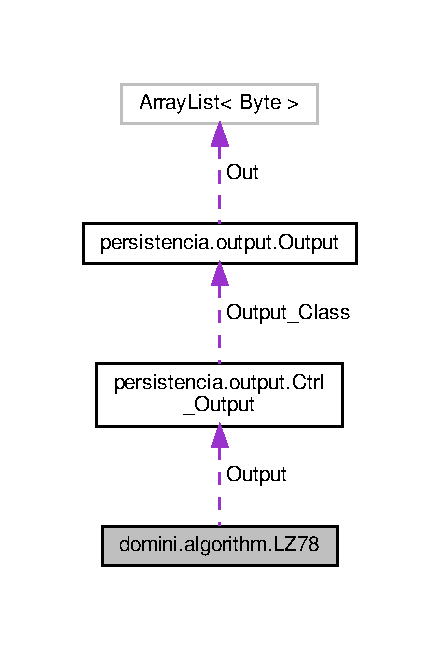
\includegraphics[width=211pt]{classdomini_1_1algorithm_1_1LZ78__coll__graph}
\end{center}
\end{figure}
\subsection*{Public Member Functions}
\begin{DoxyCompactItemize}
\item 
\hyperlink{classdomini_1_1algorithm_1_1LZ78_a89c121da8ae75e24f1cf0d06530d0b89}{L\+Z78} (String path, boolean b)
\begin{DoxyCompactList}\small\item\em Constructor de la classe. \end{DoxyCompactList}\item 
\hyperlink{classdomini_1_1algorithm_1_1LZ78_abdeba774404b53d266e9fbe4aa35f757}{L\+Z78} (boolean b)
\begin{DoxyCompactList}\small\item\em Constructor de la classe. \end{DoxyCompactList}\item 
void \hyperlink{classdomini_1_1algorithm_1_1LZ78_a6ce2ce6b2ce14cbe5177f379becbb2d1}{Compressor} ()
\begin{DoxyCompactList}\small\item\em Comprimim un text amb l\textquotesingle{}algoritme \hyperlink{classdomini_1_1algorithm_1_1LZ78}{L\+Z78}. \end{DoxyCompactList}\item 
void \hyperlink{classdomini_1_1algorithm_1_1LZ78_a0872cb8224ffd478b992490df06f6ecf}{Decompressor} ()
\begin{DoxyCompactList}\small\item\em Descomprimim un fitxer amb l\textquotesingle{}algoritme \hyperlink{classdomini_1_1algorithm_1_1LZ78}{L\+Z78}. \end{DoxyCompactList}\end{DoxyCompactItemize}
\subsection*{Additional Inherited Members}


\subsection{Detailed Description}
Compressió i descompressió pel mètode \hyperlink{classdomini_1_1algorithm_1_1LZ78}{L\+Z78}. 

\subsection{Constructor \& Destructor Documentation}
\mbox{\Hypertarget{classdomini_1_1algorithm_1_1LZ78_a89c121da8ae75e24f1cf0d06530d0b89}\label{classdomini_1_1algorithm_1_1LZ78_a89c121da8ae75e24f1cf0d06530d0b89}} 
\index{domini\+::algorithm\+::\+L\+Z78@{domini\+::algorithm\+::\+L\+Z78}!L\+Z78@{L\+Z78}}
\index{L\+Z78@{L\+Z78}!domini\+::algorithm\+::\+L\+Z78@{domini\+::algorithm\+::\+L\+Z78}}
\subsubsection{\texorpdfstring{L\+Z78()}{LZ78()}\hspace{0.1cm}{\footnotesize\ttfamily [1/2]}}
{\footnotesize\ttfamily domini.\+algorithm.\+L\+Z78.\+L\+Z78 (\begin{DoxyParamCaption}\item[{String}]{path,  }\item[{boolean}]{b }\end{DoxyParamCaption})\hspace{0.3cm}{\ttfamily [inline]}}



Constructor de la classe. 


\begin{DoxyParams}{Parameters}
{\em path} & Path de sortida \\
\hline
{\em b} & False si estas comprimint, True si estas descomprimint \\
\hline
\end{DoxyParams}

\begin{DoxyCode}
27                                         \{
28         super(path, b);
29         \textcolor{keywordflow}{if} (!b) \{
30             \hyperlink{classdomini_1_1algorithm_1_1Algorithm_a4de9955411c656325adc391ef570c082}{Output}.\hyperlink{classpersistencia_1_1output_1_1Ctrl__Output_ae6d6857910a023982900ddc857b891f0}{addMetadata}(\textcolor{stringliteral}{"lz78"});
31         \}
32     \}
\end{DoxyCode}
\mbox{\Hypertarget{classdomini_1_1algorithm_1_1LZ78_abdeba774404b53d266e9fbe4aa35f757}\label{classdomini_1_1algorithm_1_1LZ78_abdeba774404b53d266e9fbe4aa35f757}} 
\index{domini\+::algorithm\+::\+L\+Z78@{domini\+::algorithm\+::\+L\+Z78}!L\+Z78@{L\+Z78}}
\index{L\+Z78@{L\+Z78}!domini\+::algorithm\+::\+L\+Z78@{domini\+::algorithm\+::\+L\+Z78}}
\subsubsection{\texorpdfstring{L\+Z78()}{LZ78()}\hspace{0.1cm}{\footnotesize\ttfamily [2/2]}}
{\footnotesize\ttfamily domini.\+algorithm.\+L\+Z78.\+L\+Z78 (\begin{DoxyParamCaption}\item[{boolean}]{b }\end{DoxyParamCaption})\hspace{0.3cm}{\ttfamily [inline]}}



Constructor de la classe. 


\begin{DoxyParams}{Parameters}
{\em b} & False si estas comprimint, True si estas descomprimint \\
\hline
\end{DoxyParams}
\begin{DoxyNote}{Note}
Es continua escrivint al fitxer que s\textquotesingle{}estava escrivint 
\end{DoxyNote}

\begin{DoxyCode}
39                            \{
40         super(b);
41         \textcolor{keywordflow}{if} (!b) \{
42             \hyperlink{classdomini_1_1algorithm_1_1Algorithm_a4de9955411c656325adc391ef570c082}{Output}.\hyperlink{classpersistencia_1_1output_1_1Ctrl__Output_ae6d6857910a023982900ddc857b891f0}{addMetadata}(\textcolor{stringliteral}{"lz78"});
43         \}
44     \}
\end{DoxyCode}


\subsection{Member Function Documentation}
\mbox{\Hypertarget{classdomini_1_1algorithm_1_1LZ78_a6ce2ce6b2ce14cbe5177f379becbb2d1}\label{classdomini_1_1algorithm_1_1LZ78_a6ce2ce6b2ce14cbe5177f379becbb2d1}} 
\index{domini\+::algorithm\+::\+L\+Z78@{domini\+::algorithm\+::\+L\+Z78}!Compressor@{Compressor}}
\index{Compressor@{Compressor}!domini\+::algorithm\+::\+L\+Z78@{domini\+::algorithm\+::\+L\+Z78}}
\subsubsection{\texorpdfstring{Compressor()}{Compressor()}}
{\footnotesize\ttfamily public domini.\+algorithm.\+L\+Z78.\+Compressor (\begin{DoxyParamCaption}{ }\end{DoxyParamCaption})\hspace{0.3cm}{\ttfamily [inline]}}



Comprimim un text amb l\textquotesingle{}algoritme \hyperlink{classdomini_1_1algorithm_1_1LZ78}{L\+Z78}. 


\begin{DoxyCode}
51                              \{
52 
53         \hyperlink{classdomini_1_1algorithm_1_1Algorithm_a070b7e7dcc453b03751d265beae5306c}{checkCompressor}();
54         \hyperlink{classpersistencia_1_1input_1_1Ctrl__Input__Text}{Ctrl\_Input\_Text} in = \textcolor{keyword}{new} \hyperlink{classpersistencia_1_1input_1_1Ctrl__Input__Text}{Ctrl\_Input\_Text}();
55 
56         \hyperlink{classdomini_1_1utils_1_1Trie}{Trie<Byte>} map = \textcolor{keyword}{new} \hyperlink{classdomini_1_1utils_1_1Trie}{Trie<Byte>}();
57         Byte nextByte;  
58         ArrayList<Byte> seq = \textcolor{keyword}{new} ArrayList<Byte>();
59         Integer punterMap = 0;
60         \textcolor{keywordflow}{while}(!in.\hyperlink{classpersistencia_1_1input_1_1Ctrl__Input_a5a94d207dce0fd592b5ac17f55154d4f}{finished}()) \{
61             nextByte = in.\hyperlink{classpersistencia_1_1input_1_1Ctrl__Input__Text_a8b501ae723f8c6f8d63305a56e9720c3}{get}();
62             ArrayList<Byte> novaEntrada = \textcolor{keyword}{new} ArrayList<Byte> ();
63             novaEntrada.addAll(seq);
64             novaEntrada.add(nextByte);
65             \textcolor{keywordflow}{if}(map.\hyperlink{classdomini_1_1utils_1_1Trie_a5c30e36df9ab804bbc054805358ecf2a}{indexNode}(novaEntrada) != -1) \{
66                 \textcolor{keywordflow}{if}(in.\hyperlink{classpersistencia_1_1input_1_1Ctrl__Input_a5a94d207dce0fd592b5ac17f55154d4f}{finished}())\{
67                     Integer punterActual = map.\hyperlink{classdomini_1_1utils_1_1Trie_a5c30e36df9ab804bbc054805358ecf2a}{indexNode}(seq) +1;
68                     \hyperlink{classdomini_1_1algorithm_1_1Algorithm_a4de9955411c656325adc391ef570c082}{Output}.\hyperlink{classpersistencia_1_1output_1_1Ctrl__Output_a8c5aa5a6acb5259faeb1c05c71ddd21c}{add}((Integer)punterActual, 32);
69                     \hyperlink{classdomini_1_1algorithm_1_1Algorithm_a4de9955411c656325adc391ef570c082}{Output}.\hyperlink{classpersistencia_1_1output_1_1Ctrl__Output_a8c5aa5a6acb5259faeb1c05c71ddd21c}{add}(nextByte, 8);   
70                     \textcolor{keywordflow}{return};
71                 \}
72                 seq.add(nextByte);
73             \}\textcolor{keywordflow}{else}
74             \{                                   
75                 \textcolor{keywordflow}{if}(seq.size() >= 1)\{
76                     Integer punterActual = map.\hyperlink{classdomini_1_1utils_1_1Trie_a5c30e36df9ab804bbc054805358ecf2a}{indexNode}(seq) +1;
77                     
78                     \hyperlink{classdomini_1_1algorithm_1_1Algorithm_a4de9955411c656325adc391ef570c082}{Output}.\hyperlink{classpersistencia_1_1output_1_1Ctrl__Output_a8c5aa5a6acb5259faeb1c05c71ddd21c}{add}((Integer)punterActual, 32);
79 
80                 \}\textcolor{keywordflow}{else}\{
81                     \hyperlink{classdomini_1_1algorithm_1_1Algorithm_a4de9955411c656325adc391ef570c082}{Output}.\hyperlink{classpersistencia_1_1output_1_1Ctrl__Output_a8c5aa5a6acb5259faeb1c05c71ddd21c}{add}((Integer)0, 32);
82                 \}
83                 
84                 \hyperlink{classdomini_1_1algorithm_1_1Algorithm_a4de9955411c656325adc391ef570c082}{Output}.\hyperlink{classpersistencia_1_1output_1_1Ctrl__Output_a8c5aa5a6acb5259faeb1c05c71ddd21c}{add}(nextByte, 8);
85 
86                 map.\hyperlink{classdomini_1_1utils_1_1Trie_a3599001d9b056f0b54ab7eabb9d3510b}{insert}(novaEntrada, punterMap);
87 
88                 seq = \textcolor{keyword}{new} ArrayList<Byte>();
89                 punterMap++;
90             \}
91         \}
92     \}
\end{DoxyCode}
\mbox{\Hypertarget{classdomini_1_1algorithm_1_1LZ78_a0872cb8224ffd478b992490df06f6ecf}\label{classdomini_1_1algorithm_1_1LZ78_a0872cb8224ffd478b992490df06f6ecf}} 
\index{domini\+::algorithm\+::\+L\+Z78@{domini\+::algorithm\+::\+L\+Z78}!Decompressor@{Decompressor}}
\index{Decompressor@{Decompressor}!domini\+::algorithm\+::\+L\+Z78@{domini\+::algorithm\+::\+L\+Z78}}
\subsubsection{\texorpdfstring{Decompressor()}{Decompressor()}}
{\footnotesize\ttfamily public domini.\+algorithm.\+L\+Z78.\+Decompressor (\begin{DoxyParamCaption}{ }\end{DoxyParamCaption})\hspace{0.3cm}{\ttfamily [inline]}}



Descomprimim un fitxer amb l\textquotesingle{}algoritme \hyperlink{classdomini_1_1algorithm_1_1LZ78}{L\+Z78}. 


\begin{DoxyCode}
98                                \{
99 
100         \hyperlink{classdomini_1_1algorithm_1_1Algorithm_a6b738342cc7169893fa60d593f5a13db}{checkDecompressor}();
101         \hyperlink{classpersistencia_1_1input_1_1Ctrl__Input__LZ78}{Ctrl\_Input\_LZ78} in = \textcolor{keyword}{new} \hyperlink{classpersistencia_1_1input_1_1Ctrl__Input__LZ78}{Ctrl\_Input\_LZ78}();
102 
103         \hyperlink{classdomini_1_1utils_1_1Dict__Decode}{Dict\_Decode} map = \textcolor{keyword}{new} \hyperlink{classdomini_1_1utils_1_1Dict__Decode}{Dict\_Decode}(\textcolor{keyword}{false}, 0);
104         \textcolor{keywordflow}{while}(!in.\hyperlink{classpersistencia_1_1input_1_1Ctrl__Input_a5a94d207dce0fd592b5ac17f55154d4f}{finished}()) \{
105             \hyperlink{classdomini_1_1utils_1_1Pair}{Pair <Integer, Byte>} entr = in.\hyperlink{classpersistencia_1_1input_1_1Ctrl__Input__LZ78_ae09535962f284be3a76369845c15b78c}{get}();
106             \textcolor{keywordflow}{if}(in.\hyperlink{classpersistencia_1_1input_1_1Ctrl__Input_a5a94d207dce0fd592b5ac17f55154d4f}{finished}()) \textcolor{keywordflow}{return};
107             Integer punterMap = entr.\hyperlink{classdomini_1_1utils_1_1Pair_a9439fbd8488cb1fbf00c57f15f093c4b}{getLeft}();
108             Byte nextByte = entr.\hyperlink{classdomini_1_1utils_1_1Pair_a0dca94eb1a43952258bebe1dca4c84e9}{getRight}();
109 
110             ArrayList<Byte> seqPunterMap = map.\hyperlink{classdomini_1_1utils_1_1Dict__Decode_a0f6457460aefe9df50f0cad48f58feee}{getWord}(punterMap);
111             seqPunterMap.add(nextByte);
112             map.\hyperlink{classdomini_1_1utils_1_1Dict__Decode_a077011e4507db308d143ea9b7146abb9}{add}(punterMap, nextByte);
113             \hyperlink{classdomini_1_1algorithm_1_1Algorithm_a4de9955411c656325adc391ef570c082}{Output}.\hyperlink{classpersistencia_1_1output_1_1Ctrl__Output_a8c5aa5a6acb5259faeb1c05c71ddd21c}{add}(seqPunterMap);
114         \}
115     \}
\end{DoxyCode}


The documentation for this class was generated from the following file\+:\begin{DoxyCompactItemize}
\item 
src/domini/algorithm/\hyperlink{LZ78_8java}{L\+Z78.\+java}\end{DoxyCompactItemize}

\hypertarget{classdomini_1_1algorithm_1_1LZSS}{}\section{domini.\+algorithm.\+L\+Z\+SS Class Reference}
\label{classdomini_1_1algorithm_1_1LZSS}\index{domini.\+algorithm.\+L\+Z\+SS@{domini.\+algorithm.\+L\+Z\+SS}}


Aquesta és la classe del algoritme \hyperlink{classdomini_1_1algorithm_1_1LZSS}{L\+Z\+SS}.  


\subsection*{Public Member Functions}
\begin{DoxyCompactItemize}
\item 
\hyperlink{classdomini_1_1algorithm_1_1LZSS_a991f29ccc89ecbb5645ea8f123205e20}{L\+Z\+SS} (String aux, boolean b)
\begin{DoxyCompactList}\small\item\em El constructor. \end{DoxyCompactList}\item 
\hyperlink{classpersistencia_1_1output_1_1Ctrl__Output}{Ctrl\+\_\+\+Output} \hyperlink{classdomini_1_1algorithm_1_1LZSS_a8172ff7c8aefb87c90c648bc1b6b78b9}{print} ()
\begin{DoxyCompactList}\small\item\em Mètode print. \end{DoxyCompactList}\item 
void \hyperlink{classdomini_1_1algorithm_1_1LZSS_a385d06ea406b7a0f1168370e9574531a}{Compressor} (\hyperlink{classpersistencia_1_1input_1_1Ctrl__Input__Text}{Ctrl\+\_\+\+Input\+\_\+\+Text} in)
\begin{DoxyCompactList}\small\item\em Mètode principal per a la compressió. \end{DoxyCompactList}\item 
void \hyperlink{classdomini_1_1algorithm_1_1LZSS_a3fcf941d4301a4a857c585b3770a0ecf}{Decompressor} (\hyperlink{classpersistencia_1_1input_1_1Ctrl__Input__LZSS}{Ctrl\+\_\+\+Input\+\_\+\+L\+Z\+SS} in)
\begin{DoxyCompactList}\small\item\em Mètode principal per a la descompressió. \end{DoxyCompactList}\end{DoxyCompactItemize}


\subsection{Detailed Description}
Aquesta és la classe del algoritme \hyperlink{classdomini_1_1algorithm_1_1LZSS}{L\+Z\+SS}. 

En aquesta classe es tracta la compressió mitjançant l\textquotesingle{}algorisme \hyperlink{classdomini_1_1algorithm_1_1LZSS}{L\+Z\+SS} i la descompressió d\textquotesingle{}un input el qual ha estat comprimit amb aquest mateix algoritme.

\begin{DoxyAuthor}{Author}
Manel Aguilar 
\end{DoxyAuthor}


\subsection{Constructor \& Destructor Documentation}
\mbox{\Hypertarget{classdomini_1_1algorithm_1_1LZSS_a991f29ccc89ecbb5645ea8f123205e20}\label{classdomini_1_1algorithm_1_1LZSS_a991f29ccc89ecbb5645ea8f123205e20}} 
\index{domini\+::algorithm\+::\+L\+Z\+SS@{domini\+::algorithm\+::\+L\+Z\+SS}!L\+Z\+SS@{L\+Z\+SS}}
\index{L\+Z\+SS@{L\+Z\+SS}!domini\+::algorithm\+::\+L\+Z\+SS@{domini\+::algorithm\+::\+L\+Z\+SS}}
\subsubsection{\texorpdfstring{L\+Z\+S\+S()}{LZSS()}}
{\footnotesize\ttfamily domini.\+algorithm.\+L\+Z\+S\+S.\+L\+Z\+SS (\begin{DoxyParamCaption}\item[{String}]{aux,  }\item[{boolean}]{b }\end{DoxyParamCaption})\hspace{0.3cm}{\ttfamily [inline]}}



El constructor. 


\begin{DoxyParams}{Parameters}
{\em aux} & inicialitza una instància Ctrl\+\_\+\+Output. \\
\hline
{\em b} & Si false comprimeix else descomprimeix. \\
\hline
\end{DoxyParams}


\subsection{Member Function Documentation}
\mbox{\Hypertarget{classdomini_1_1algorithm_1_1LZSS_a385d06ea406b7a0f1168370e9574531a}\label{classdomini_1_1algorithm_1_1LZSS_a385d06ea406b7a0f1168370e9574531a}} 
\index{domini\+::algorithm\+::\+L\+Z\+SS@{domini\+::algorithm\+::\+L\+Z\+SS}!Compressor@{Compressor}}
\index{Compressor@{Compressor}!domini\+::algorithm\+::\+L\+Z\+SS@{domini\+::algorithm\+::\+L\+Z\+SS}}
\subsubsection{\texorpdfstring{Compressor()}{Compressor()}}
{\footnotesize\ttfamily public void domini.\+algorithm.\+L\+Z\+S\+S.\+Compressor (\begin{DoxyParamCaption}\item[{\hyperlink{classpersistencia_1_1input_1_1Ctrl__Input__Text}{Ctrl\+\_\+\+Input\+\_\+\+Text}}]{in }\end{DoxyParamCaption})\hspace{0.3cm}{\ttfamily [inline]}}



Mètode principal per a la compressió. 


\begin{DoxyParams}{Parameters}
{\em in} & És per anar agafant informació de la classe Ctrl\+\_\+\+Input\+\_\+\+Text. \\
\hline
\end{DoxyParams}
\mbox{\Hypertarget{classdomini_1_1algorithm_1_1LZSS_a3fcf941d4301a4a857c585b3770a0ecf}\label{classdomini_1_1algorithm_1_1LZSS_a3fcf941d4301a4a857c585b3770a0ecf}} 
\index{domini\+::algorithm\+::\+L\+Z\+SS@{domini\+::algorithm\+::\+L\+Z\+SS}!Decompressor@{Decompressor}}
\index{Decompressor@{Decompressor}!domini\+::algorithm\+::\+L\+Z\+SS@{domini\+::algorithm\+::\+L\+Z\+SS}}
\subsubsection{\texorpdfstring{Decompressor()}{Decompressor()}}
{\footnotesize\ttfamily public void domini.\+algorithm.\+L\+Z\+S\+S.\+Decompressor (\begin{DoxyParamCaption}\item[{\hyperlink{classpersistencia_1_1input_1_1Ctrl__Input__LZSS}{Ctrl\+\_\+\+Input\+\_\+\+L\+Z\+SS}}]{in }\end{DoxyParamCaption})\hspace{0.3cm}{\ttfamily [inline]}}



Mètode principal per a la descompressió. 


\begin{DoxyParams}{Parameters}
{\em in} & És per anar agafant informació de la classe Ctrl\+\_\+\+Input\+\_\+\+L\+Z\+SS. \\
\hline
\end{DoxyParams}
\mbox{\Hypertarget{classdomini_1_1algorithm_1_1LZSS_a8172ff7c8aefb87c90c648bc1b6b78b9}\label{classdomini_1_1algorithm_1_1LZSS_a8172ff7c8aefb87c90c648bc1b6b78b9}} 
\index{domini\+::algorithm\+::\+L\+Z\+SS@{domini\+::algorithm\+::\+L\+Z\+SS}!print@{print}}
\index{print@{print}!domini\+::algorithm\+::\+L\+Z\+SS@{domini\+::algorithm\+::\+L\+Z\+SS}}
\subsubsection{\texorpdfstring{print()}{print()}}
{\footnotesize\ttfamily public \hyperlink{classpersistencia_1_1output_1_1Ctrl__Output}{Ctrl\+\_\+\+Output} domini.\+algorithm.\+L\+Z\+S\+S.\+print (\begin{DoxyParamCaption}{ }\end{DoxyParamCaption})\hspace{0.3cm}{\ttfamily [inline]}}



Mètode print. 

\begin{DoxyReturn}{Returns}
Retorna l\textquotesingle{}atribut \char`\"{}\+Output\char`\"{}. 
\end{DoxyReturn}


The documentation for this class was generated from the following file\+:\begin{DoxyCompactItemize}
\item 
src/domini/algorithm/L\+Z\+S\+S.\+java\end{DoxyCompactItemize}

\hypertarget{classdomini_1_1algorithm_1_1LZW}{}\section{domini.\+algorithm.\+L\+ZW Class Reference}
\label{classdomini_1_1algorithm_1_1LZW}\index{domini.\+algorithm.\+L\+ZW@{domini.\+algorithm.\+L\+ZW}}


Compressió i descompressió pel mètode \hyperlink{classdomini_1_1algorithm_1_1LZW}{L\+ZW}.  




Collaboration diagram for domini.\+algorithm.\+L\+ZW\+:
\nopagebreak
\begin{figure}[H]
\begin{center}
\leavevmode
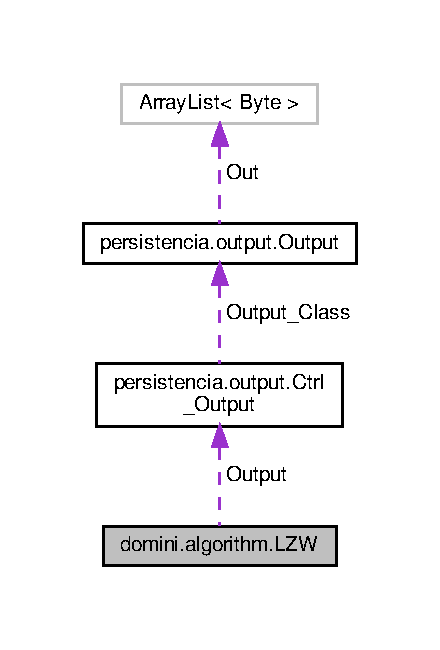
\includegraphics[width=211pt]{classdomini_1_1algorithm_1_1LZW__coll__graph}
\end{center}
\end{figure}
\subsection*{Public Member Functions}
\begin{DoxyCompactItemize}
\item 
\hyperlink{classdomini_1_1algorithm_1_1LZW_a00bd43f0691ac9679e6232b701e535ec}{L\+ZW} (String aux, boolean b)
\begin{DoxyCompactList}\small\item\em Constructor de la clase \hyperlink{classdomini_1_1algorithm_1_1LZW}{L\+ZW}. \end{DoxyCompactList}\item 
void \hyperlink{classdomini_1_1algorithm_1_1LZW_a79ce338289c3e8fcdd111ca029cfb45b}{compression} (\hyperlink{classpersistencia_1_1input_1_1Ctrl__Input__Text}{Ctrl\+\_\+\+Input\+\_\+\+Text} inp)
\begin{DoxyCompactList}\small\item\em Comprimim un text amb l\textquotesingle{}algoritme \hyperlink{classdomini_1_1algorithm_1_1LZW}{L\+ZW}. \end{DoxyCompactList}\item 
void \hyperlink{classdomini_1_1algorithm_1_1LZW_a1c7f66a62ed475a72a49f294c41f54fa}{decompression} (\hyperlink{classpersistencia_1_1input_1_1Ctrl__Input__LZW}{Ctrl\+\_\+\+Input\+\_\+\+L\+ZW} inp)
\begin{DoxyCompactList}\small\item\em Descomprimim un fitxer amb l\textquotesingle{}algoritme \hyperlink{classdomini_1_1algorithm_1_1LZW}{L\+ZW}. \end{DoxyCompactList}\item 
\hyperlink{classpersistencia_1_1output_1_1Ctrl__Output}{Ctrl\+\_\+\+Output} \hyperlink{classdomini_1_1algorithm_1_1LZW_a57ba5129e7f26d4cc066195e3d6c9c8c}{print} ()
\begin{DoxyCompactList}\small\item\em La funció serà cridada quan volguem obtenir el resultat d\textquotesingle{}una compressio o descompressio. \end{DoxyCompactList}\end{DoxyCompactItemize}


\subsection{Detailed Description}
Compressió i descompressió pel mètode \hyperlink{classdomini_1_1algorithm_1_1LZW}{L\+ZW}. 

\begin{DoxyAuthor}{Author}
Miguel Paracuellos Ocaña 
\end{DoxyAuthor}


\subsection{Constructor \& Destructor Documentation}
\mbox{\Hypertarget{classdomini_1_1algorithm_1_1LZW_a00bd43f0691ac9679e6232b701e535ec}\label{classdomini_1_1algorithm_1_1LZW_a00bd43f0691ac9679e6232b701e535ec}} 
\index{domini\+::algorithm\+::\+L\+ZW@{domini\+::algorithm\+::\+L\+ZW}!L\+ZW@{L\+ZW}}
\index{L\+ZW@{L\+ZW}!domini\+::algorithm\+::\+L\+ZW@{domini\+::algorithm\+::\+L\+ZW}}
\subsubsection{\texorpdfstring{L\+Z\+W()}{LZW()}}
{\footnotesize\ttfamily domini.\+algorithm.\+L\+Z\+W.\+L\+ZW (\begin{DoxyParamCaption}\item[{String}]{aux,  }\item[{boolean}]{b }\end{DoxyParamCaption})\hspace{0.3cm}{\ttfamily [inline]}}



Constructor de la clase \hyperlink{classdomini_1_1algorithm_1_1LZW}{L\+ZW}. 


\begin{DoxyParams}{Parameters}
{\em aux} & Path de sortida \\
\hline
\end{DoxyParams}


\subsection{Member Function Documentation}
\mbox{\Hypertarget{classdomini_1_1algorithm_1_1LZW_a79ce338289c3e8fcdd111ca029cfb45b}\label{classdomini_1_1algorithm_1_1LZW_a79ce338289c3e8fcdd111ca029cfb45b}} 
\index{domini\+::algorithm\+::\+L\+ZW@{domini\+::algorithm\+::\+L\+ZW}!compression@{compression}}
\index{compression@{compression}!domini\+::algorithm\+::\+L\+ZW@{domini\+::algorithm\+::\+L\+ZW}}
\subsubsection{\texorpdfstring{compression()}{compression()}}
{\footnotesize\ttfamily public Array\+List$<$ Integer $>$ domini.\+algorithm.\+L\+Z\+W.\+compression (\begin{DoxyParamCaption}\item[{\hyperlink{classpersistencia_1_1input_1_1Ctrl__Input__Text}{Ctrl\+\_\+\+Input\+\_\+\+Text}}]{inp }\end{DoxyParamCaption})\hspace{0.3cm}{\ttfamily [inline]}}



Comprimim un text amb l\textquotesingle{}algoritme \hyperlink{classdomini_1_1algorithm_1_1LZW}{L\+ZW}. 


\begin{DoxyParams}{Parameters}
{\em inp} & accés al Controlador d\textquotesingle{}Input per el text \\
\hline
\end{DoxyParams}
\begin{DoxyReturn}{Returns}
llista amb els enters que representen el text 
\end{DoxyReturn}
\mbox{\Hypertarget{classdomini_1_1algorithm_1_1LZW_a1c7f66a62ed475a72a49f294c41f54fa}\label{classdomini_1_1algorithm_1_1LZW_a1c7f66a62ed475a72a49f294c41f54fa}} 
\index{domini\+::algorithm\+::\+L\+ZW@{domini\+::algorithm\+::\+L\+ZW}!decompression@{decompression}}
\index{decompression@{decompression}!domini\+::algorithm\+::\+L\+ZW@{domini\+::algorithm\+::\+L\+ZW}}
\subsubsection{\texorpdfstring{decompression()}{decompression()}}
{\footnotesize\ttfamily public String domini.\+algorithm.\+L\+Z\+W.\+decompression (\begin{DoxyParamCaption}\item[{\hyperlink{classpersistencia_1_1input_1_1Ctrl__Input__LZW}{Ctrl\+\_\+\+Input\+\_\+\+L\+ZW}}]{inp }\end{DoxyParamCaption})\hspace{0.3cm}{\ttfamily [inline]}}



Descomprimim un fitxer amb l\textquotesingle{}algoritme \hyperlink{classdomini_1_1algorithm_1_1LZW}{L\+ZW}. 


\begin{DoxyParams}{Parameters}
{\em inp} & accés al Controlador d\textquotesingle{}Input pel fitxer comprimit \\
\hline
\end{DoxyParams}
\begin{DoxyReturn}{Returns}
text que representa el fitxer descomprimit 
\end{DoxyReturn}
\mbox{\Hypertarget{classdomini_1_1algorithm_1_1LZW_a57ba5129e7f26d4cc066195e3d6c9c8c}\label{classdomini_1_1algorithm_1_1LZW_a57ba5129e7f26d4cc066195e3d6c9c8c}} 
\index{domini\+::algorithm\+::\+L\+ZW@{domini\+::algorithm\+::\+L\+ZW}!print@{print}}
\index{print@{print}!domini\+::algorithm\+::\+L\+ZW@{domini\+::algorithm\+::\+L\+ZW}}
\subsubsection{\texorpdfstring{print()}{print()}}
{\footnotesize\ttfamily public \hyperlink{classpersistencia_1_1output_1_1Ctrl__Output}{Ctrl\+\_\+\+Output} domini.\+algorithm.\+L\+Z\+W.\+print (\begin{DoxyParamCaption}{ }\end{DoxyParamCaption})\hspace{0.3cm}{\ttfamily [inline]}}



La funció serà cridada quan volguem obtenir el resultat d\textquotesingle{}una compressio o descompressio. 

\begin{DoxyReturn}{Returns}
Controlador d\textquotesingle{}Output per poder esciure el resultat 
\end{DoxyReturn}


The documentation for this class was generated from the following file\+:\begin{DoxyCompactItemize}
\item 
src/domini/algorithm/L\+Z\+W.\+java\end{DoxyCompactItemize}

\hypertarget{classdomini_1_1algorithm_1_1LZWTest}{}\section{domini.\+algorithm.\+L\+Z\+W\+Test Class Reference}
\label{classdomini_1_1algorithm_1_1LZWTest}\index{domini.\+algorithm.\+L\+Z\+W\+Test@{domini.\+algorithm.\+L\+Z\+W\+Test}}


Junit de la classe \hyperlink{classdomini_1_1algorithm_1_1LZW}{L\+ZW}.  




Collaboration diagram for domini.\+algorithm.\+L\+Z\+W\+Test\+:
% FIG 0
\subsection*{Public Member Functions}
\begin{DoxyCompactItemize}
\item 
void \hyperlink{classdomini_1_1algorithm_1_1LZWTest_ae43f1a846dc9672b04c707314006a878}{test\+Compression} ()
\begin{DoxyCompactList}\small\item\em Comprovació del correcte funcionament de la compressio per \hyperlink{classdomini_1_1algorithm_1_1LZW}{L\+ZW}. \end{DoxyCompactList}\item 
void \hyperlink{classdomini_1_1algorithm_1_1LZWTest_aa9f013d2d8e008768c6c7b8fe319b534}{test\+Decompression} ()
\begin{DoxyCompactList}\small\item\em Comprovació del correcte funcionament de la descompressio per \hyperlink{classdomini_1_1algorithm_1_1LZW}{L\+ZW}. \end{DoxyCompactList}\end{DoxyCompactItemize}
\subsection*{Private Member Functions}
\begin{DoxyCompactItemize}
\item 
void \hyperlink{classdomini_1_1algorithm_1_1LZWTest_acf4cac88aafa2144dc8ce3a80453fa90}{initialize} (String path, boolean b)
\begin{DoxyCompactList}\small\item\em Inicialitza l\textquotesingle{}atribut lzw. \end{DoxyCompactList}\end{DoxyCompactItemize}
\subsection*{Private Attributes}
\begin{DoxyCompactItemize}
\item 
\hyperlink{classdomini_1_1algorithm_1_1LZW}{L\+ZW} \hyperlink{classdomini_1_1algorithm_1_1LZWTest_a591c1bb9b927631d0e60a2853e502d20}{lzw}
\item 
String \hyperlink{classdomini_1_1algorithm_1_1LZWTest_af5091e6df88845c585e92165f2fae2dc}{path\+\_\+lzw} = \char`\"{}../src/persistencia/data/junit/junit.\+jm\char`\"{}
\item 
String \hyperlink{classdomini_1_1algorithm_1_1LZWTest_a25a37b8cd7cb0756531c39e7ebc60db0}{path\+\_\+lzw\+\_\+check} = \char`\"{}../src/persistencia/data/junit/junit\+\_\+check.\+jm\char`\"{}
\item 
String \hyperlink{classdomini_1_1algorithm_1_1LZWTest_add9dbf2d86413bf9f7bcdd23b268c288}{path\+\_\+txt\+\_\+check} = \char`\"{}../src/persistencia/data/junit/junit\+\_\+check.\+txt\char`\"{}
\item 
String \hyperlink{classdomini_1_1algorithm_1_1LZWTest_a4194ade234060b69729a0380ff4ae33d}{path\+\_\+txt} = \char`\"{}../src/persistencia/data/junit/junit.\+txt\char`\"{}
\end{DoxyCompactItemize}


\subsection{Detailed Description}
Junit de la classe \hyperlink{classdomini_1_1algorithm_1_1LZW}{L\+ZW}. 

\begin{DoxyAuthor}{Author}
Miguel Paracuellos Ocaña 
\end{DoxyAuthor}


\subsection{Member Function Documentation}
\mbox{\Hypertarget{classdomini_1_1algorithm_1_1LZWTest_acf4cac88aafa2144dc8ce3a80453fa90}\label{classdomini_1_1algorithm_1_1LZWTest_acf4cac88aafa2144dc8ce3a80453fa90}} 
\index{domini\+::algorithm\+::\+L\+Z\+W\+Test@{domini\+::algorithm\+::\+L\+Z\+W\+Test}!initialize@{initialize}}
\index{initialize@{initialize}!domini\+::algorithm\+::\+L\+Z\+W\+Test@{domini\+::algorithm\+::\+L\+Z\+W\+Test}}
\subsubsection{\texorpdfstring{initialize()}{initialize()}}
{\footnotesize\ttfamily private void domini.\+algorithm.\+L\+Z\+W\+Test.\+initialize (\begin{DoxyParamCaption}\item[{String}]{path,  }\item[{boolean}]{b }\end{DoxyParamCaption})\hspace{0.3cm}{\ttfamily [inline]}, {\ttfamily [private]}}



Inicialitza l\textquotesingle{}atribut lzw. 


\begin{DoxyParams}{Parameters}
{\em path} & Primer paràmetre del constructor lzw \\
\hline
{\em b} & Segon paràmetre del constructor lzw \\
\hline
\end{DoxyParams}

\begin{DoxyCode}
35                                                     \{
36         \hyperlink{classdomini_1_1algorithm_1_1LZWTest_a591c1bb9b927631d0e60a2853e502d20}{lzw} = \textcolor{keyword}{new} LZW(path, b);
37     \}
\end{DoxyCode}
\mbox{\Hypertarget{classdomini_1_1algorithm_1_1LZWTest_ae43f1a846dc9672b04c707314006a878}\label{classdomini_1_1algorithm_1_1LZWTest_ae43f1a846dc9672b04c707314006a878}} 
\index{domini\+::algorithm\+::\+L\+Z\+W\+Test@{domini\+::algorithm\+::\+L\+Z\+W\+Test}!test\+Compression@{test\+Compression}}
\index{test\+Compression@{test\+Compression}!domini\+::algorithm\+::\+L\+Z\+W\+Test@{domini\+::algorithm\+::\+L\+Z\+W\+Test}}
\subsubsection{\texorpdfstring{test\+Compression()}{testCompression()}}
{\footnotesize\ttfamily public void domini.\+algorithm.\+L\+Z\+W\+Test.\+test\+Compression (\begin{DoxyParamCaption}{ }\end{DoxyParamCaption})\hspace{0.3cm}{\ttfamily [inline]}}



Comprovació del correcte funcionament de la compressio per \hyperlink{classdomini_1_1algorithm_1_1LZW}{L\+ZW}. 


\begin{DoxyCode}
44                                   \{
45         System.out.println(\textcolor{stringliteral}{"Comprovació de la compressio amb LZW: "});
46 
47         Ctrl\_Output aux = \textcolor{keyword}{new} Ctrl\_Output(\hyperlink{classdomini_1_1algorithm_1_1LZWTest_a25a37b8cd7cb0756531c39e7ebc60db0}{path\_lzw\_check});
48         aux.addMetadata(\textcolor{stringliteral}{"lzw"});
49         Integer[] compr = \{66,65,256,257,65,260\};
50         \textcolor{keywordflow}{for} (Integer x : compr) 
51             aux.add(x);
52         aux.print();
53 
54         \hyperlink{classdomini_1_1algorithm_1_1LZWTest_acf4cac88aafa2144dc8ce3a80453fa90}{initialize}(\hyperlink{classdomini_1_1algorithm_1_1LZWTest_af5091e6df88845c585e92165f2fae2dc}{path\_lzw}, \textcolor{keyword}{false});
55         Ctrl\_Input.initialize(\hyperlink{classdomini_1_1algorithm_1_1LZWTest_a4194ade234060b69729a0380ff4ae33d}{path\_txt});
56         \hyperlink{classdomini_1_1algorithm_1_1LZWTest_a591c1bb9b927631d0e60a2853e502d20}{lzw}.\hyperlink{classdomini_1_1algorithm_1_1LZW_a04a13292c78f6d958270fec8bc6975be}{Compressor}();
57         \hyperlink{classdomini_1_1algorithm_1_1LZWTest_a591c1bb9b927631d0e60a2853e502d20}{lzw}.\hyperlink{classdomini_1_1algorithm_1_1Algorithm_a5546f991f9d71d012d6ded5f2d4181cb}{print}();
58 
59         Ctrl\_Input\_LZW in = \textcolor{keyword}{new} Ctrl\_Input\_LZW(\hyperlink{classdomini_1_1algorithm_1_1LZWTest_af5091e6df88845c585e92165f2fae2dc}{path\_lzw});
60         ArrayList<Integer> arr1 = \textcolor{keyword}{new} ArrayList<>();
61         \textcolor{keywordflow}{while} (\textcolor{keyword}{true}) \{
62             Integer kk = in.get();
63             \textcolor{keywordflow}{if} (in.finished()) \textcolor{keywordflow}{break};
64             arr1.add(kk);
65         \}
66 
67         in = \textcolor{keyword}{new} Ctrl\_Input\_LZW(\hyperlink{classdomini_1_1algorithm_1_1LZWTest_af5091e6df88845c585e92165f2fae2dc}{path\_lzw});
68         ArrayList<Integer> arr2 = \textcolor{keyword}{new} ArrayList<>();
69         \textcolor{keywordflow}{while} (\textcolor{keyword}{true}) \{
70             Integer kk = in.get();
71             \textcolor{keywordflow}{if} (in.finished()) \textcolor{keywordflow}{break};
72             arr2.add(kk);
73         \}
74         
75         assertEquals(\textcolor{stringliteral}{"El contigut no és l'esperat"}, arr1.size(), arr2.size());
76         \textcolor{keywordflow}{for} (\textcolor{keywordtype}{int} i = 0; i < arr1.size(); ++i) \{
77             assertEquals(\textcolor{stringliteral}{"El contigut no és l'esperat"},arr1.get(i), arr2.get(i));
78         \}
79 
80         System.out.println(\textcolor{stringliteral}{"Ok."});
81 
82     \}
\end{DoxyCode}
\mbox{\Hypertarget{classdomini_1_1algorithm_1_1LZWTest_aa9f013d2d8e008768c6c7b8fe319b534}\label{classdomini_1_1algorithm_1_1LZWTest_aa9f013d2d8e008768c6c7b8fe319b534}} 
\index{domini\+::algorithm\+::\+L\+Z\+W\+Test@{domini\+::algorithm\+::\+L\+Z\+W\+Test}!test\+Decompression@{test\+Decompression}}
\index{test\+Decompression@{test\+Decompression}!domini\+::algorithm\+::\+L\+Z\+W\+Test@{domini\+::algorithm\+::\+L\+Z\+W\+Test}}
\subsubsection{\texorpdfstring{test\+Decompression()}{testDecompression()}}
{\footnotesize\ttfamily public void domini.\+algorithm.\+L\+Z\+W\+Test.\+test\+Decompression (\begin{DoxyParamCaption}{ }\end{DoxyParamCaption})\hspace{0.3cm}{\ttfamily [inline]}}



Comprovació del correcte funcionament de la descompressio per \hyperlink{classdomini_1_1algorithm_1_1LZW}{L\+ZW}. 


\begin{DoxyCode}
89                                     \{
90         System.out.println(\textcolor{stringliteral}{"Comprovació de la descompressio amb LZW: "});
91         
92         Ctrl\_Output aux = \textcolor{keyword}{new} Ctrl\_Output(\hyperlink{classdomini_1_1algorithm_1_1LZWTest_add9dbf2d86413bf9f7bcdd23b268c288}{path\_txt\_check});
93         byte[] decomp = \{66,65,66,65,65,66,65,65,65\};
94         \textcolor{keywordflow}{for} (byte x : decomp) 
95             aux.add(x,8);
96         aux.print();
97         
98         \hyperlink{classdomini_1_1algorithm_1_1LZWTest_acf4cac88aafa2144dc8ce3a80453fa90}{initialize}(\hyperlink{classdomini_1_1algorithm_1_1LZWTest_a4194ade234060b69729a0380ff4ae33d}{path\_txt}, \textcolor{keyword}{true});
99 
100         \textcolor{keyword}{new} Ctrl\_Input\_LZW(\hyperlink{classdomini_1_1algorithm_1_1LZWTest_af5091e6df88845c585e92165f2fae2dc}{path\_lzw});
101         \hyperlink{classdomini_1_1algorithm_1_1LZWTest_a591c1bb9b927631d0e60a2853e502d20}{lzw}.\hyperlink{classdomini_1_1algorithm_1_1LZW_a6a5d986396443691861ac9ba41b2dd33}{Decompressor}();
102         \hyperlink{classdomini_1_1algorithm_1_1LZWTest_a591c1bb9b927631d0e60a2853e502d20}{lzw}.\hyperlink{classdomini_1_1algorithm_1_1Algorithm_a5546f991f9d71d012d6ded5f2d4181cb}{print}();
103 
104         Ctrl\_Input\_Text in = \textcolor{keyword}{new} Ctrl\_Input\_Text(\hyperlink{classdomini_1_1algorithm_1_1LZWTest_a4194ade234060b69729a0380ff4ae33d}{path\_txt});
105         ArrayList<Byte> arr1 = \textcolor{keyword}{new} ArrayList<>();
106         \textcolor{keywordflow}{while} (\textcolor{keyword}{true}) \{
107             Byte kk = in.get();
108             \textcolor{keywordflow}{if} (in.finished()) \textcolor{keywordflow}{break};
109             arr1.add(kk);
110         \}
111 
112         in = \textcolor{keyword}{new} Ctrl\_Input\_Text(\hyperlink{classdomini_1_1algorithm_1_1LZWTest_add9dbf2d86413bf9f7bcdd23b268c288}{path\_txt\_check});
113         ArrayList<Byte> arr2 = \textcolor{keyword}{new} ArrayList<>();
114         \textcolor{keywordflow}{while} (\textcolor{keyword}{true}) \{
115             Byte kk = in.get();
116             \textcolor{keywordflow}{if} (in.finished()) \textcolor{keywordflow}{break};
117             arr2.add(kk);
118         \}
119         
120         assertEquals(\textcolor{stringliteral}{"El contigut no és l'esperat"}, arr1.size(), arr2.size());
121         \textcolor{keywordflow}{for} (\textcolor{keywordtype}{int} i = 0; i < arr1.size(); ++i) \{
122             assertEquals(\textcolor{stringliteral}{"El contigut no és l'esperat"},arr1.get(i), arr2.get(i));
123         \}
124         System.out.println(\textcolor{stringliteral}{"Ok."});
125     \}
\end{DoxyCode}


\subsection{Member Data Documentation}
\mbox{\Hypertarget{classdomini_1_1algorithm_1_1LZWTest_a591c1bb9b927631d0e60a2853e502d20}\label{classdomini_1_1algorithm_1_1LZWTest_a591c1bb9b927631d0e60a2853e502d20}} 
\index{domini\+::algorithm\+::\+L\+Z\+W\+Test@{domini\+::algorithm\+::\+L\+Z\+W\+Test}!lzw@{lzw}}
\index{lzw@{lzw}!domini\+::algorithm\+::\+L\+Z\+W\+Test@{domini\+::algorithm\+::\+L\+Z\+W\+Test}}
\subsubsection{\texorpdfstring{lzw}{lzw}}
{\footnotesize\ttfamily \hyperlink{classdomini_1_1algorithm_1_1LZW}{L\+ZW} domini.\+algorithm.\+L\+Z\+W\+Test.\+lzw\hspace{0.3cm}{\ttfamily [private]}}


\begin{DoxyParams}{Parameters}
{\em lzw} & Atribut de tipu \hyperlink{classdomini_1_1algorithm_1_1LZW}{L\+ZW} per a la comprovació de la classe \\
\hline
\end{DoxyParams}
\mbox{\Hypertarget{classdomini_1_1algorithm_1_1LZWTest_af5091e6df88845c585e92165f2fae2dc}\label{classdomini_1_1algorithm_1_1LZWTest_af5091e6df88845c585e92165f2fae2dc}} 
\index{domini\+::algorithm\+::\+L\+Z\+W\+Test@{domini\+::algorithm\+::\+L\+Z\+W\+Test}!path\+\_\+lzw@{path\+\_\+lzw}}
\index{path\+\_\+lzw@{path\+\_\+lzw}!domini\+::algorithm\+::\+L\+Z\+W\+Test@{domini\+::algorithm\+::\+L\+Z\+W\+Test}}
\subsubsection{\texorpdfstring{path\+\_\+lzw}{path\_lzw}}
{\footnotesize\ttfamily String domini.\+algorithm.\+L\+Z\+W\+Test.\+path\+\_\+lzw = \char`\"{}../src/persistencia/data/junit/junit.\+jm\char`\"{}\hspace{0.3cm}{\ttfamily [private]}}

\mbox{\Hypertarget{classdomini_1_1algorithm_1_1LZWTest_a25a37b8cd7cb0756531c39e7ebc60db0}\label{classdomini_1_1algorithm_1_1LZWTest_a25a37b8cd7cb0756531c39e7ebc60db0}} 
\index{domini\+::algorithm\+::\+L\+Z\+W\+Test@{domini\+::algorithm\+::\+L\+Z\+W\+Test}!path\+\_\+lzw\+\_\+check@{path\+\_\+lzw\+\_\+check}}
\index{path\+\_\+lzw\+\_\+check@{path\+\_\+lzw\+\_\+check}!domini\+::algorithm\+::\+L\+Z\+W\+Test@{domini\+::algorithm\+::\+L\+Z\+W\+Test}}
\subsubsection{\texorpdfstring{path\+\_\+lzw\+\_\+check}{path\_lzw\_check}}
{\footnotesize\ttfamily String domini.\+algorithm.\+L\+Z\+W\+Test.\+path\+\_\+lzw\+\_\+check = \char`\"{}../src/persistencia/data/junit/junit\+\_\+check.\+jm\char`\"{}\hspace{0.3cm}{\ttfamily [private]}}

\mbox{\Hypertarget{classdomini_1_1algorithm_1_1LZWTest_a4194ade234060b69729a0380ff4ae33d}\label{classdomini_1_1algorithm_1_1LZWTest_a4194ade234060b69729a0380ff4ae33d}} 
\index{domini\+::algorithm\+::\+L\+Z\+W\+Test@{domini\+::algorithm\+::\+L\+Z\+W\+Test}!path\+\_\+txt@{path\+\_\+txt}}
\index{path\+\_\+txt@{path\+\_\+txt}!domini\+::algorithm\+::\+L\+Z\+W\+Test@{domini\+::algorithm\+::\+L\+Z\+W\+Test}}
\subsubsection{\texorpdfstring{path\+\_\+txt}{path\_txt}}
{\footnotesize\ttfamily String domini.\+algorithm.\+L\+Z\+W\+Test.\+path\+\_\+txt = \char`\"{}../src/persistencia/data/junit/junit.\+txt\char`\"{}\hspace{0.3cm}{\ttfamily [private]}}

\mbox{\Hypertarget{classdomini_1_1algorithm_1_1LZWTest_add9dbf2d86413bf9f7bcdd23b268c288}\label{classdomini_1_1algorithm_1_1LZWTest_add9dbf2d86413bf9f7bcdd23b268c288}} 
\index{domini\+::algorithm\+::\+L\+Z\+W\+Test@{domini\+::algorithm\+::\+L\+Z\+W\+Test}!path\+\_\+txt\+\_\+check@{path\+\_\+txt\+\_\+check}}
\index{path\+\_\+txt\+\_\+check@{path\+\_\+txt\+\_\+check}!domini\+::algorithm\+::\+L\+Z\+W\+Test@{domini\+::algorithm\+::\+L\+Z\+W\+Test}}
\subsubsection{\texorpdfstring{path\+\_\+txt\+\_\+check}{path\_txt\_check}}
{\footnotesize\ttfamily String domini.\+algorithm.\+L\+Z\+W\+Test.\+path\+\_\+txt\+\_\+check = \char`\"{}../src/persistencia/data/junit/junit\+\_\+check.\+txt\char`\"{}\hspace{0.3cm}{\ttfamily [private]}}



The documentation for this class was generated from the following file\+:\begin{DoxyCompactItemize}
\item 
src/domini/algorithm/\hyperlink{LZWTest_8java}{L\+Z\+W\+Test.\+java}\end{DoxyCompactItemize}

\hypertarget{classMain}{}\section{Main Class Reference}
\label{classMain}\index{Main@{Main}}


Classe \hyperlink{classMain}{Main}.  


\subsection*{Static Public Member Functions}
\begin{DoxyCompactItemize}
\item 
static void \hyperlink{classMain_a8a5d0f827edddff706cc0e6740d0579a}{main} (String\mbox{[}$\,$\mbox{]} args)
\begin{DoxyCompactList}\small\item\em \hyperlink{classMain}{Main} de la classe. \end{DoxyCompactList}\end{DoxyCompactItemize}


\subsection{Detailed Description}
Classe \hyperlink{classMain}{Main}. 

\begin{DoxyAuthor}{Author}
Joan Lapeyra 
\end{DoxyAuthor}


\subsection{Member Function Documentation}
\mbox{\Hypertarget{classMain_a8a5d0f827edddff706cc0e6740d0579a}\label{classMain_a8a5d0f827edddff706cc0e6740d0579a}} 
\index{Main@{Main}!main@{main}}
\index{main@{main}!Main@{Main}}
\subsubsection{\texorpdfstring{main()}{main()}}
{\footnotesize\ttfamily static void Main.\+main (\begin{DoxyParamCaption}\item[{String \mbox{[}$\,$\mbox{]}}]{args }\end{DoxyParamCaption})\hspace{0.3cm}{\ttfamily [inline]}, {\ttfamily [static]}}



\hyperlink{classMain}{Main} de la classe. 


\begin{DoxyParams}{Parameters}
{\em args} & \\
\hline
\end{DoxyParams}


The documentation for this class was generated from the following file\+:\begin{DoxyCompactItemize}
\item 
src/\hyperlink{Main_8java}{Main.\+java}\end{DoxyCompactItemize}

\hypertarget{classdomini_1_1utils_1_1Node}{}\section{domini.\+utils.\+Node Class Reference}
\label{classdomini_1_1utils_1_1Node}\index{domini.\+utils.\+Node@{domini.\+utils.\+Node}}


Representa un node emprat per la representació de cadenes de caràcters.  


\subsection*{Public Member Functions}
\begin{DoxyCompactItemize}
\item 
\hyperlink{classdomini_1_1utils_1_1Node_ae337ba617322158f0ac240c900350278}{Node} (byte \hyperlink{classdomini_1_1utils_1_1Node_a2fbef2557db813ae02a2d52032eaa6e1}{c})
\begin{DoxyCompactList}\small\item\em Constructor de la classe. \end{DoxyCompactList}\item 
void \hyperlink{classdomini_1_1utils_1_1Node_a5a1cbd1e7f1fd78b42050f563520a709}{Modify\+\_\+\+Left} (Integer i)
\begin{DoxyCompactList}\small\item\em Modifica el valor del fill esquerra. \end{DoxyCompactList}\item 
void \hyperlink{classdomini_1_1utils_1_1Node_a58d22f8330339b6d807cdef44d0eddf6}{Modify\+\_\+\+Right} (Integer i)
\begin{DoxyCompactList}\small\item\em Modifica el valor del fill dret. \end{DoxyCompactList}\item 
void \hyperlink{classdomini_1_1utils_1_1Node_a3fe2e958308c90d24607a4e191680089}{Modify\+\_\+\+First} (Integer i)
\begin{DoxyCompactList}\small\item\em Modifica el valor del primer acces. \end{DoxyCompactList}\end{DoxyCompactItemize}
\subsection*{Package Attributes}
\begin{DoxyCompactItemize}
\item 
Integer \hyperlink{classdomini_1_1utils_1_1Node_a42db9f259f129c72cab2052a0f8ba42a}{First}
\item 
byte \hyperlink{classdomini_1_1utils_1_1Node_a2fbef2557db813ae02a2d52032eaa6e1}{c}
\item 
Integer \hyperlink{classdomini_1_1utils_1_1Node_a2f1d911cf52953b29d42e5e020b82dbf}{Left}
\item 
Integer \hyperlink{classdomini_1_1utils_1_1Node_a73c97e595bad2513ee0a06ee4620236a}{Right}
\end{DoxyCompactItemize}


\subsection{Detailed Description}
Representa un node emprat per la representació de cadenes de caràcters. 

\begin{DoxyAuthor}{Author}
Miguel Paracuellos Ocaña 
\end{DoxyAuthor}


\subsection{Constructor \& Destructor Documentation}
\mbox{\Hypertarget{classdomini_1_1utils_1_1Node_ae337ba617322158f0ac240c900350278}\label{classdomini_1_1utils_1_1Node_ae337ba617322158f0ac240c900350278}} 
\index{domini\+::utils\+::\+Node@{domini\+::utils\+::\+Node}!Node@{Node}}
\index{Node@{Node}!domini\+::utils\+::\+Node@{domini\+::utils\+::\+Node}}
\subsubsection{\texorpdfstring{Node()}{Node()}}
{\footnotesize\ttfamily domini.\+utils.\+Node.\+Node (\begin{DoxyParamCaption}\item[{byte}]{c }\end{DoxyParamCaption})\hspace{0.3cm}{\ttfamily [inline]}}



Constructor de la classe. 


\begin{DoxyParams}{Parameters}
{\em c} & Valor del node \\
\hline
\end{DoxyParams}

\begin{DoxyCode}
36                         \{
37         \hyperlink{classdomini_1_1utils_1_1Node_a42db9f259f129c72cab2052a0f8ba42a}{First} = \hyperlink{classdomini_1_1utils_1_1Node_a2f1d911cf52953b29d42e5e020b82dbf}{Left} = \hyperlink{classdomini_1_1utils_1_1Node_a73c97e595bad2513ee0a06ee4620236a}{Right} = -1;
38         this.\hyperlink{classdomini_1_1utils_1_1Node_a2fbef2557db813ae02a2d52032eaa6e1}{c} = \hyperlink{classdomini_1_1utils_1_1Node_a2fbef2557db813ae02a2d52032eaa6e1}{c};
39     \}
\end{DoxyCode}


\subsection{Member Function Documentation}
\mbox{\Hypertarget{classdomini_1_1utils_1_1Node_a3fe2e958308c90d24607a4e191680089}\label{classdomini_1_1utils_1_1Node_a3fe2e958308c90d24607a4e191680089}} 
\index{domini\+::utils\+::\+Node@{domini\+::utils\+::\+Node}!Modify\+\_\+\+First@{Modify\+\_\+\+First}}
\index{Modify\+\_\+\+First@{Modify\+\_\+\+First}!domini\+::utils\+::\+Node@{domini\+::utils\+::\+Node}}
\subsubsection{\texorpdfstring{Modify\+\_\+\+First()}{Modify\_First()}}
{\footnotesize\ttfamily public void domini.\+utils.\+Node.\+Modify\+\_\+\+First (\begin{DoxyParamCaption}\item[{Integer}]{i }\end{DoxyParamCaption})\hspace{0.3cm}{\ttfamily [inline]}}



Modifica el valor del primer acces. 


\begin{DoxyParams}{Parameters}
{\em i} & Nou valor pel primer acces al node \\
\hline
\end{DoxyParams}

\begin{DoxyCode}
66                                         \{
67         this.\hyperlink{classdomini_1_1utils_1_1Node_a42db9f259f129c72cab2052a0f8ba42a}{First} = i;
68     \}
\end{DoxyCode}
\mbox{\Hypertarget{classdomini_1_1utils_1_1Node_a5a1cbd1e7f1fd78b42050f563520a709}\label{classdomini_1_1utils_1_1Node_a5a1cbd1e7f1fd78b42050f563520a709}} 
\index{domini\+::utils\+::\+Node@{domini\+::utils\+::\+Node}!Modify\+\_\+\+Left@{Modify\+\_\+\+Left}}
\index{Modify\+\_\+\+Left@{Modify\+\_\+\+Left}!domini\+::utils\+::\+Node@{domini\+::utils\+::\+Node}}
\subsubsection{\texorpdfstring{Modify\+\_\+\+Left()}{Modify\_Left()}}
{\footnotesize\ttfamily public void domini.\+utils.\+Node.\+Modify\+\_\+\+Left (\begin{DoxyParamCaption}\item[{Integer}]{i }\end{DoxyParamCaption})\hspace{0.3cm}{\ttfamily [inline]}}



Modifica el valor del fill esquerra. 


\begin{DoxyParams}{Parameters}
{\em i} & Nou valor pel fill esquerra \\
\hline
\end{DoxyParams}

\begin{DoxyCode}
48                                        \{
49         this.\hyperlink{classdomini_1_1utils_1_1Node_a2f1d911cf52953b29d42e5e020b82dbf}{Left} = i;
50     \}
\end{DoxyCode}
\mbox{\Hypertarget{classdomini_1_1utils_1_1Node_a58d22f8330339b6d807cdef44d0eddf6}\label{classdomini_1_1utils_1_1Node_a58d22f8330339b6d807cdef44d0eddf6}} 
\index{domini\+::utils\+::\+Node@{domini\+::utils\+::\+Node}!Modify\+\_\+\+Right@{Modify\+\_\+\+Right}}
\index{Modify\+\_\+\+Right@{Modify\+\_\+\+Right}!domini\+::utils\+::\+Node@{domini\+::utils\+::\+Node}}
\subsubsection{\texorpdfstring{Modify\+\_\+\+Right()}{Modify\_Right()}}
{\footnotesize\ttfamily public void domini.\+utils.\+Node.\+Modify\+\_\+\+Right (\begin{DoxyParamCaption}\item[{Integer}]{i }\end{DoxyParamCaption})\hspace{0.3cm}{\ttfamily [inline]}}



Modifica el valor del fill dret. 


\begin{DoxyParams}{Parameters}
{\em i} & Nou valor pel fill dret \\
\hline
\end{DoxyParams}

\begin{DoxyCode}
57                                         \{
58         this.\hyperlink{classdomini_1_1utils_1_1Node_a73c97e595bad2513ee0a06ee4620236a}{Right} = i;
59     \}
\end{DoxyCode}


\subsection{Member Data Documentation}
\mbox{\Hypertarget{classdomini_1_1utils_1_1Node_a2fbef2557db813ae02a2d52032eaa6e1}\label{classdomini_1_1utils_1_1Node_a2fbef2557db813ae02a2d52032eaa6e1}} 
\index{domini\+::utils\+::\+Node@{domini\+::utils\+::\+Node}!c@{c}}
\index{c@{c}!domini\+::utils\+::\+Node@{domini\+::utils\+::\+Node}}
\subsubsection{\texorpdfstring{c}{c}}
{\footnotesize\ttfamily byte domini.\+utils.\+Node.\+c\hspace{0.3cm}{\ttfamily [package]}}


\begin{DoxyParams}{Parameters}
{\em c} & Valor del node \\
\hline
\end{DoxyParams}
\mbox{\Hypertarget{classdomini_1_1utils_1_1Node_a42db9f259f129c72cab2052a0f8ba42a}\label{classdomini_1_1utils_1_1Node_a42db9f259f129c72cab2052a0f8ba42a}} 
\index{domini\+::utils\+::\+Node@{domini\+::utils\+::\+Node}!First@{First}}
\index{First@{First}!domini\+::utils\+::\+Node@{domini\+::utils\+::\+Node}}
\subsubsection{\texorpdfstring{First}{First}}
{\footnotesize\ttfamily Integer domini.\+utils.\+Node.\+First\hspace{0.3cm}{\ttfamily [package]}}


\begin{DoxyParams}{Parameters}
{\em First} & Primer valor que accedeix a la seqüencia de caracters representada per aquest node \\
\hline
\end{DoxyParams}
\mbox{\Hypertarget{classdomini_1_1utils_1_1Node_a2f1d911cf52953b29d42e5e020b82dbf}\label{classdomini_1_1utils_1_1Node_a2f1d911cf52953b29d42e5e020b82dbf}} 
\index{domini\+::utils\+::\+Node@{domini\+::utils\+::\+Node}!Left@{Left}}
\index{Left@{Left}!domini\+::utils\+::\+Node@{domini\+::utils\+::\+Node}}
\subsubsection{\texorpdfstring{Left}{Left}}
{\footnotesize\ttfamily Integer domini.\+utils.\+Node.\+Left\hspace{0.3cm}{\ttfamily [package]}}


\begin{DoxyParams}{Parameters}
{\em Left} & fill esquerra \\
\hline
\end{DoxyParams}
\mbox{\Hypertarget{classdomini_1_1utils_1_1Node_a73c97e595bad2513ee0a06ee4620236a}\label{classdomini_1_1utils_1_1Node_a73c97e595bad2513ee0a06ee4620236a}} 
\index{domini\+::utils\+::\+Node@{domini\+::utils\+::\+Node}!Right@{Right}}
\index{Right@{Right}!domini\+::utils\+::\+Node@{domini\+::utils\+::\+Node}}
\subsubsection{\texorpdfstring{Right}{Right}}
{\footnotesize\ttfamily Integer domini.\+utils.\+Node.\+Right\hspace{0.3cm}{\ttfamily [package]}}


\begin{DoxyParams}{Parameters}
{\em Right} & fill dret \\
\hline
\end{DoxyParams}


The documentation for this class was generated from the following file\+:\begin{DoxyCompactItemize}
\item 
src/domini/utils/\hyperlink{Node_8java}{Node.\+java}\end{DoxyCompactItemize}

\hypertarget{classpersistencia_1_1output_1_1Output}{}\section{persistencia.\+output.\+Output Class Reference}
\label{classpersistencia_1_1output_1_1Output}\index{persistencia.\+output.\+Output@{persistencia.\+output.\+Output}}


Classe \hyperlink{classpersistencia_1_1output_1_1Output}{Output}.  




Collaboration diagram for persistencia.\+output.\+Output\+:\nopagebreak
\begin{figure}[H]
\begin{center}
\leavevmode
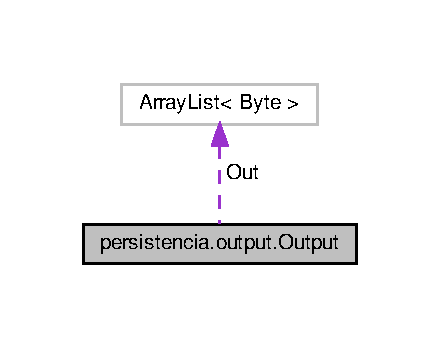
\includegraphics[width=211pt]{classpersistencia_1_1output_1_1Output__coll__graph}
\end{center}
\end{figure}
\subsection*{Public Member Functions}
\begin{DoxyCompactItemize}
\item 
\hyperlink{classpersistencia_1_1output_1_1Output_acbb70ea9eabb2a6d0b2d7bd2f3c9009a}{Output} (String \hyperlink{classpersistencia_1_1output_1_1Output_aebef717882f3bcc7080dec014c6714c9}{path})
\begin{DoxyCompactList}\small\item\em Constructor de la classe. \end{DoxyCompactList}\item 
void \hyperlink{classpersistencia_1_1output_1_1Output_adc03a0dd7a94da21fe8432064a4eec09}{add} (byte b, int n\+\_\+bits)
\begin{DoxyCompactList}\small\item\em Afegeix un byte amb n\+\_\+bits valids. \end{DoxyCompactList}\item 
\mbox{\Hypertarget{classpersistencia_1_1output_1_1Output_a416850e57f55bd371d60b2aae8e7e983}\label{classpersistencia_1_1output_1_1Output_a416850e57f55bd371d60b2aae8e7e983}} 
void {\bfseries print} ()
\item 
\mbox{\Hypertarget{classpersistencia_1_1output_1_1Output_ae6398e0602d281fd044d6557a16eb727}\label{classpersistencia_1_1output_1_1Output_ae6398e0602d281fd044d6557a16eb727}} 
void {\bfseries print\+String} ()
\item 
Array\+List$<$ Byte $>$ \hyperlink{classpersistencia_1_1output_1_1Output_ae4f870c86bed5b445125df989b313b9f}{get\+Out} ()
\item 
Integer \hyperlink{classpersistencia_1_1output_1_1Output_a01f862217e01efb59bc2eff3fe54006f}{get\+Pos} ()
\item 
String \hyperlink{classpersistencia_1_1output_1_1Output_ae33fc52334f791b6d4d7aebf2931df8d}{get\+Path} ()
\end{DoxyCompactItemize}
\subsection*{Package Attributes}
\begin{DoxyCompactItemize}
\item 
Array\+List$<$ Byte $>$ \hyperlink{classpersistencia_1_1output_1_1Output_ab993115d43930b7fb69e5d1c99addfba}{Out}
\item 
Integer \hyperlink{classpersistencia_1_1output_1_1Output_a3709182600423f7e57644ccdd0016f22}{Pos}
\item 
String \hyperlink{classpersistencia_1_1output_1_1Output_aebef717882f3bcc7080dec014c6714c9}{path}
\end{DoxyCompactItemize}


\subsection{Detailed Description}
Classe \hyperlink{classpersistencia_1_1output_1_1Output}{Output}. 

\begin{DoxyAuthor}{Author}
Manel Aguilar 
\end{DoxyAuthor}


\subsection{Constructor \& Destructor Documentation}
\mbox{\Hypertarget{classpersistencia_1_1output_1_1Output_acbb70ea9eabb2a6d0b2d7bd2f3c9009a}\label{classpersistencia_1_1output_1_1Output_acbb70ea9eabb2a6d0b2d7bd2f3c9009a}} 
\index{persistencia\+::output\+::\+Output@{persistencia\+::output\+::\+Output}!Output@{Output}}
\index{Output@{Output}!persistencia\+::output\+::\+Output@{persistencia\+::output\+::\+Output}}
\subsubsection{\texorpdfstring{Output()}{Output()}}
{\footnotesize\ttfamily persistencia.\+output.\+Output.\+Output (\begin{DoxyParamCaption}\item[{String}]{path }\end{DoxyParamCaption})\hspace{0.3cm}{\ttfamily [inline]}}



Constructor de la classe. 


\begin{DoxyParams}{Parameters}
{\em path} & Path de sortida \\
\hline
\end{DoxyParams}


\subsection{Member Function Documentation}
\mbox{\Hypertarget{classpersistencia_1_1output_1_1Output_adc03a0dd7a94da21fe8432064a4eec09}\label{classpersistencia_1_1output_1_1Output_adc03a0dd7a94da21fe8432064a4eec09}} 
\index{persistencia\+::output\+::\+Output@{persistencia\+::output\+::\+Output}!add@{add}}
\index{add@{add}!persistencia\+::output\+::\+Output@{persistencia\+::output\+::\+Output}}
\subsubsection{\texorpdfstring{add()}{add()}}
{\footnotesize\ttfamily public void persistencia.\+output.\+Output.\+add (\begin{DoxyParamCaption}\item[{byte}]{b,  }\item[{int}]{n\+\_\+bits }\end{DoxyParamCaption})\hspace{0.3cm}{\ttfamily [inline]}}



Afegeix un byte amb n\+\_\+bits valids. 


\begin{DoxyParams}{Parameters}
{\em b} & Byte a afegir \\
\hline
{\em n\+\_\+bits} & Nombre de bits valids \\
\hline
\end{DoxyParams}
\begin{DoxyNote}{Note}
El byte b ha de poder expressar-\/se en n\+\_\+bits 
\end{DoxyNote}
\mbox{\Hypertarget{classpersistencia_1_1output_1_1Output_ae4f870c86bed5b445125df989b313b9f}\label{classpersistencia_1_1output_1_1Output_ae4f870c86bed5b445125df989b313b9f}} 
\index{persistencia\+::output\+::\+Output@{persistencia\+::output\+::\+Output}!get\+Out@{get\+Out}}
\index{get\+Out@{get\+Out}!persistencia\+::output\+::\+Output@{persistencia\+::output\+::\+Output}}
\subsubsection{\texorpdfstring{get\+Out()}{getOut()}}
{\footnotesize\ttfamily public Array\+List$<$ Byte $>$ persistencia.\+output.\+Output.\+get\+Out (\begin{DoxyParamCaption}{ }\end{DoxyParamCaption})\hspace{0.3cm}{\ttfamily [inline]}}

\begin{DoxyReturn}{Returns}
Retorna la llista de bytes de la classe 
\end{DoxyReturn}
\mbox{\Hypertarget{classpersistencia_1_1output_1_1Output_ae33fc52334f791b6d4d7aebf2931df8d}\label{classpersistencia_1_1output_1_1Output_ae33fc52334f791b6d4d7aebf2931df8d}} 
\index{persistencia\+::output\+::\+Output@{persistencia\+::output\+::\+Output}!get\+Path@{get\+Path}}
\index{get\+Path@{get\+Path}!persistencia\+::output\+::\+Output@{persistencia\+::output\+::\+Output}}
\subsubsection{\texorpdfstring{get\+Path()}{getPath()}}
{\footnotesize\ttfamily public String persistencia.\+output.\+Output.\+get\+Path (\begin{DoxyParamCaption}{ }\end{DoxyParamCaption})\hspace{0.3cm}{\ttfamily [inline]}}

\begin{DoxyReturn}{Returns}
Retorna el path de l\textquotesingle{}arxiu 
\end{DoxyReturn}
\mbox{\Hypertarget{classpersistencia_1_1output_1_1Output_a01f862217e01efb59bc2eff3fe54006f}\label{classpersistencia_1_1output_1_1Output_a01f862217e01efb59bc2eff3fe54006f}} 
\index{persistencia\+::output\+::\+Output@{persistencia\+::output\+::\+Output}!get\+Pos@{get\+Pos}}
\index{get\+Pos@{get\+Pos}!persistencia\+::output\+::\+Output@{persistencia\+::output\+::\+Output}}
\subsubsection{\texorpdfstring{get\+Pos()}{getPos()}}
{\footnotesize\ttfamily public Integer persistencia.\+output.\+Output.\+get\+Pos (\begin{DoxyParamCaption}{ }\end{DoxyParamCaption})\hspace{0.3cm}{\ttfamily [inline]}}

\begin{DoxyReturn}{Returns}
Retorna la posició de l\textquotesingle{}arxiu 
\end{DoxyReturn}


\subsection{Member Data Documentation}
\mbox{\Hypertarget{classpersistencia_1_1output_1_1Output_ab993115d43930b7fb69e5d1c99addfba}\label{classpersistencia_1_1output_1_1Output_ab993115d43930b7fb69e5d1c99addfba}} 
\index{persistencia\+::output\+::\+Output@{persistencia\+::output\+::\+Output}!Out@{Out}}
\index{Out@{Out}!persistencia\+::output\+::\+Output@{persistencia\+::output\+::\+Output}}
\subsubsection{\texorpdfstring{Out}{Out}}
{\footnotesize\ttfamily Array\+List$<$Byte$>$ persistencia.\+output.\+Output.\+Out\hspace{0.3cm}{\ttfamily [package]}}


\begin{DoxyParams}{Parameters}
{\em Out} & Llista de bytes que escriurem \\
\hline
\end{DoxyParams}
\mbox{\Hypertarget{classpersistencia_1_1output_1_1Output_aebef717882f3bcc7080dec014c6714c9}\label{classpersistencia_1_1output_1_1Output_aebef717882f3bcc7080dec014c6714c9}} 
\index{persistencia\+::output\+::\+Output@{persistencia\+::output\+::\+Output}!path@{path}}
\index{path@{path}!persistencia\+::output\+::\+Output@{persistencia\+::output\+::\+Output}}
\subsubsection{\texorpdfstring{path}{path}}
{\footnotesize\ttfamily String persistencia.\+output.\+Output.\+path\hspace{0.3cm}{\ttfamily [package]}}


\begin{DoxyParams}{Parameters}
{\em path} & Path de sortida de l\textquotesingle{}arxiu \\
\hline
\end{DoxyParams}
\mbox{\Hypertarget{classpersistencia_1_1output_1_1Output_a3709182600423f7e57644ccdd0016f22}\label{classpersistencia_1_1output_1_1Output_a3709182600423f7e57644ccdd0016f22}} 
\index{persistencia\+::output\+::\+Output@{persistencia\+::output\+::\+Output}!Pos@{Pos}}
\index{Pos@{Pos}!persistencia\+::output\+::\+Output@{persistencia\+::output\+::\+Output}}
\subsubsection{\texorpdfstring{Pos}{Pos}}
{\footnotesize\ttfamily Integer persistencia.\+output.\+Output.\+Pos\hspace{0.3cm}{\ttfamily [package]}}


\begin{DoxyParams}{Parameters}
{\em Pos} & Posicio en la que ens trobem a l\textquotesingle{}arxiu \\
\hline
\end{DoxyParams}


The documentation for this class was generated from the following file\+:\begin{DoxyCompactItemize}
\item 
src/persistencia/output/Output.\+java\end{DoxyCompactItemize}

\hypertarget{classdomini_1_1utils_1_1Pair}{}\section{domini.\+utils.\+Pair$<$ T1, T2 $>$ Class Template Reference}
\label{classdomini_1_1utils_1_1Pair}\index{domini.\+utils.\+Pair$<$ T1, T2 $>$@{domini.\+utils.\+Pair$<$ T1, T2 $>$}}


Template d\textquotesingle{}una classe \hyperlink{classdomini_1_1utils_1_1Pair}{Pair}.  


\subsection*{Public Member Functions}
\begin{DoxyCompactItemize}
\item 
\hyperlink{classdomini_1_1utils_1_1Pair_a9db8755d5034cf4f99f9007b9d6fd22d}{Pair} (T1 i, T2 c)
\begin{DoxyCompactList}\small\item\em Constructor de la classe. \end{DoxyCompactList}\item 
T1 \hyperlink{classdomini_1_1utils_1_1Pair_a9439fbd8488cb1fbf00c57f15f093c4b}{get\+Left} ()
\item 
T2 \hyperlink{classdomini_1_1utils_1_1Pair_a0dca94eb1a43952258bebe1dca4c84e9}{get\+Right} ()
\end{DoxyCompactItemize}
\subsection*{Package Attributes}
\begin{DoxyCompactItemize}
\item 
T1 \hyperlink{classdomini_1_1utils_1_1Pair_a276a0eee9fa97fc27b37fab887f07cea}{L}
\item 
T2 \hyperlink{classdomini_1_1utils_1_1Pair_aebf54d48000999b84e5e24a2c62088d4}{R}
\end{DoxyCompactItemize}


\subsection{Detailed Description}
Template d\textquotesingle{}una classe \hyperlink{classdomini_1_1utils_1_1Pair}{Pair}. 

\begin{DoxyAuthor}{Author}
Miguel Paracuellos Ocaña 
\end{DoxyAuthor}


\subsection{Constructor \& Destructor Documentation}
\mbox{\Hypertarget{classdomini_1_1utils_1_1Pair_a9db8755d5034cf4f99f9007b9d6fd22d}\label{classdomini_1_1utils_1_1Pair_a9db8755d5034cf4f99f9007b9d6fd22d}} 
\index{domini\+::utils\+::\+Pair@{domini\+::utils\+::\+Pair}!Pair@{Pair}}
\index{Pair@{Pair}!domini\+::utils\+::\+Pair@{domini\+::utils\+::\+Pair}}
\subsubsection{\texorpdfstring{Pair()}{Pair()}}
{\footnotesize\ttfamily \hyperlink{classdomini_1_1utils_1_1Pair}{domini.\+utils.\+Pair}$<$ T1, T2 $>$.\hyperlink{classdomini_1_1utils_1_1Pair}{Pair} (\begin{DoxyParamCaption}\item[{T1}]{i,  }\item[{T2}]{c }\end{DoxyParamCaption})\hspace{0.3cm}{\ttfamily [inline]}}



Constructor de la classe. 


\begin{DoxyParams}{Parameters}
{\em i} & Primer paràmetre \\
\hline
{\em c} & Segon paràmetre \\
\hline
\end{DoxyParams}


\subsection{Member Function Documentation}
\mbox{\Hypertarget{classdomini_1_1utils_1_1Pair_a9439fbd8488cb1fbf00c57f15f093c4b}\label{classdomini_1_1utils_1_1Pair_a9439fbd8488cb1fbf00c57f15f093c4b}} 
\index{domini\+::utils\+::\+Pair@{domini\+::utils\+::\+Pair}!get\+Left@{get\+Left}}
\index{get\+Left@{get\+Left}!domini\+::utils\+::\+Pair@{domini\+::utils\+::\+Pair}}
\subsubsection{\texorpdfstring{get\+Left()}{getLeft()}}
{\footnotesize\ttfamily public T1 \hyperlink{classdomini_1_1utils_1_1Pair}{domini.\+utils.\+Pair}$<$ T1, T2 $>$.get\+Left (\begin{DoxyParamCaption}{ }\end{DoxyParamCaption})\hspace{0.3cm}{\ttfamily [inline]}}

\begin{DoxyReturn}{Returns}
Retorna el primer paràmetre 
\end{DoxyReturn}
\mbox{\Hypertarget{classdomini_1_1utils_1_1Pair_a0dca94eb1a43952258bebe1dca4c84e9}\label{classdomini_1_1utils_1_1Pair_a0dca94eb1a43952258bebe1dca4c84e9}} 
\index{domini\+::utils\+::\+Pair@{domini\+::utils\+::\+Pair}!get\+Right@{get\+Right}}
\index{get\+Right@{get\+Right}!domini\+::utils\+::\+Pair@{domini\+::utils\+::\+Pair}}
\subsubsection{\texorpdfstring{get\+Right()}{getRight()}}
{\footnotesize\ttfamily public T2 \hyperlink{classdomini_1_1utils_1_1Pair}{domini.\+utils.\+Pair}$<$ T1, T2 $>$.get\+Right (\begin{DoxyParamCaption}{ }\end{DoxyParamCaption})\hspace{0.3cm}{\ttfamily [inline]}}

\begin{DoxyReturn}{Returns}
Retorna el segon paràmetre 
\end{DoxyReturn}


\subsection{Member Data Documentation}
\mbox{\Hypertarget{classdomini_1_1utils_1_1Pair_a276a0eee9fa97fc27b37fab887f07cea}\label{classdomini_1_1utils_1_1Pair_a276a0eee9fa97fc27b37fab887f07cea}} 
\index{domini\+::utils\+::\+Pair@{domini\+::utils\+::\+Pair}!L@{L}}
\index{L@{L}!domini\+::utils\+::\+Pair@{domini\+::utils\+::\+Pair}}
\subsubsection{\texorpdfstring{L}{L}}
{\footnotesize\ttfamily T1 \hyperlink{classdomini_1_1utils_1_1Pair}{domini.\+utils.\+Pair}$<$ T1, T2 $>$.L\hspace{0.3cm}{\ttfamily [package]}}


\begin{DoxyParams}{Parameters}
{\em L} & primer paràmetre \\
\hline
\end{DoxyParams}
\mbox{\Hypertarget{classdomini_1_1utils_1_1Pair_aebf54d48000999b84e5e24a2c62088d4}\label{classdomini_1_1utils_1_1Pair_aebf54d48000999b84e5e24a2c62088d4}} 
\index{domini\+::utils\+::\+Pair@{domini\+::utils\+::\+Pair}!R@{R}}
\index{R@{R}!domini\+::utils\+::\+Pair@{domini\+::utils\+::\+Pair}}
\subsubsection{\texorpdfstring{R}{R}}
{\footnotesize\ttfamily T2 \hyperlink{classdomini_1_1utils_1_1Pair}{domini.\+utils.\+Pair}$<$ T1, T2 $>$.R\hspace{0.3cm}{\ttfamily [package]}}


\begin{DoxyParams}{Parameters}
{\em R} & segon paràmetre \\
\hline
\end{DoxyParams}


The documentation for this class was generated from the following file\+:\begin{DoxyCompactItemize}
\item 
src/domini/utils/\hyperlink{Pair_8java}{Pair.\+java}\end{DoxyCompactItemize}

\hypertarget{classdomini_1_1utils_1_1stringConversion}{}\section{domini.\+utils.\+string\+Conversion Class Reference}
\label{classdomini_1_1utils_1_1stringConversion}\index{domini.\+utils.\+string\+Conversion@{domini.\+utils.\+string\+Conversion}}


Classe de \hyperlink{classdomini_1_1utils_1_1stringConversion}{string\+Conversion}.  


\subsection*{Static Public Member Functions}
\begin{DoxyCompactItemize}
\item 
static int \hyperlink{classdomini_1_1utils_1_1stringConversion_ac5d58fb65893c40fc46af0fae55772ca}{atoi} (String str)
\begin{DoxyCompactList}\small\item\em S\textquotesingle{}encarrega de convertir un String a Int. \end{DoxyCompactList}\item 
static String \hyperlink{classdomini_1_1utils_1_1stringConversion_ab10fa673e68698a6a0f29971a60fe274}{int\+To\+String} (int x)
\begin{DoxyCompactList}\small\item\em S\textquotesingle{}encarrega de convertir un Int a String. \end{DoxyCompactList}\end{DoxyCompactItemize}


\subsection{Detailed Description}
Classe de \hyperlink{classdomini_1_1utils_1_1stringConversion}{string\+Conversion}. 

\begin{DoxyAuthor}{Author}
Joan Lapeyra Amat 
\end{DoxyAuthor}


\subsection{Member Function Documentation}
\mbox{\Hypertarget{classdomini_1_1utils_1_1stringConversion_ac5d58fb65893c40fc46af0fae55772ca}\label{classdomini_1_1utils_1_1stringConversion_ac5d58fb65893c40fc46af0fae55772ca}} 
\index{domini\+::utils\+::string\+Conversion@{domini\+::utils\+::string\+Conversion}!atoi@{atoi}}
\index{atoi@{atoi}!domini\+::utils\+::string\+Conversion@{domini\+::utils\+::string\+Conversion}}
\subsubsection{\texorpdfstring{atoi()}{atoi()}}
{\footnotesize\ttfamily public static int domini.\+utils.\+string\+Conversion.\+atoi (\begin{DoxyParamCaption}\item[{String}]{str }\end{DoxyParamCaption})\hspace{0.3cm}{\ttfamily [inline]}, {\ttfamily [static]}}



S\textquotesingle{}encarrega de convertir un String a Int. 


\begin{DoxyParams}{Parameters}
{\em str} & String a transformar \\
\hline
\end{DoxyParams}
\begin{DoxyReturn}{Returns}
Valor enter de l\textquotesingle{}String que hem passat per paràmetre 
\end{DoxyReturn}
\mbox{\Hypertarget{classdomini_1_1utils_1_1stringConversion_ab10fa673e68698a6a0f29971a60fe274}\label{classdomini_1_1utils_1_1stringConversion_ab10fa673e68698a6a0f29971a60fe274}} 
\index{domini\+::utils\+::string\+Conversion@{domini\+::utils\+::string\+Conversion}!int\+To\+String@{int\+To\+String}}
\index{int\+To\+String@{int\+To\+String}!domini\+::utils\+::string\+Conversion@{domini\+::utils\+::string\+Conversion}}
\subsubsection{\texorpdfstring{int\+To\+String()}{intToString()}}
{\footnotesize\ttfamily public static String domini.\+utils.\+string\+Conversion.\+int\+To\+String (\begin{DoxyParamCaption}\item[{int}]{x }\end{DoxyParamCaption})\hspace{0.3cm}{\ttfamily [inline]}, {\ttfamily [static]}}



S\textquotesingle{}encarrega de convertir un Int a String. 


\begin{DoxyParams}{Parameters}
{\em x} & Enter que volem convertir a String \\
\hline
\end{DoxyParams}
\begin{DoxyReturn}{Returns}
Valor de l\textquotesingle{}enter com a String 
\end{DoxyReturn}


The documentation for this class was generated from the following file\+:\begin{DoxyCompactItemize}
\item 
src/domini/utils/\hyperlink{stringConversion_8java}{string\+Conversion.\+java}\end{DoxyCompactItemize}

\hypertarget{classdomini_1_1utils_1_1Trie}{}\section{domini.\+utils.\+Trie$<$ T $>$ Class Template Reference}
\label{classdomini_1_1utils_1_1Trie}\index{domini.\+utils.\+Trie$<$ T $>$@{domini.\+utils.\+Trie$<$ T $>$}}


Clase de \hyperlink{classdomini_1_1utils_1_1Trie}{Trie}.  


\subsection*{Public Member Functions}
\begin{DoxyCompactItemize}
\item 
\mbox{\Hypertarget{classdomini_1_1utils_1_1Trie_aa47b21b235e9dab115f3f97726837d5f}\label{classdomini_1_1utils_1_1Trie_aa47b21b235e9dab115f3f97726837d5f}} 
\hyperlink{classdomini_1_1utils_1_1Trie_aa47b21b235e9dab115f3f97726837d5f}{Trie} ()
\begin{DoxyCompactList}\small\item\em Constructor de la clase. \end{DoxyCompactList}\item 
void \hyperlink{classdomini_1_1utils_1_1Trie_a3599001d9b056f0b54ab7eabb9d3510b}{insert} (Array\+List$<$ T $>$ list, Integer index)
\begin{DoxyCompactList}\small\item\em Inserta al \hyperlink{classdomini_1_1utils_1_1Trie}{Trie} una lista de bytes con un indice. \end{DoxyCompactList}\item 
Integer \hyperlink{classdomini_1_1utils_1_1Trie_a5c30e36df9ab804bbc054805358ecf2a}{index\+Node} (Array\+List$<$ T $>$ list)
\begin{DoxyCompactList}\small\item\em Devuelve el indice de la seqüencia de carácteres. \end{DoxyCompactList}\end{DoxyCompactItemize}
\subsection*{Private Attributes}
\begin{DoxyCompactItemize}
\item 
\hyperlink{classdomini_1_1utils_1_1TrieNode}{Trie\+Node}$<$ T $>$ \hyperlink{classdomini_1_1utils_1_1Trie_a60ef63a6c55d07710d33892ccc899bce}{root}
\end{DoxyCompactItemize}


\subsection{Detailed Description}
Clase de \hyperlink{classdomini_1_1utils_1_1Trie}{Trie}. 

Esta clase es una implementación general de la estructura de datos \hyperlink{classdomini_1_1utils_1_1Trie}{Trie}. Cada nodo representa una seqüencias de carácetres. Cada conexión entre nodos (padre-\/hijo), representa un carácter. Y un nodo es la seqüencia de carácteres desde él hasta la raiz. Además, cada nodo tiene un entero que identifica su seqüencia. (esto será útil para el compresor)

\begin{DoxyAuthor}{Author}
Joan Bellavista 
\end{DoxyAuthor}


\subsection{Member Function Documentation}
\mbox{\Hypertarget{classdomini_1_1utils_1_1Trie_a5c30e36df9ab804bbc054805358ecf2a}\label{classdomini_1_1utils_1_1Trie_a5c30e36df9ab804bbc054805358ecf2a}} 
\index{domini\+::utils\+::\+Trie@{domini\+::utils\+::\+Trie}!index\+Node@{index\+Node}}
\index{index\+Node@{index\+Node}!domini\+::utils\+::\+Trie@{domini\+::utils\+::\+Trie}}
\subsubsection{\texorpdfstring{index\+Node()}{indexNode()}}
{\footnotesize\ttfamily public Integer \hyperlink{classdomini_1_1utils_1_1Trie}{domini.\+utils.\+Trie}$<$ T $>$.index\+Node (\begin{DoxyParamCaption}\item[{Array\+List$<$ T $>$}]{word }\end{DoxyParamCaption})\hspace{0.3cm}{\ttfamily [inline]}}



Devuelve el indice de la seqüencia de carácteres. 


\begin{DoxyParams}{Parameters}
{\em list} & La lista de bytes. \\
\hline
\end{DoxyParams}
\begin{DoxyReturn}{Returns}
Devuelve el indice de la lista \char`\"{}list\char`\"{} si esta. O -\/1 si no esta. 
\end{DoxyReturn}
\mbox{\Hypertarget{classdomini_1_1utils_1_1Trie_a3599001d9b056f0b54ab7eabb9d3510b}\label{classdomini_1_1utils_1_1Trie_a3599001d9b056f0b54ab7eabb9d3510b}} 
\index{domini\+::utils\+::\+Trie@{domini\+::utils\+::\+Trie}!insert@{insert}}
\index{insert@{insert}!domini\+::utils\+::\+Trie@{domini\+::utils\+::\+Trie}}
\subsubsection{\texorpdfstring{insert()}{insert()}}
{\footnotesize\ttfamily public void \hyperlink{classdomini_1_1utils_1_1Trie}{domini.\+utils.\+Trie}$<$ T $>$.insert (\begin{DoxyParamCaption}\item[{Array\+List$<$ T $>$}]{list,  }\item[{Integer}]{index }\end{DoxyParamCaption})\hspace{0.3cm}{\ttfamily [inline]}}



Inserta al \hyperlink{classdomini_1_1utils_1_1Trie}{Trie} una lista de bytes con un indice. 


\begin{DoxyParams}{Parameters}
{\em list} & La lista de bytes. \\
\hline
{\em index} & El entero que representará el índice de esta cadena de bytes. \\
\hline
\end{DoxyParams}


\subsection{Member Data Documentation}
\mbox{\Hypertarget{classdomini_1_1utils_1_1Trie_a60ef63a6c55d07710d33892ccc899bce}\label{classdomini_1_1utils_1_1Trie_a60ef63a6c55d07710d33892ccc899bce}} 
\index{domini\+::utils\+::\+Trie@{domini\+::utils\+::\+Trie}!root@{root}}
\index{root@{root}!domini\+::utils\+::\+Trie@{domini\+::utils\+::\+Trie}}
\subsubsection{\texorpdfstring{root}{root}}
{\footnotesize\ttfamily \hyperlink{classdomini_1_1utils_1_1TrieNode}{Trie\+Node}$<$T$>$ \hyperlink{classdomini_1_1utils_1_1Trie}{domini.\+utils.\+Trie}$<$ T $>$.root\hspace{0.3cm}{\ttfamily [private]}}


\begin{DoxyParams}{Parameters}
{\em root} & Raiz del árbol \\
\hline
\end{DoxyParams}


The documentation for this class was generated from the following file\+:\begin{DoxyCompactItemize}
\item 
src/domini/utils/Trie.\+java\end{DoxyCompactItemize}

%--- End generated contents ---

% Index
\backmatter
\newpage
\phantomsection
\clearemptydoublepage
\addcontentsline{toc}{chapter}{Index}
\printindex

\end{document}
